\documentclass{article}
\usepackage{amssymb}
\usepackage{multicol,multienum}
\usepackage{latexsym,amssymb,amsmath}
\usepackage{indentfirst}
\usepackage{cases}
\usepackage{color}
\usepackage{graphicx}
\usepackage{mathrsfs}
\usepackage{amsthm}
\usepackage{bm}
\usepackage{CJK}
\usepackage{url}
\usepackage[font={sf,bf},textfont=md]{caption}
\usepackage{animate}
\usepackage{hyperref}
\usepackage{multirow}
\usepackage{interval}
\usepackage[table,xcdraw]{xcolor}
\usepackage{subcaption}
\usepackage{caption}
\usepackage{bm}
\usepackage{thmtools, thm-restate}
\usepackage{bbm}
\usepackage{verbatim}
\usepackage{wrapfig}
\usepackage{lscape}
\usepackage{rotating}
\usepackage{algorithm}
\usepackage{enumitem}
\usepackage{natbib}
\usepackage[noend]{algpseudocode}
\usepackage{bbding}
\usepackage{booktabs}
\usepackage{titlesec}
\usepackage{bigstrut}
\usepackage[stable]{footmisc}
\usepackage{multibib}
\usepackage{pgffor}
\newcites{online}{References}


\pdfminorversion=4

\addtolength{\oddsidemargin}{-.7in}%
\addtolength{\evensidemargin}{-.7in}%
\addtolength{\textwidth}{1.4in}%
\addtolength{\textheight}{0.8in}%
\addtolength{\topmargin}{-0.8in}%

\newcommand{\irow}[1]{% inline row vector
  \big(\begin{smallmatrix}#1\end{smallmatrix}\big)%
}

\newcommand{\beginsupplement}{%
        \setcounter{table}{0}
        \renewcommand{\thetable}{S\arabic{table}}%
        \setcounter{figure}{0}
        \renewcommand{\thefigure}{S\arabic{figure}}%
        \setcounter{page}{0}
        \renewcommand{\theequation}{S.\arabic{equation}}%
        \setcounter{equation}{0}
     }

\newcommand{\pkg}[1]{{\fontseries{b}\selectfont #1}} 
%\newtheorem{theorem}{Theorem}[section]
\newtheorem{theorem}{Theorem}
%\newtheorem{corollary}{Corollary}[theorem]
\newtheorem{lemma}{Lemma}
\newtheorem*{remark}{Remark}

\newcommand{\N}{{\mathbb{N}}}  % the natural numbers
\newcommand{\Z}{{\mathbb{Z}}}  % the integers
\newcommand{\Q}{{\mathbb{Q}}} % the rational numbers
\newcommand{\R}{{\mathbb{R}}}  % the real numbers
\newcommand{\C}{{\mathbb{C}}}  % the complex numbers

\DeclareMathOperator*{\argmin}{arg\,min}
\DeclareMathOperator*{\argmax}{arg\,max}

\begin{document}



\def\spacingset#1{\renewcommand{\baselinestretch}%
{#1}\small\normalsize} \spacingset{1}


\beginsupplement
\appendix
\pagenumbering{arabic}
\begin{center}
\textbf{\large Complete Simulation Results \\
Selection of Regression Models under Linear Restrictions for Fixed and Random Designs}

Sen Tian, Clifford M. Hurvich, Jeffrey S. Simonoff
\end{center}

\begin{itemize}
      \item Variable selection
      \begin{itemize}
            \item Fixed-X
            \begin{itemize}
                  \item Sparse-Ex1: Figure S1-S27
                  \item Sparse-Ex2: Figure S28-S54
                  \item Dense-Ex1: Figure S55-S81
            \end{itemize}
            \item Random-X
            \begin{itemize}
                  \item Sparse-Ex1: Figure S82-S108
                  \item Sparse-Ex2: Figure S109-S135
                  \item Dense-Ex1: Figure S136-S162
            \end{itemize}
      \end{itemize}
      \item General restriction
      \begin{itemize}
            \item Fixed-X
            \begin{itemize}
                  \item Ex1: Figure S163-S180
                  \item Ex2: Figure S181-S198
                  \item Ex3: Figure S199-S216
            \end{itemize}
            \item Random-X
            \begin{itemize}
                  \item Ex1: Figure S217-S234
                  \item Ex2: Figure S235-S252
                  \item Ex3: Figure S253-S270
            \end{itemize}
      \end{itemize}
\end{itemize}

\begin{figure}[!ht]
\centering
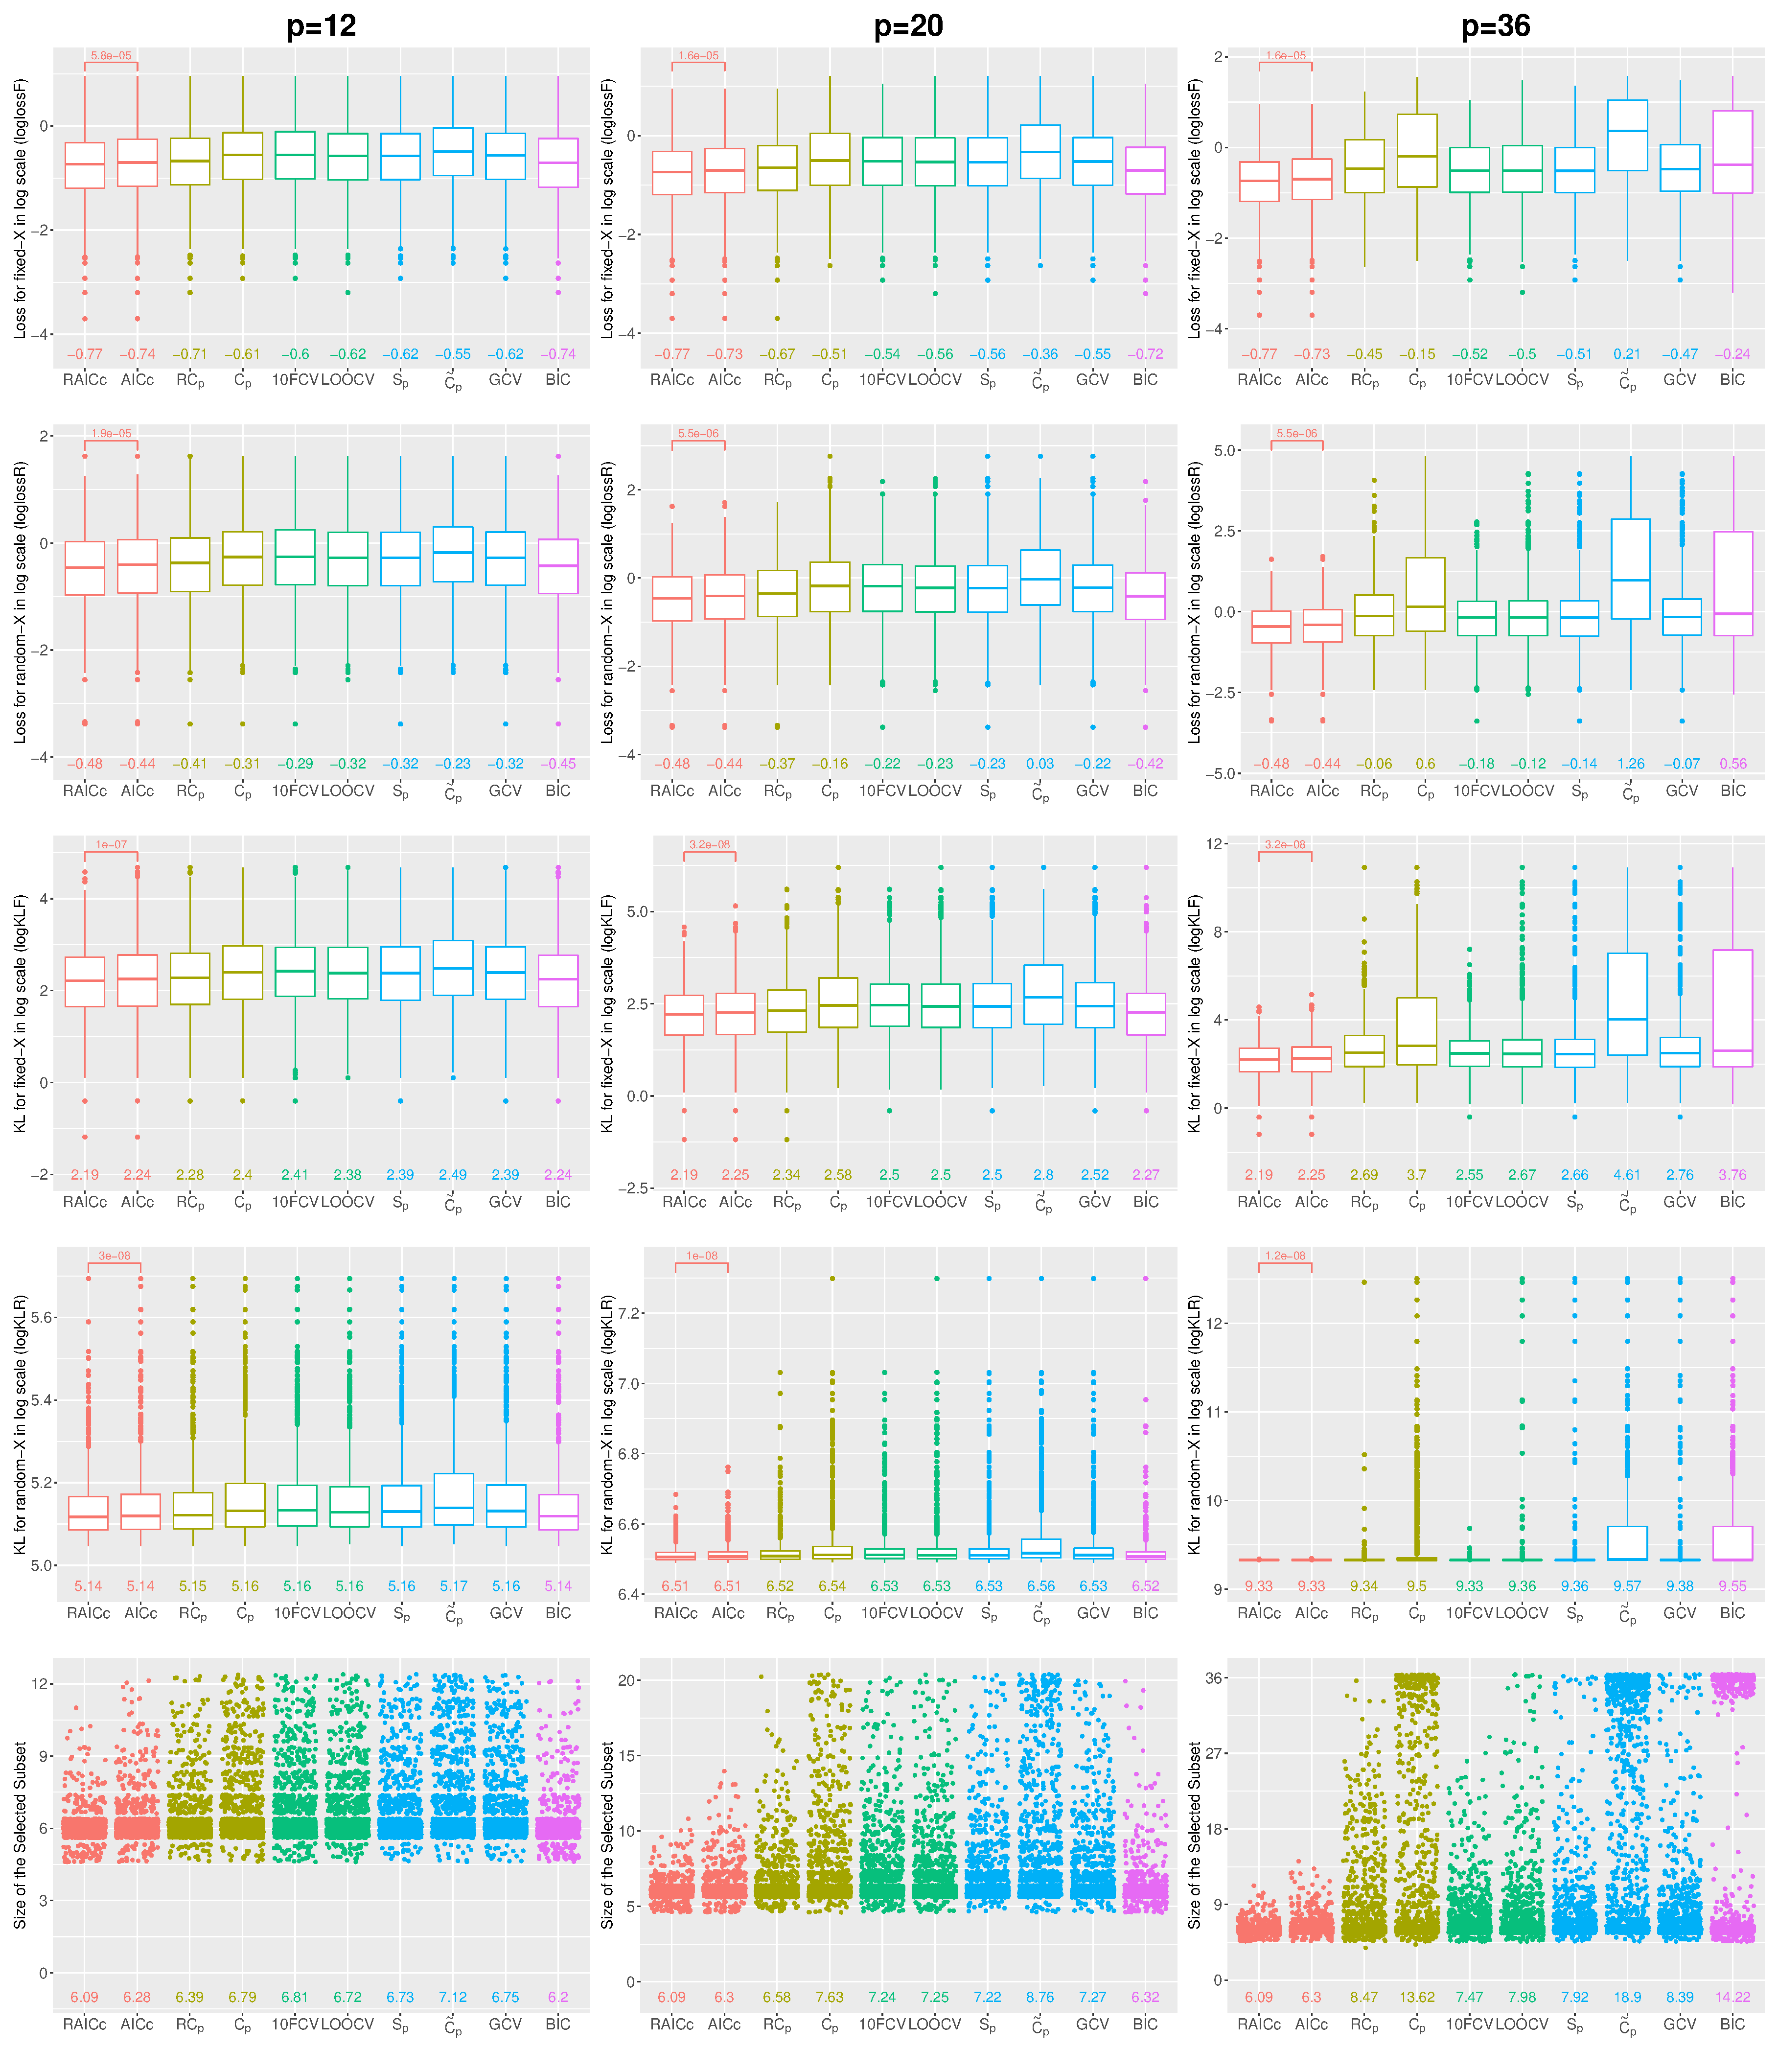
\includegraphics[width=\textwidth]{figures/supplement/fixedx/subset_selection/Sparse-Ex1_n40_hsnr_rho0.eps}
\caption{Variable selection, Fixed-X, Sparse-Ex1, $n=40$, high signal, and $\rho=0$.}
\end{figure}
\clearpage
\begin{figure}[!ht]
\centering
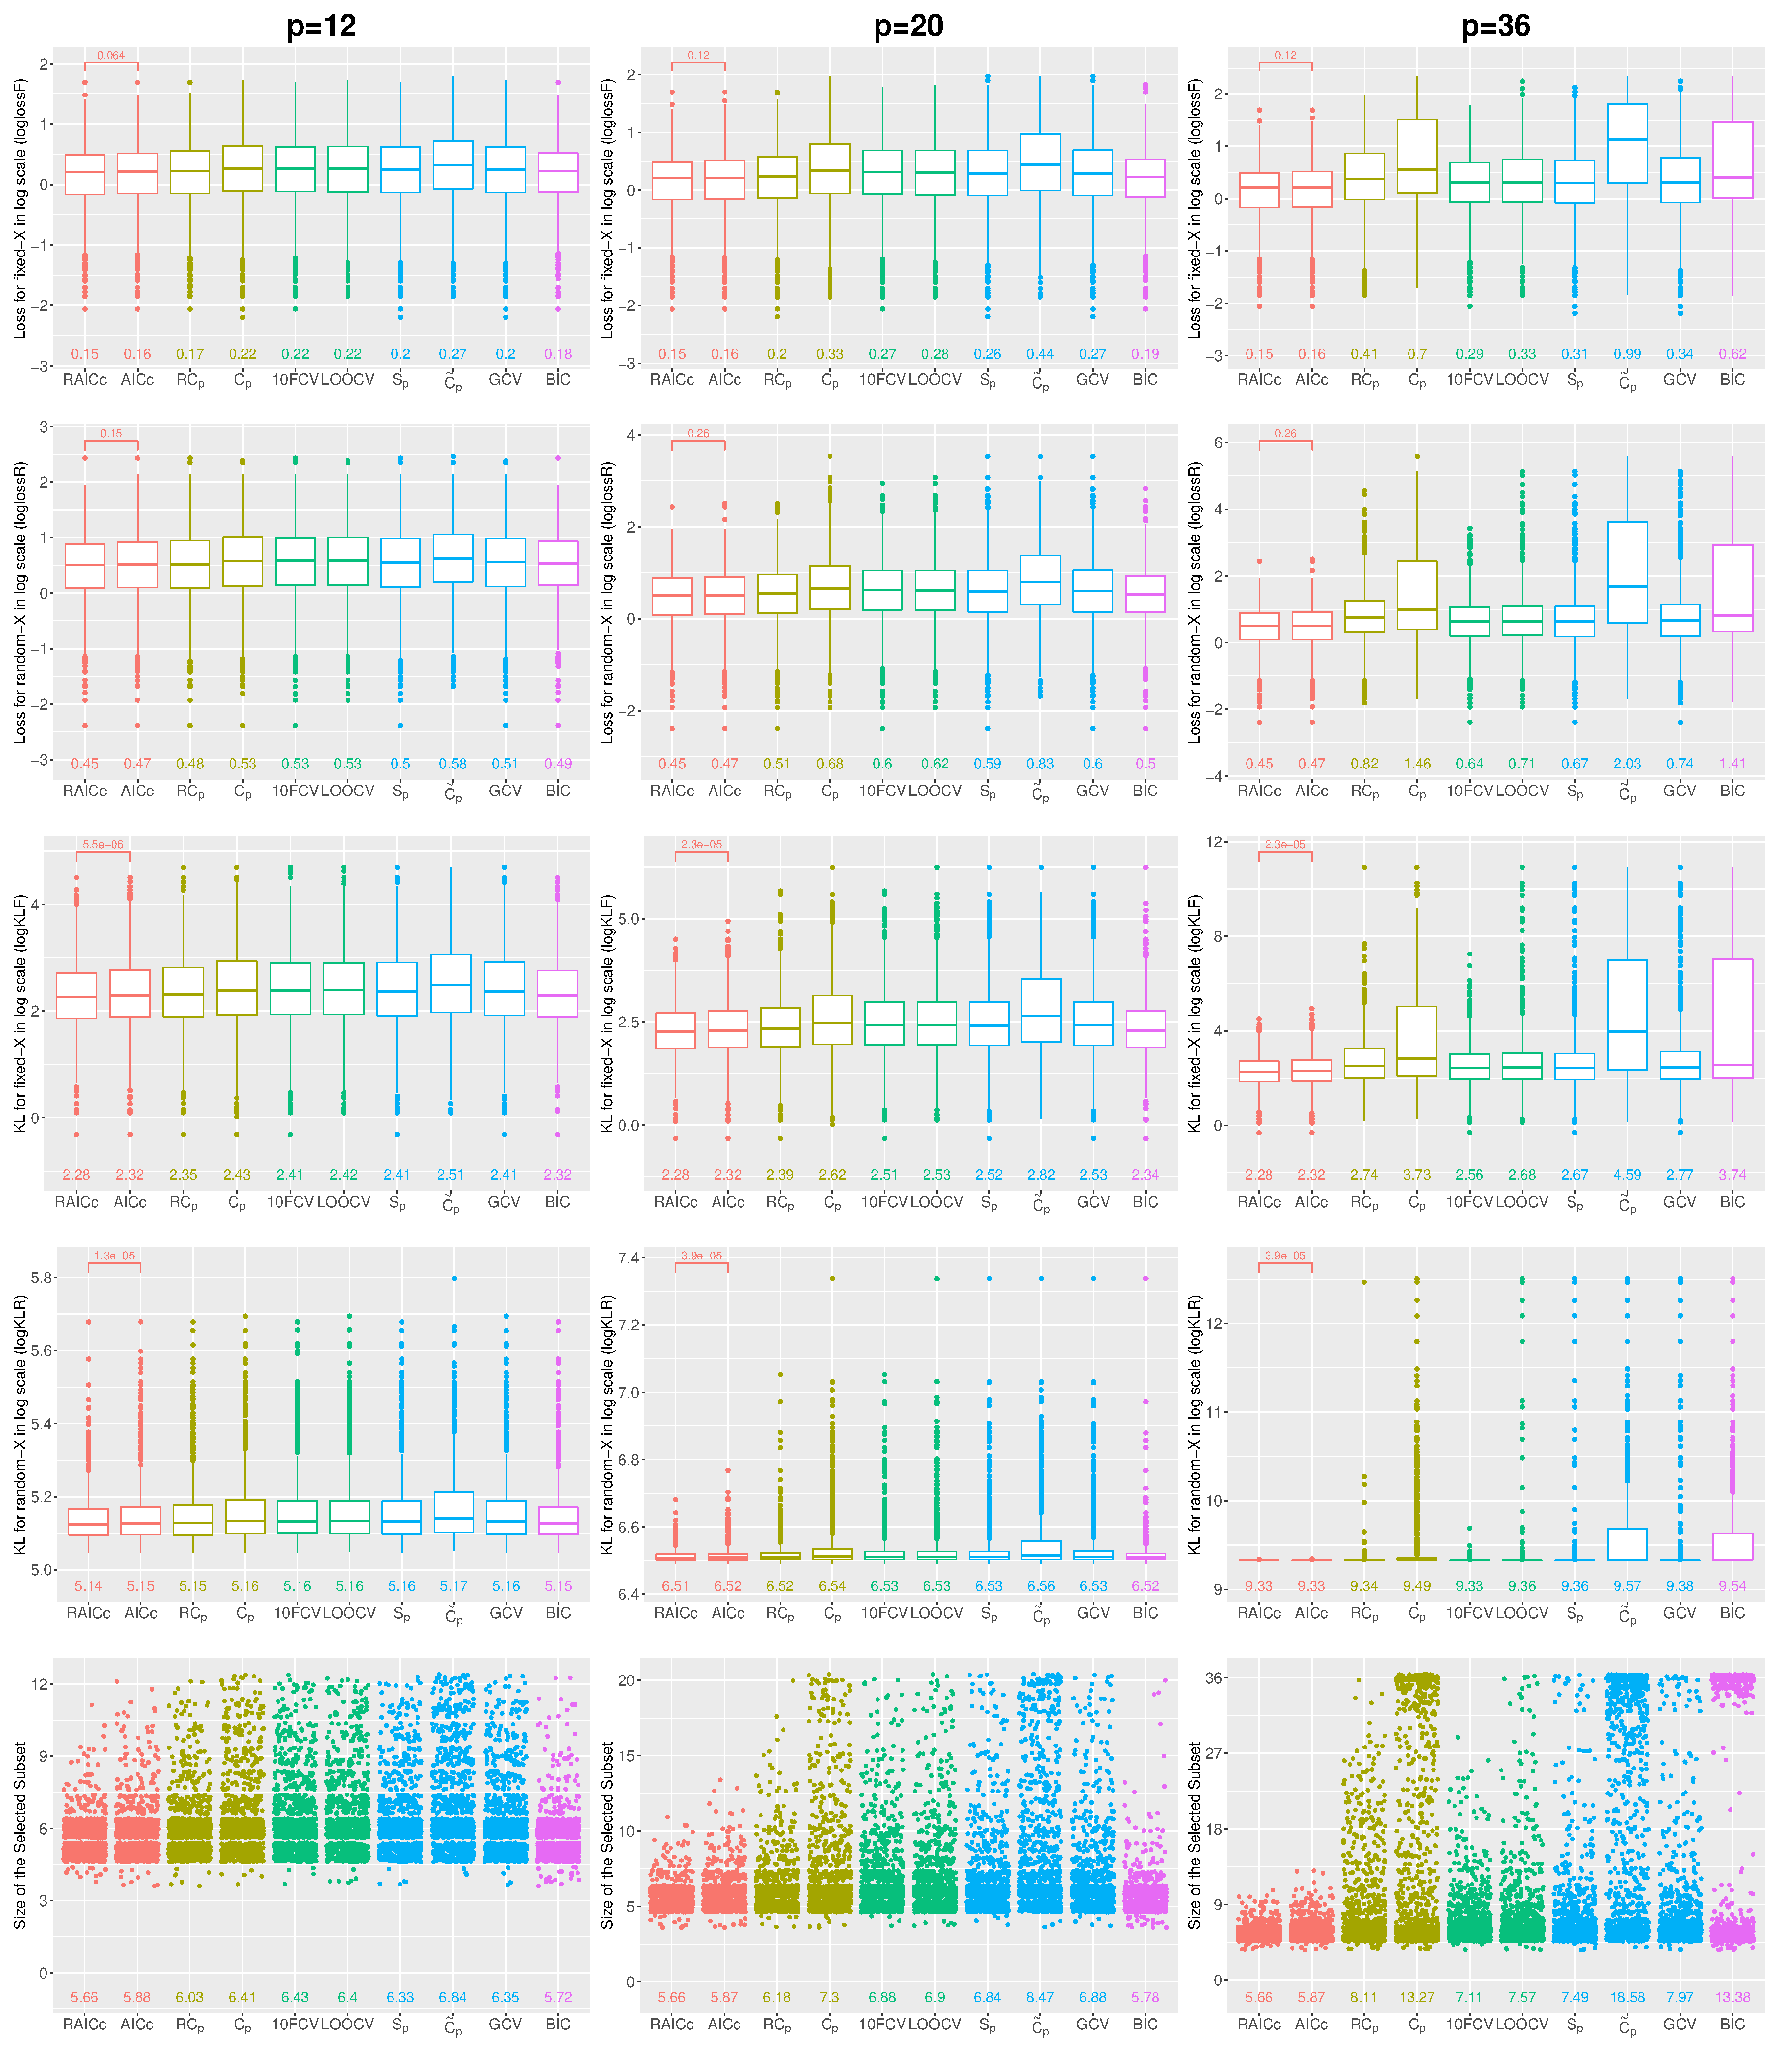
\includegraphics[width=\textwidth]{figures/supplement/fixedx/subset_selection/Sparse-Ex1_n40_hsnr_rho05.eps}
\caption{Variable selection, Fixed-X, Sparse-Ex1, $n=40$, high signal, and $\rho=0.5$.}
\end{figure}
\clearpage
\begin{figure}[!ht]
\centering
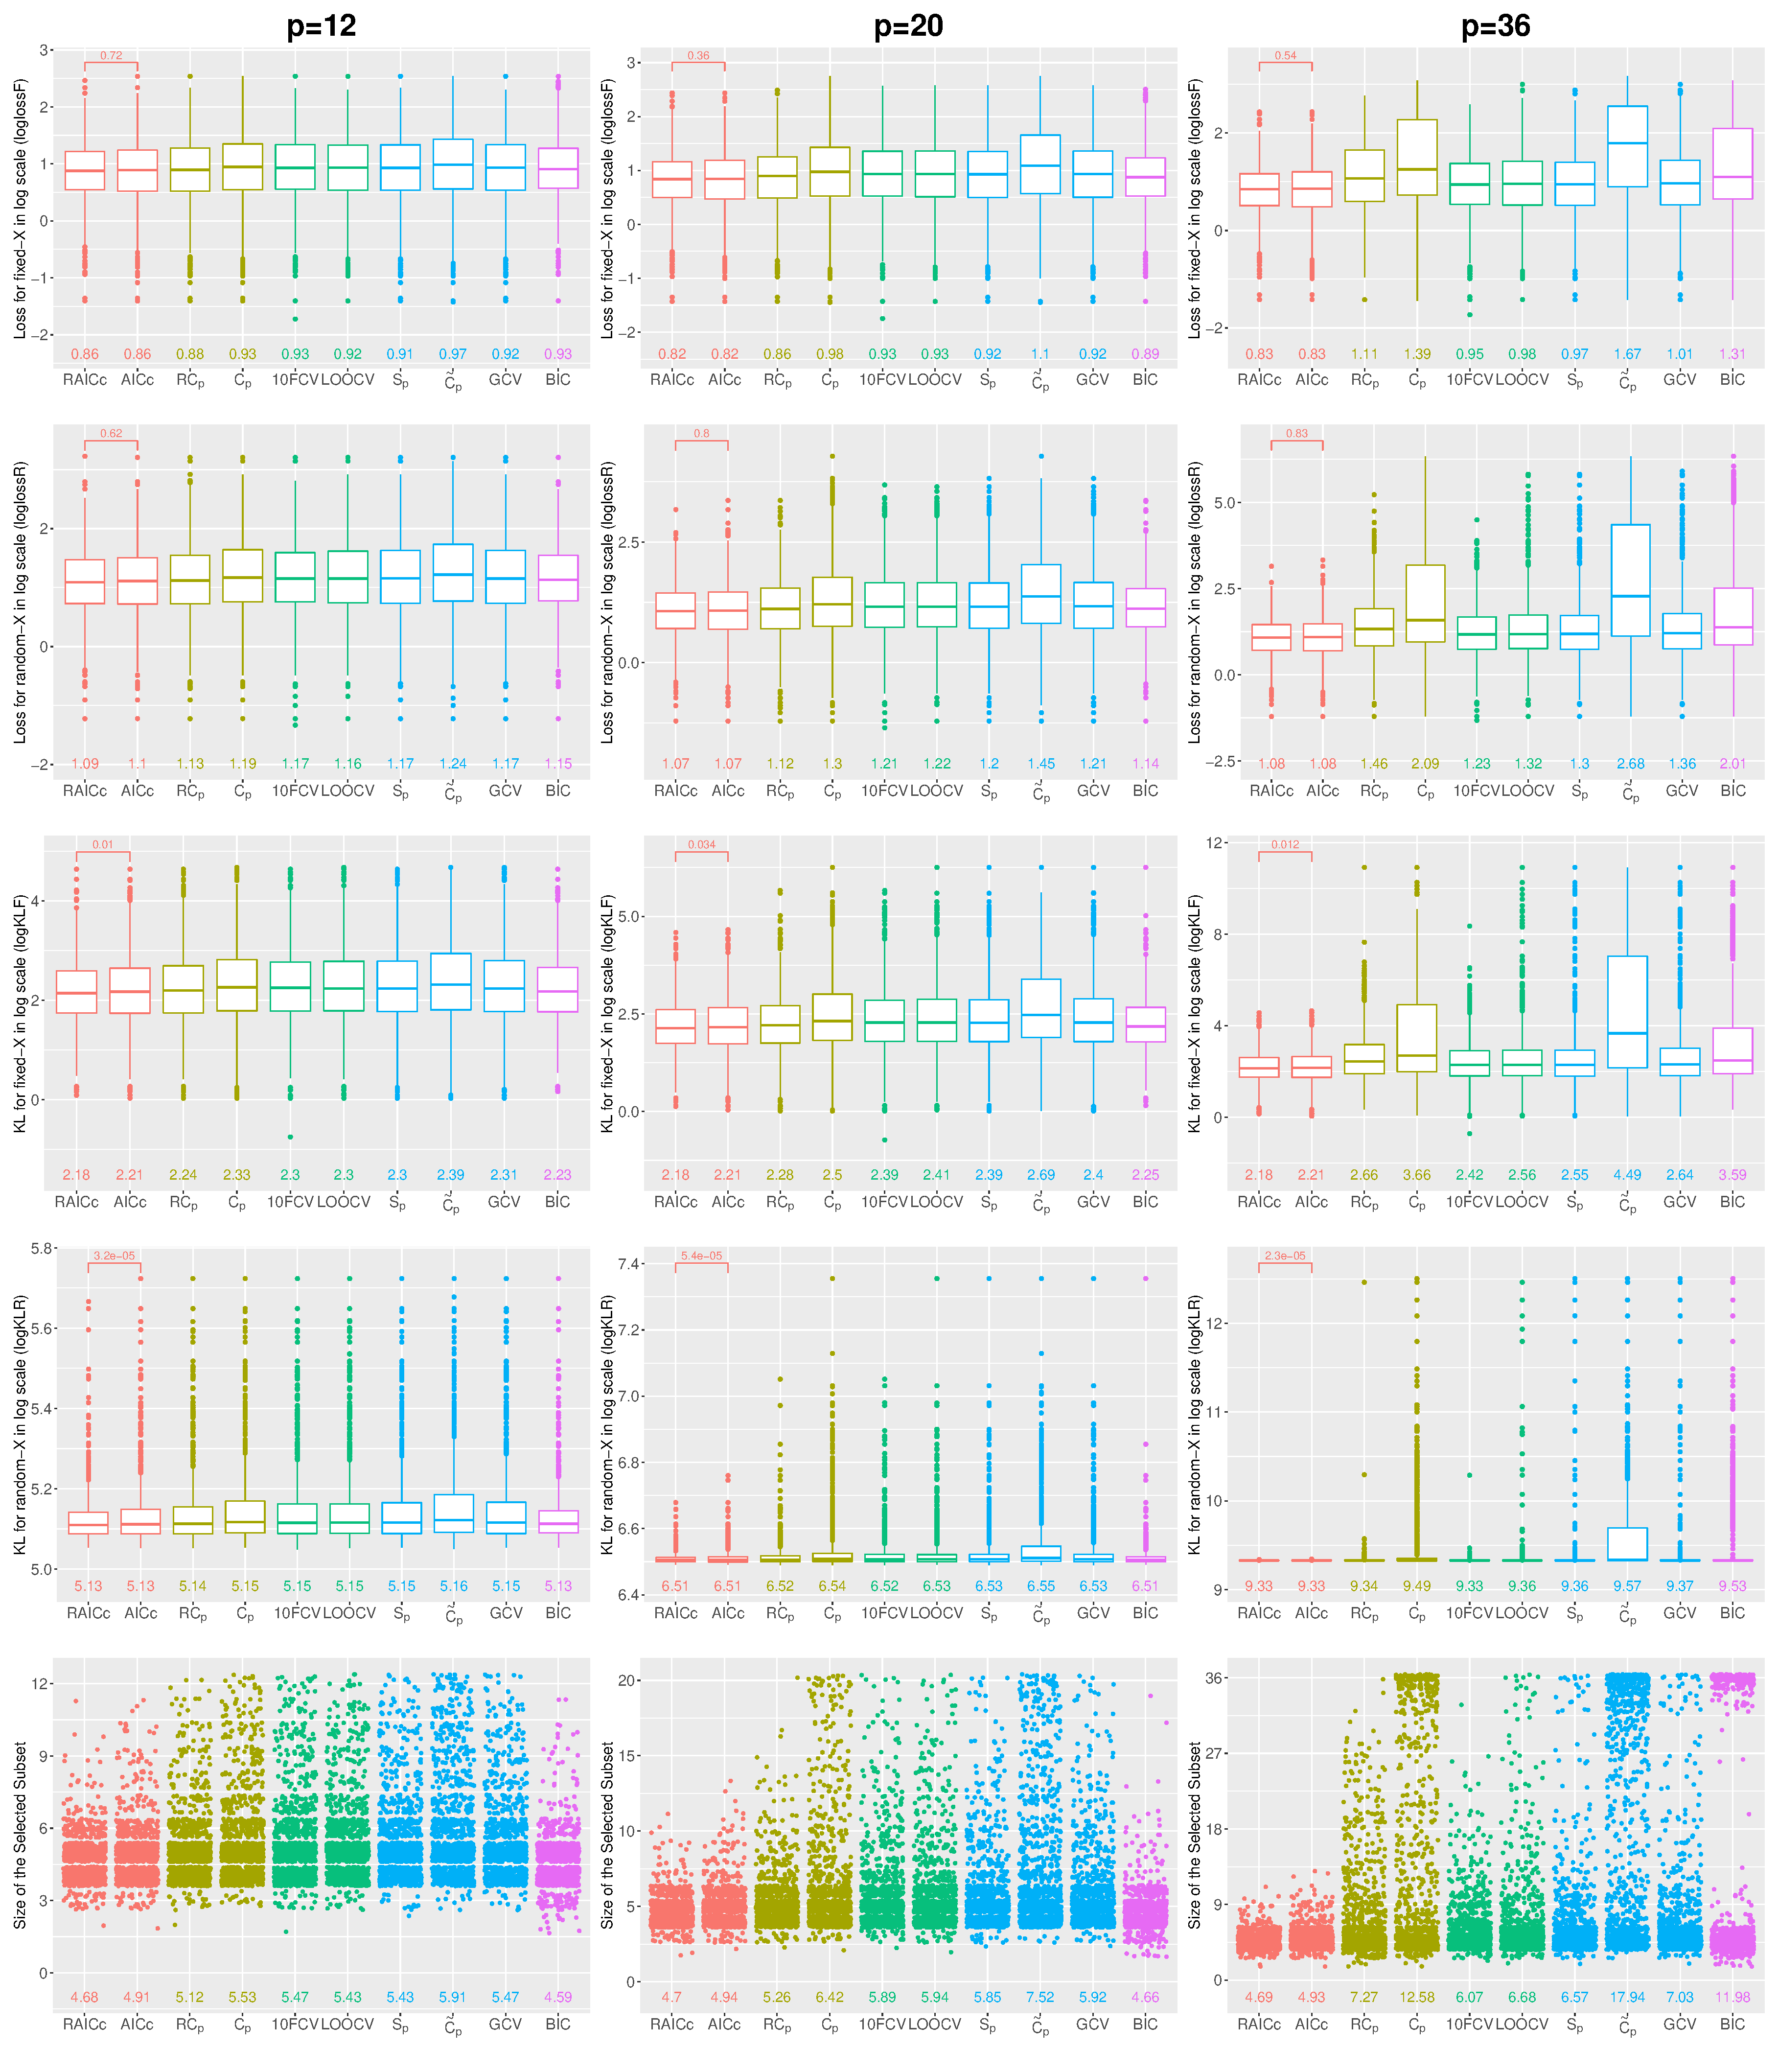
\includegraphics[width=\textwidth]{figures/supplement/fixedx/subset_selection/Sparse-Ex1_n40_hsnr_rho09.eps}
\caption{Variable selection, Fixed-X, Sparse-Ex1, $n=40$, high signal, and $\rho=0.9$.}
\end{figure}
\clearpage
\begin{figure}[!ht]
\centering
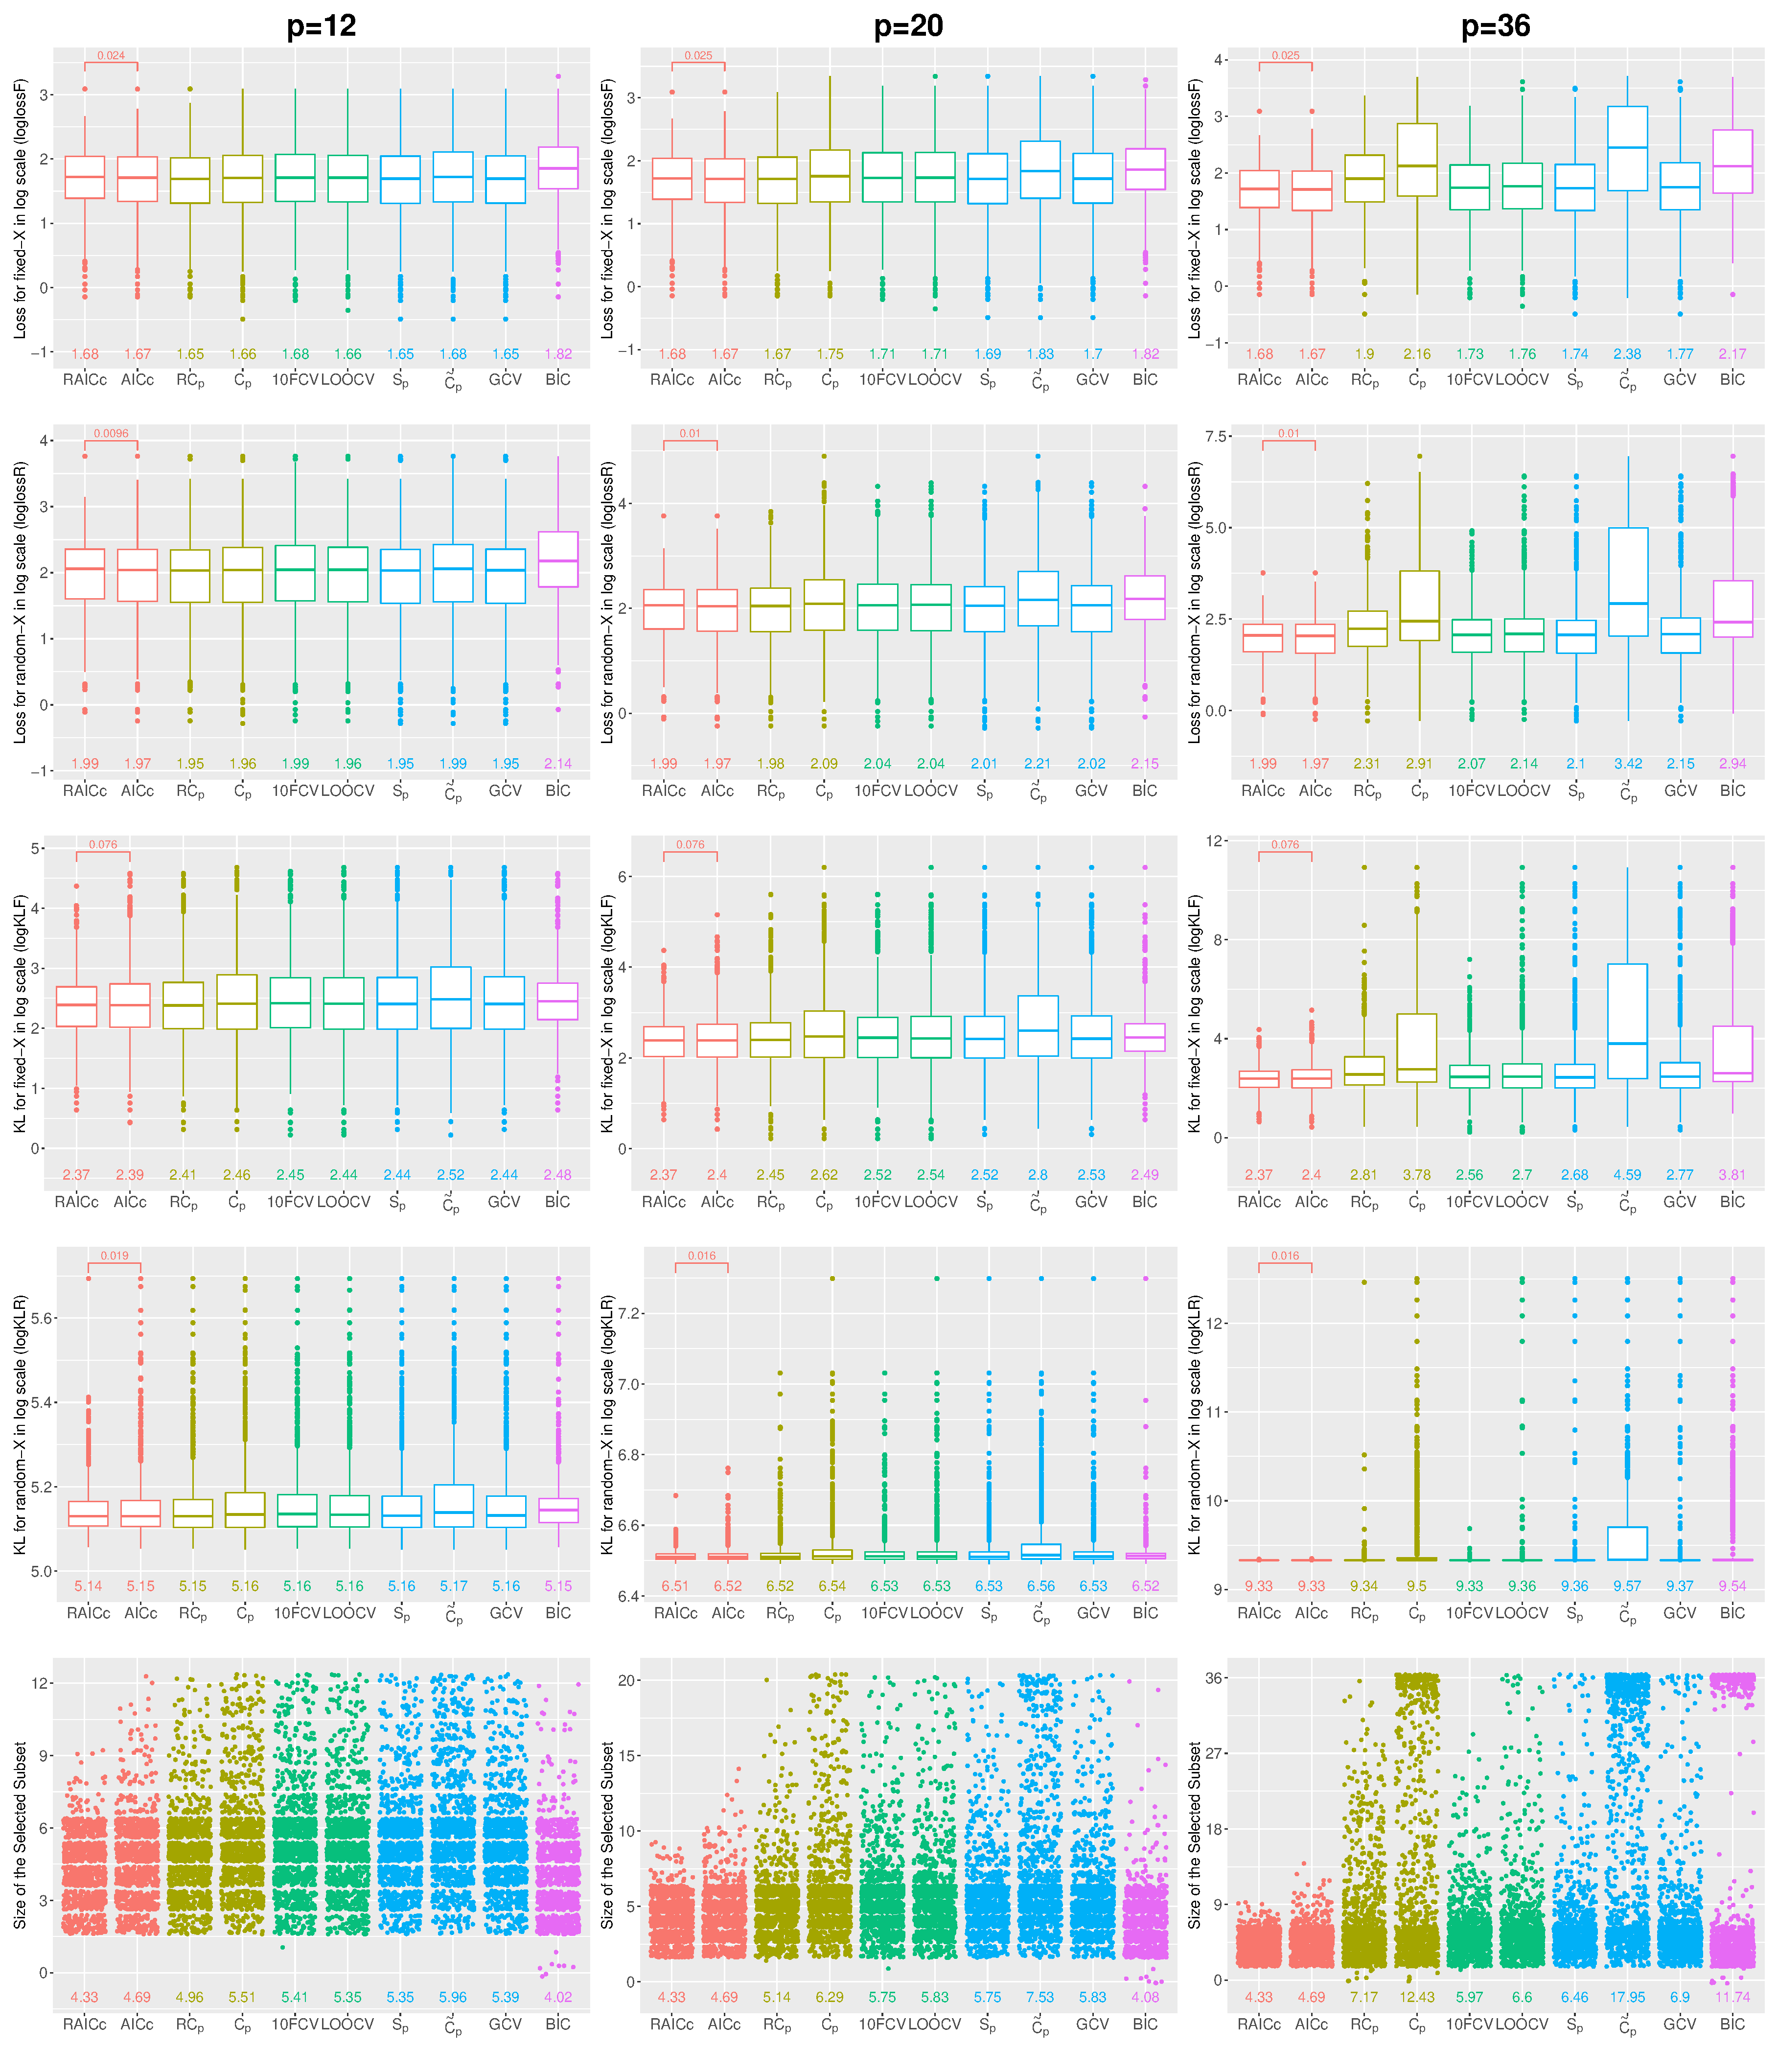
\includegraphics[width=\textwidth]{figures/supplement/fixedx/subset_selection/Sparse-Ex1_n40_msnr_rho0.eps}
\caption{Variable selection, Fixed-X, Sparse-Ex1, $n=40$, medium signal, and $\rho=0$.}
\end{figure}
\clearpage
\begin{figure}[!ht]
\centering
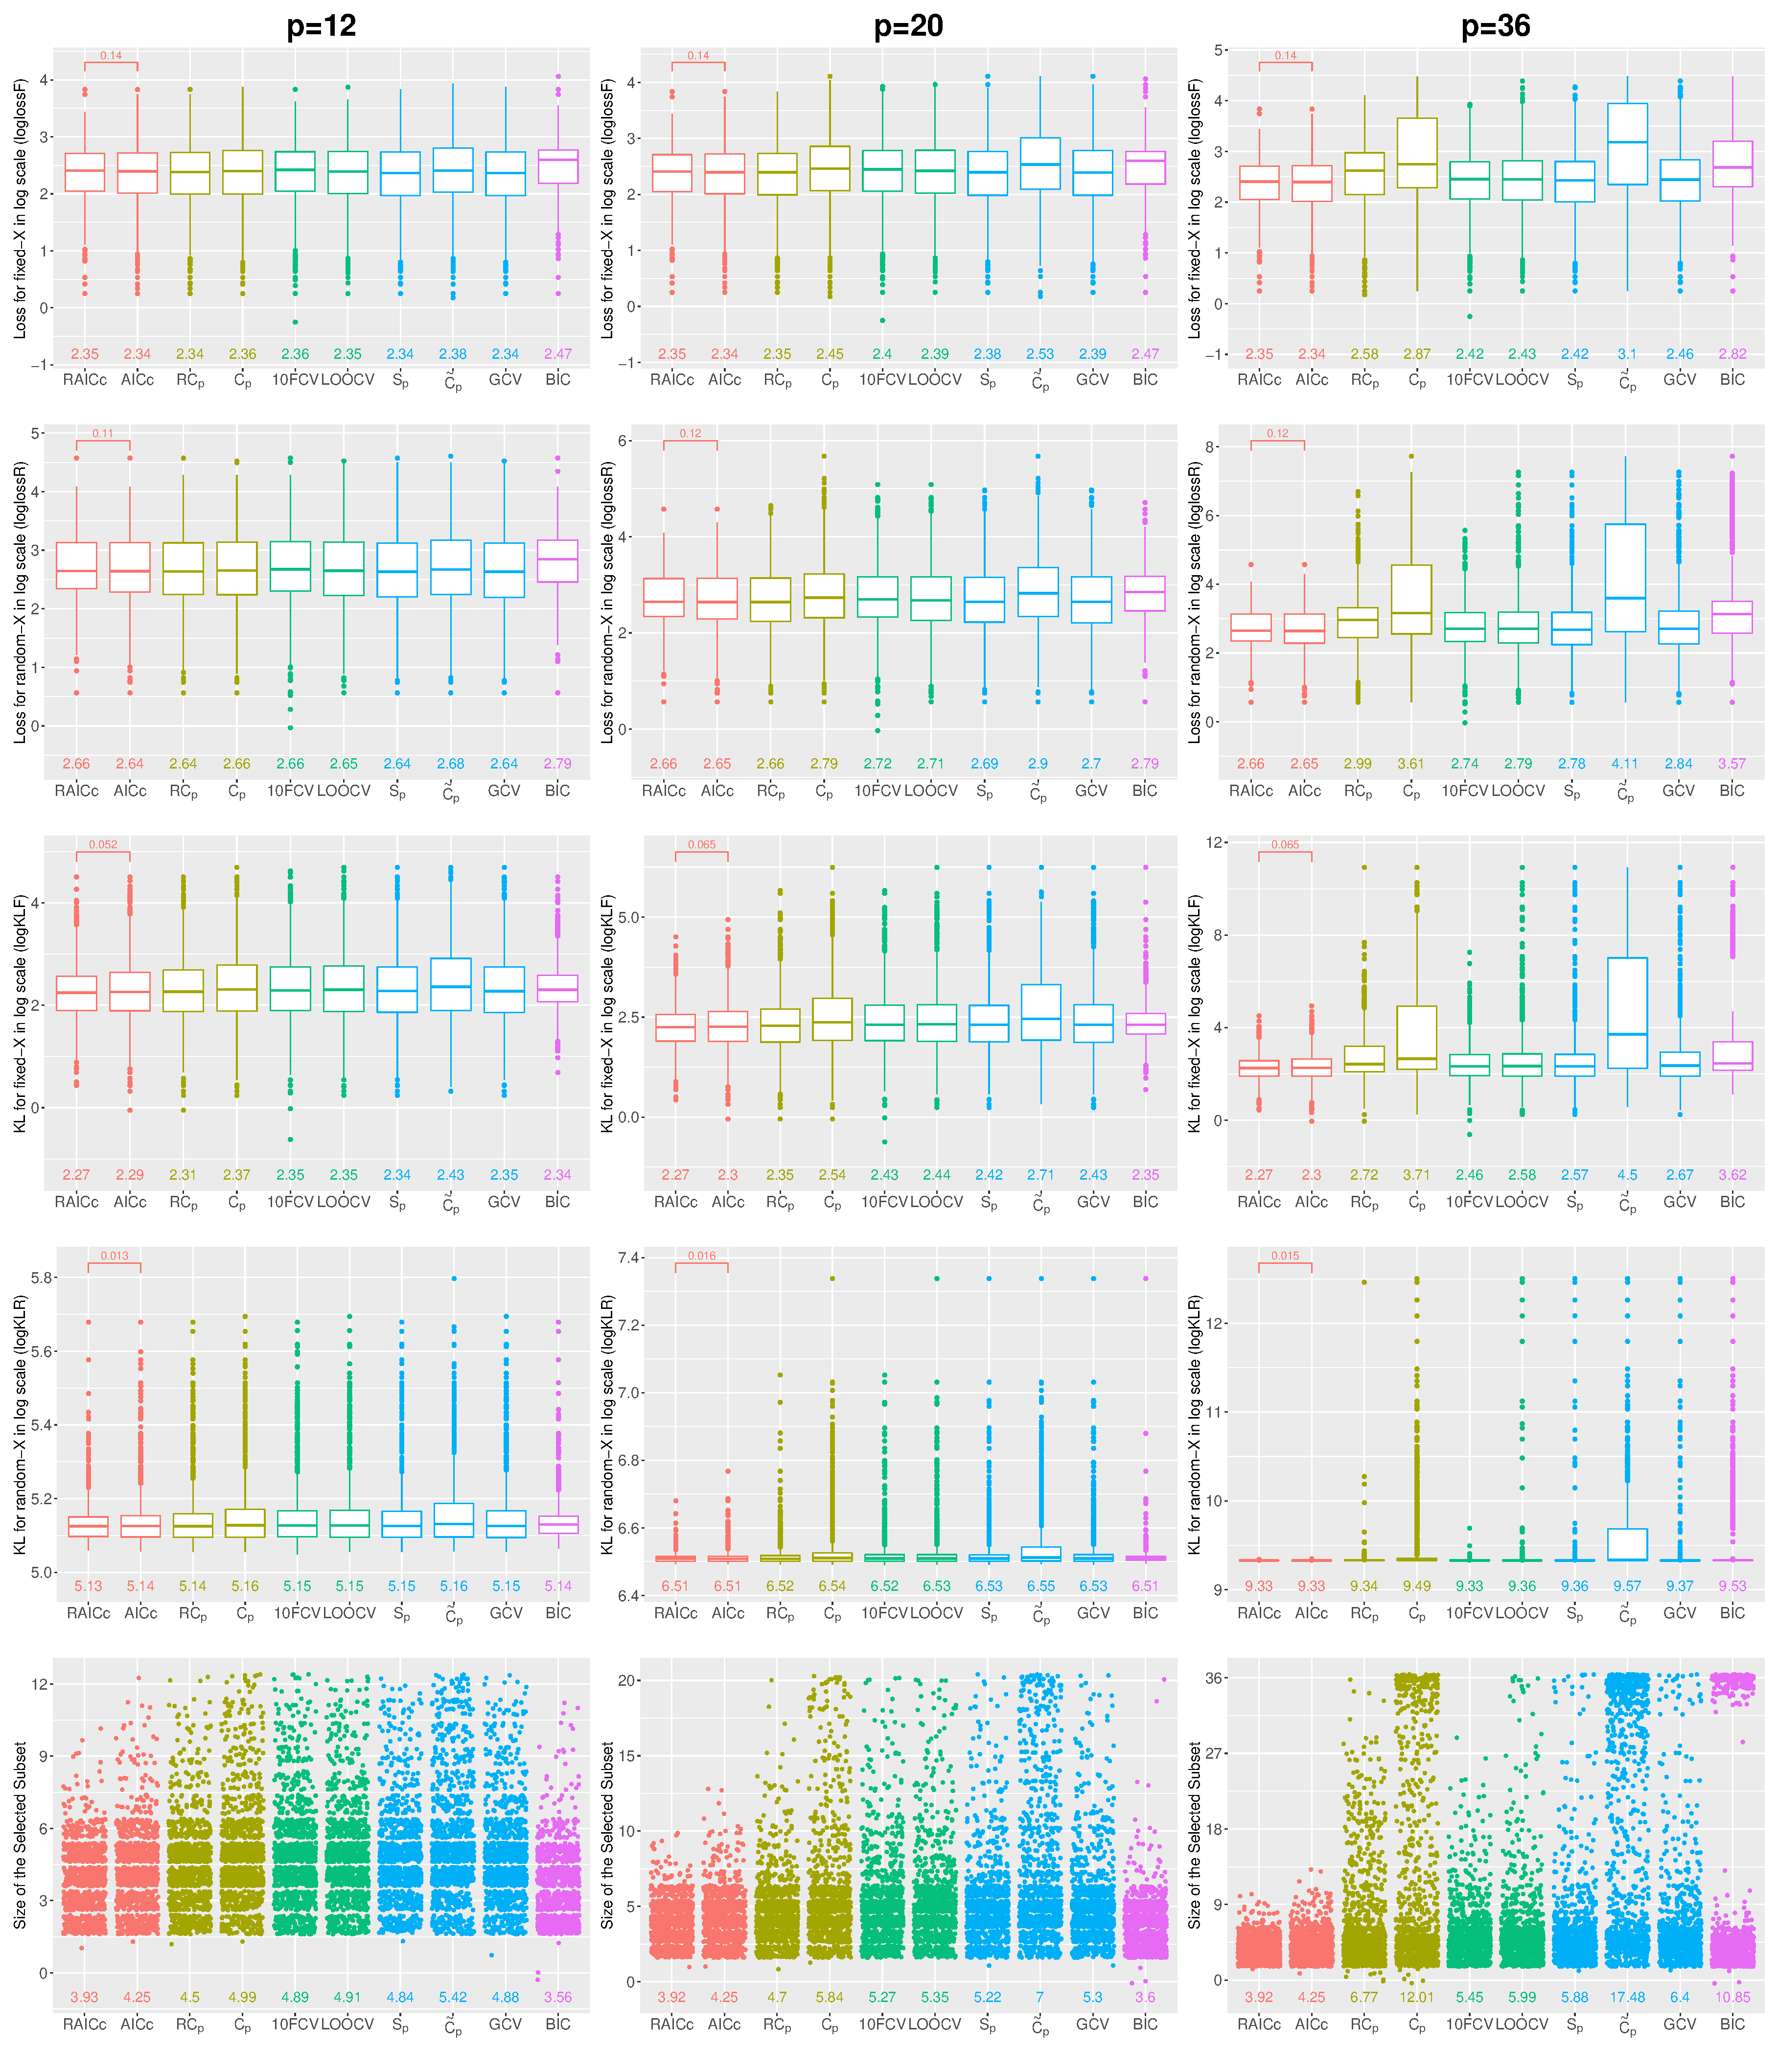
\includegraphics[width=\textwidth]{figures/supplement/fixedx/subset_selection/Sparse-Ex1_n40_msnr_rho05.eps}
\caption{Variable selection, Fixed-X, Sparse-Ex1, $n=40$, medium signal, and $\rho=0.5$.}
\end{figure}
\clearpage
\begin{figure}[!ht]
\centering
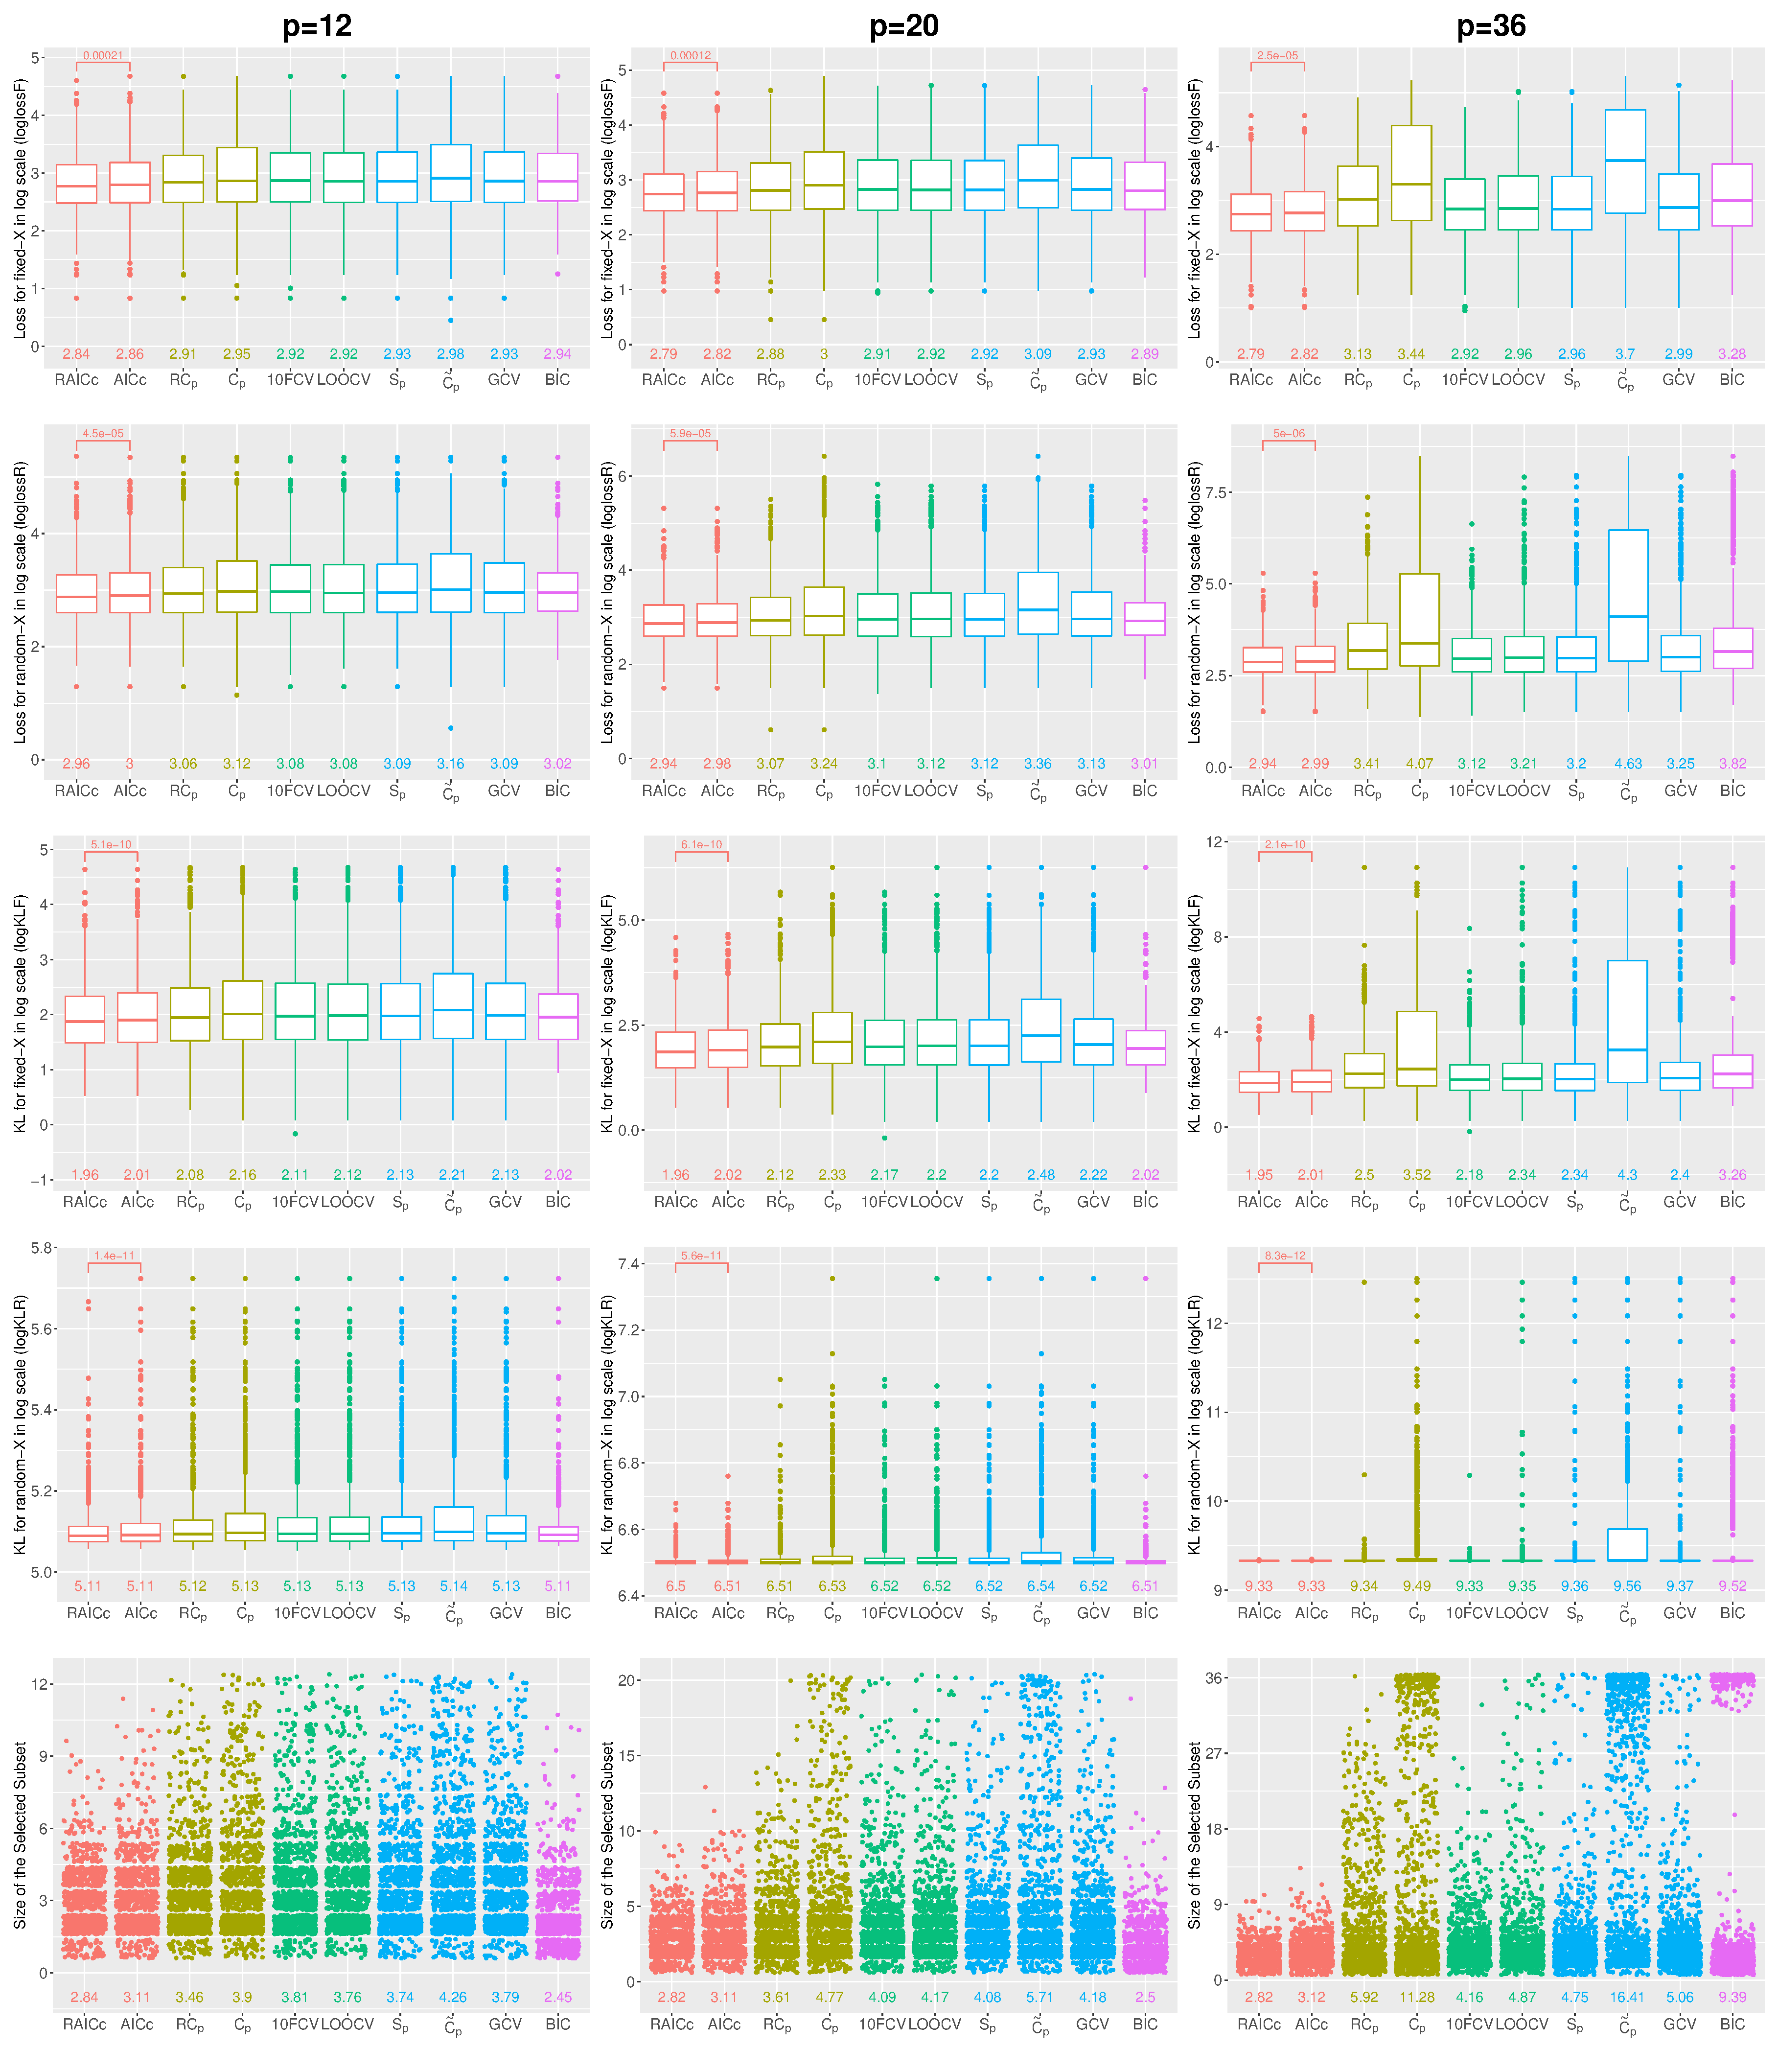
\includegraphics[width=\textwidth]{figures/supplement/fixedx/subset_selection/Sparse-Ex1_n40_msnr_rho09.eps}
\caption{Variable selection, Fixed-X, Sparse-Ex1, $n=40$, medium signal, and $\rho=0.9$.}
\end{figure}
\clearpage
\begin{figure}[!ht]
\centering
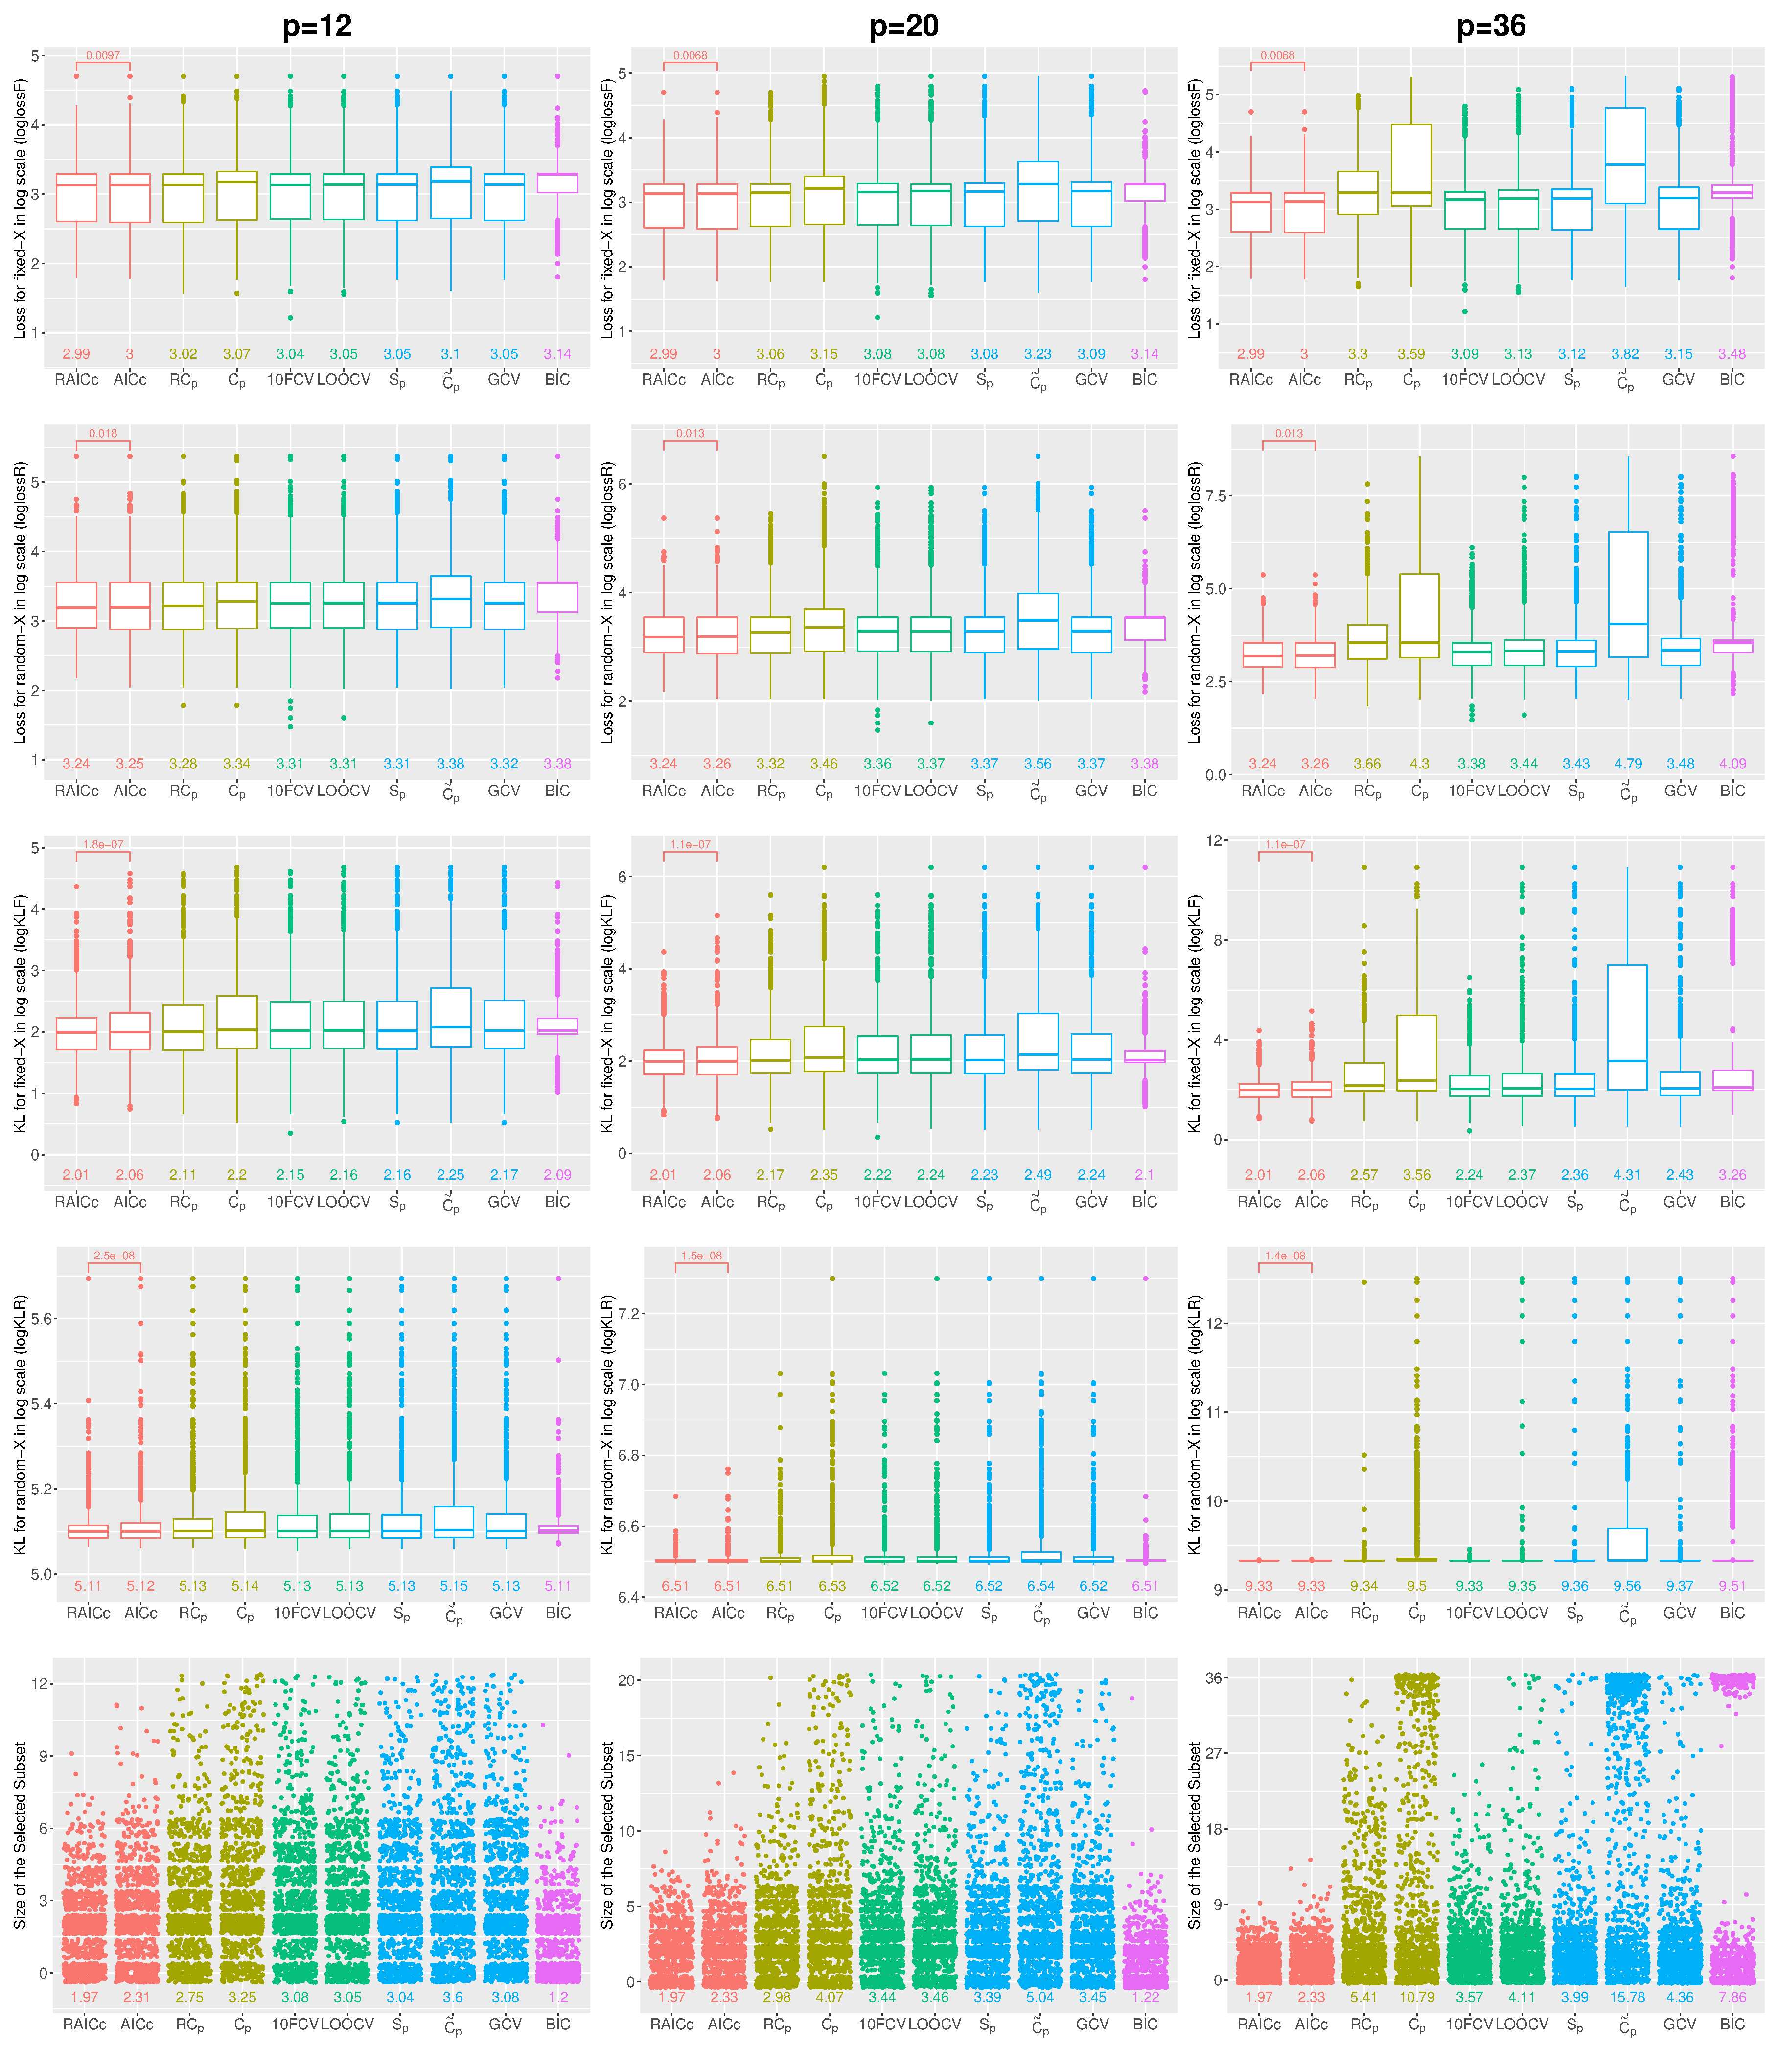
\includegraphics[width=\textwidth]{figures/supplement/fixedx/subset_selection/Sparse-Ex1_n40_lsnr_rho0.eps}
\caption{Variable selection, Fixed-X, Sparse-Ex1, $n=40$, low signal, and $\rho=0$.}
\end{figure}
\clearpage
\begin{figure}[!ht]
\centering
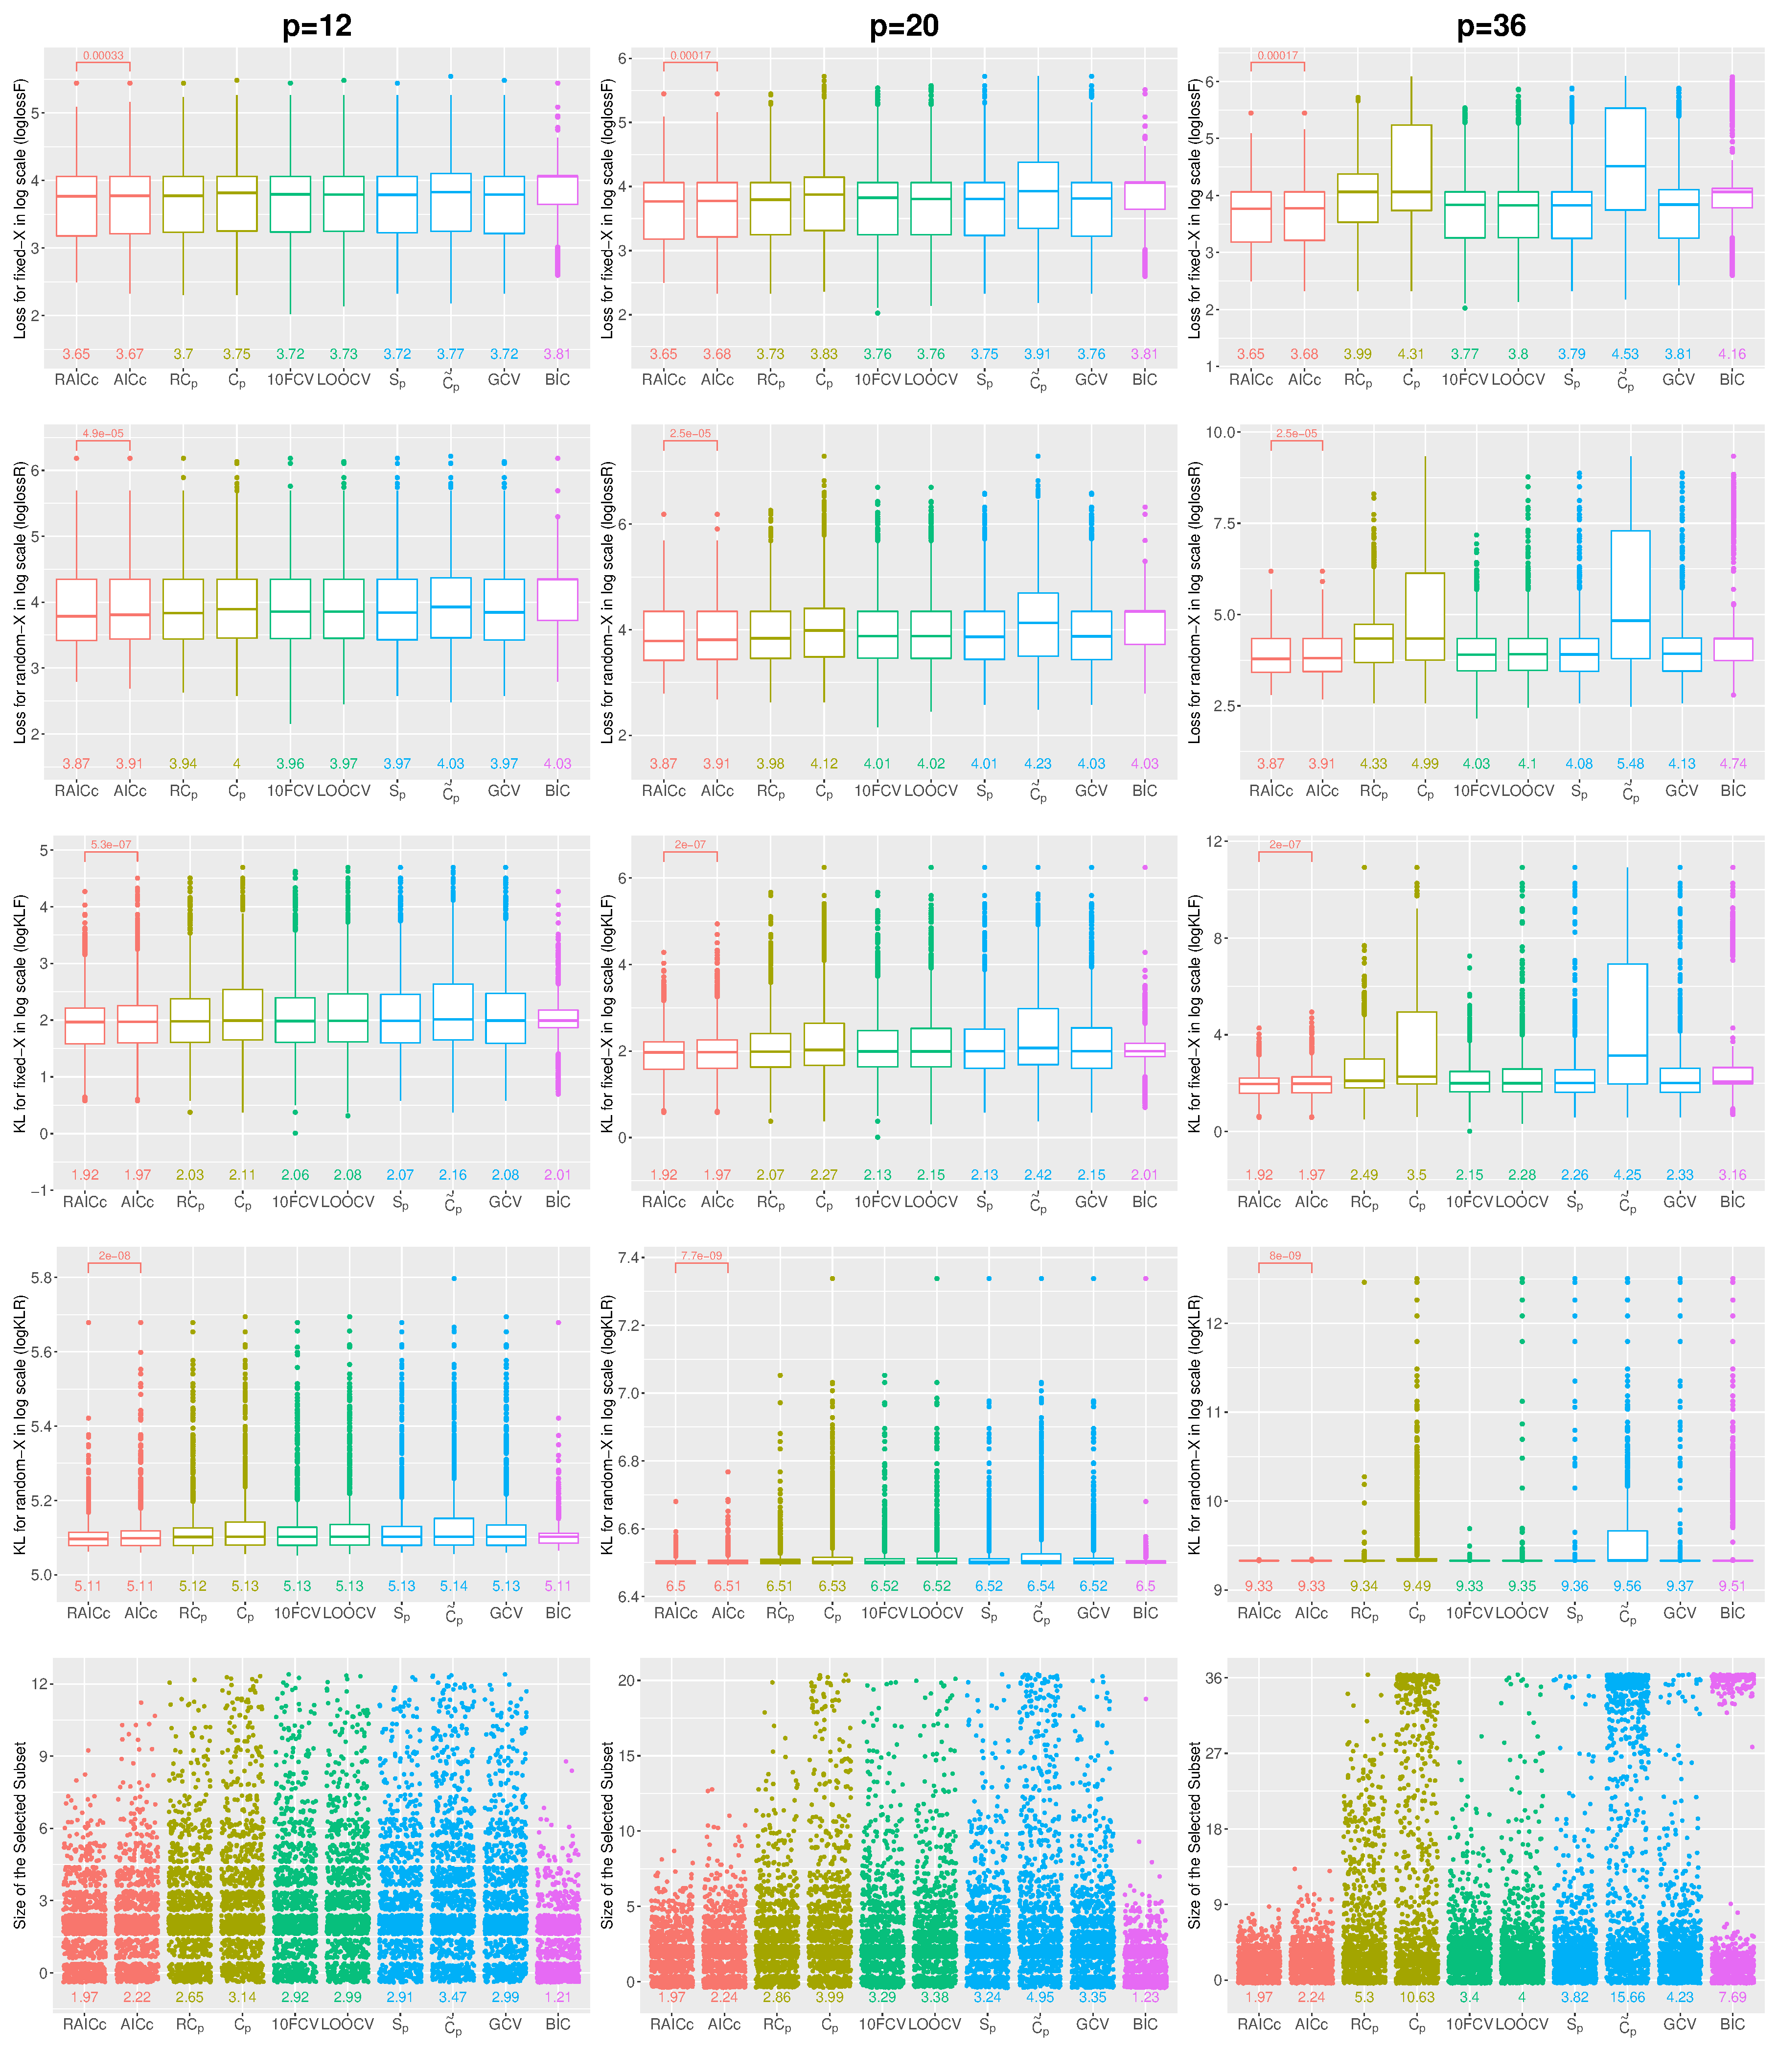
\includegraphics[width=\textwidth]{figures/supplement/fixedx/subset_selection/Sparse-Ex1_n40_lsnr_rho05.eps}
\caption{Variable selection, Fixed-X, Sparse-Ex1, $n=40$, low signal, and $\rho=0.5$.}
\end{figure}
\clearpage
\begin{figure}[!ht]
\centering
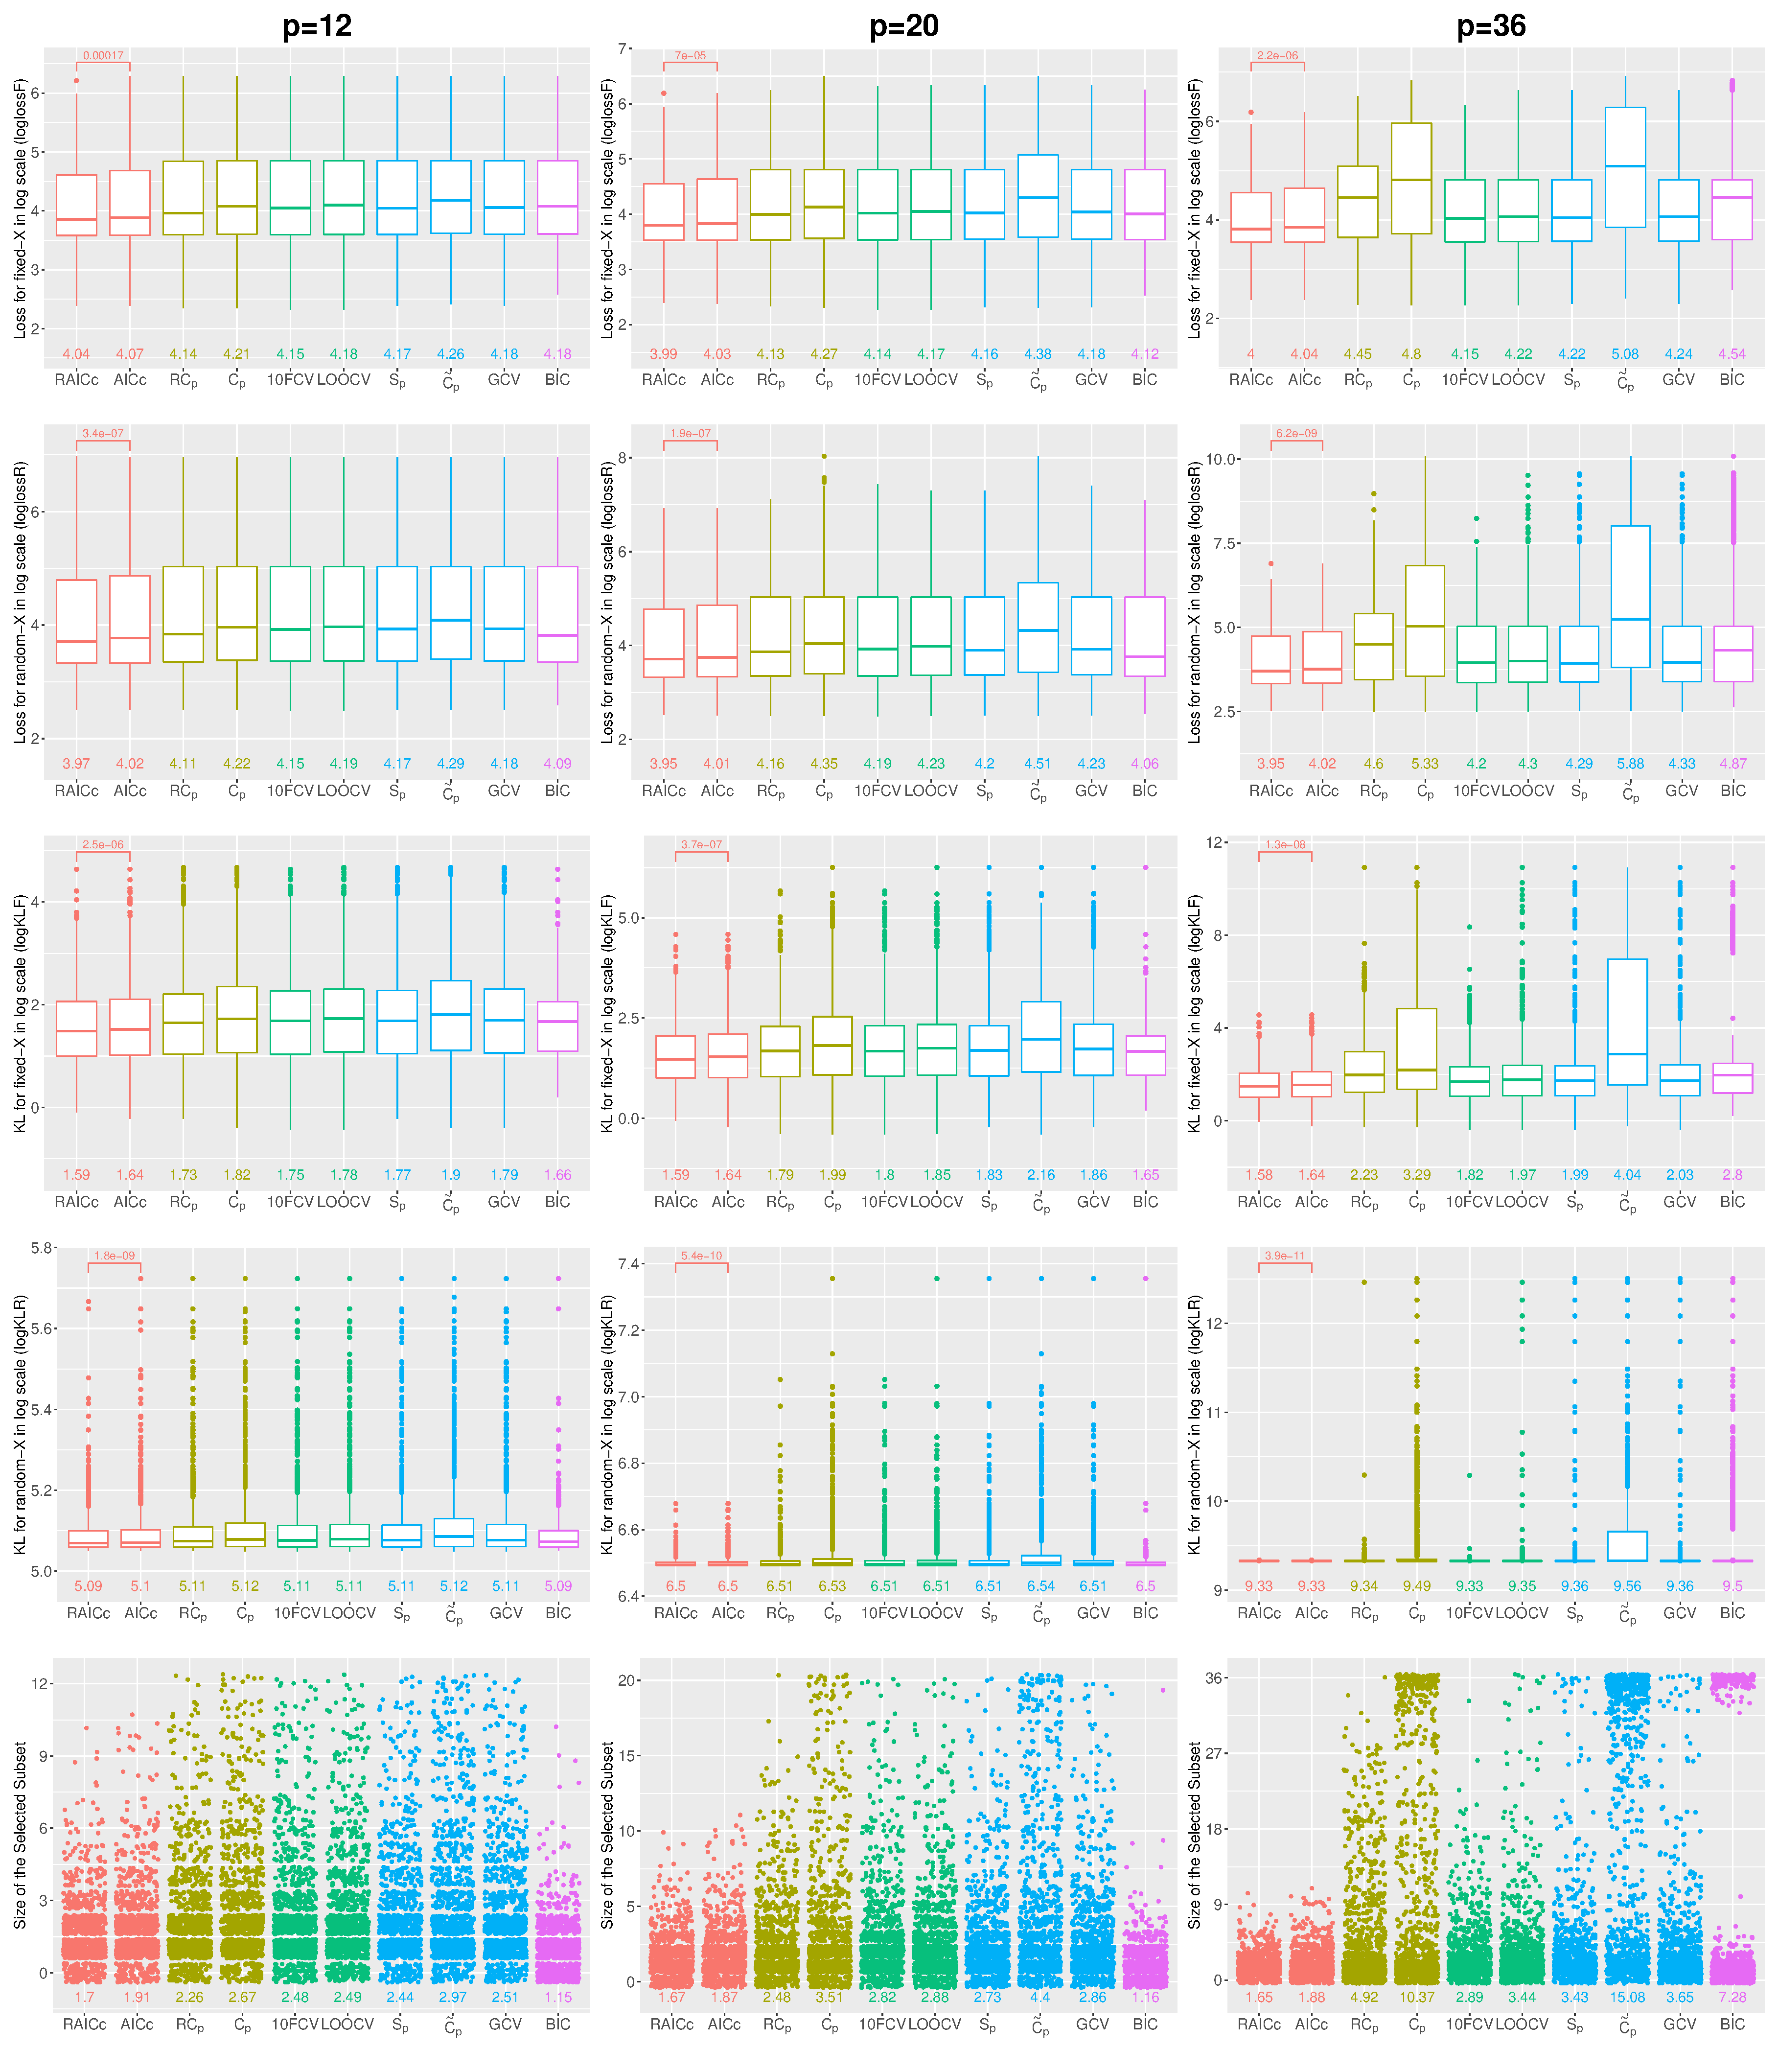
\includegraphics[width=\textwidth]{figures/supplement/fixedx/subset_selection/Sparse-Ex1_n40_lsnr_rho09.eps}
\caption{Variable selection, Fixed-X, Sparse-Ex1, $n=40$, low signal, and $\rho=0.9$.}
\end{figure}
\clearpage
\begin{figure}[!ht]
\centering
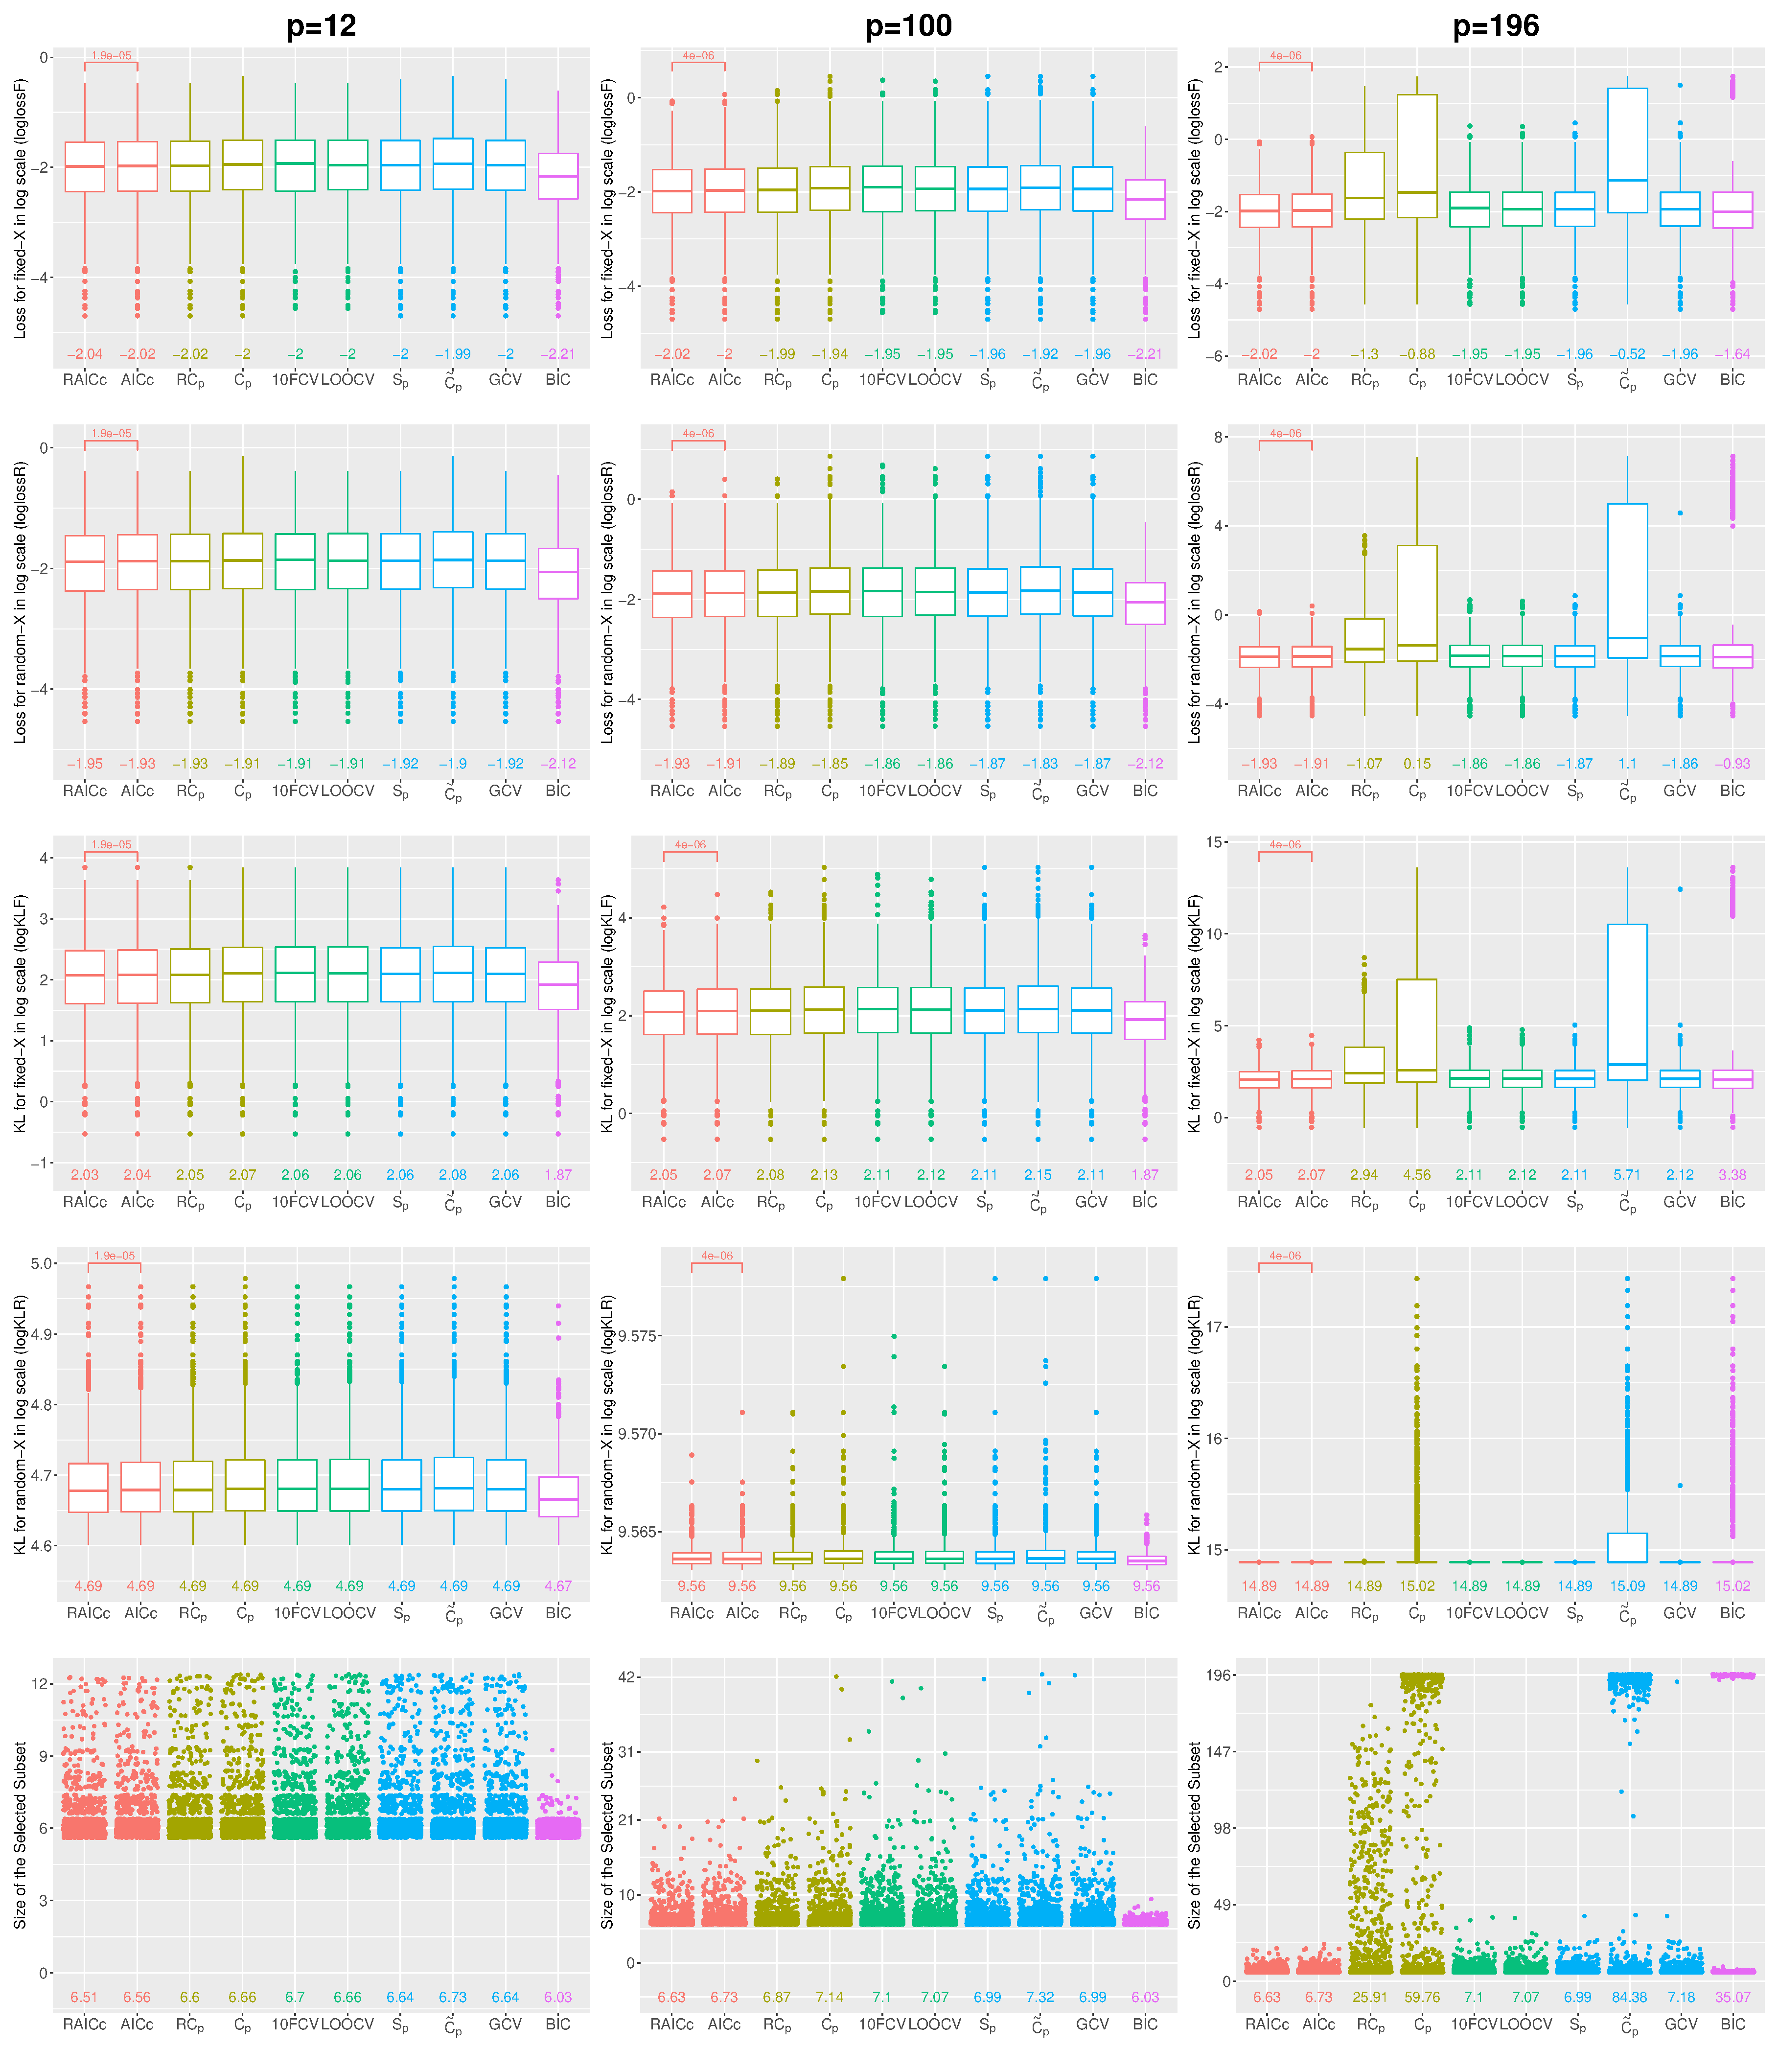
\includegraphics[width=\textwidth]{figures/supplement/fixedx/subset_selection/Sparse-Ex1_n200_hsnr_rho0.eps}
\caption{Variable selection, Fixed-X, Sparse-Ex1, $n=200$, high signal, and $\rho=0$.}
\end{figure}
\clearpage
\begin{figure}[!ht]
\centering
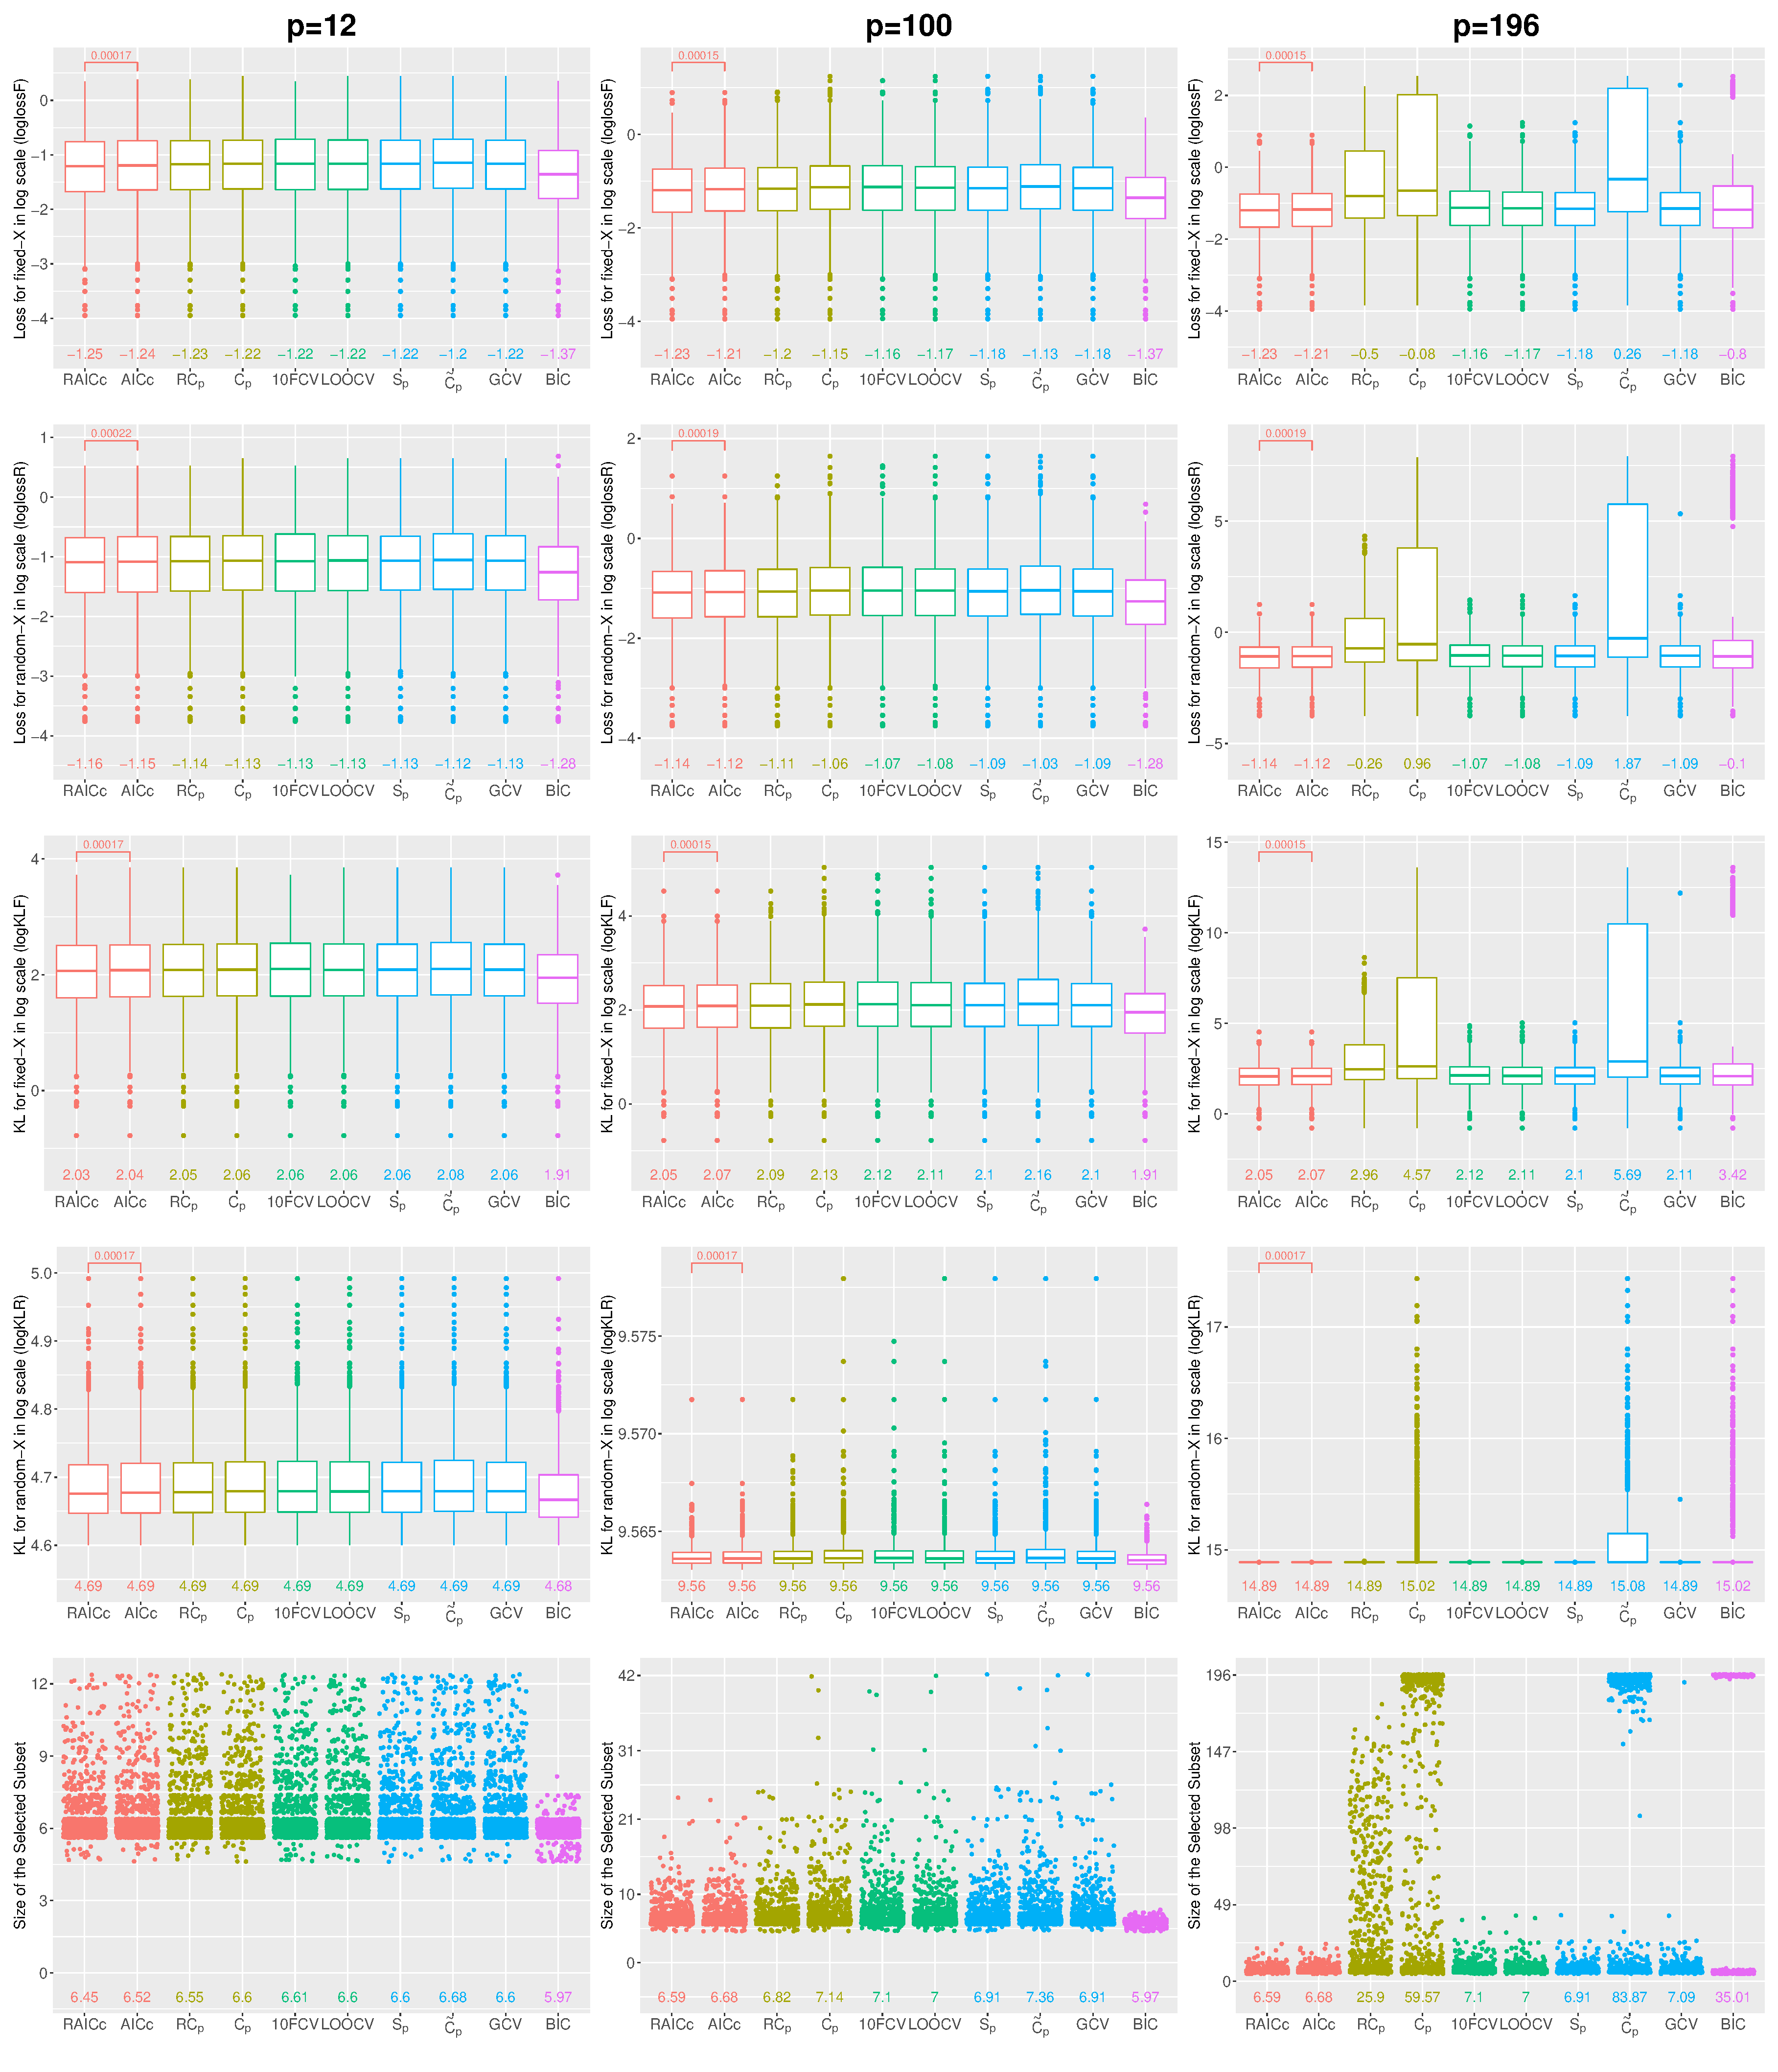
\includegraphics[width=\textwidth]{figures/supplement/fixedx/subset_selection/Sparse-Ex1_n200_hsnr_rho05.eps}
\caption{Variable selection, Fixed-X, Sparse-Ex1, $n=200$, high signal, and $\rho=0.5$.}
\end{figure}
\clearpage
\begin{figure}[!ht]
\centering
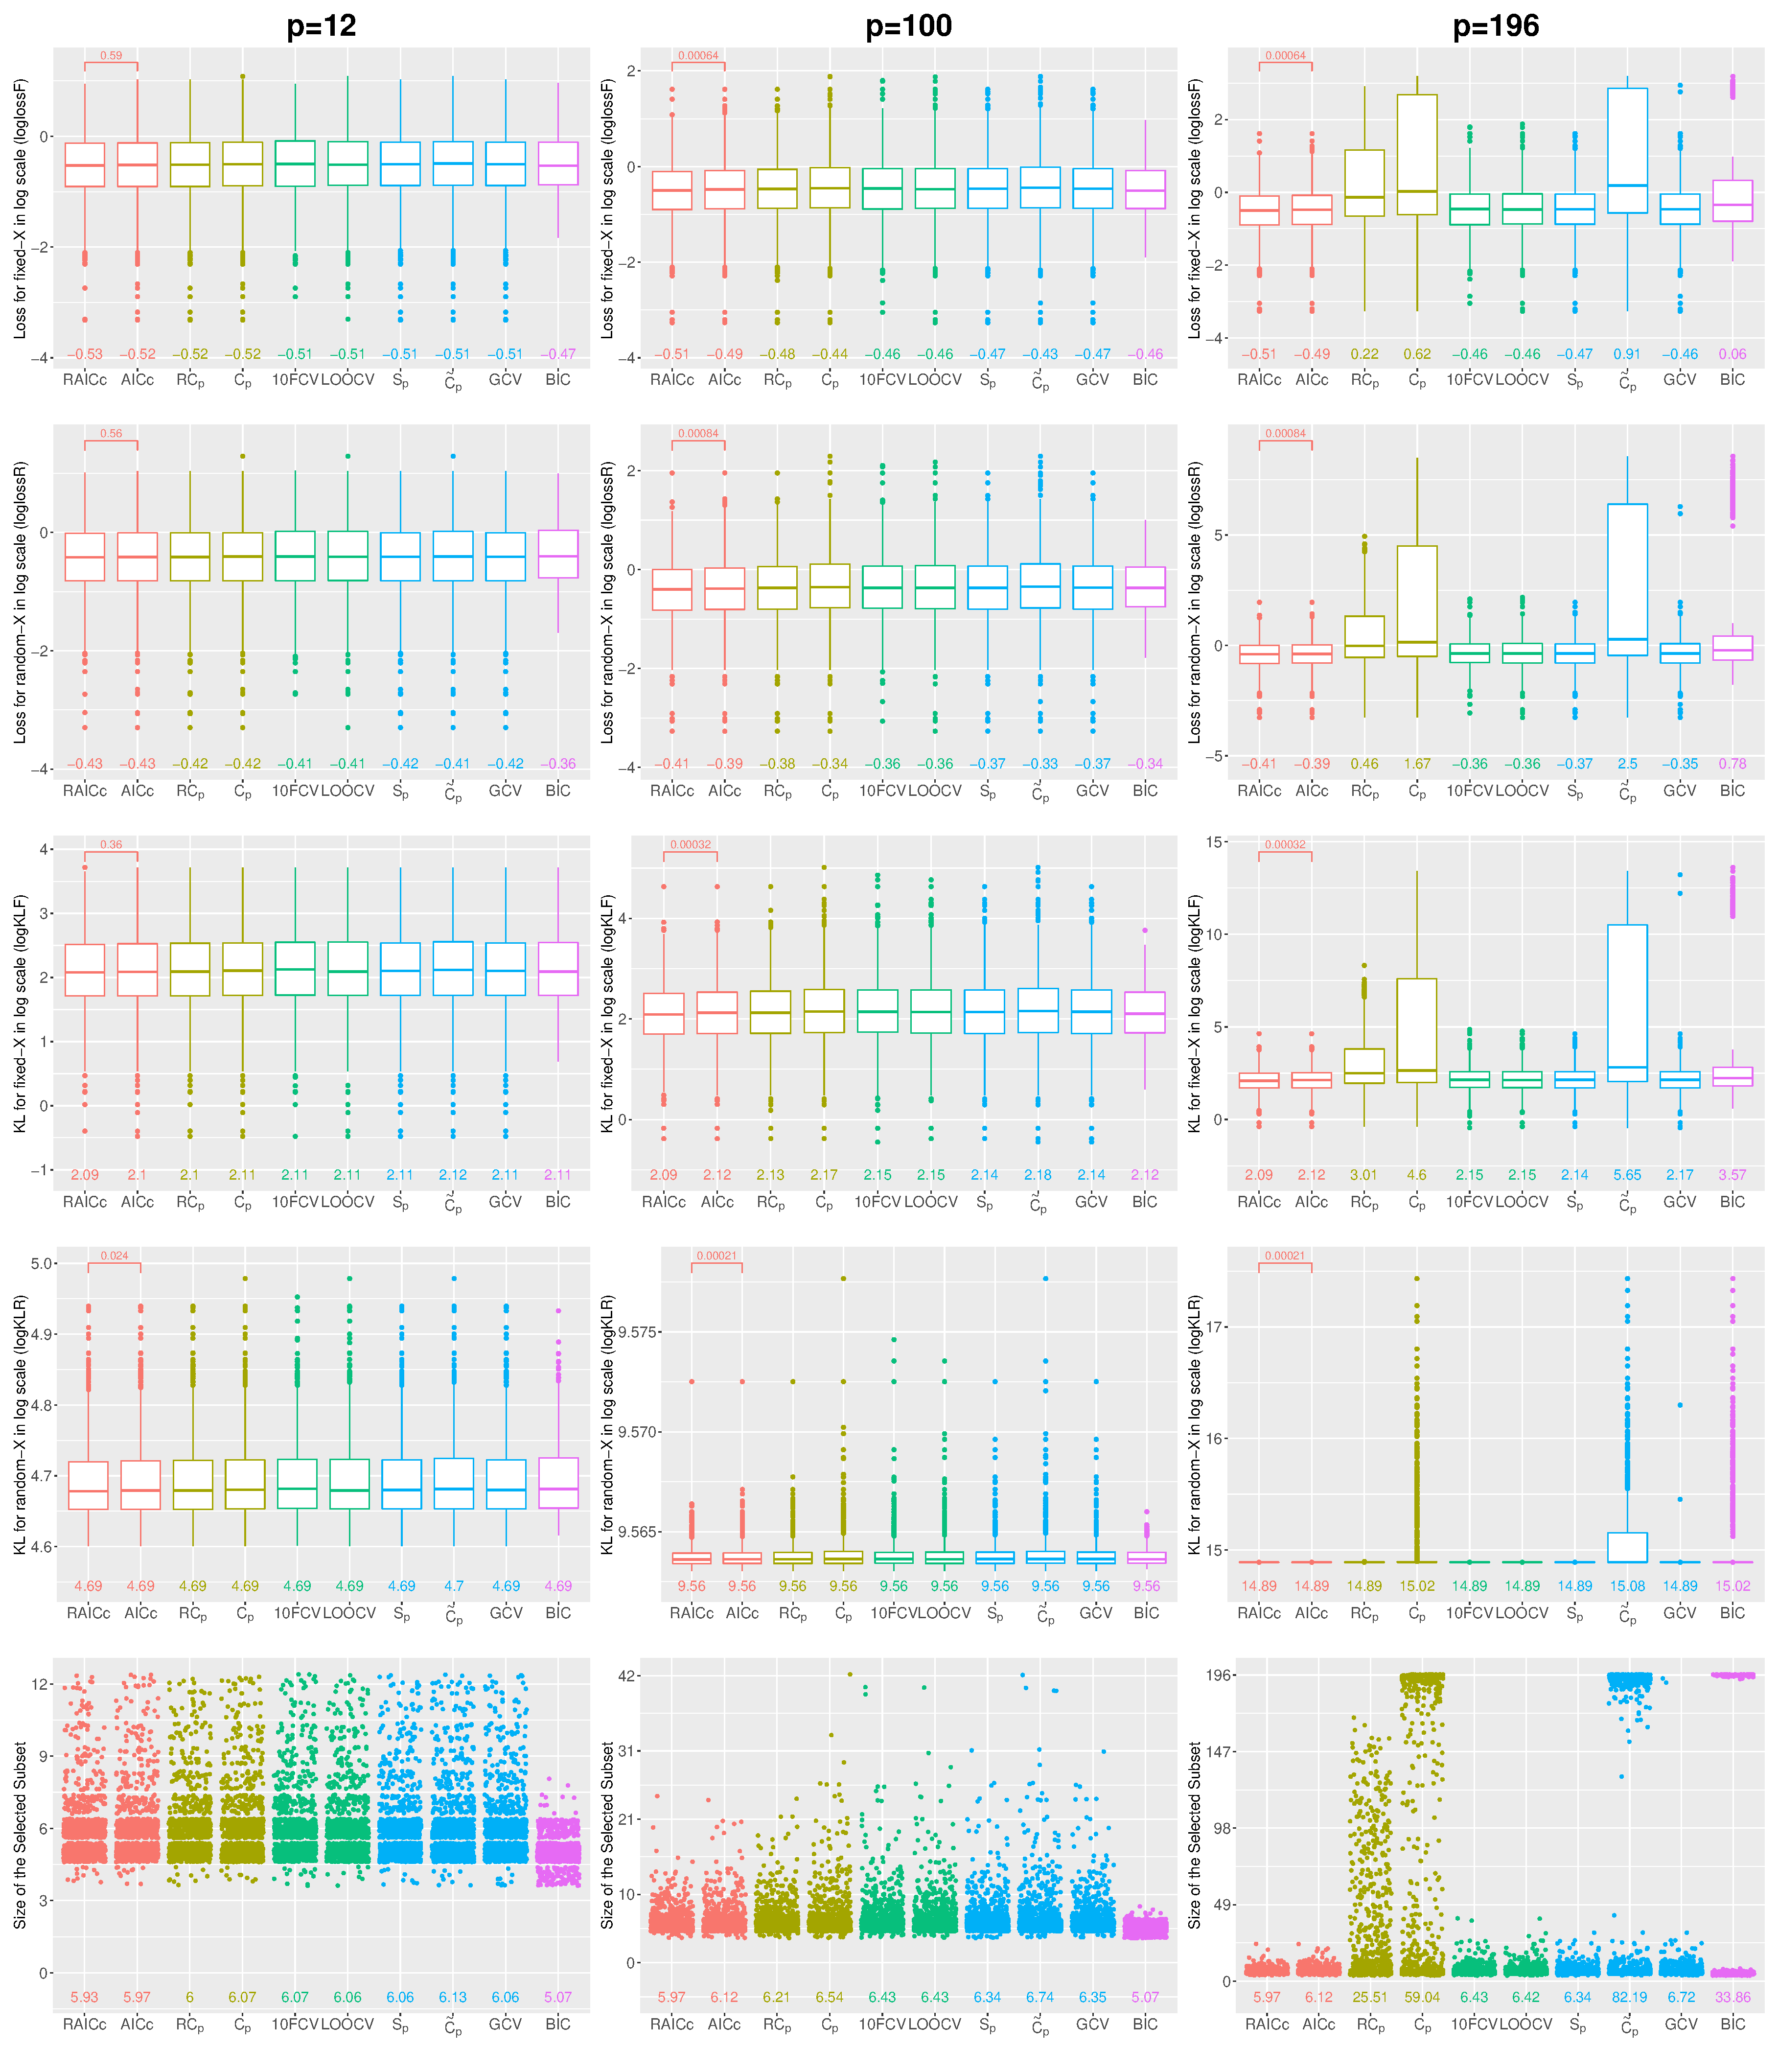
\includegraphics[width=\textwidth]{figures/supplement/fixedx/subset_selection/Sparse-Ex1_n200_hsnr_rho09.eps}
\caption{Variable selection, Fixed-X, Sparse-Ex1, $n=200$, high signal, and $\rho=0.9$.}
\end{figure}
\clearpage
\begin{figure}[!ht]
\centering
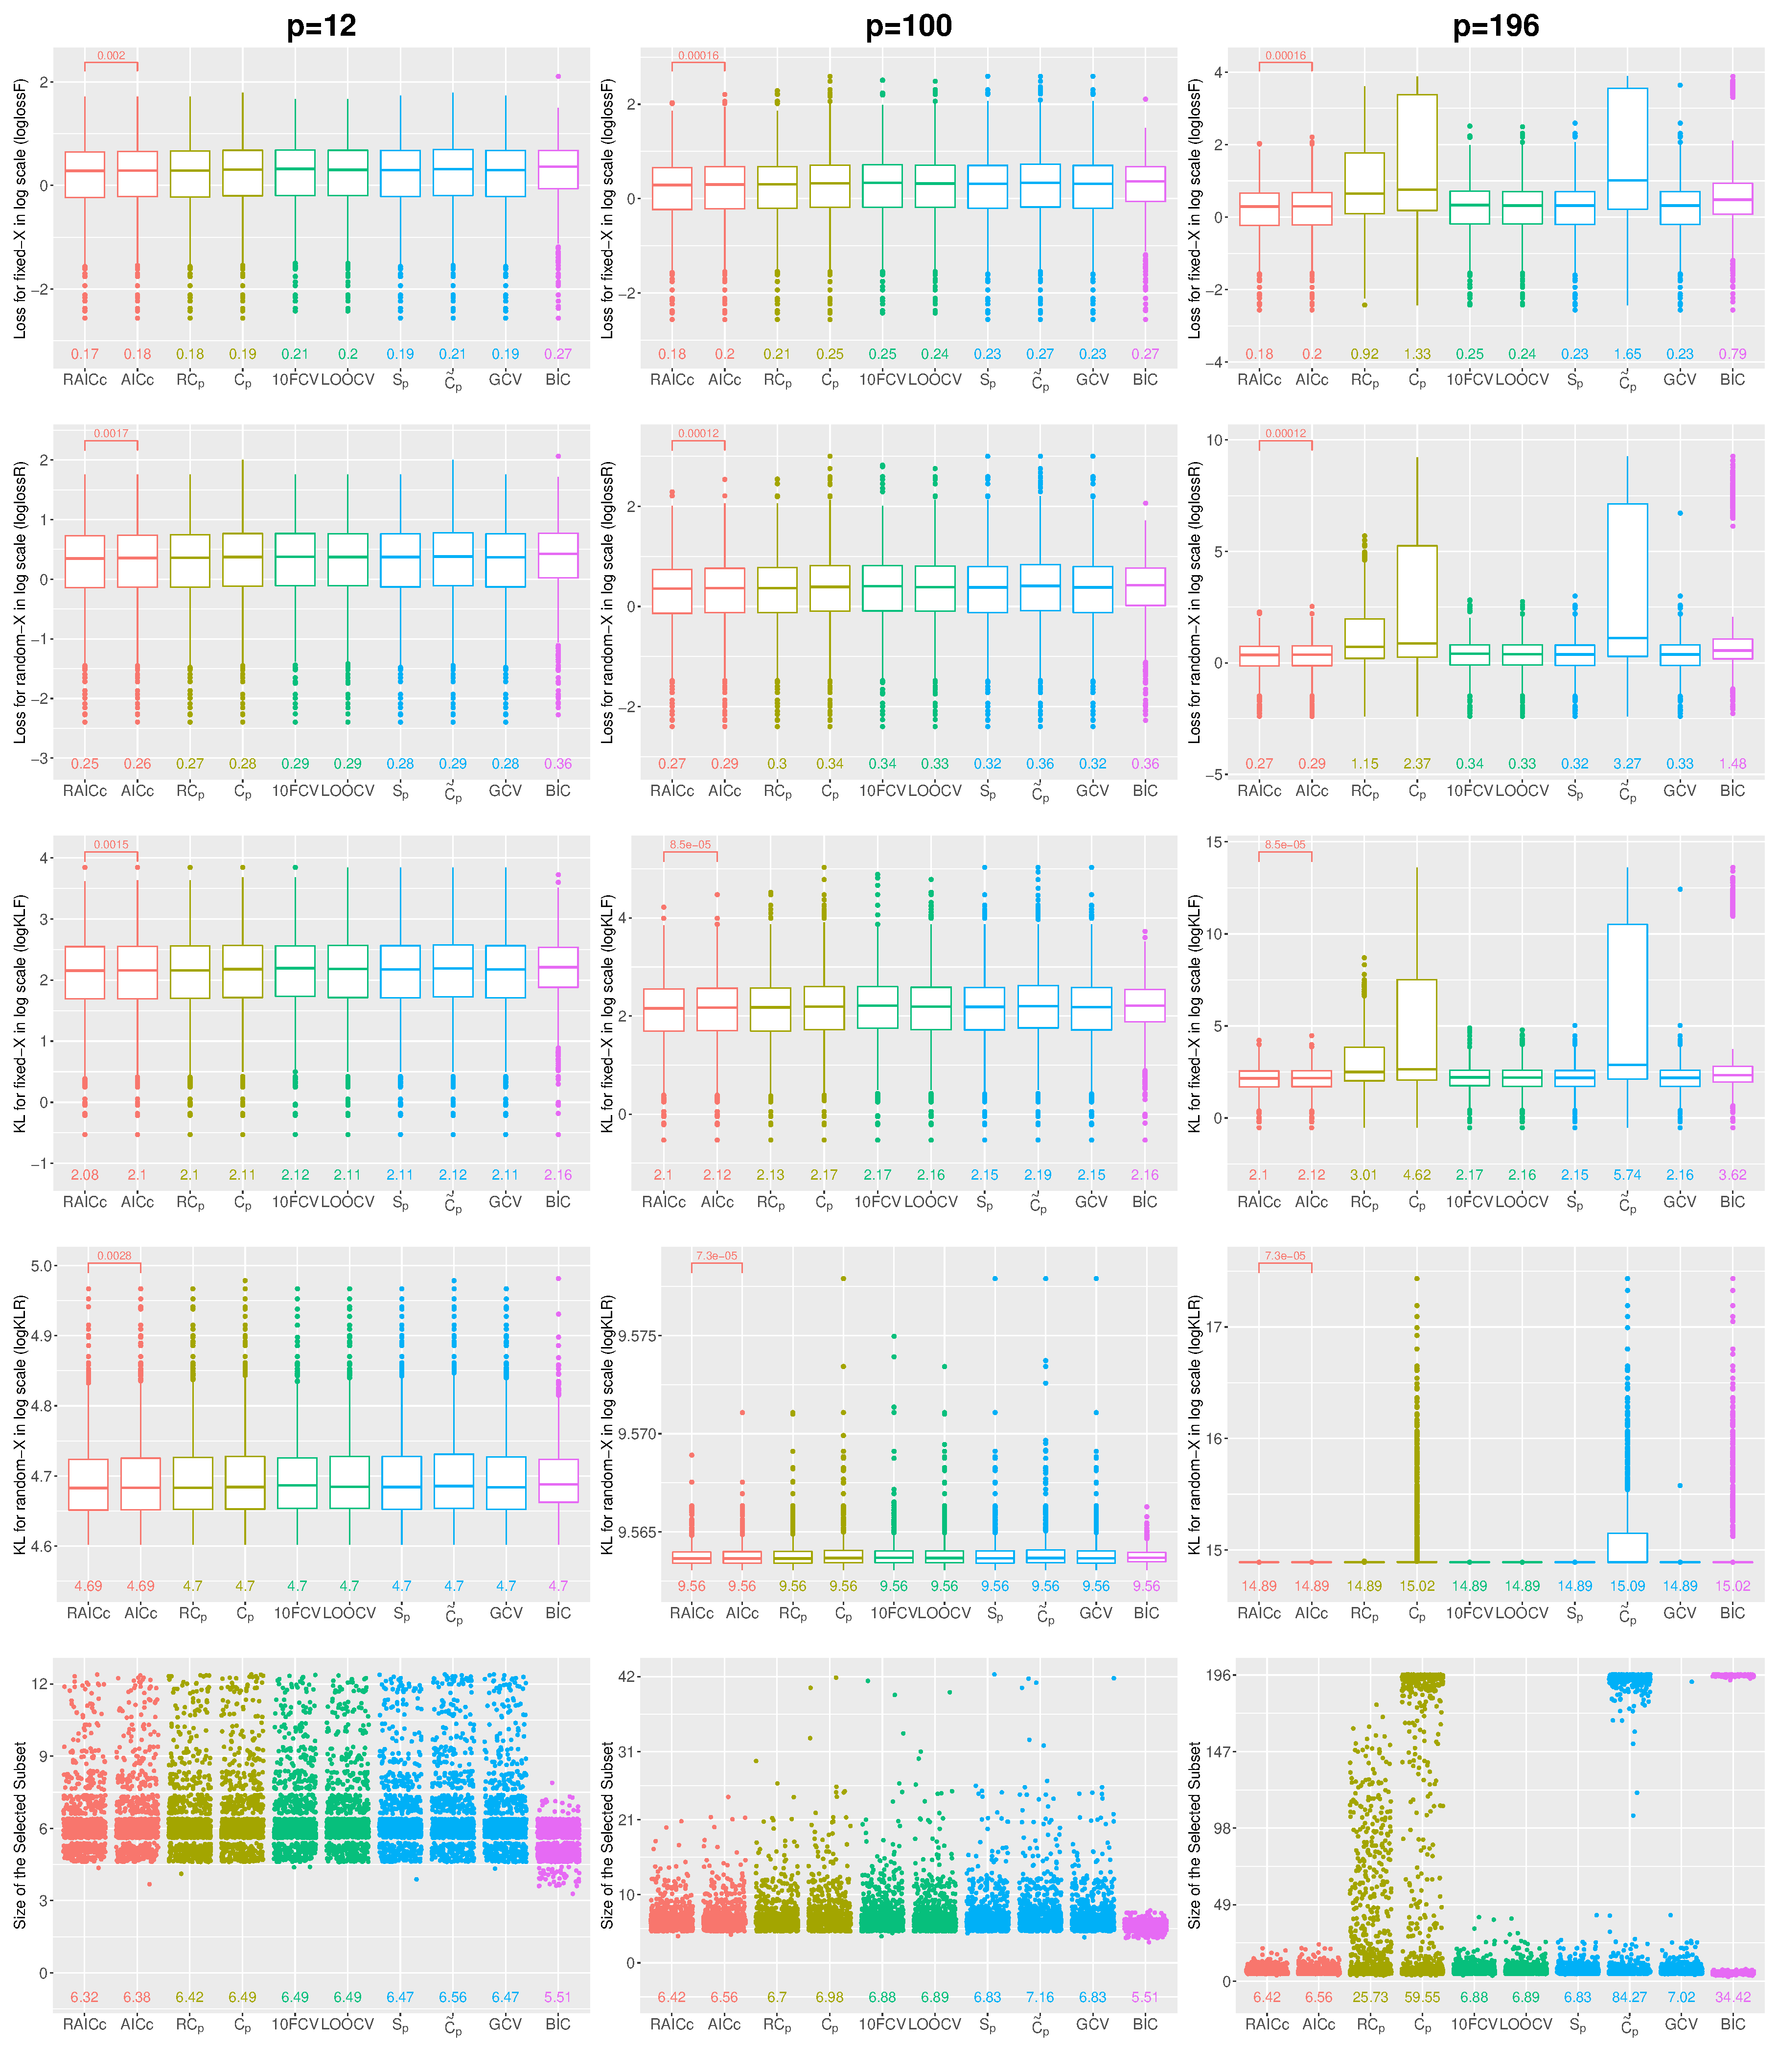
\includegraphics[width=\textwidth]{figures/supplement/fixedx/subset_selection/Sparse-Ex1_n200_msnr_rho0.eps}
\caption{Variable selection, Fixed-X, Sparse-Ex1, $n=200$, medium signal, and $\rho=0$.}
\end{figure}
\clearpage
\begin{figure}[!ht]
\centering
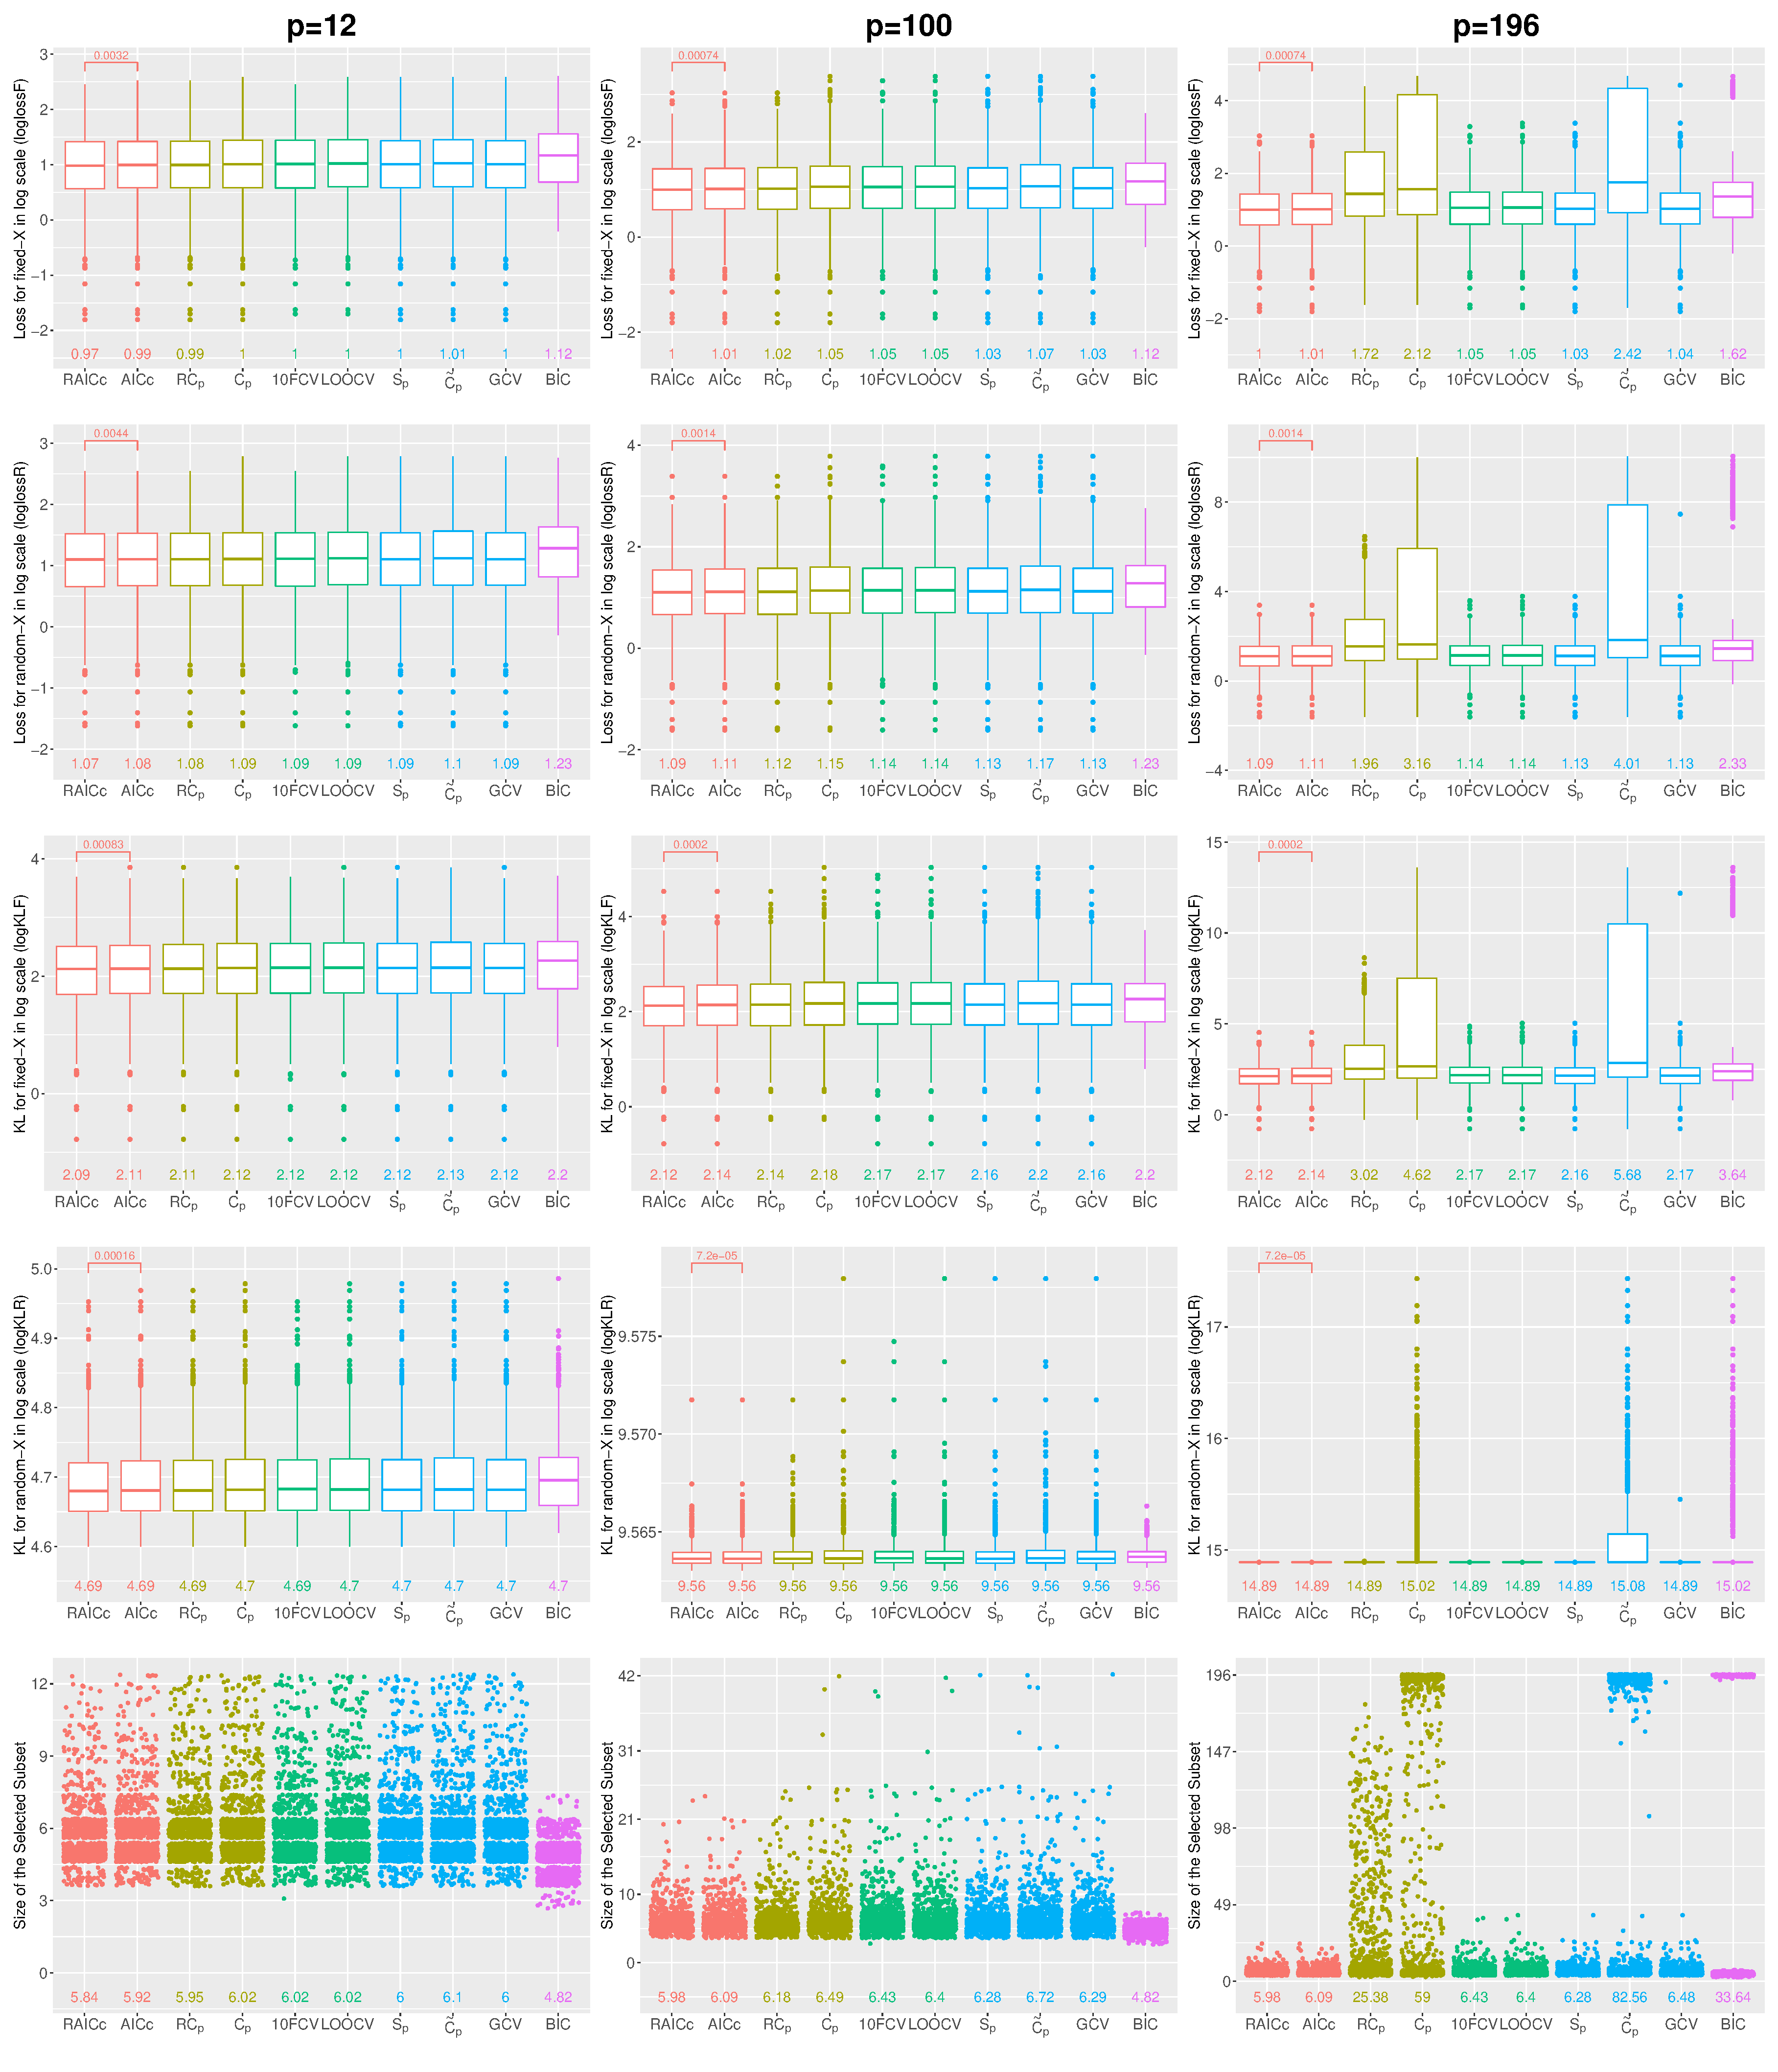
\includegraphics[width=\textwidth]{figures/supplement/fixedx/subset_selection/Sparse-Ex1_n200_msnr_rho05.eps}
\caption{Variable selection, Fixed-X, Sparse-Ex1, $n=200$, medium signal, and $\rho=0.5$.}
\end{figure}
\clearpage
\begin{figure}[!ht]
\centering
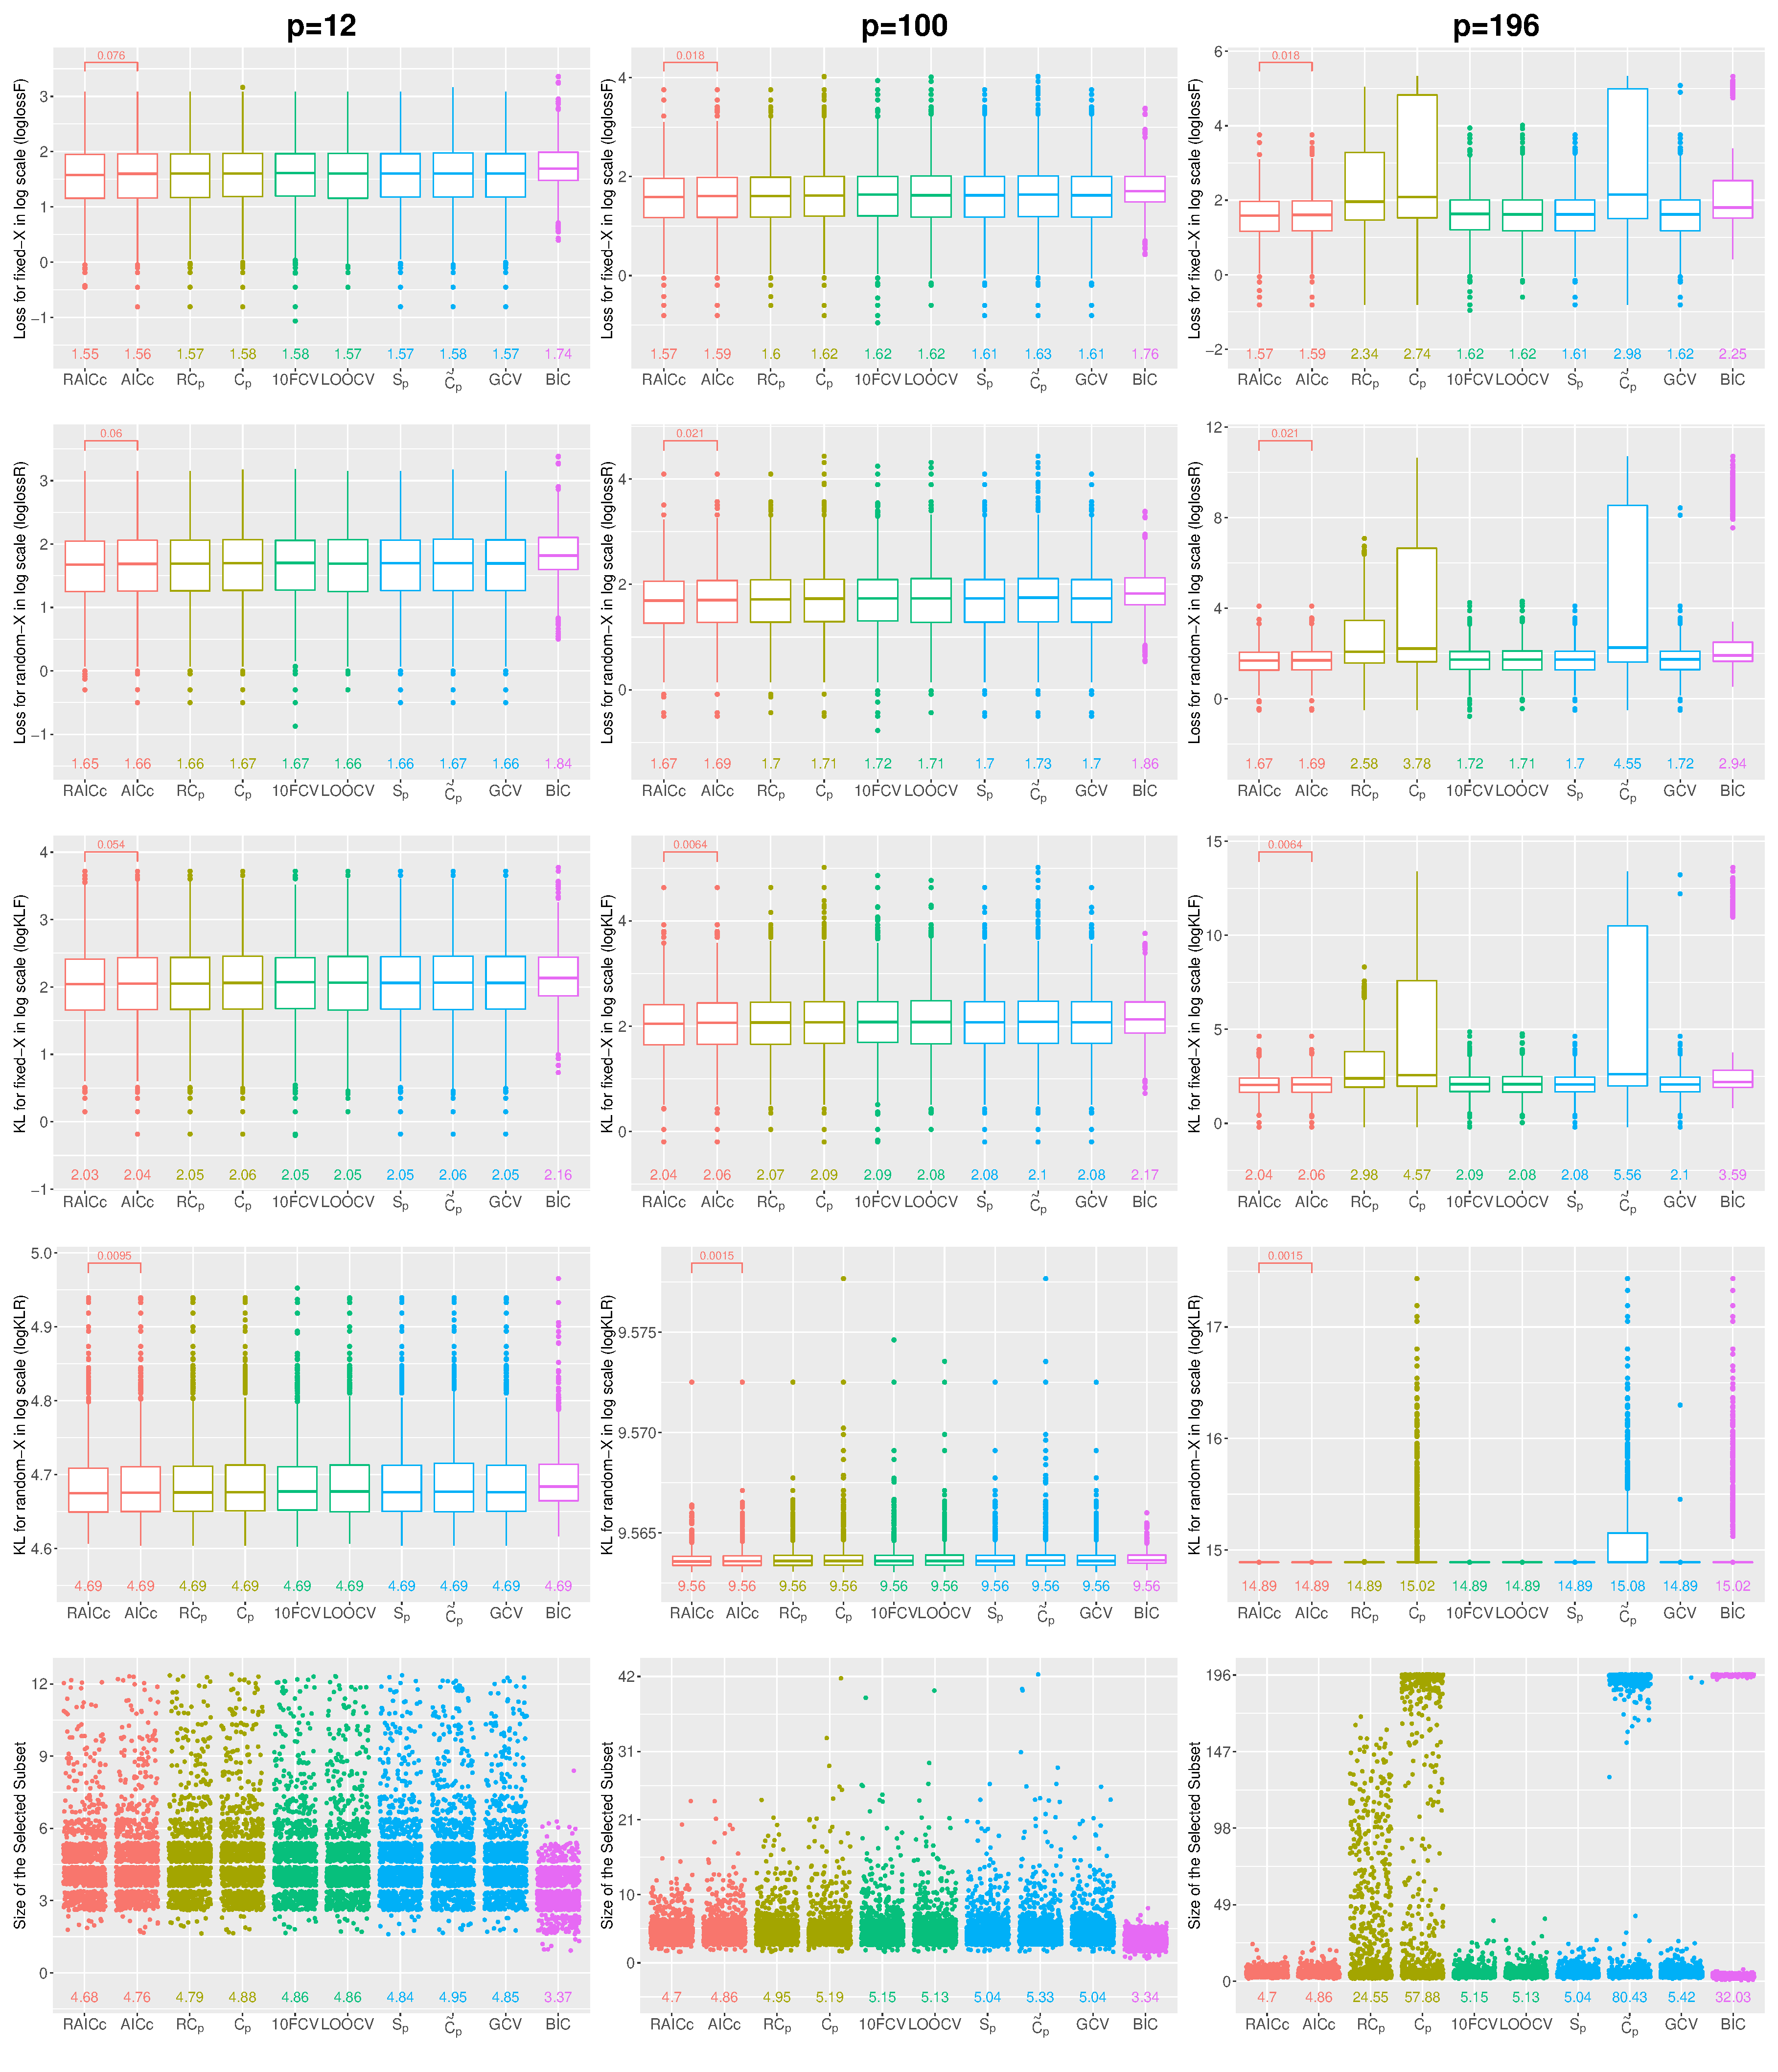
\includegraphics[width=\textwidth]{figures/supplement/fixedx/subset_selection/Sparse-Ex1_n200_msnr_rho09.eps}
\caption{Variable selection, Fixed-X, Sparse-Ex1, $n=200$, medium signal, and $\rho=0.9$.}
\end{figure}
\clearpage
\begin{figure}[!ht]
\centering
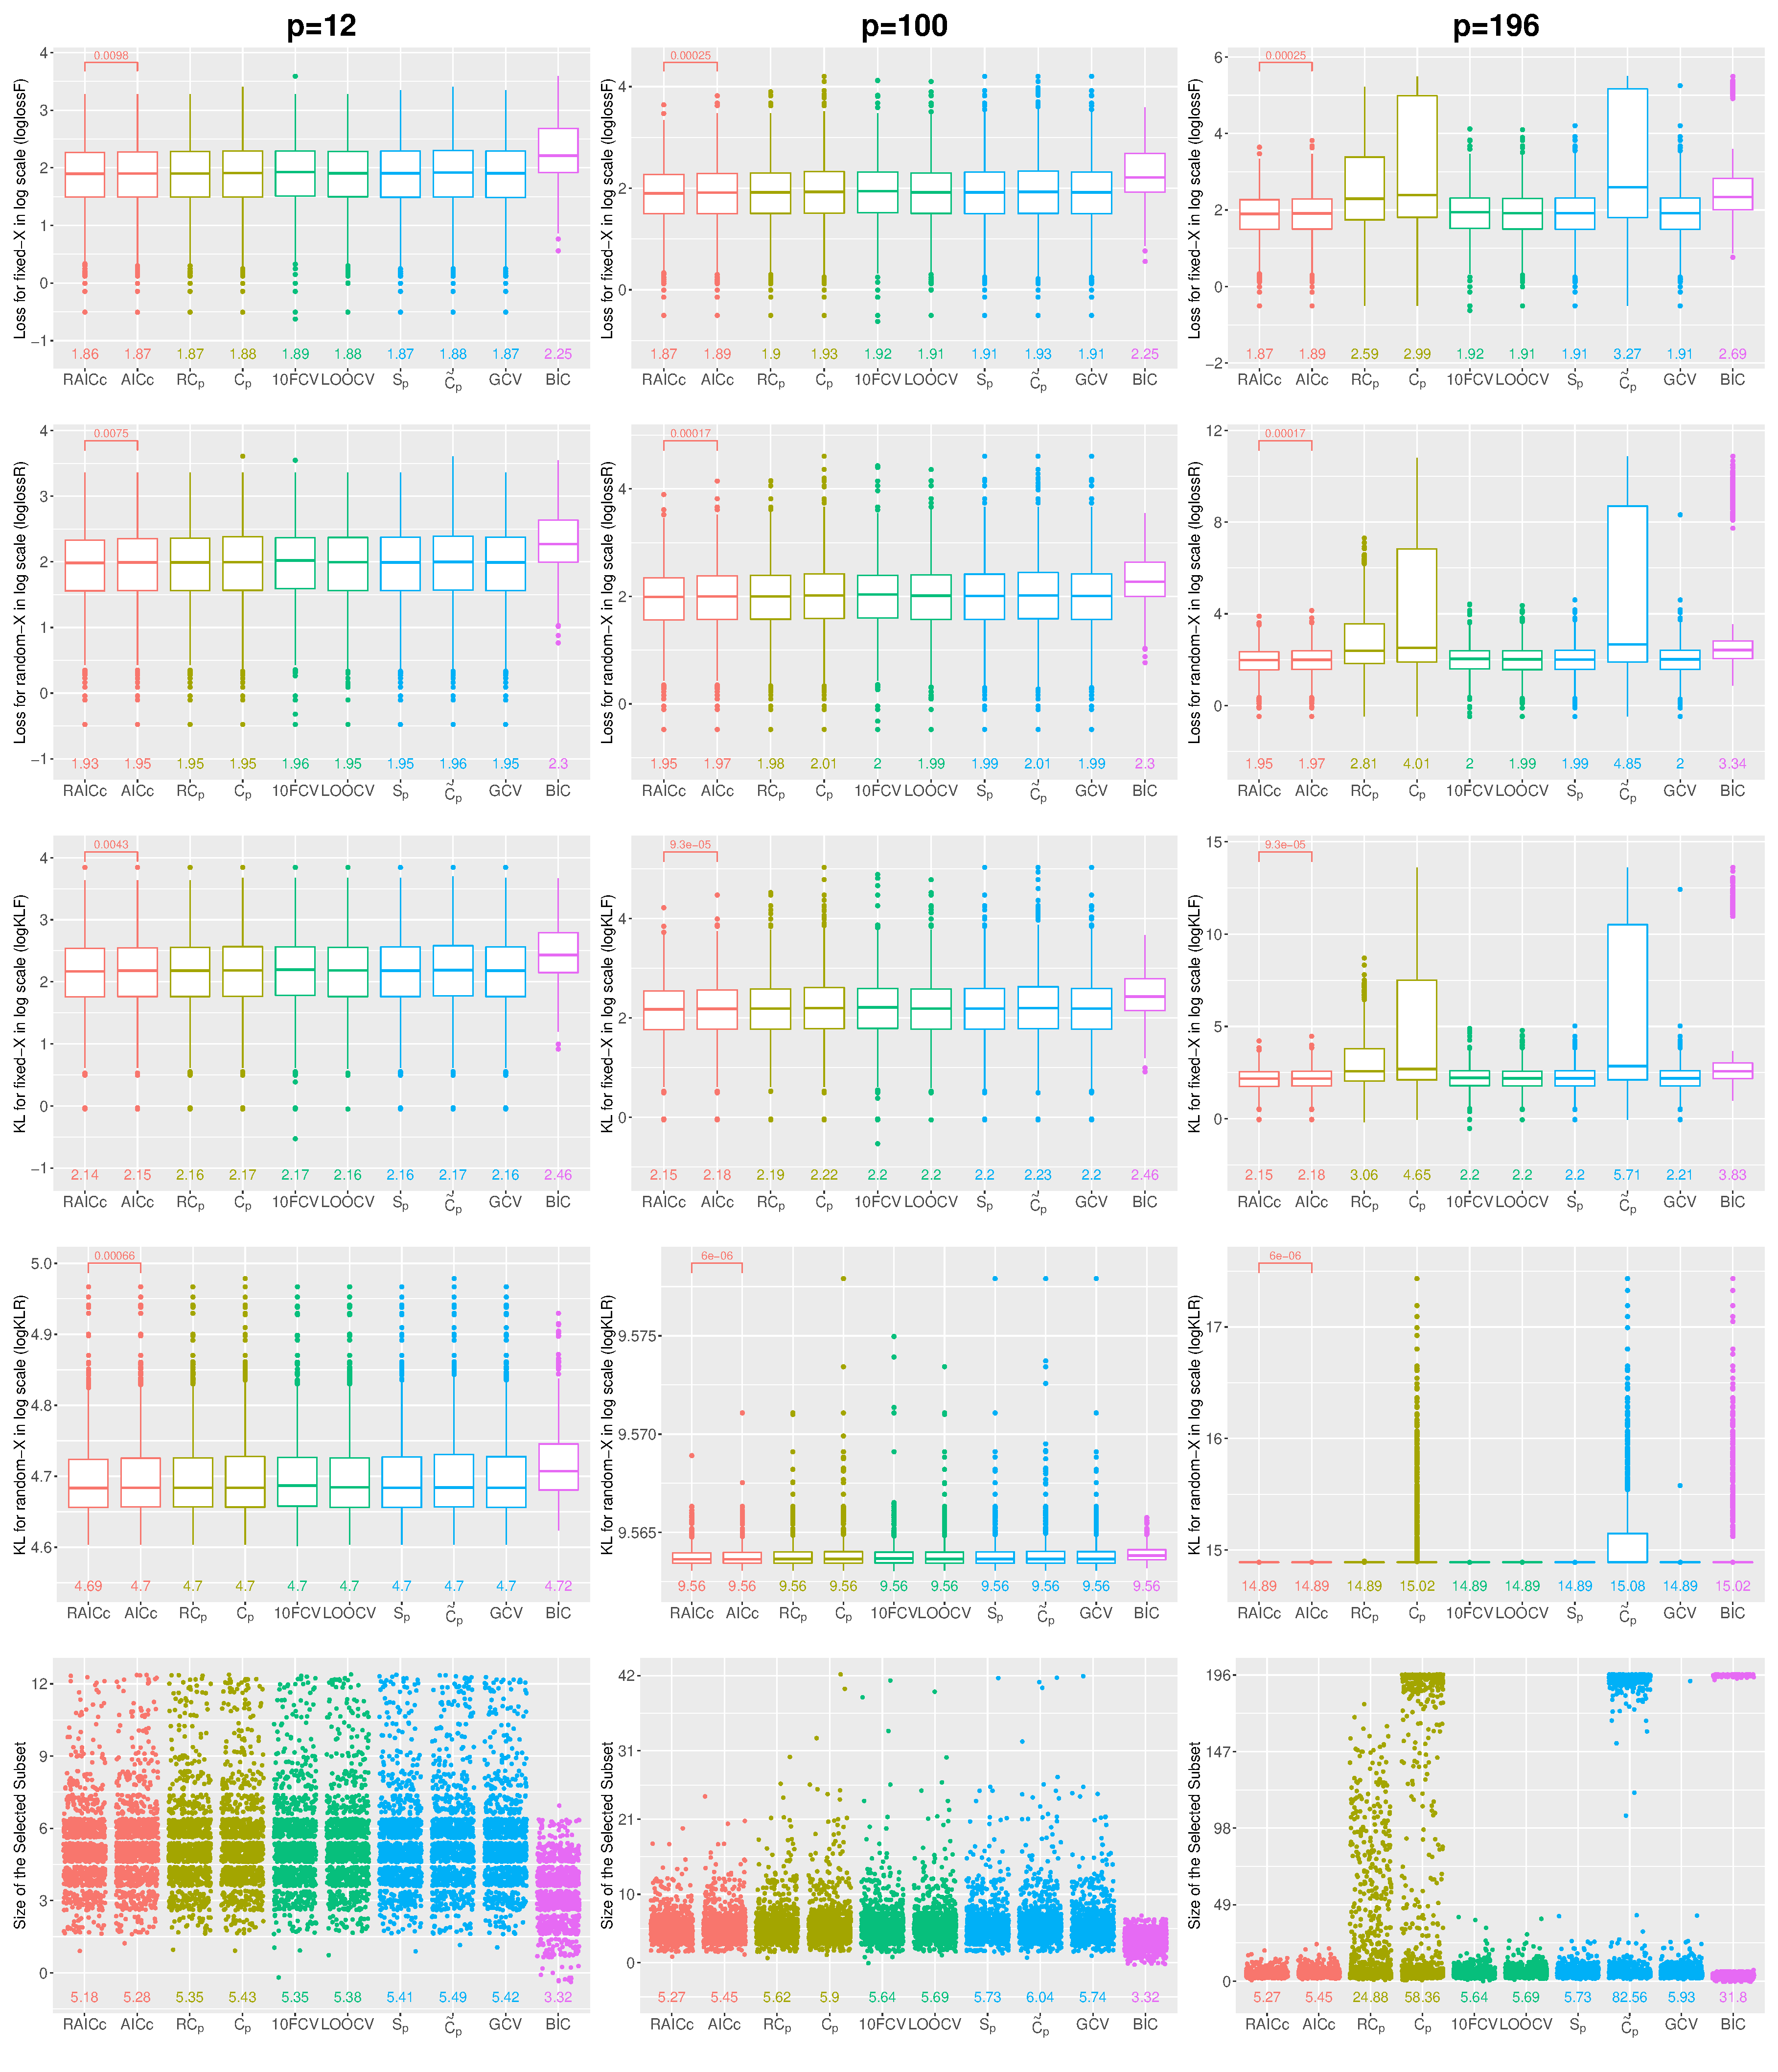
\includegraphics[width=\textwidth]{figures/supplement/fixedx/subset_selection/Sparse-Ex1_n200_lsnr_rho0.eps}
\caption{Variable selection, Fixed-X, Sparse-Ex1, $n=200$, low signal, and $\rho=0$.}
\end{figure}
\clearpage
\begin{figure}[!ht]
\centering
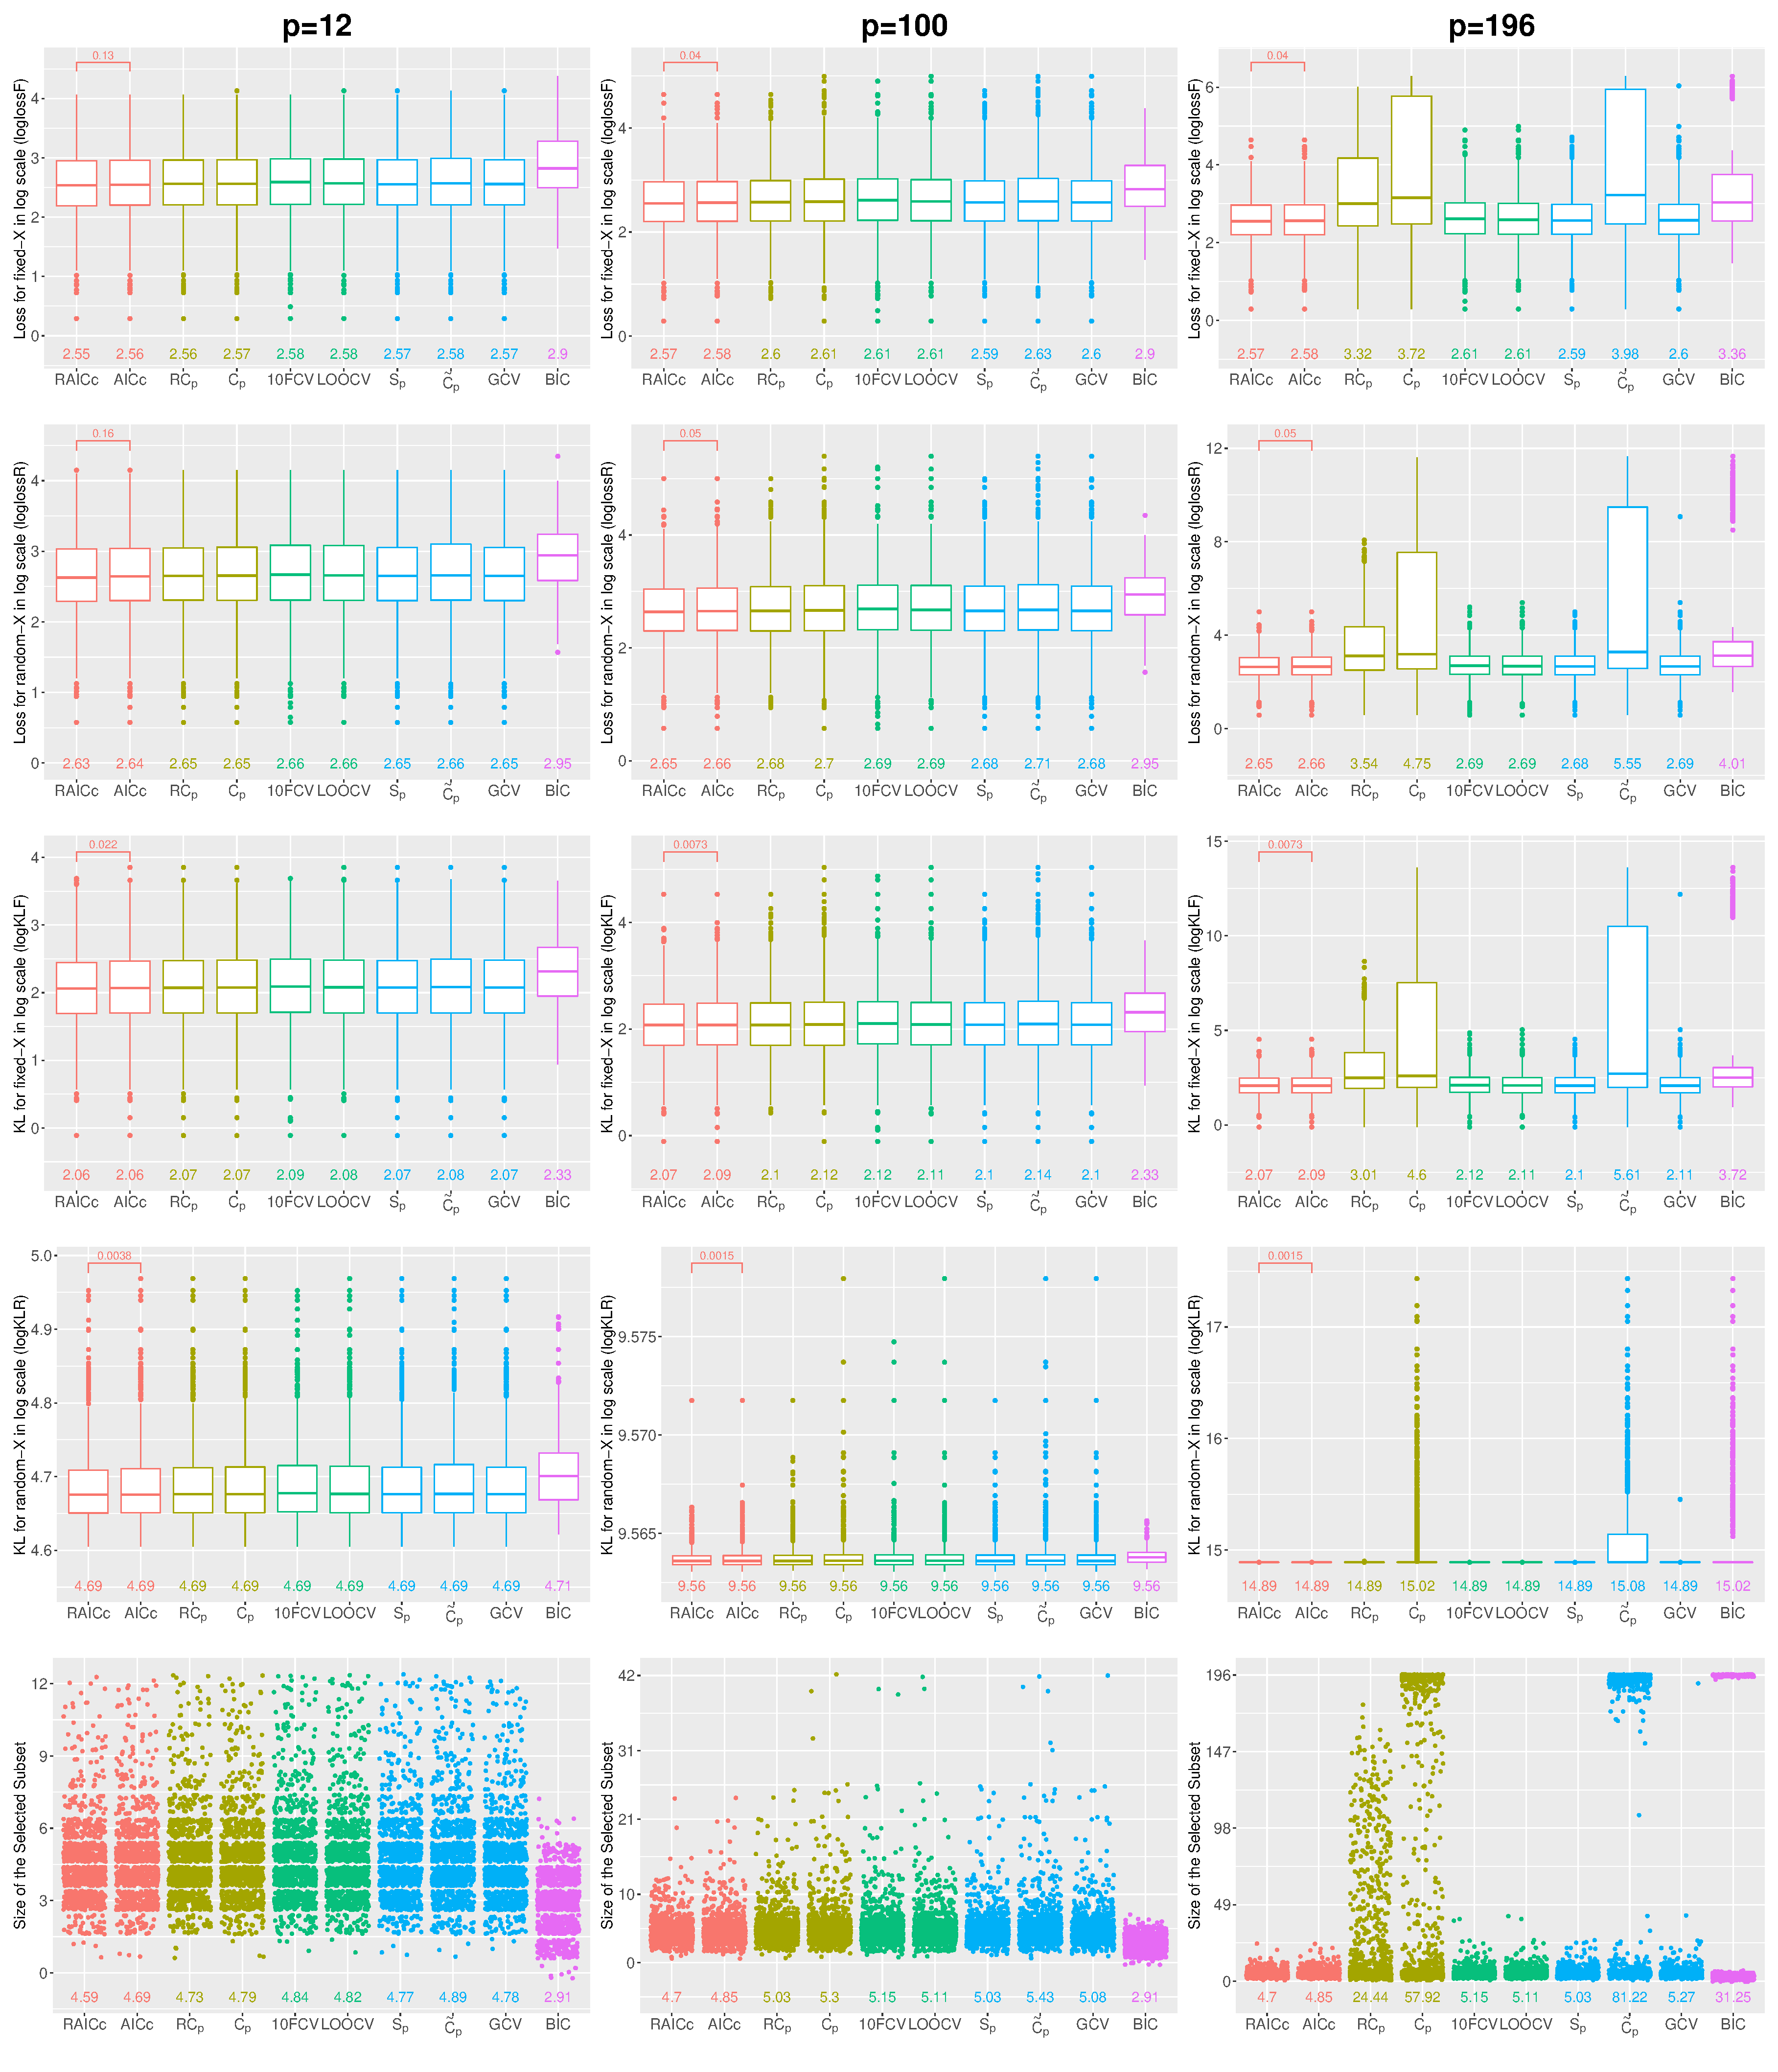
\includegraphics[width=\textwidth]{figures/supplement/fixedx/subset_selection/Sparse-Ex1_n200_lsnr_rho05.eps}
\caption{Variable selection, Fixed-X, Sparse-Ex1, $n=200$, low signal, and $\rho=0.5$.}
\end{figure}
\clearpage
\begin{figure}[!ht]
\centering
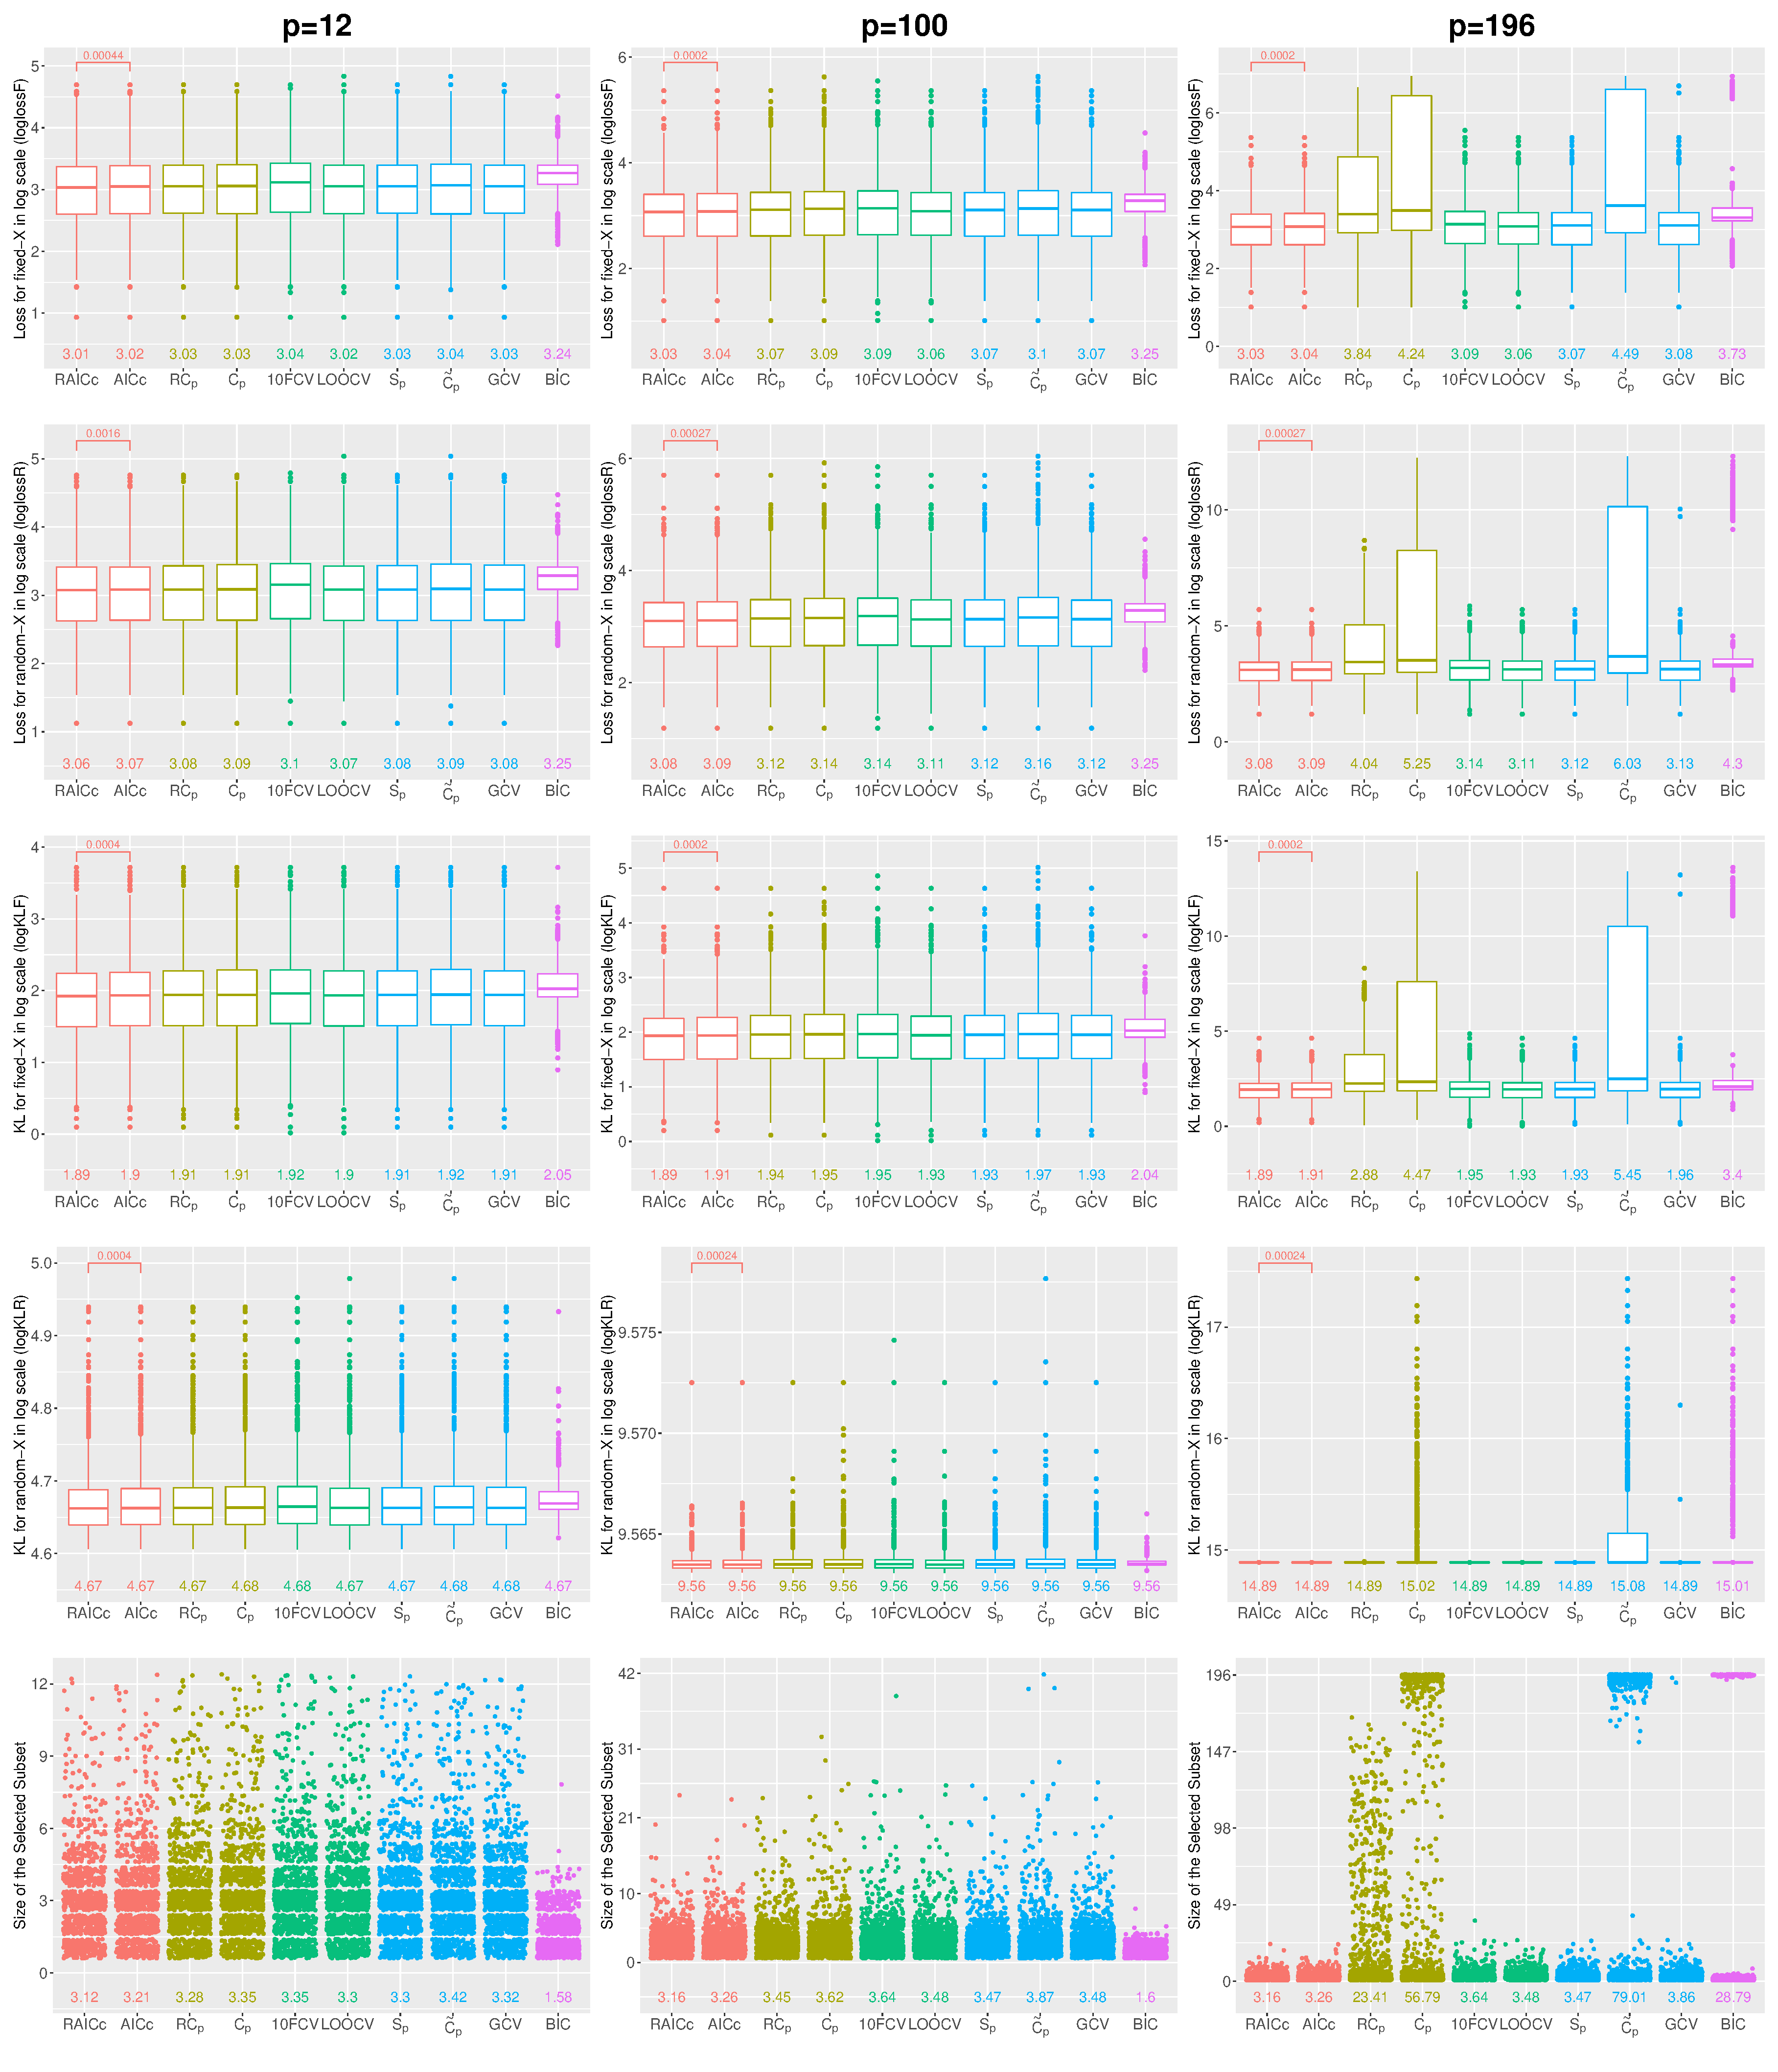
\includegraphics[width=\textwidth]{figures/supplement/fixedx/subset_selection/Sparse-Ex1_n200_lsnr_rho09.eps}
\caption{Variable selection, Fixed-X, Sparse-Ex1, $n=200$, low signal, and $\rho=0.9$.}
\end{figure}
\clearpage
\begin{figure}[!ht]
\centering
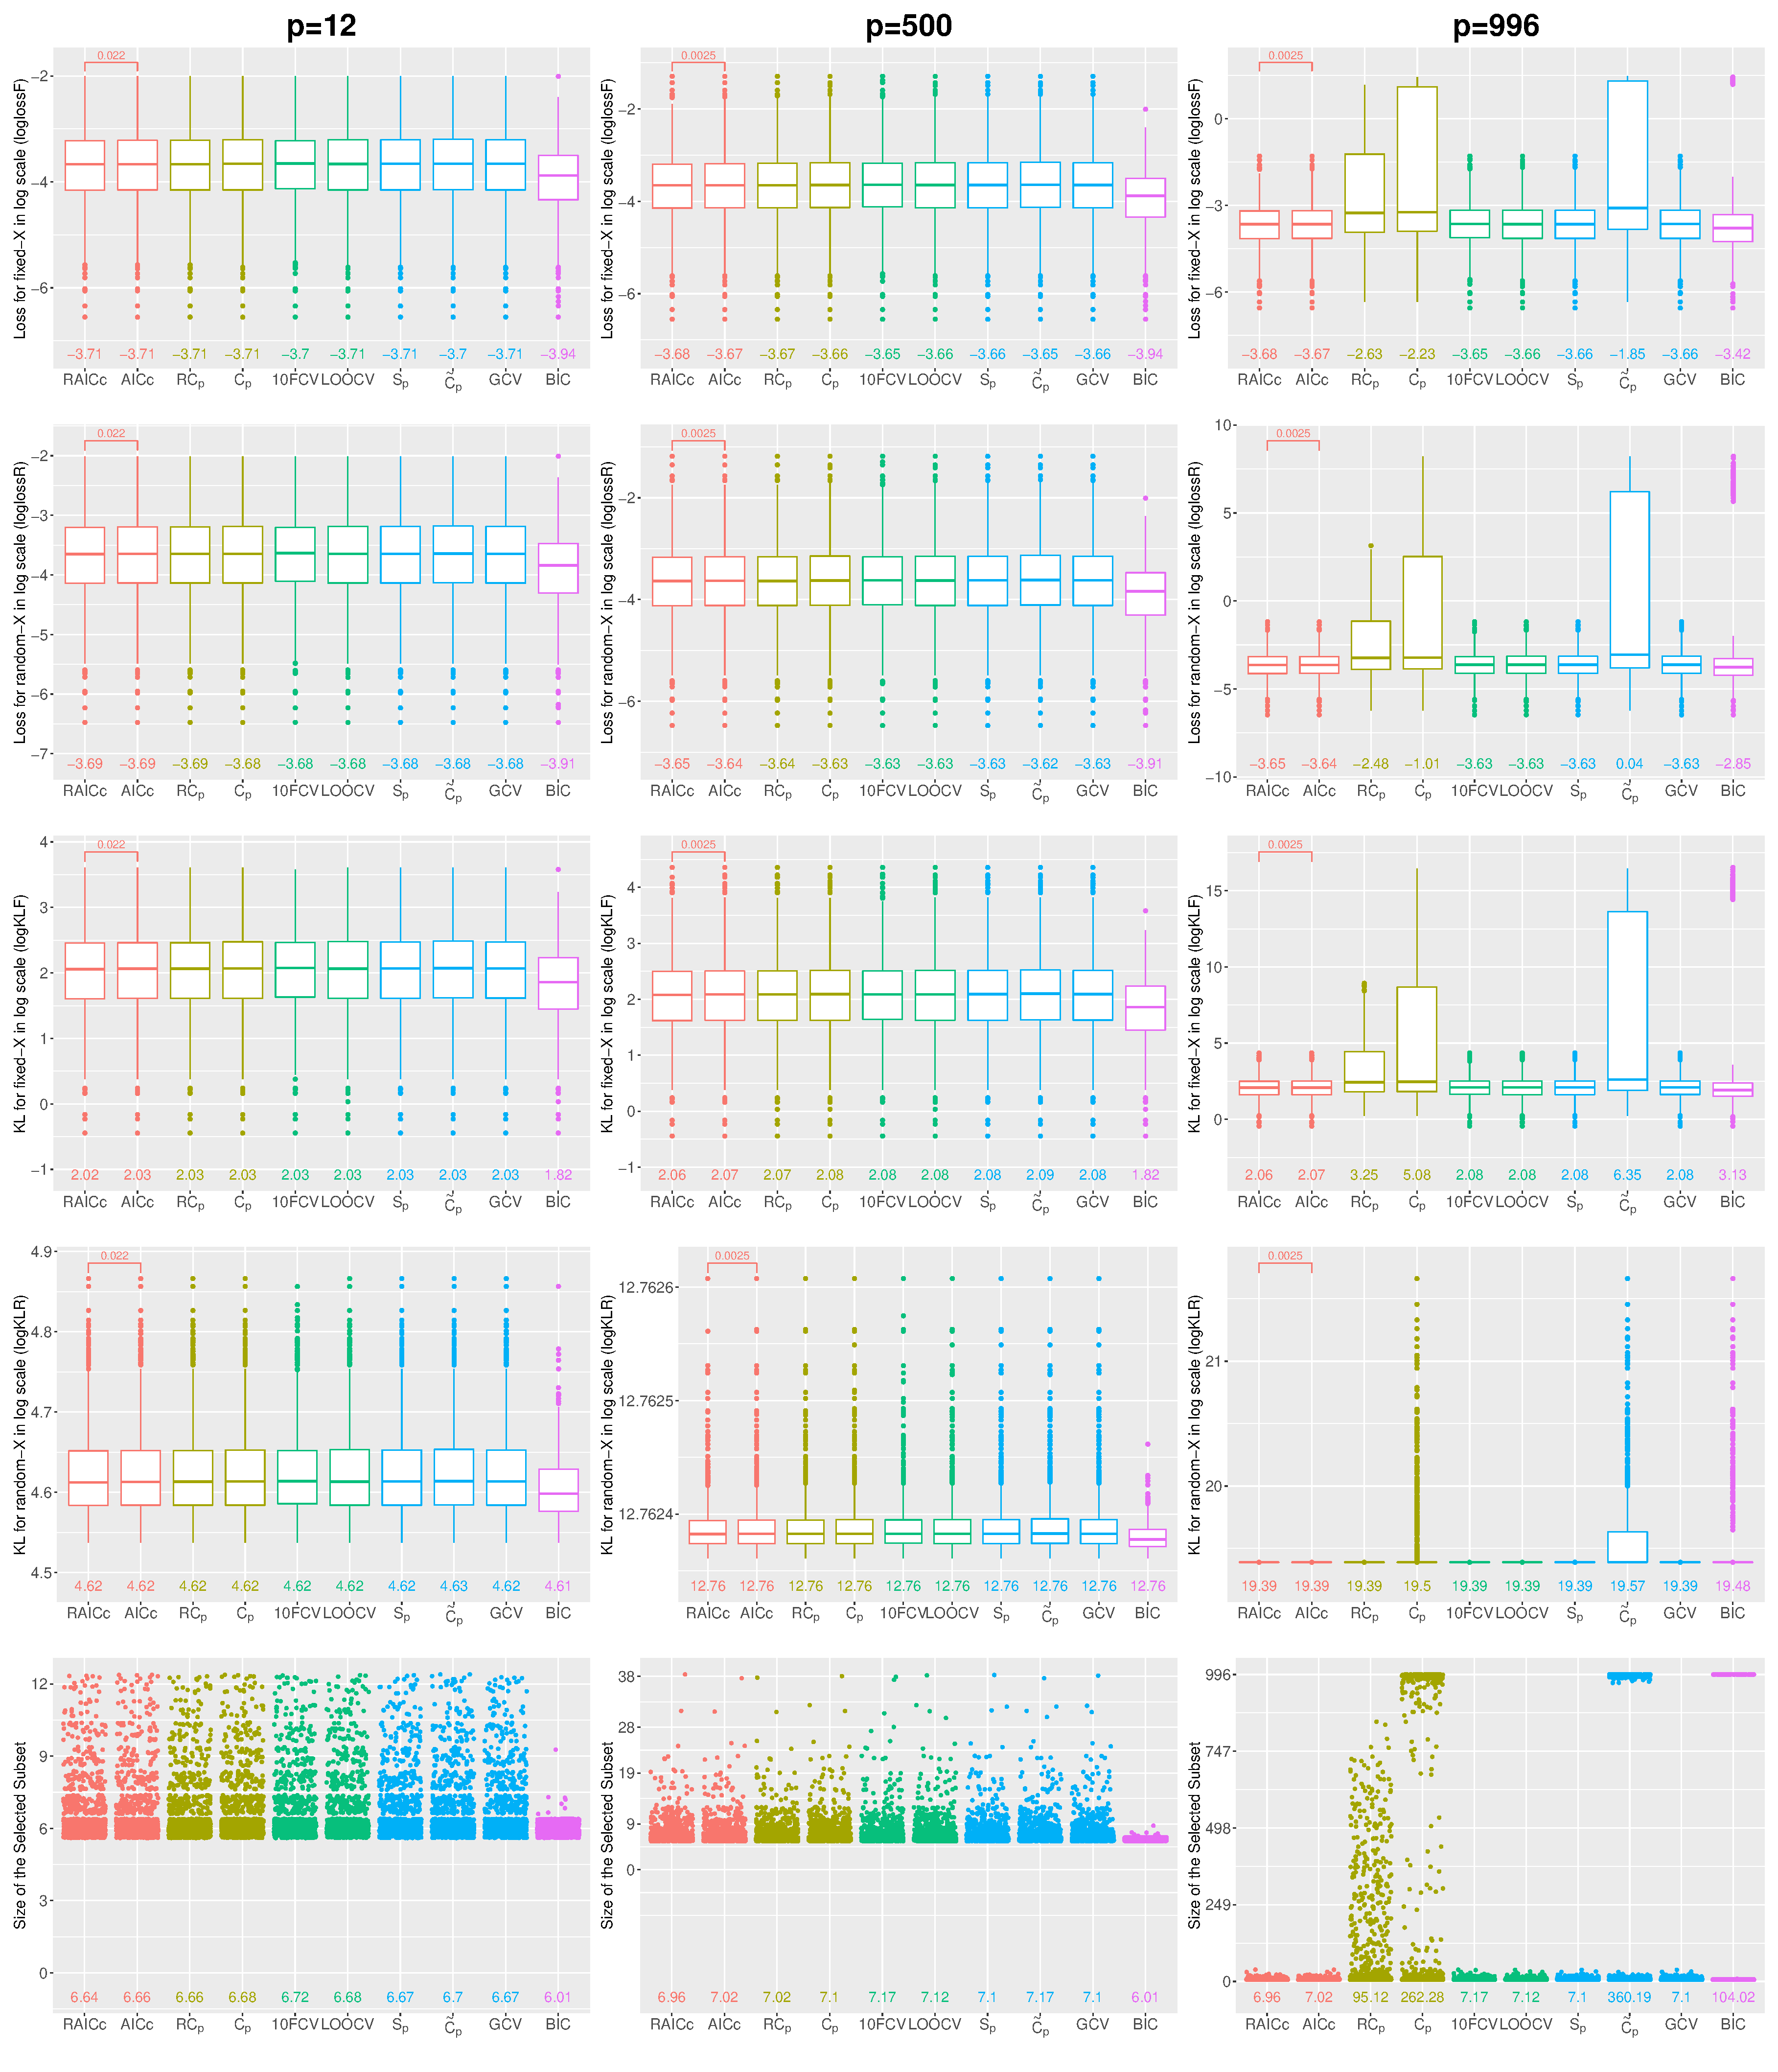
\includegraphics[width=\textwidth]{figures/supplement/fixedx/subset_selection/Sparse-Ex1_n1000_hsnr_rho0.eps}
\caption{Variable selection, Fixed-X, Sparse-Ex1, $n=1000$, high signal, and $\rho=0$.}
\end{figure}
\clearpage
\begin{figure}[!ht]
\centering
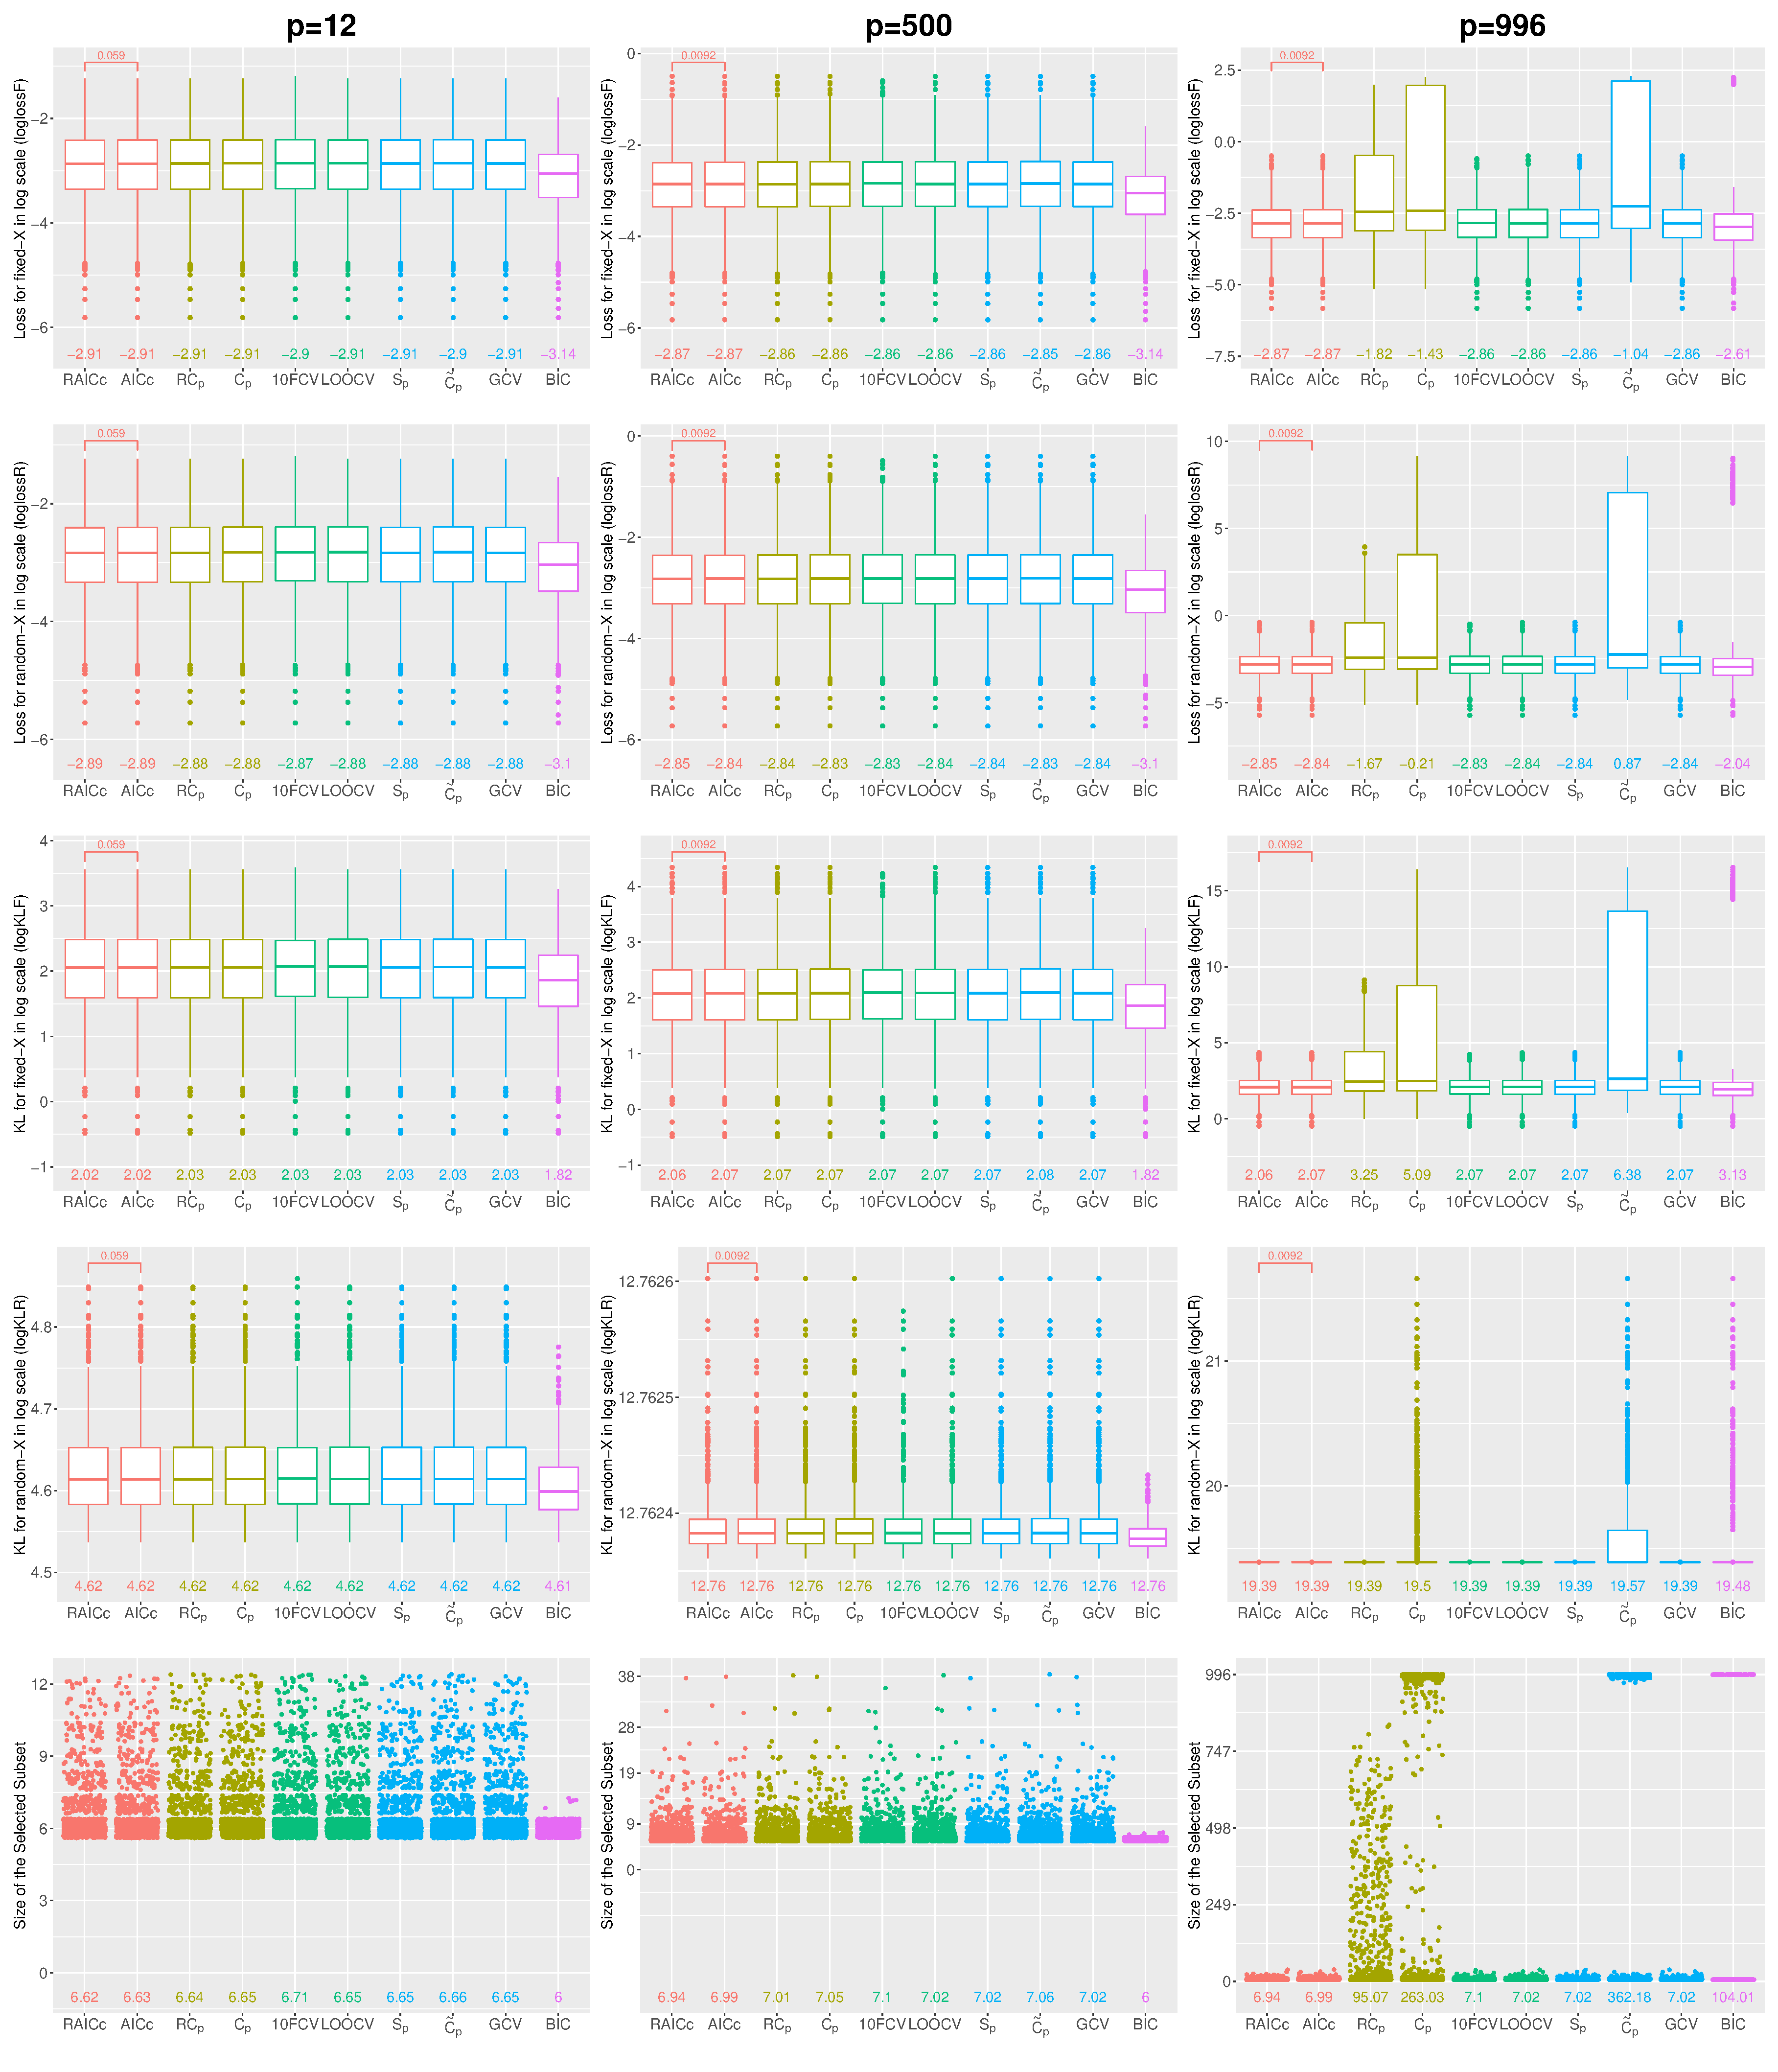
\includegraphics[width=\textwidth]{figures/supplement/fixedx/subset_selection/Sparse-Ex1_n1000_hsnr_rho05.eps}
\caption{Variable selection, Fixed-X, Sparse-Ex1, $n=1000$, high signal, and $\rho=0.5$.}
\end{figure}
\clearpage
\begin{figure}[!ht]
\centering
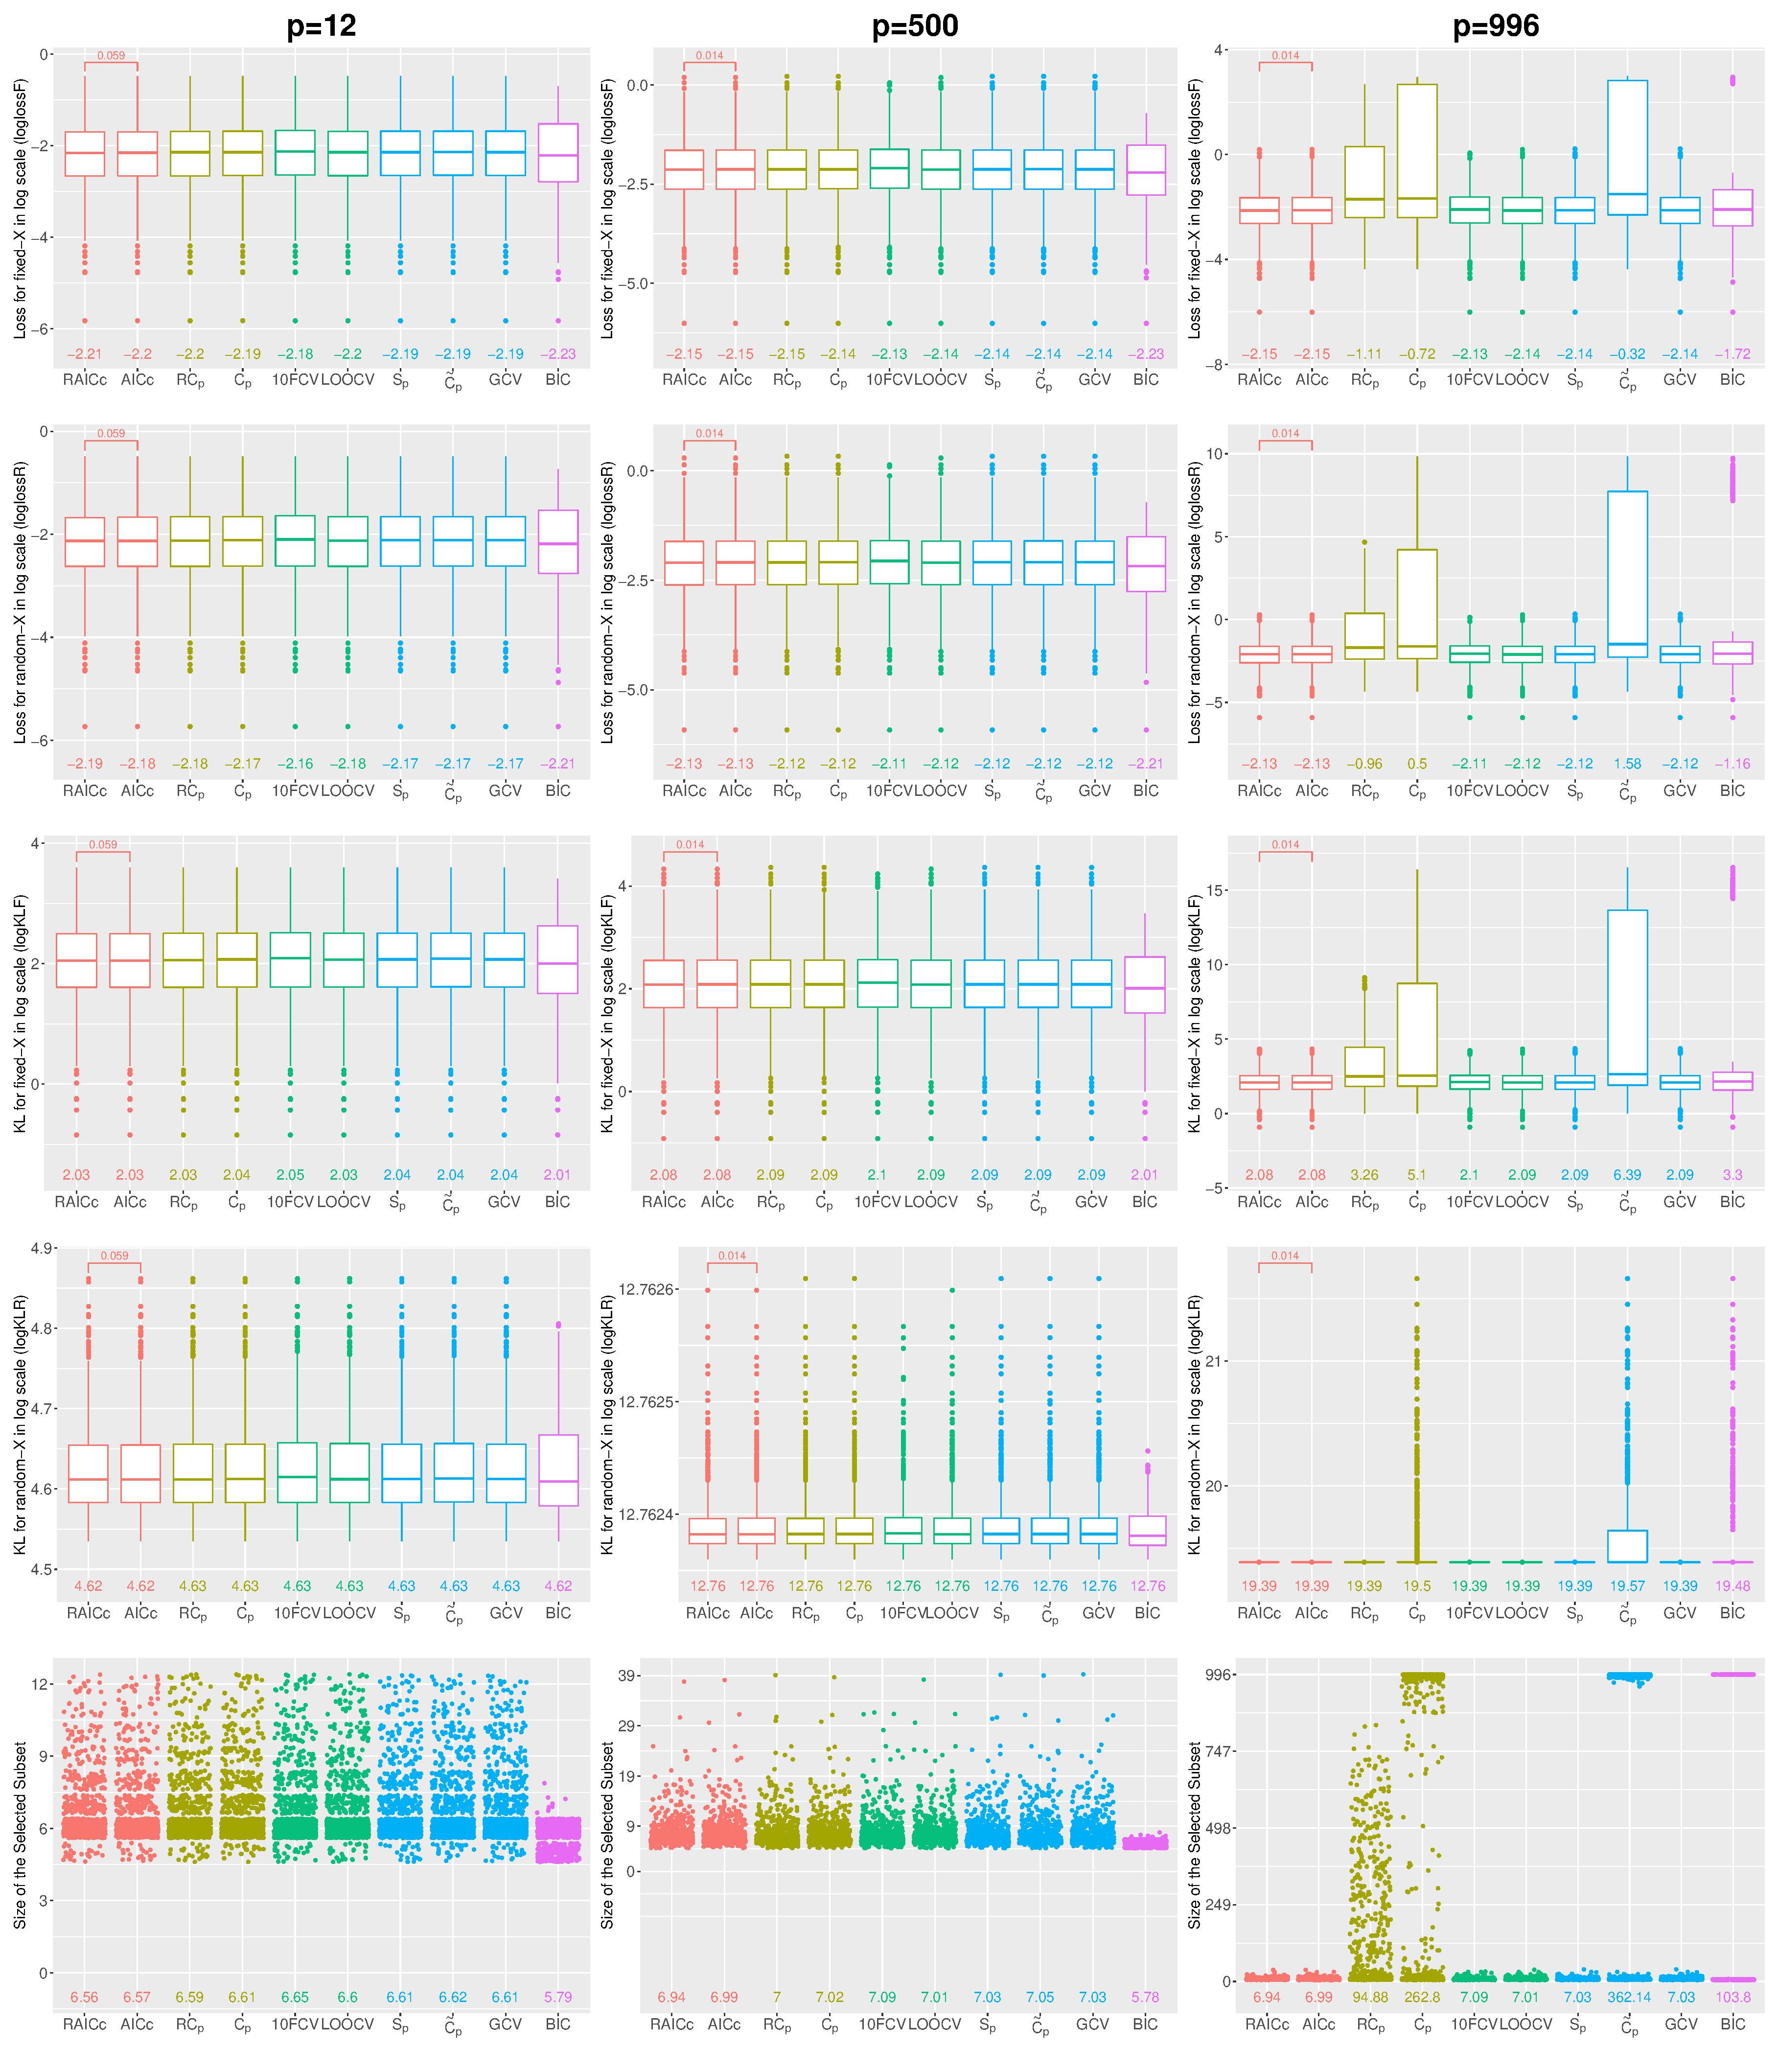
\includegraphics[width=\textwidth]{figures/supplement/fixedx/subset_selection/Sparse-Ex1_n1000_hsnr_rho09.eps}
\caption{Variable selection, Fixed-X, Sparse-Ex1, $n=1000$, high signal, and $\rho=0.9$.}
\end{figure}
\clearpage
\begin{figure}[!ht]
\centering
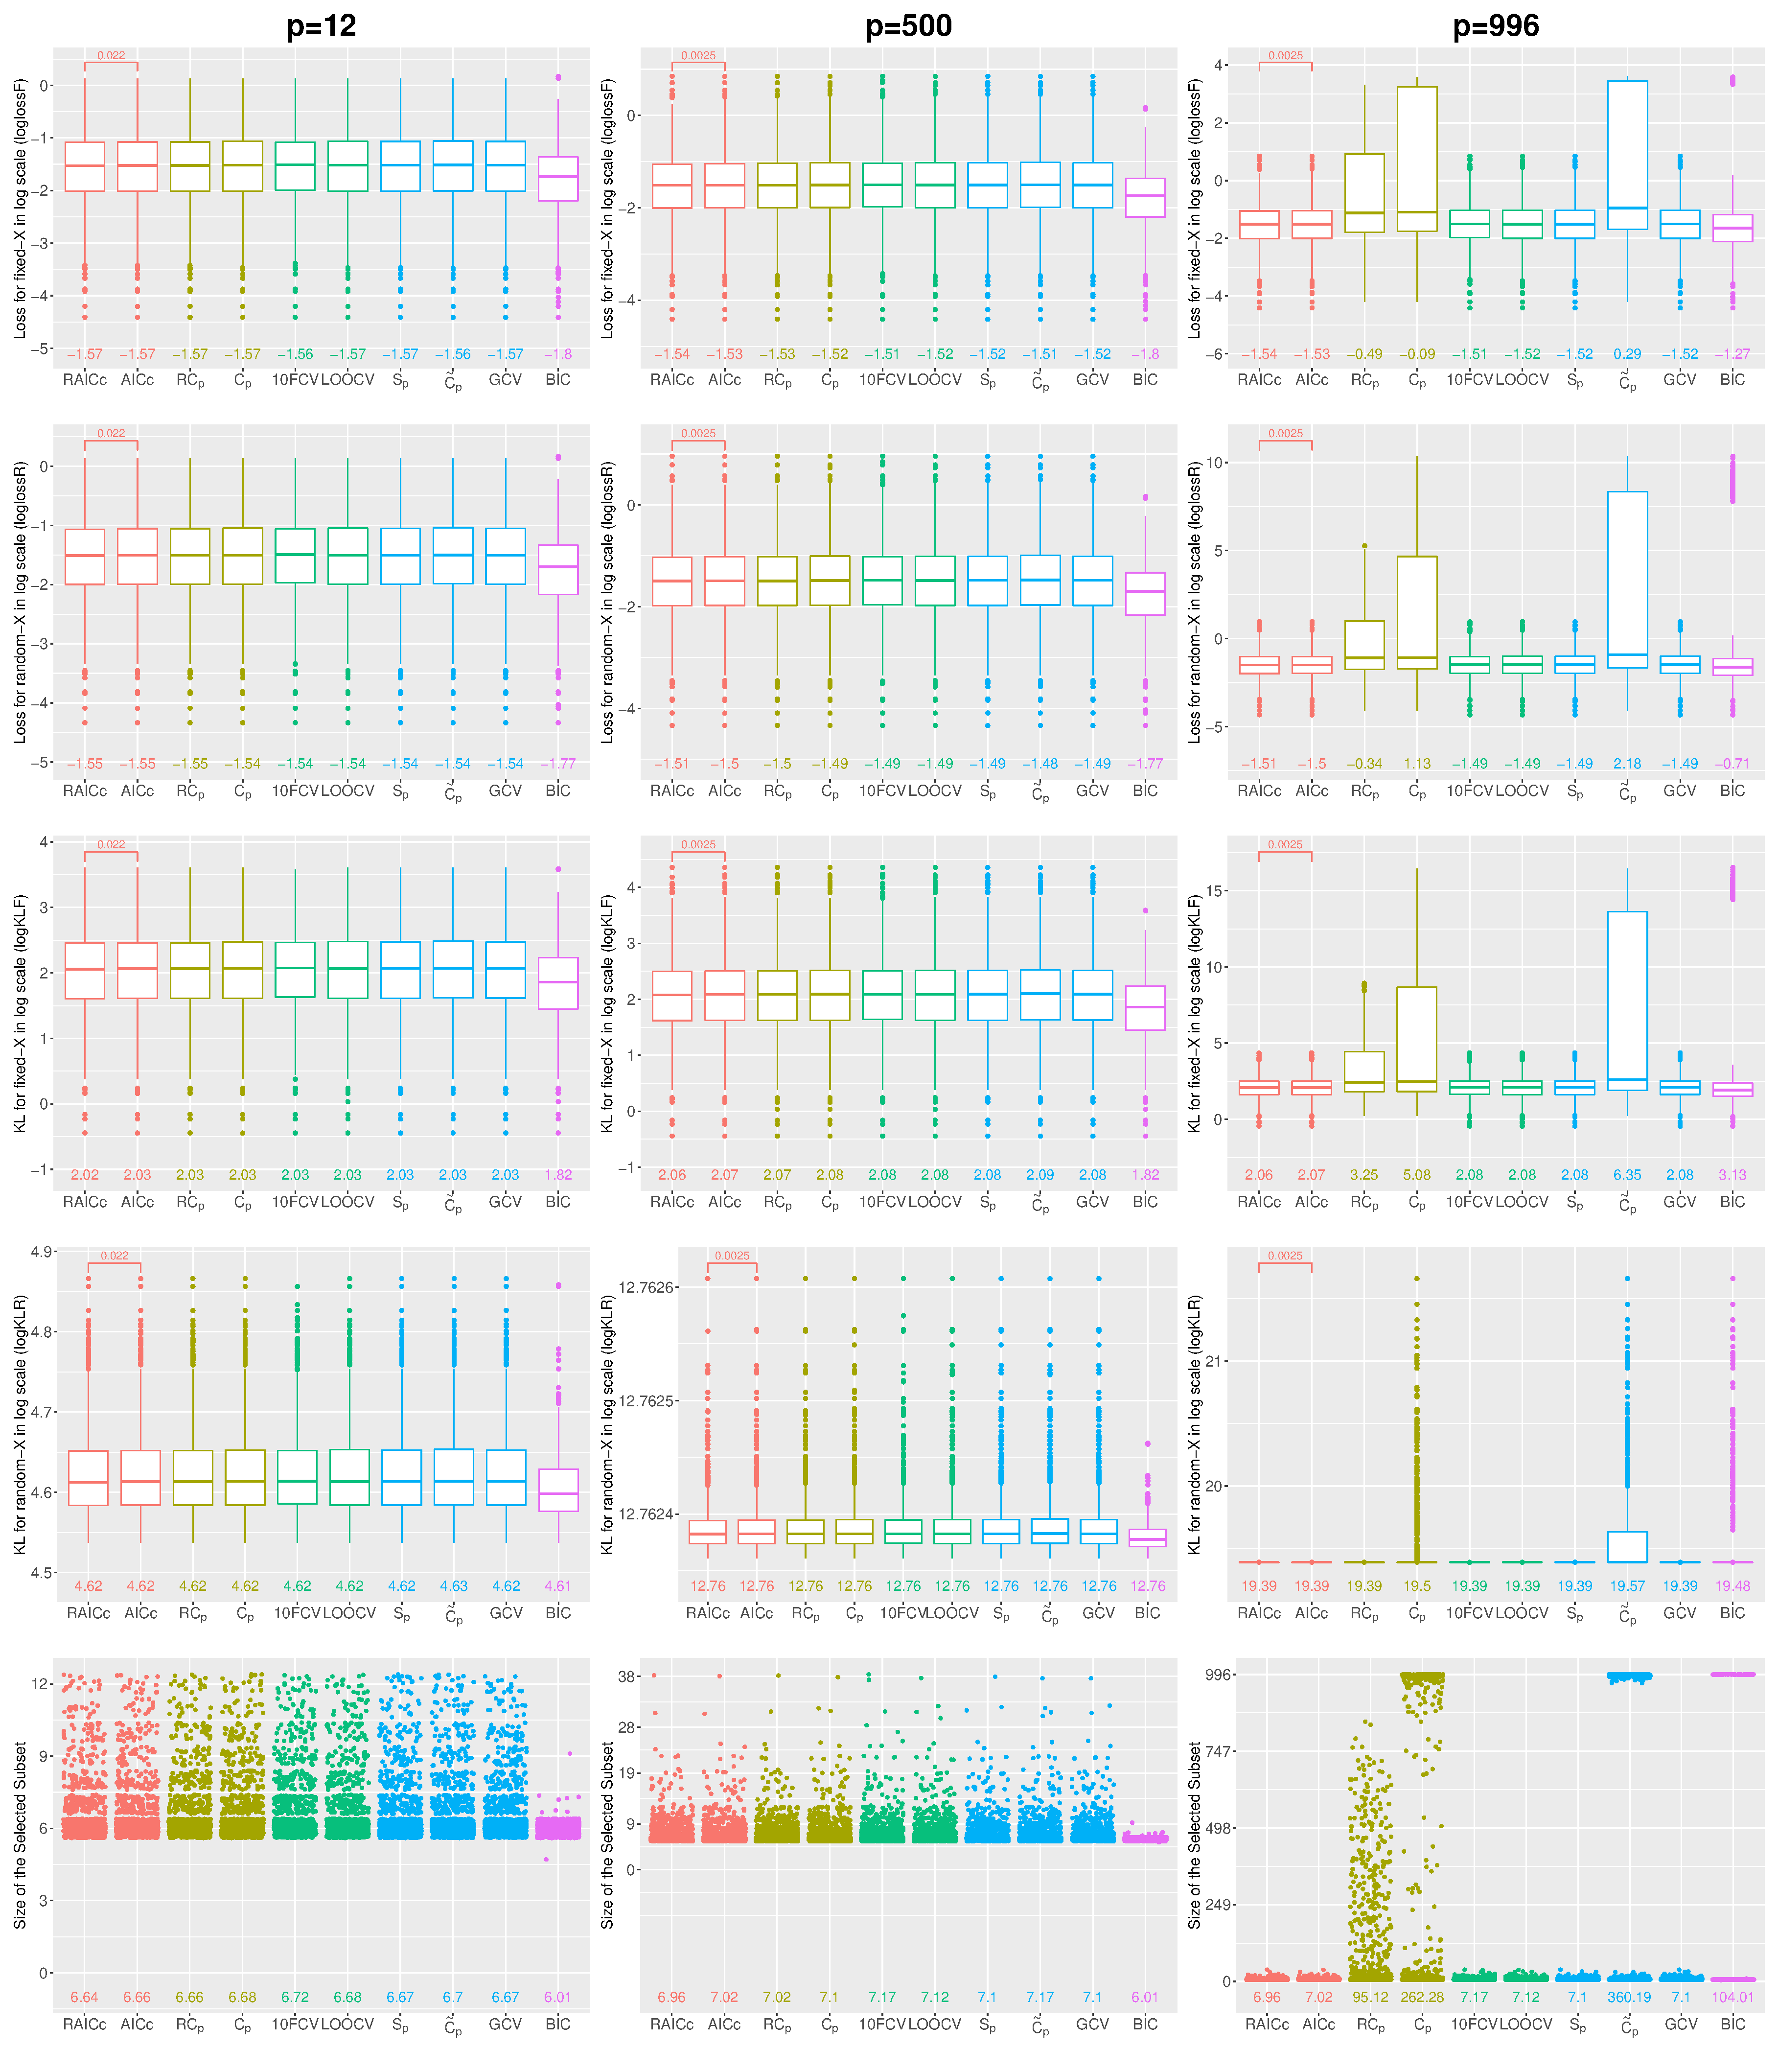
\includegraphics[width=\textwidth]{figures/supplement/fixedx/subset_selection/Sparse-Ex1_n1000_msnr_rho0.eps}
\caption{Variable selection, Fixed-X, Sparse-Ex1, $n=1000$, medium signal, and $\rho=0$.}
\end{figure}
\clearpage
\begin{figure}[!ht]
\centering
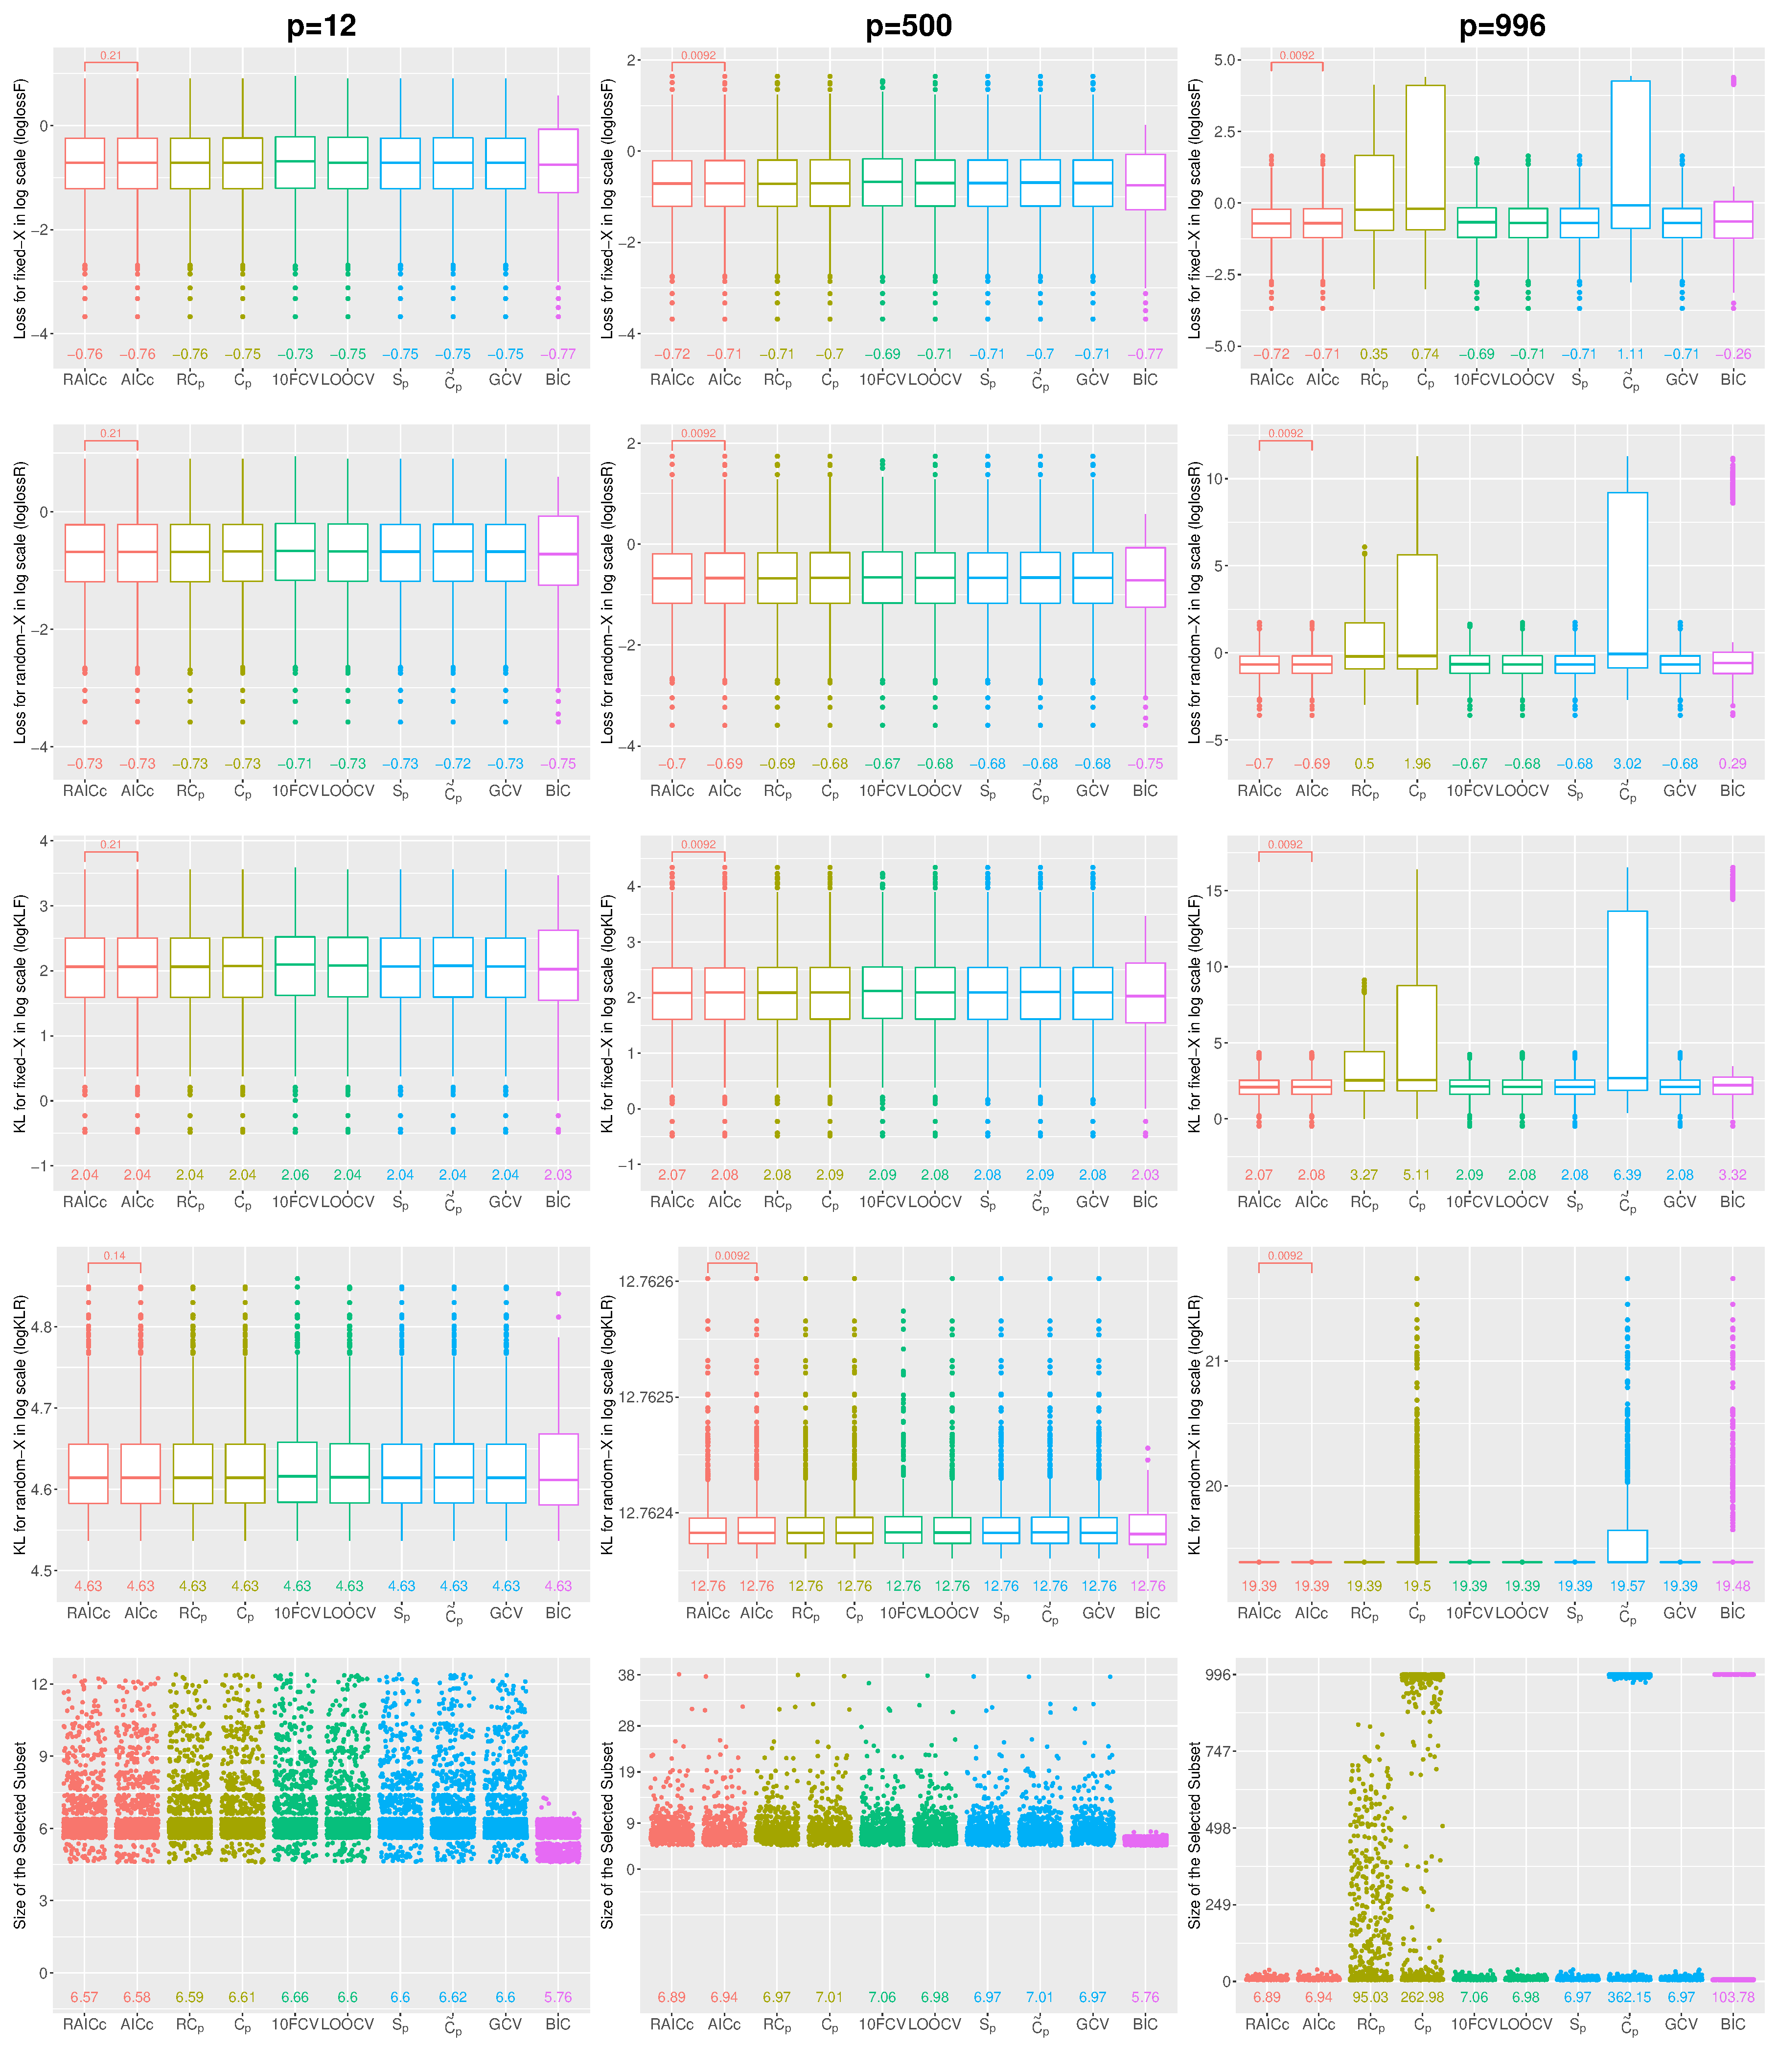
\includegraphics[width=\textwidth]{figures/supplement/fixedx/subset_selection/Sparse-Ex1_n1000_msnr_rho05.eps}
\caption{Variable selection, Fixed-X, Sparse-Ex1, $n=1000$, medium signal, and $\rho=0.5$.}
\end{figure}
\clearpage
\begin{figure}[!ht]
\centering
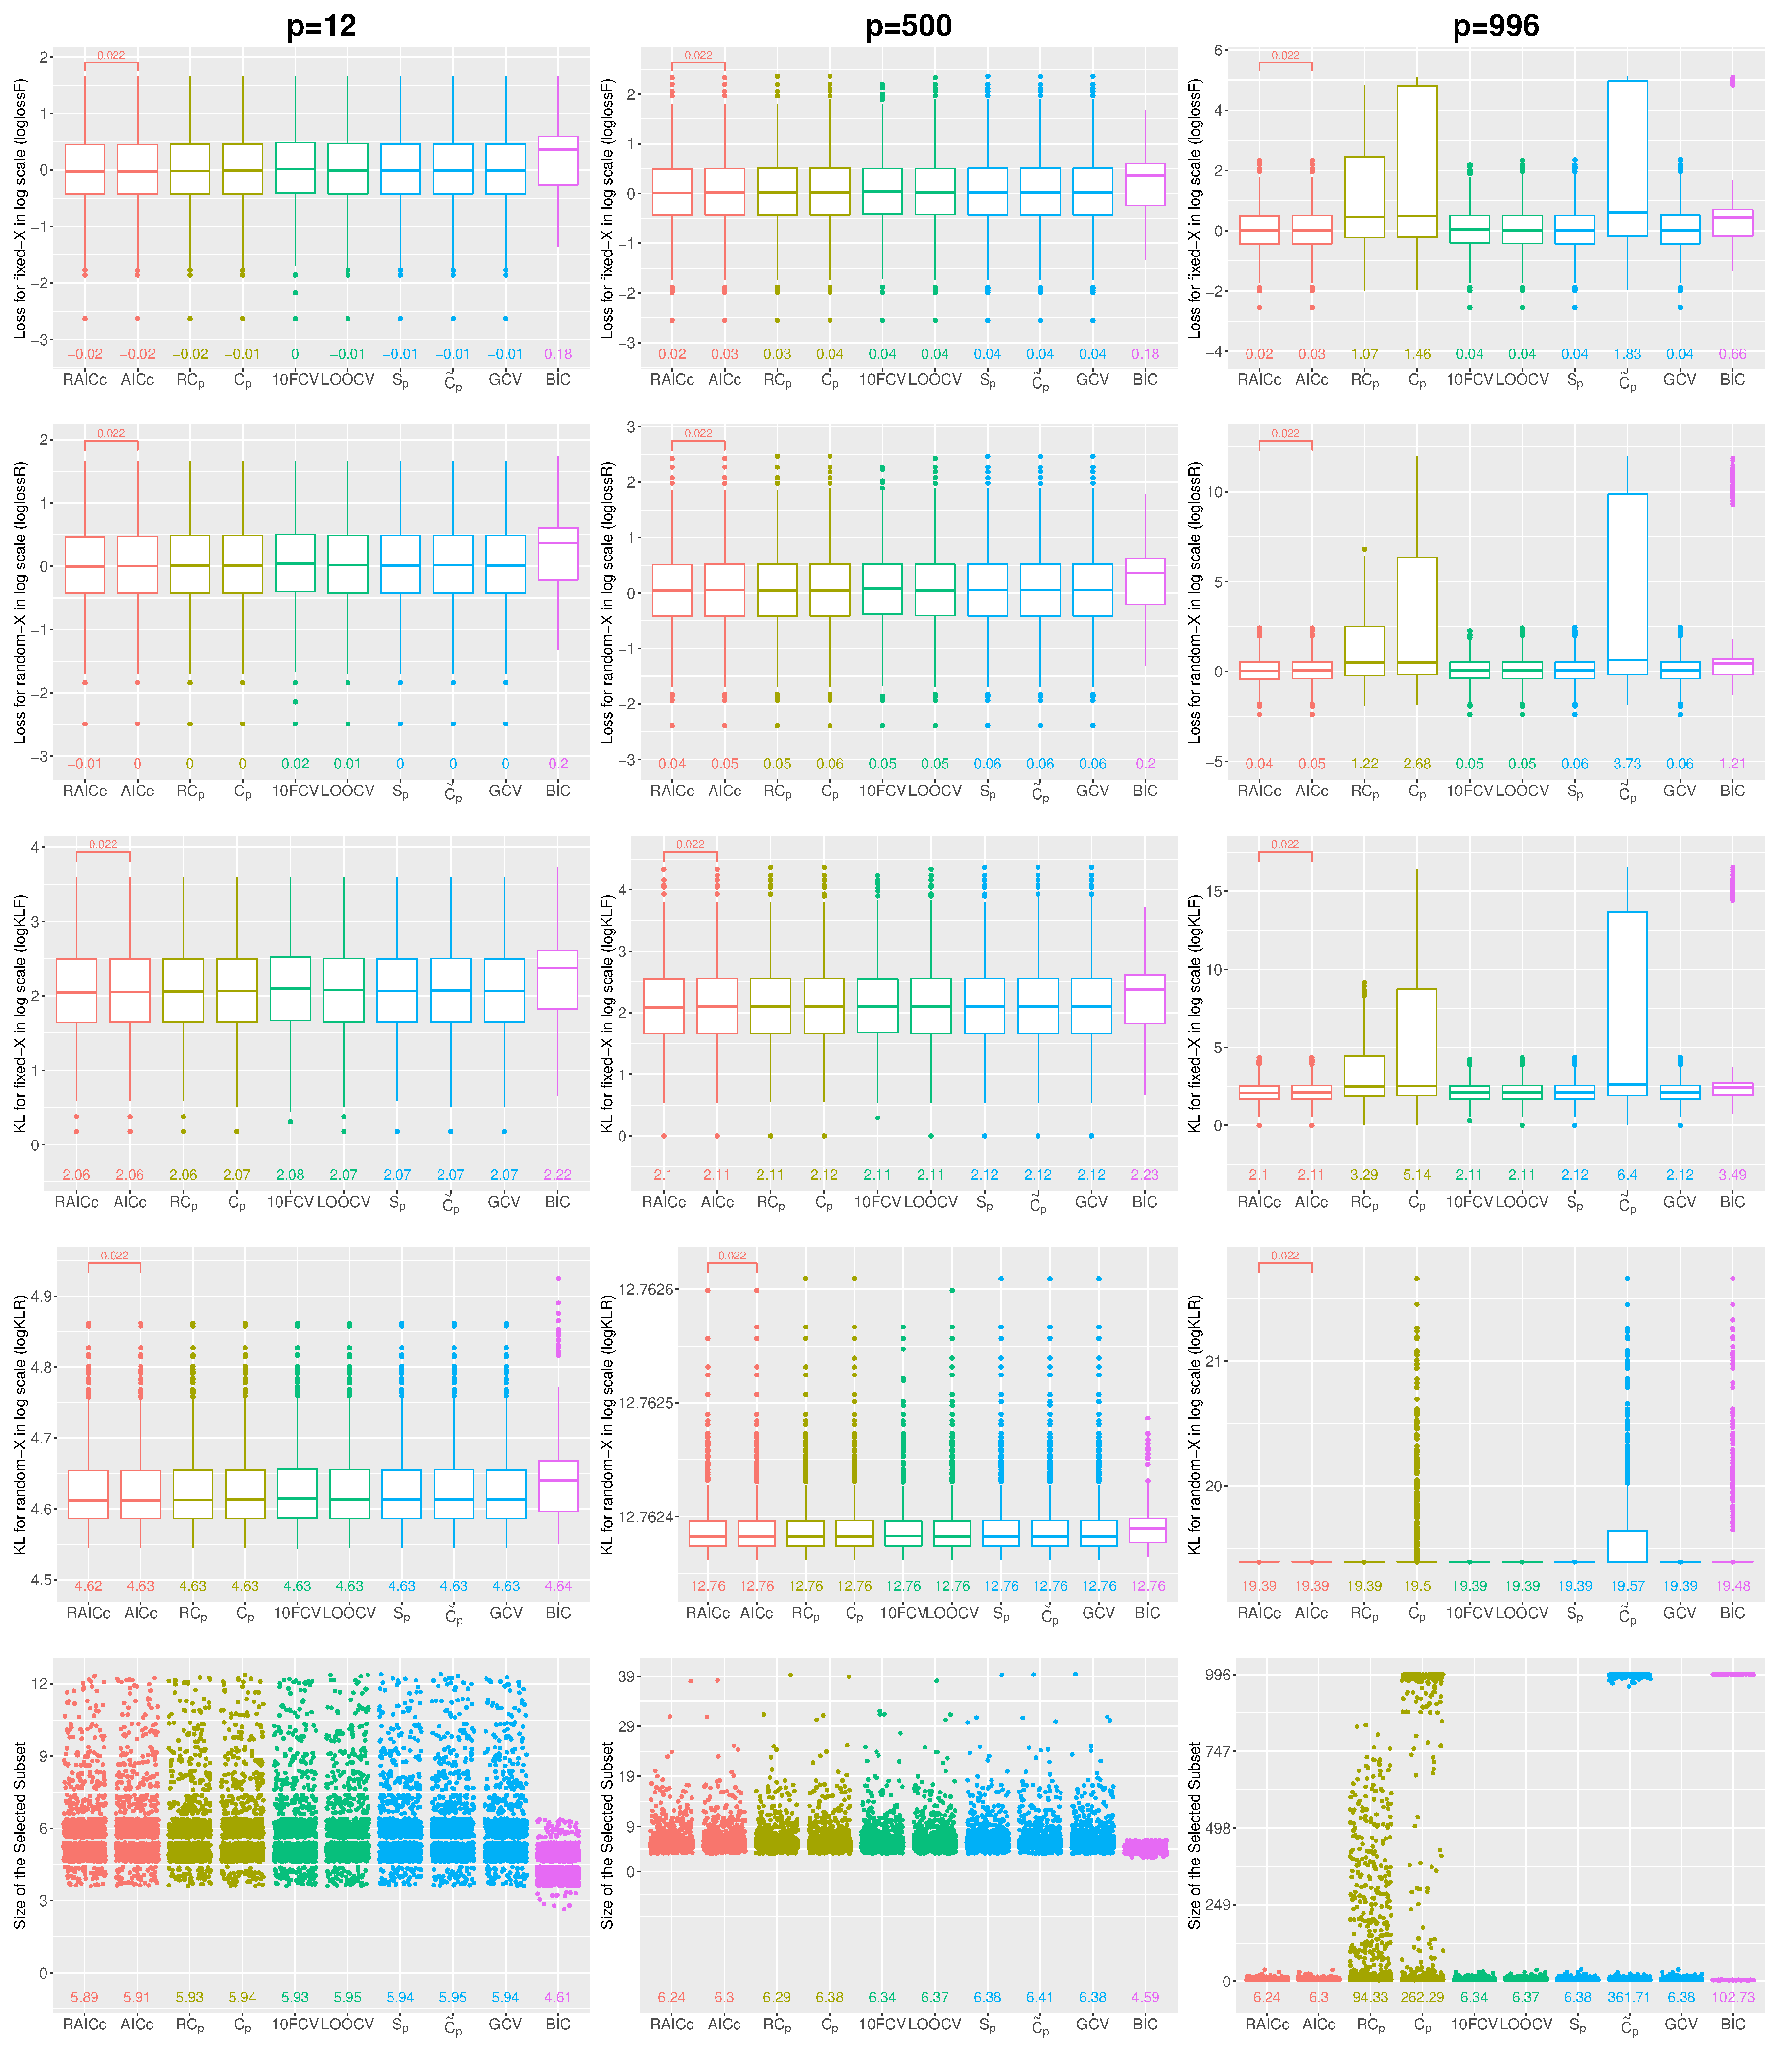
\includegraphics[width=\textwidth]{figures/supplement/fixedx/subset_selection/Sparse-Ex1_n1000_msnr_rho09.eps}
\caption{Variable selection, Fixed-X, Sparse-Ex1, $n=1000$, medium signal, and $\rho=0.9$.}
\end{figure}
\clearpage
\begin{figure}[!ht]
\centering
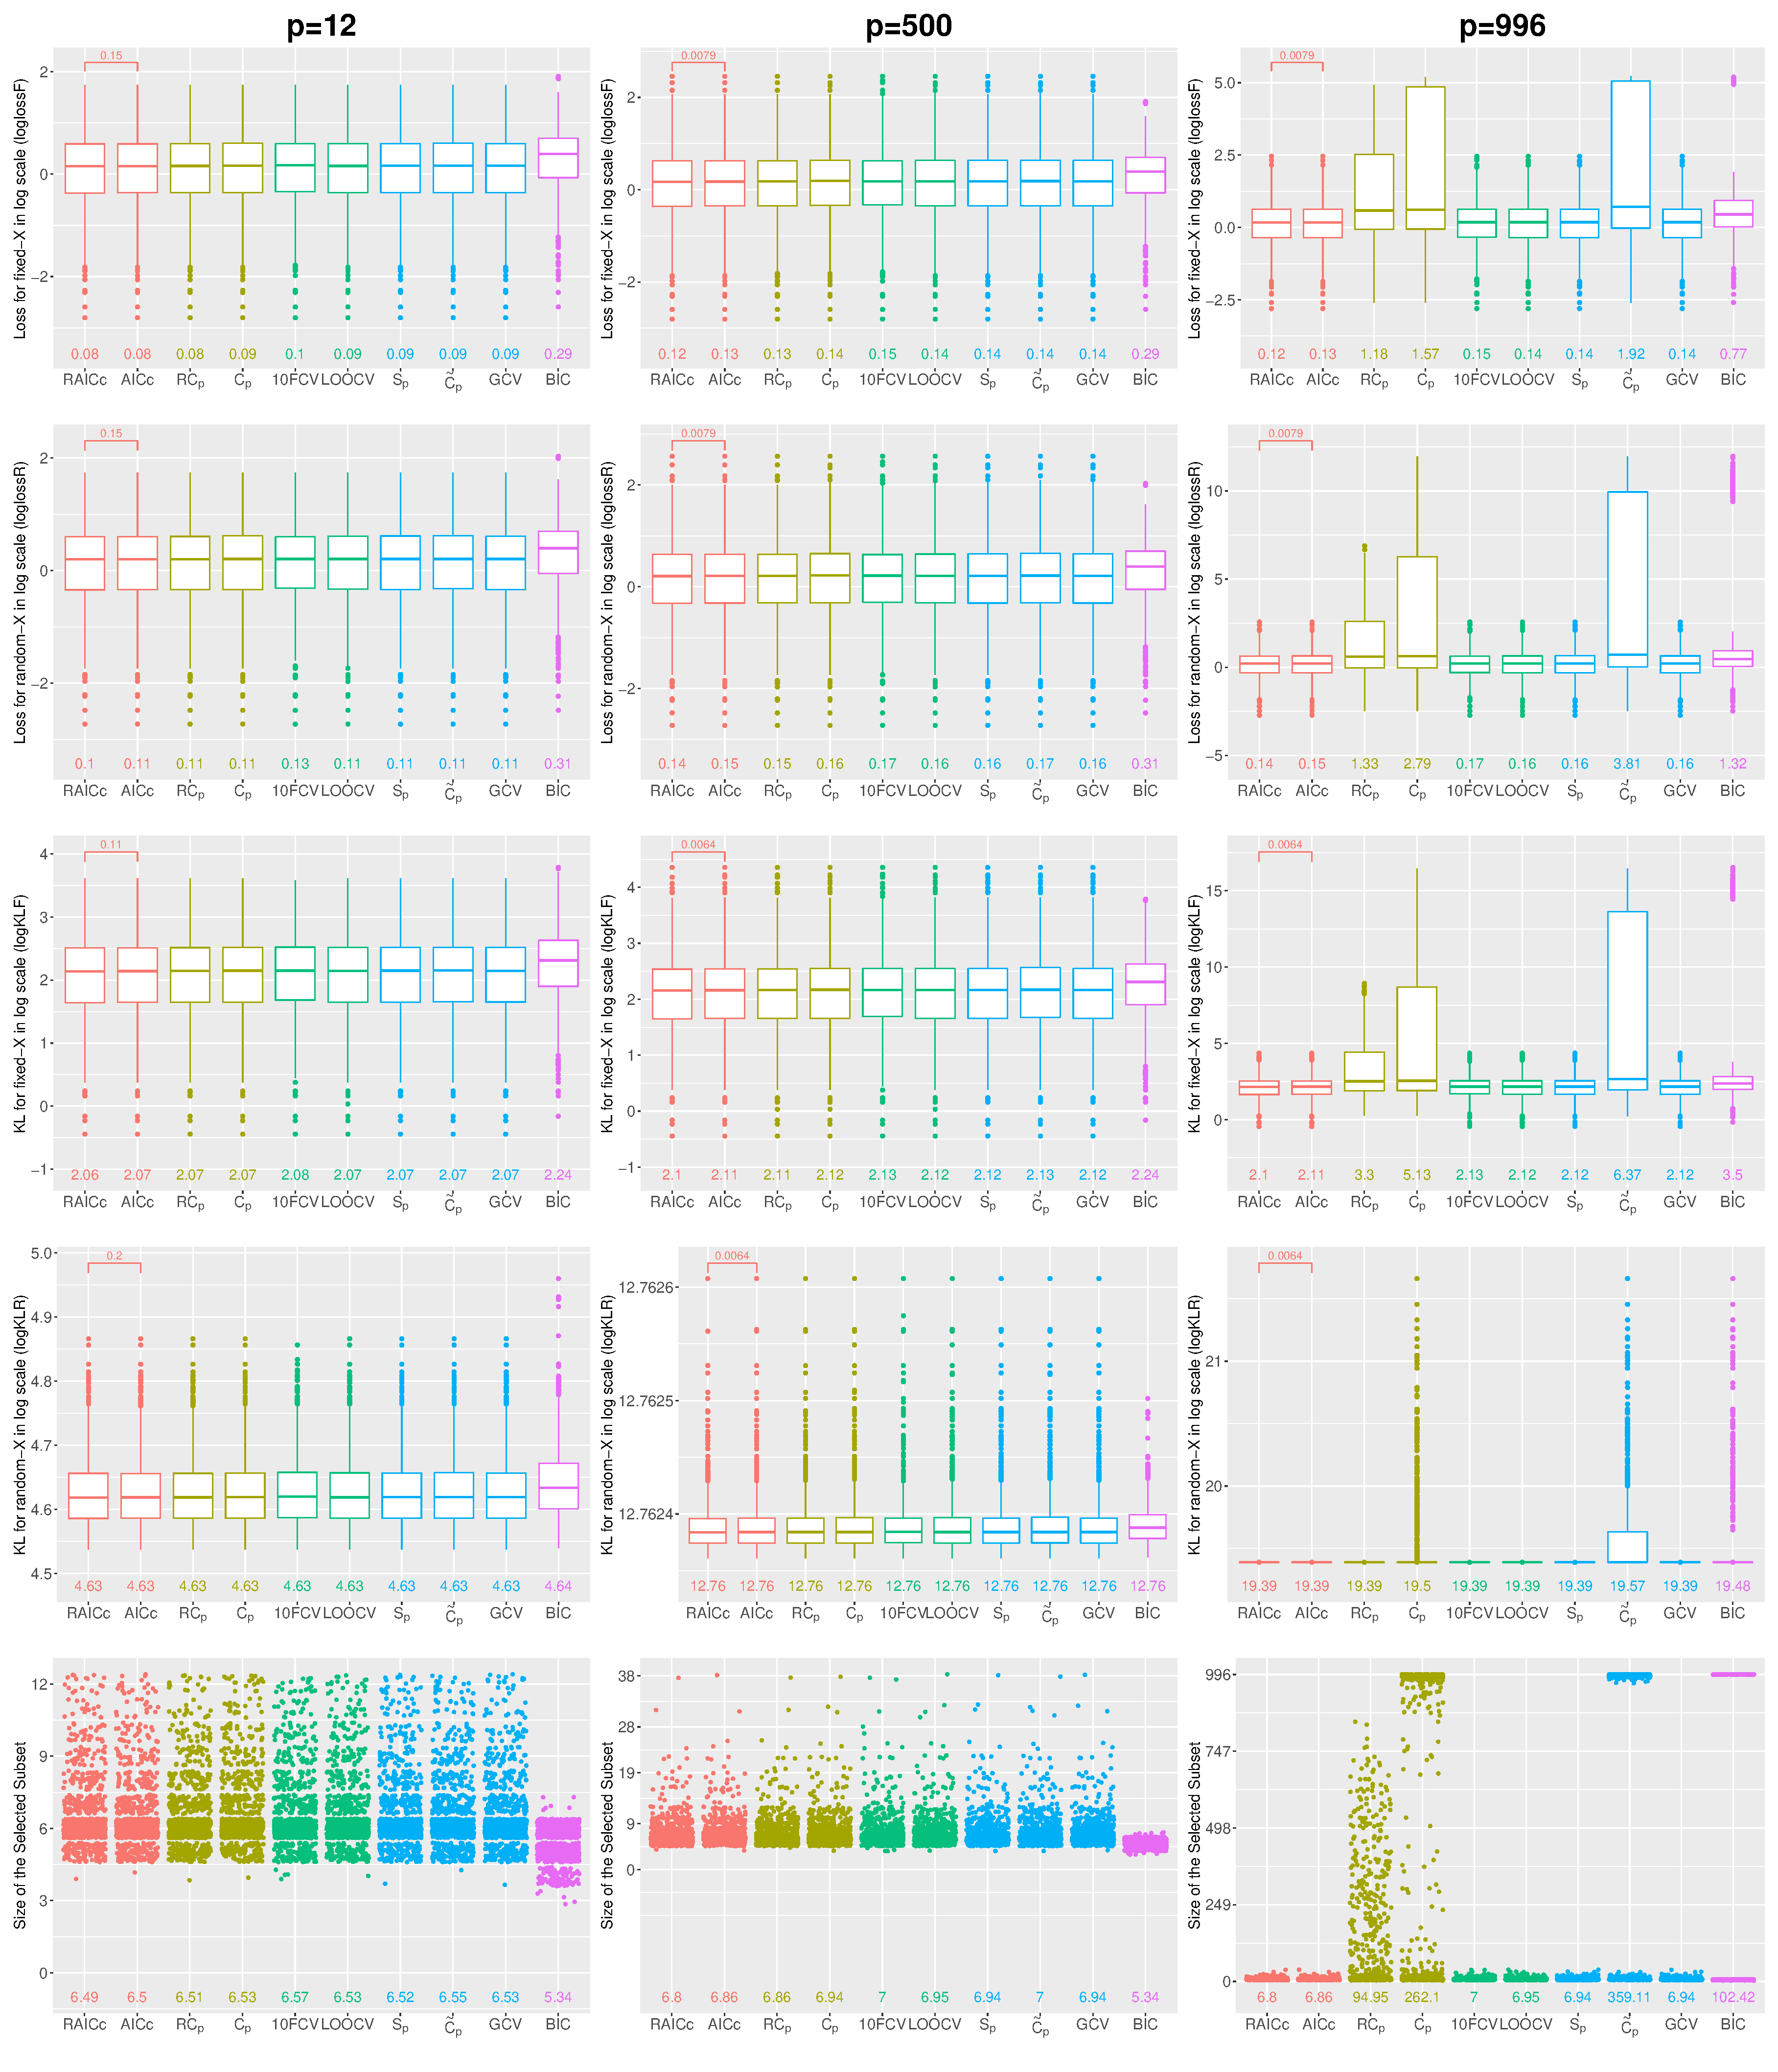
\includegraphics[width=\textwidth]{figures/supplement/fixedx/subset_selection/Sparse-Ex1_n1000_lsnr_rho0.eps}
\caption{Variable selection, Fixed-X, Sparse-Ex1, $n=1000$, low signal, and $\rho=0$.}
\end{figure}
\clearpage
\begin{figure}[!ht]
\centering
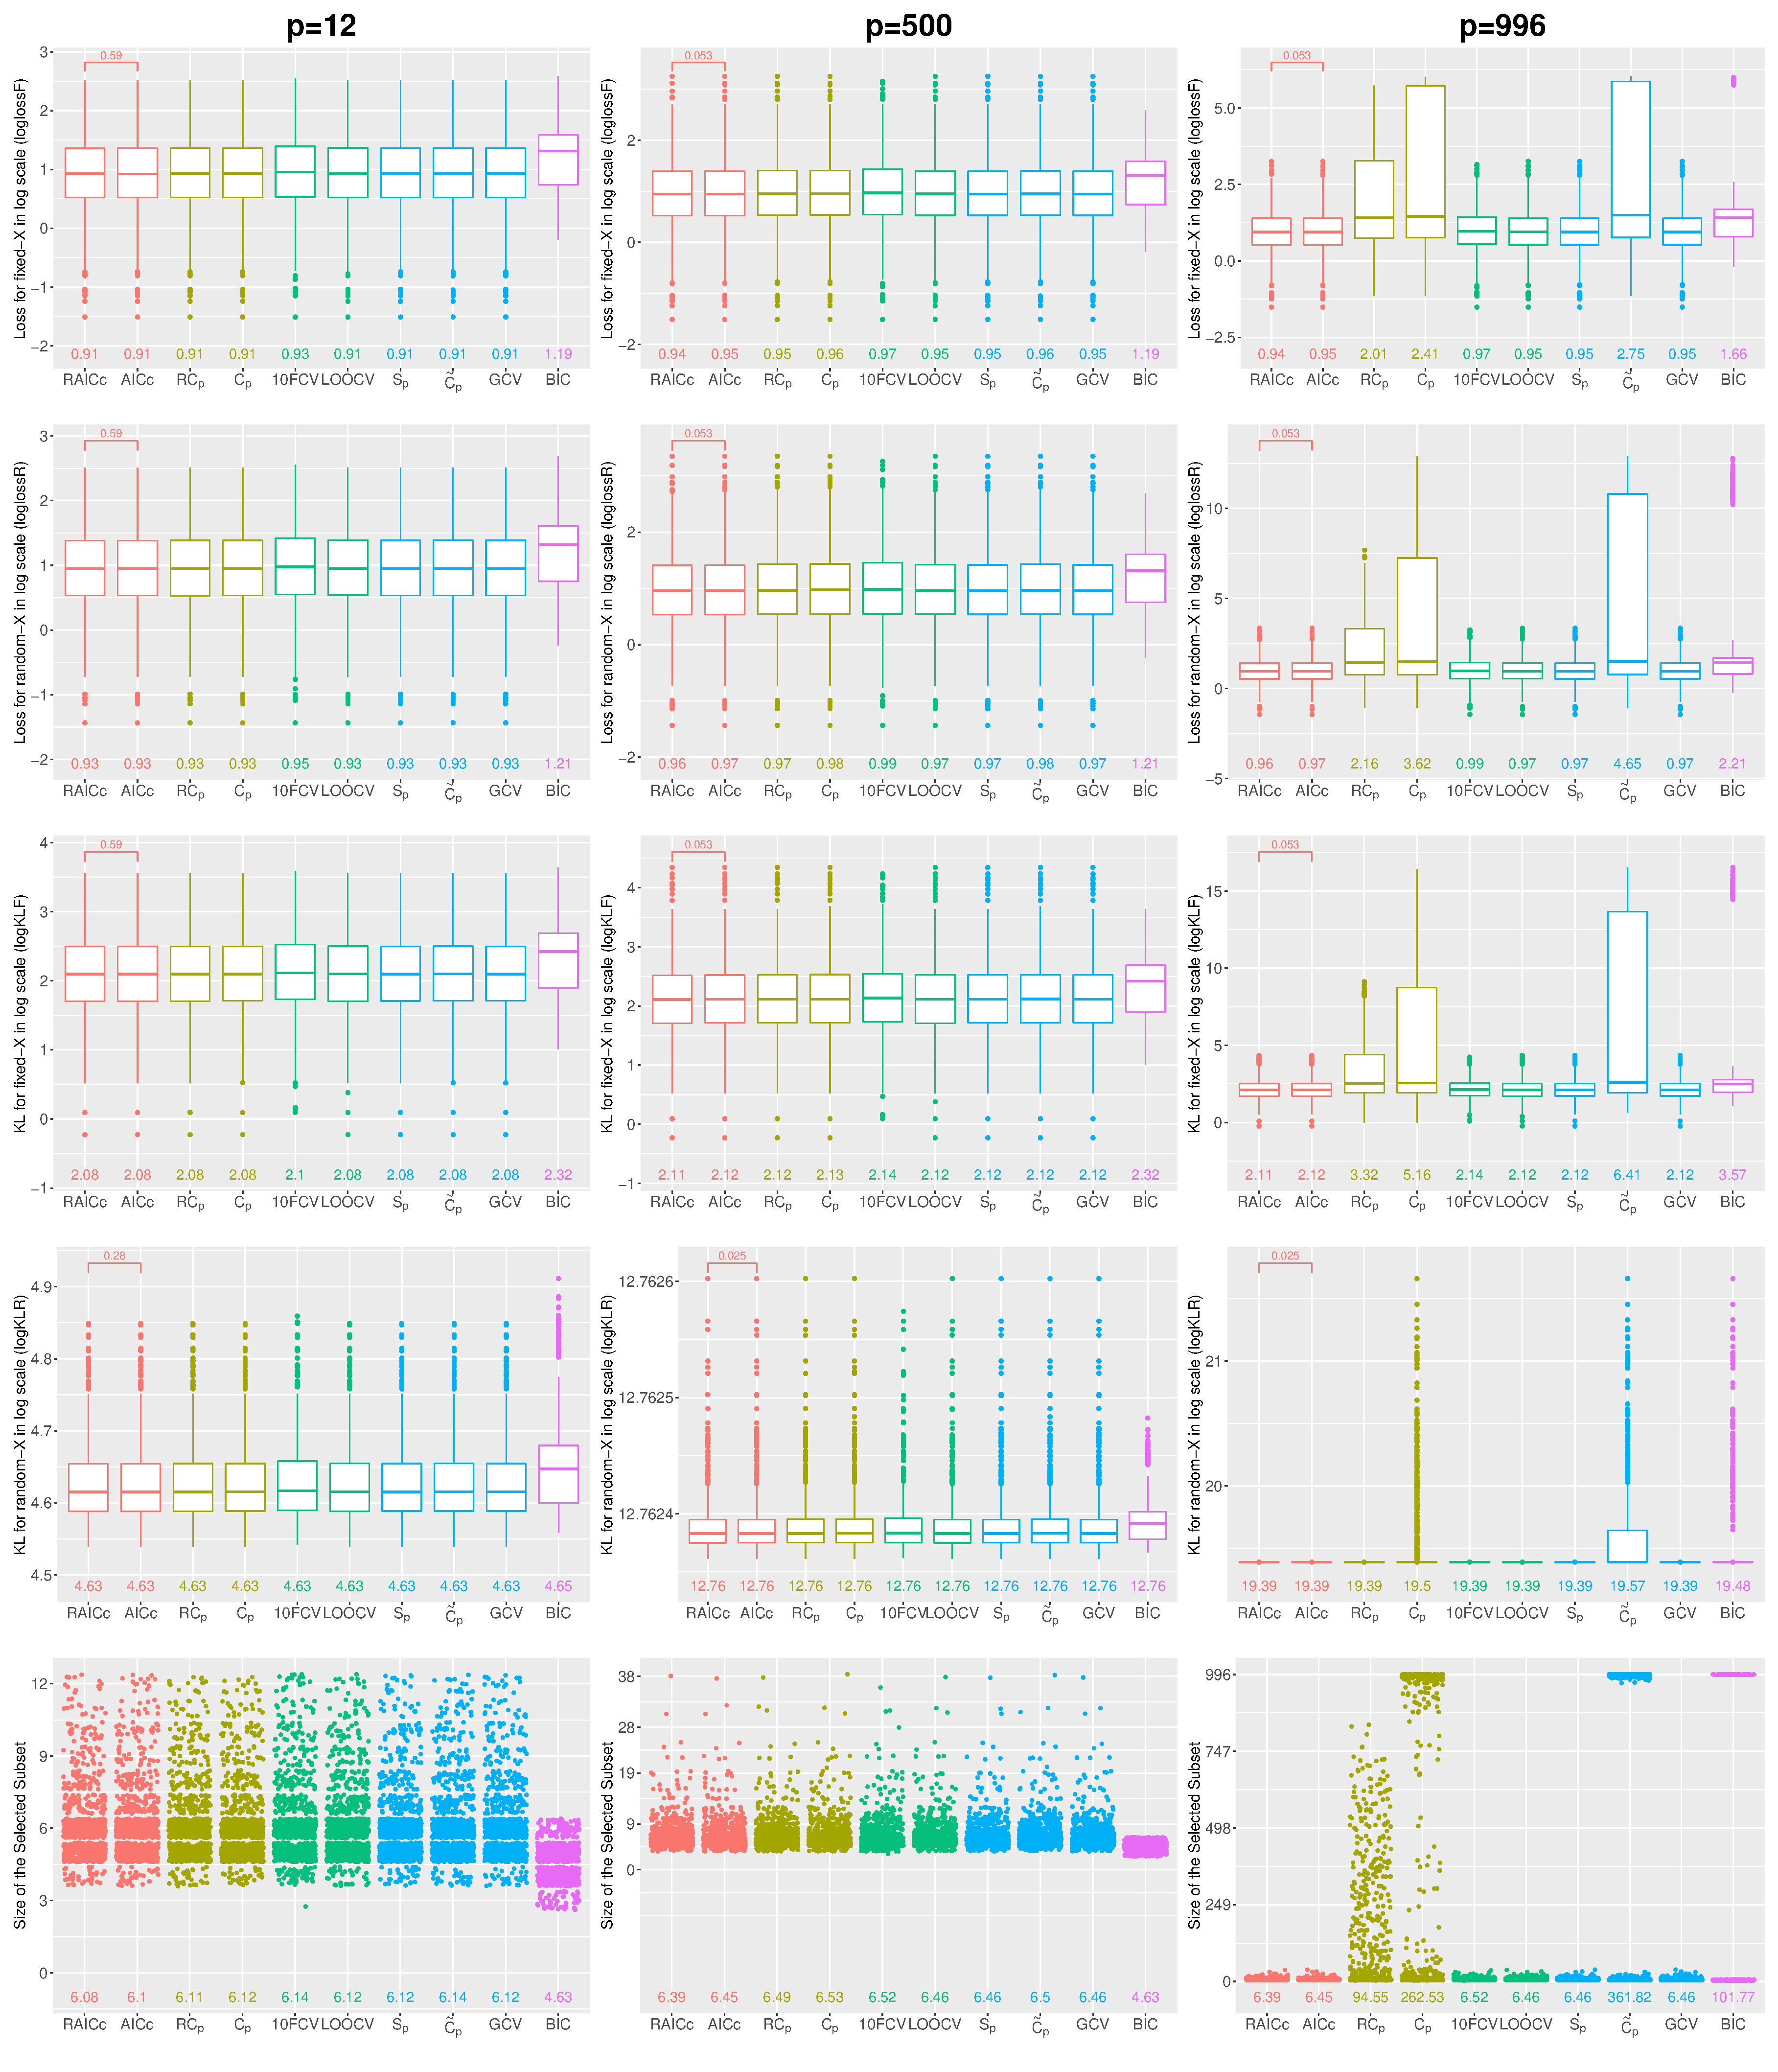
\includegraphics[width=\textwidth]{figures/supplement/fixedx/subset_selection/Sparse-Ex1_n1000_lsnr_rho05.eps}
\caption{Variable selection, Fixed-X, Sparse-Ex1, $n=1000$, low signal, and $\rho=0.5$.}
\end{figure}
\clearpage
\begin{figure}[!ht]
\centering
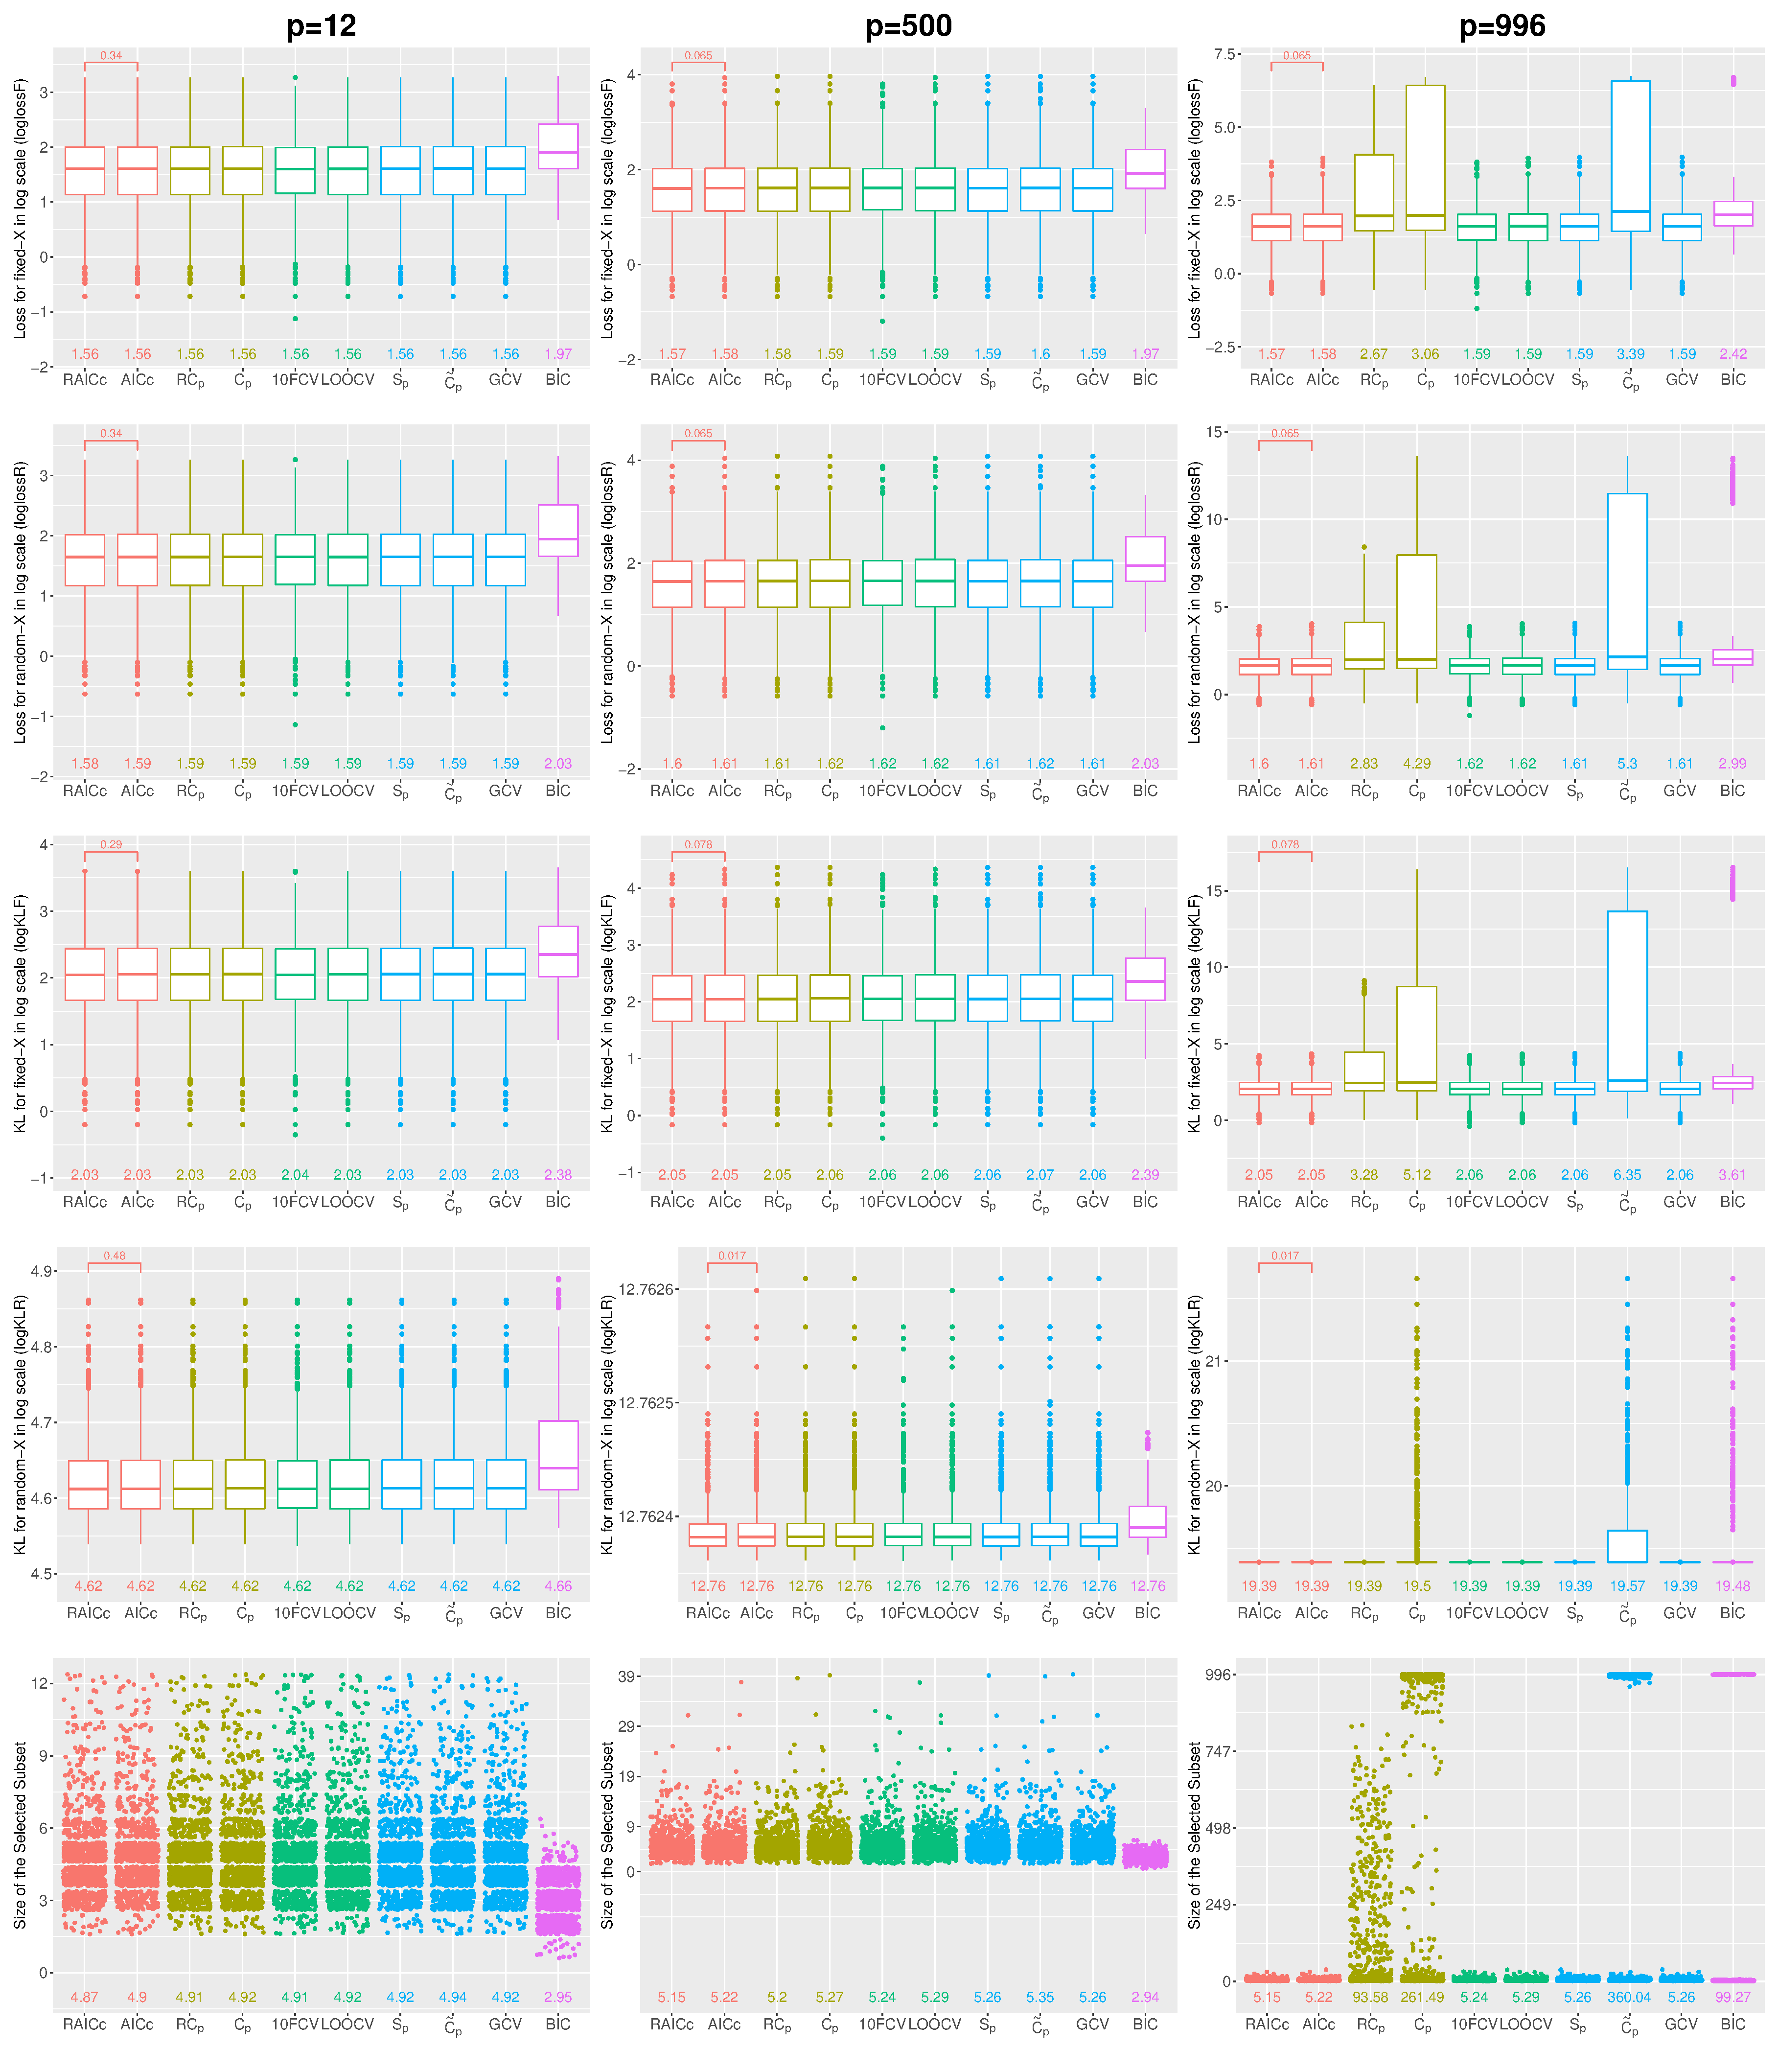
\includegraphics[width=\textwidth]{figures/supplement/fixedx/subset_selection/Sparse-Ex1_n1000_lsnr_rho09.eps}
\caption{Variable selection, Fixed-X, Sparse-Ex1, $n=1000$, low signal, and $\rho=0.9$.}
\end{figure}
\clearpage
\begin{figure}[!ht]
\centering
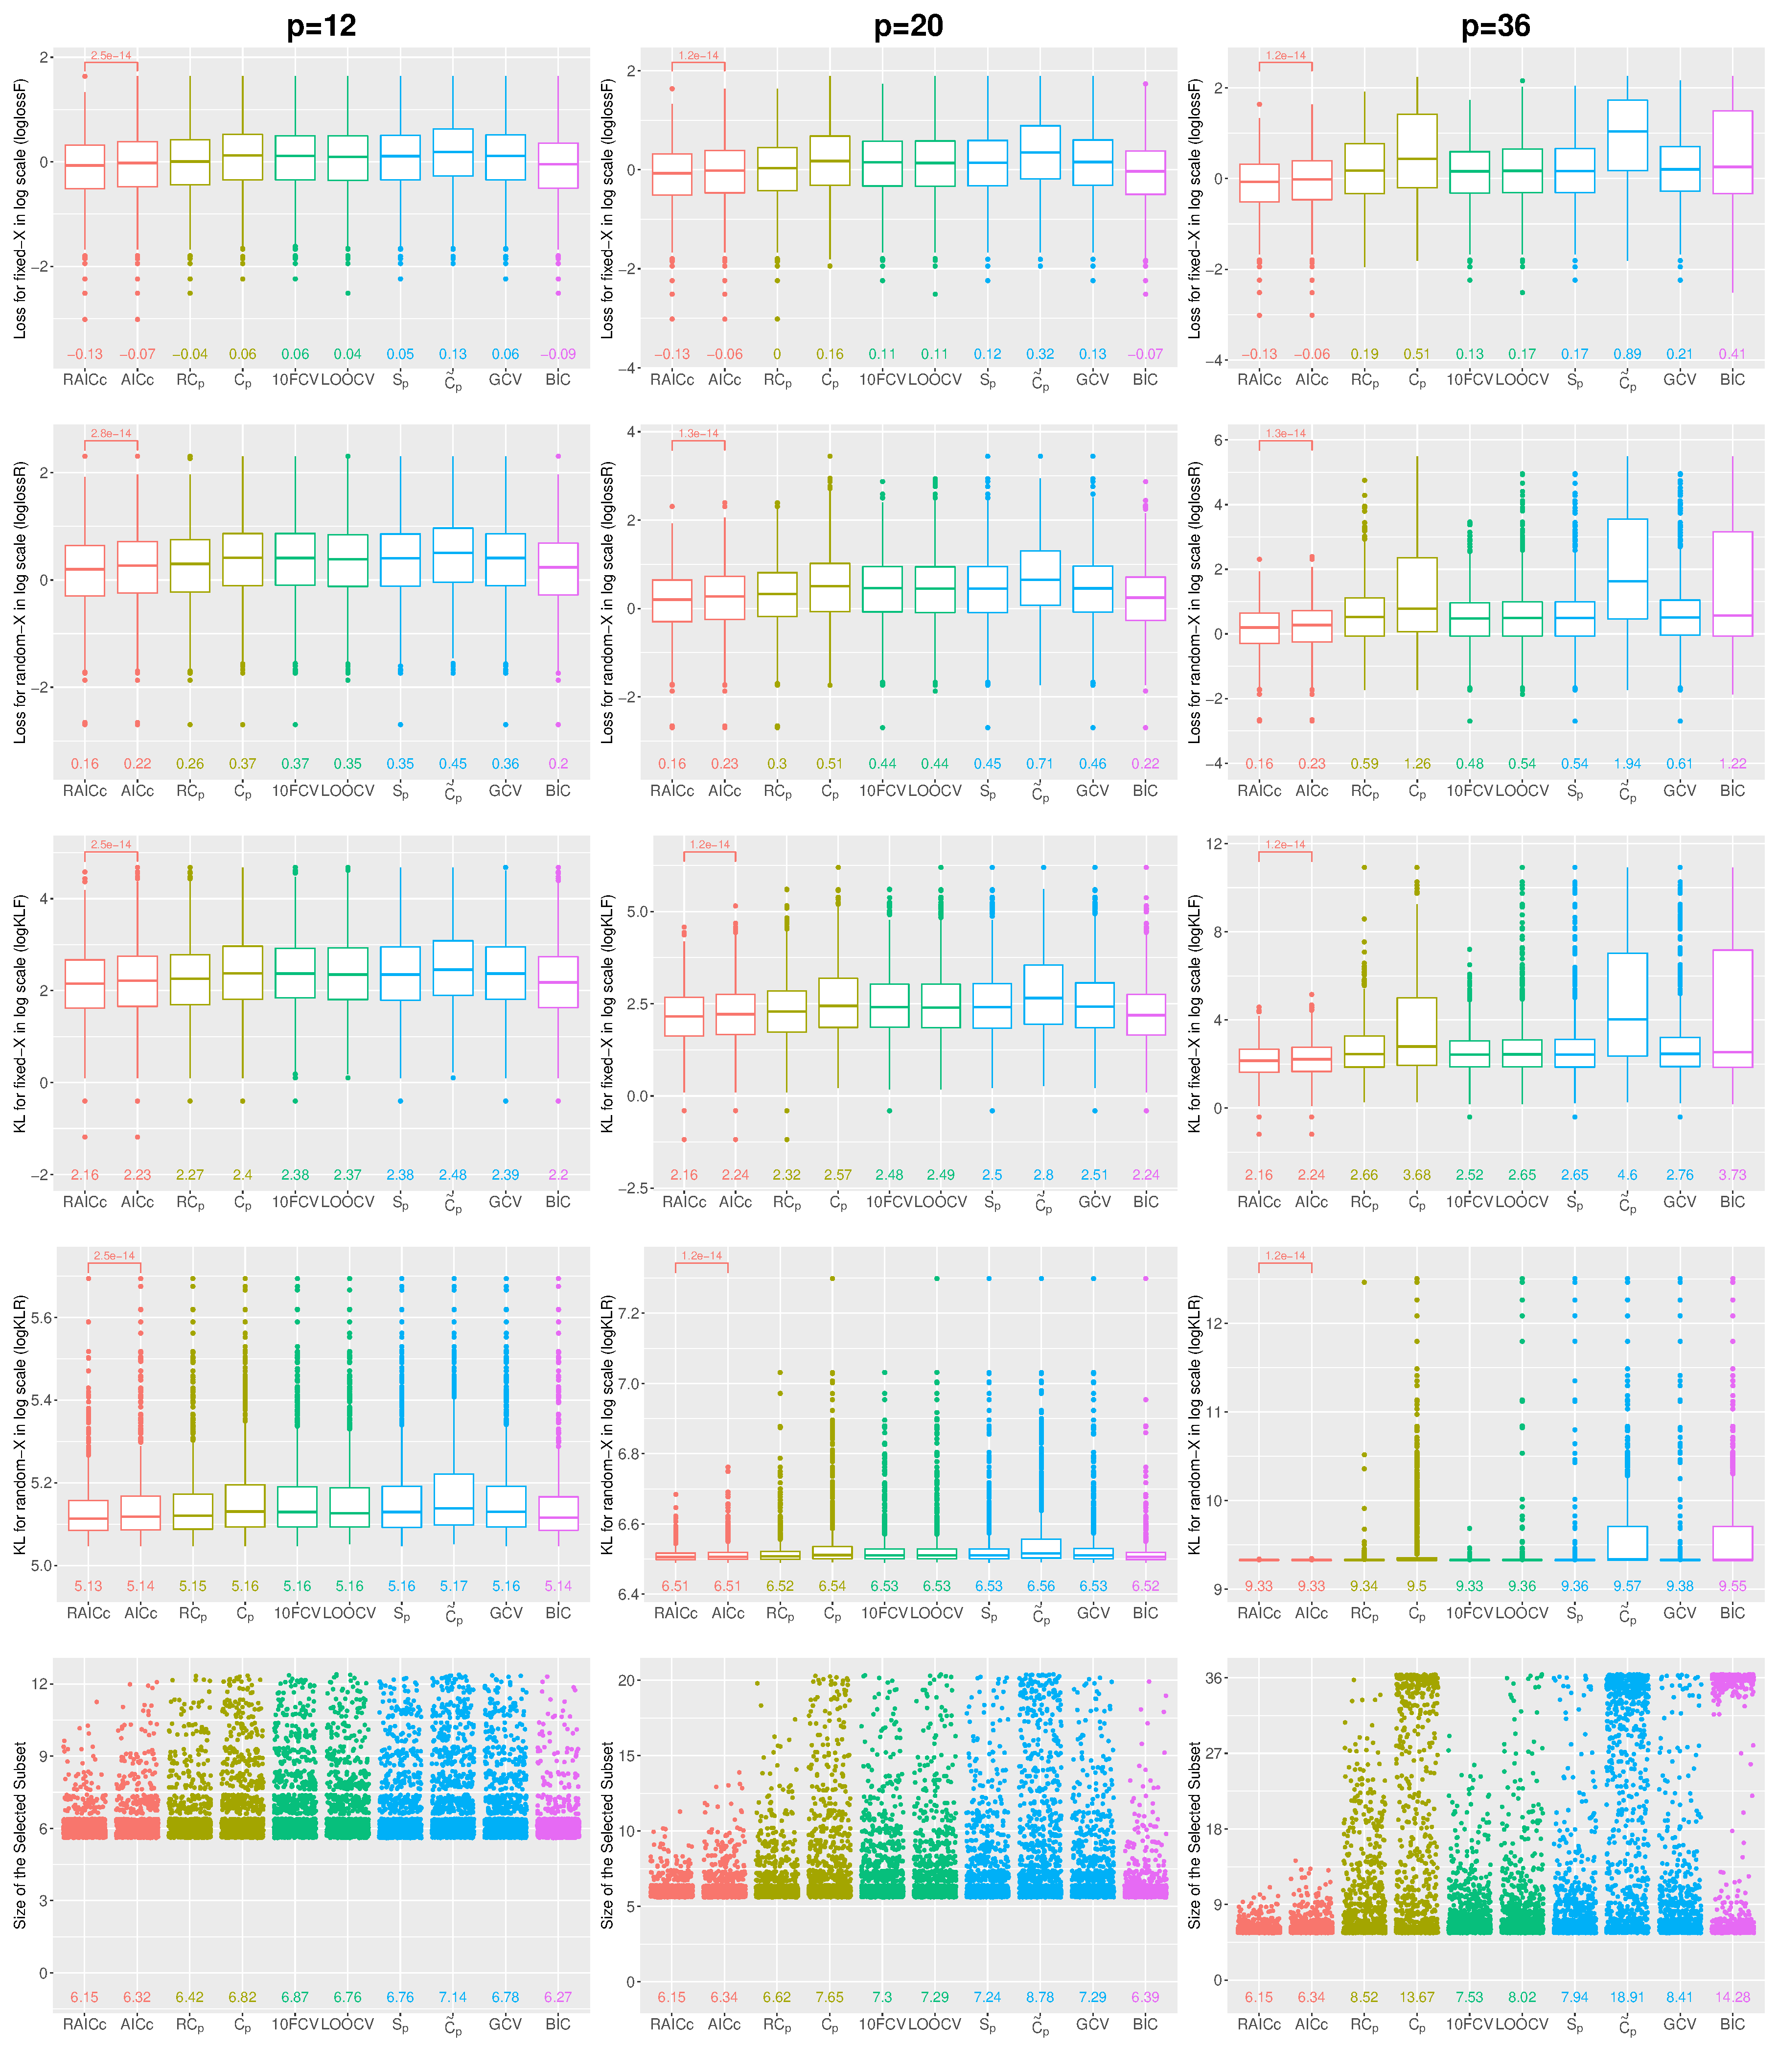
\includegraphics[width=\textwidth]{figures/supplement/fixedx/subset_selection/Sparse-Ex2_n40_hsnr_rho0.eps}
\caption{Variable selection, Fixed-X, Sparse-Ex2, $n=40$, high signal, and $\rho=0$.}
\end{figure}
\clearpage
\begin{figure}[!ht]
\centering
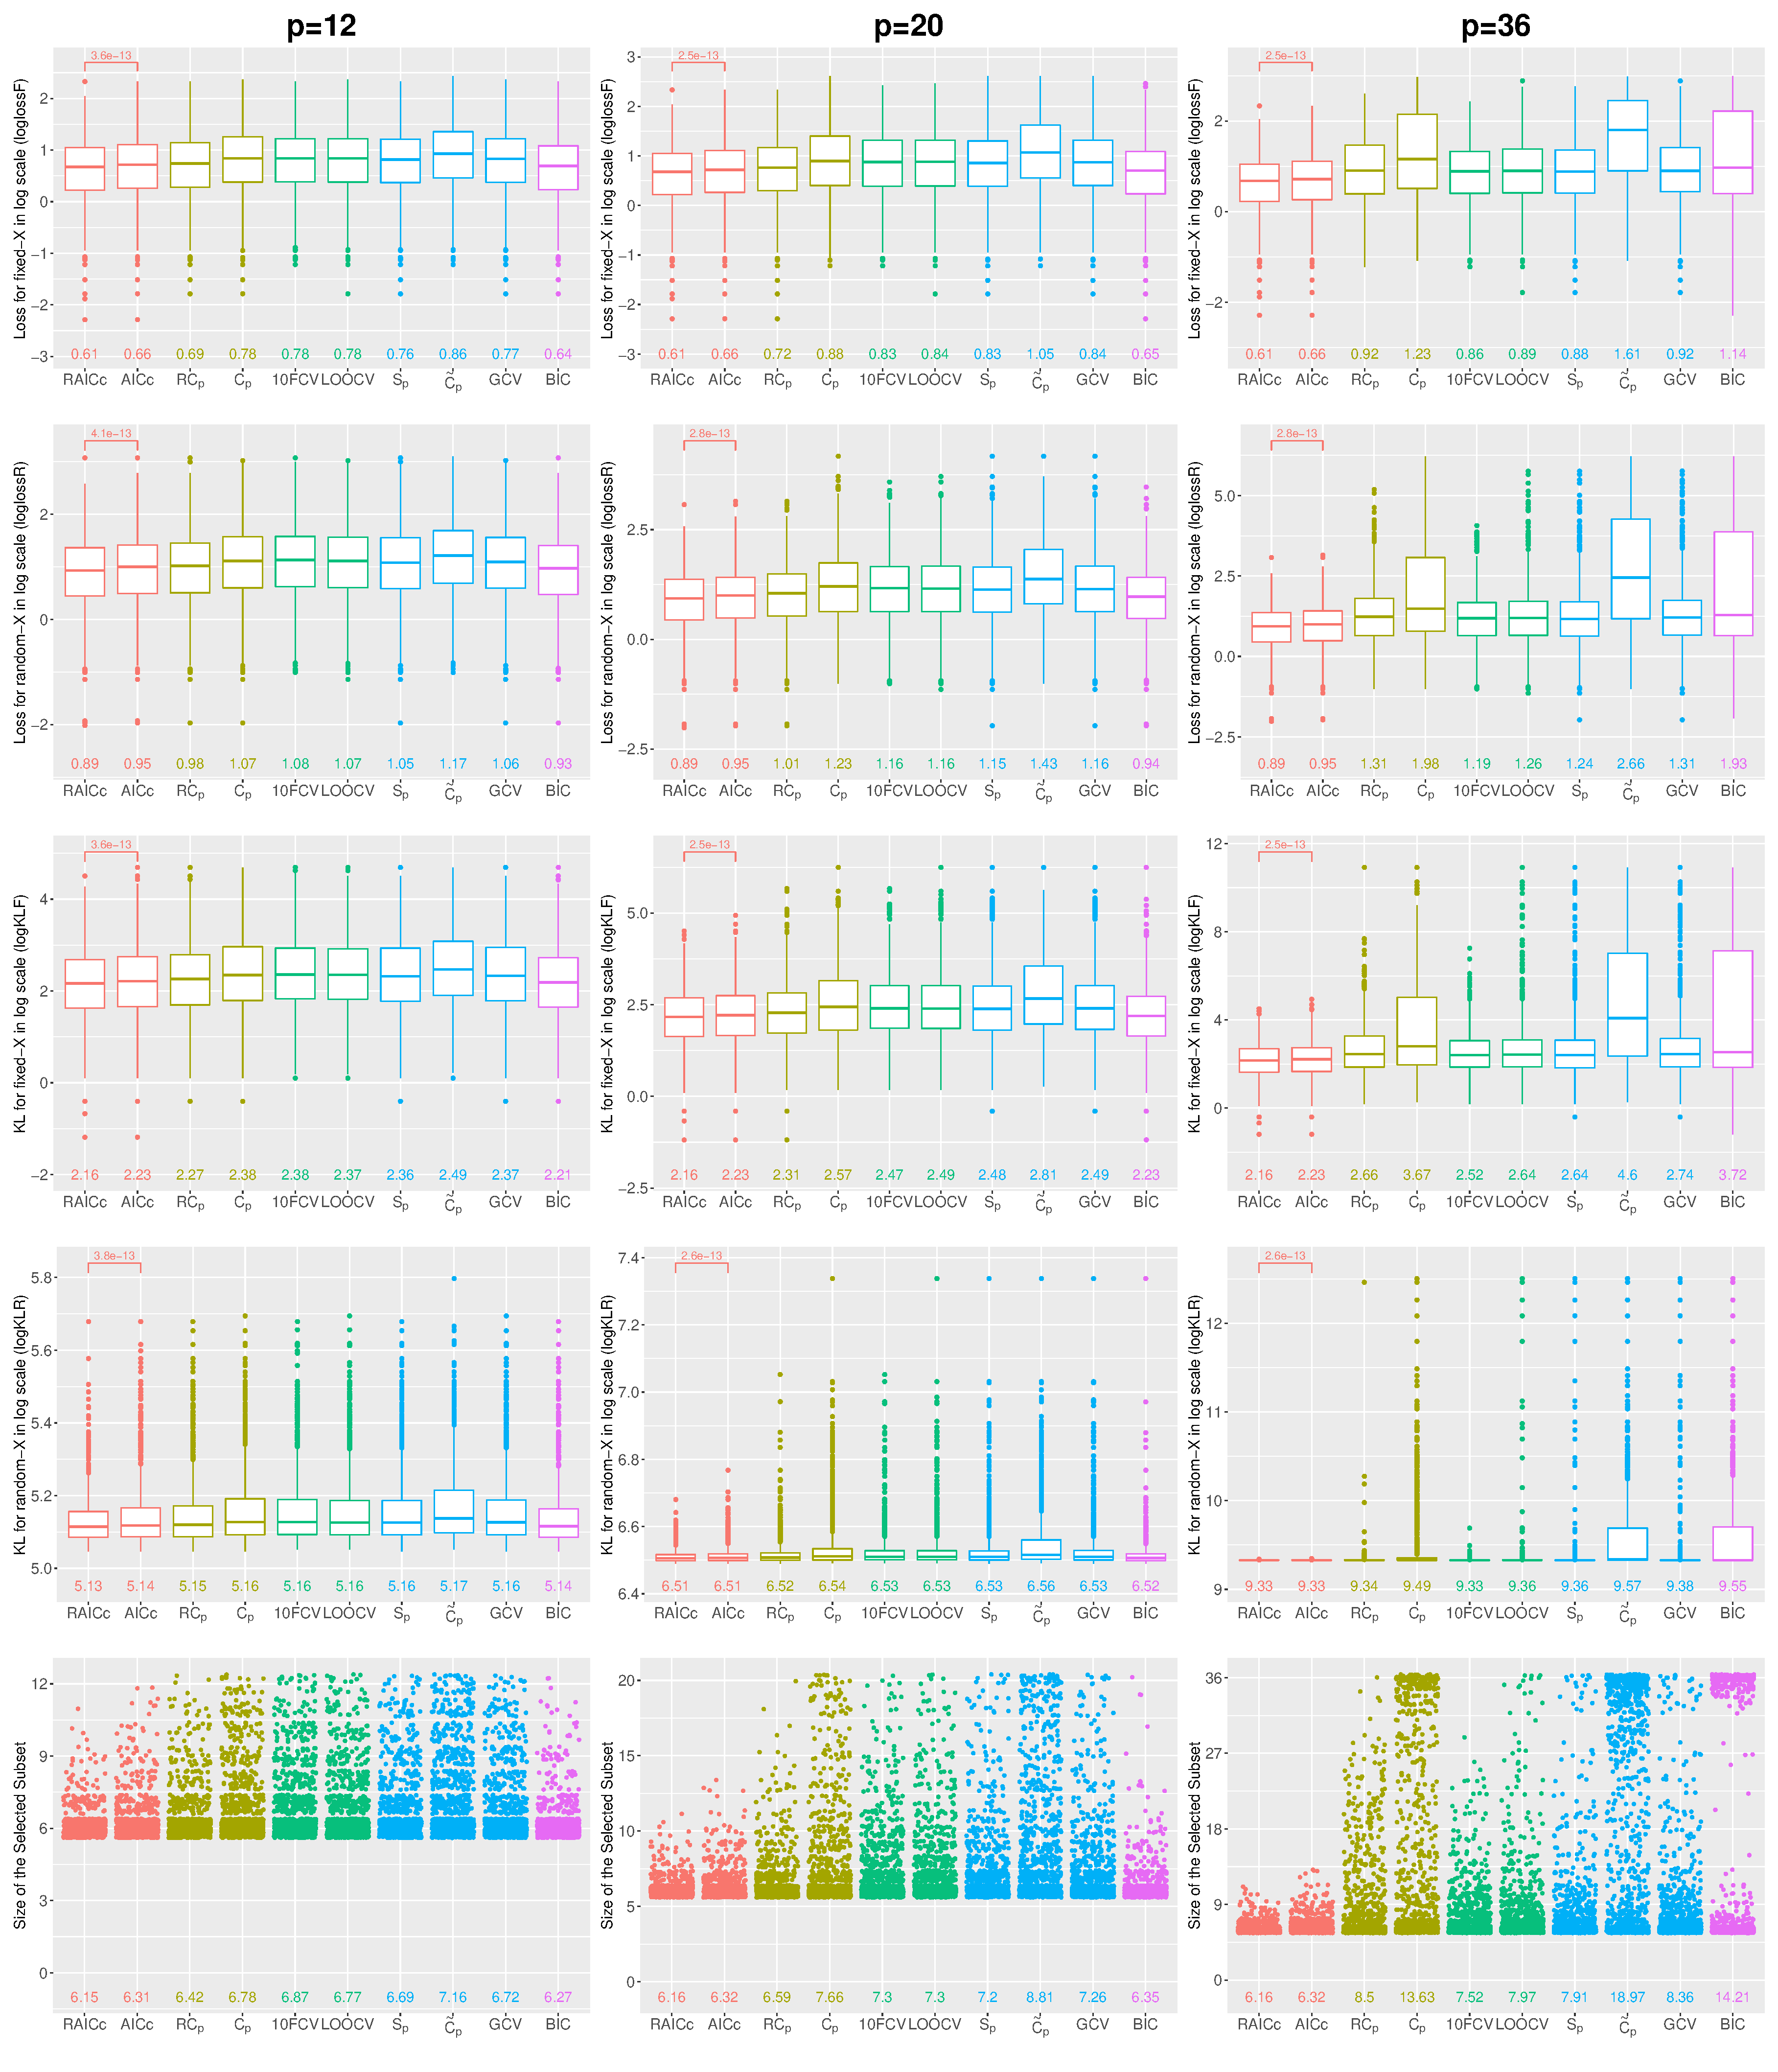
\includegraphics[width=\textwidth]{figures/supplement/fixedx/subset_selection/Sparse-Ex2_n40_hsnr_rho05.eps}
\caption{Variable selection, Fixed-X, Sparse-Ex2, $n=40$, high signal, and $\rho=0.5$.}
\end{figure}
\clearpage
\begin{figure}[!ht]
\centering
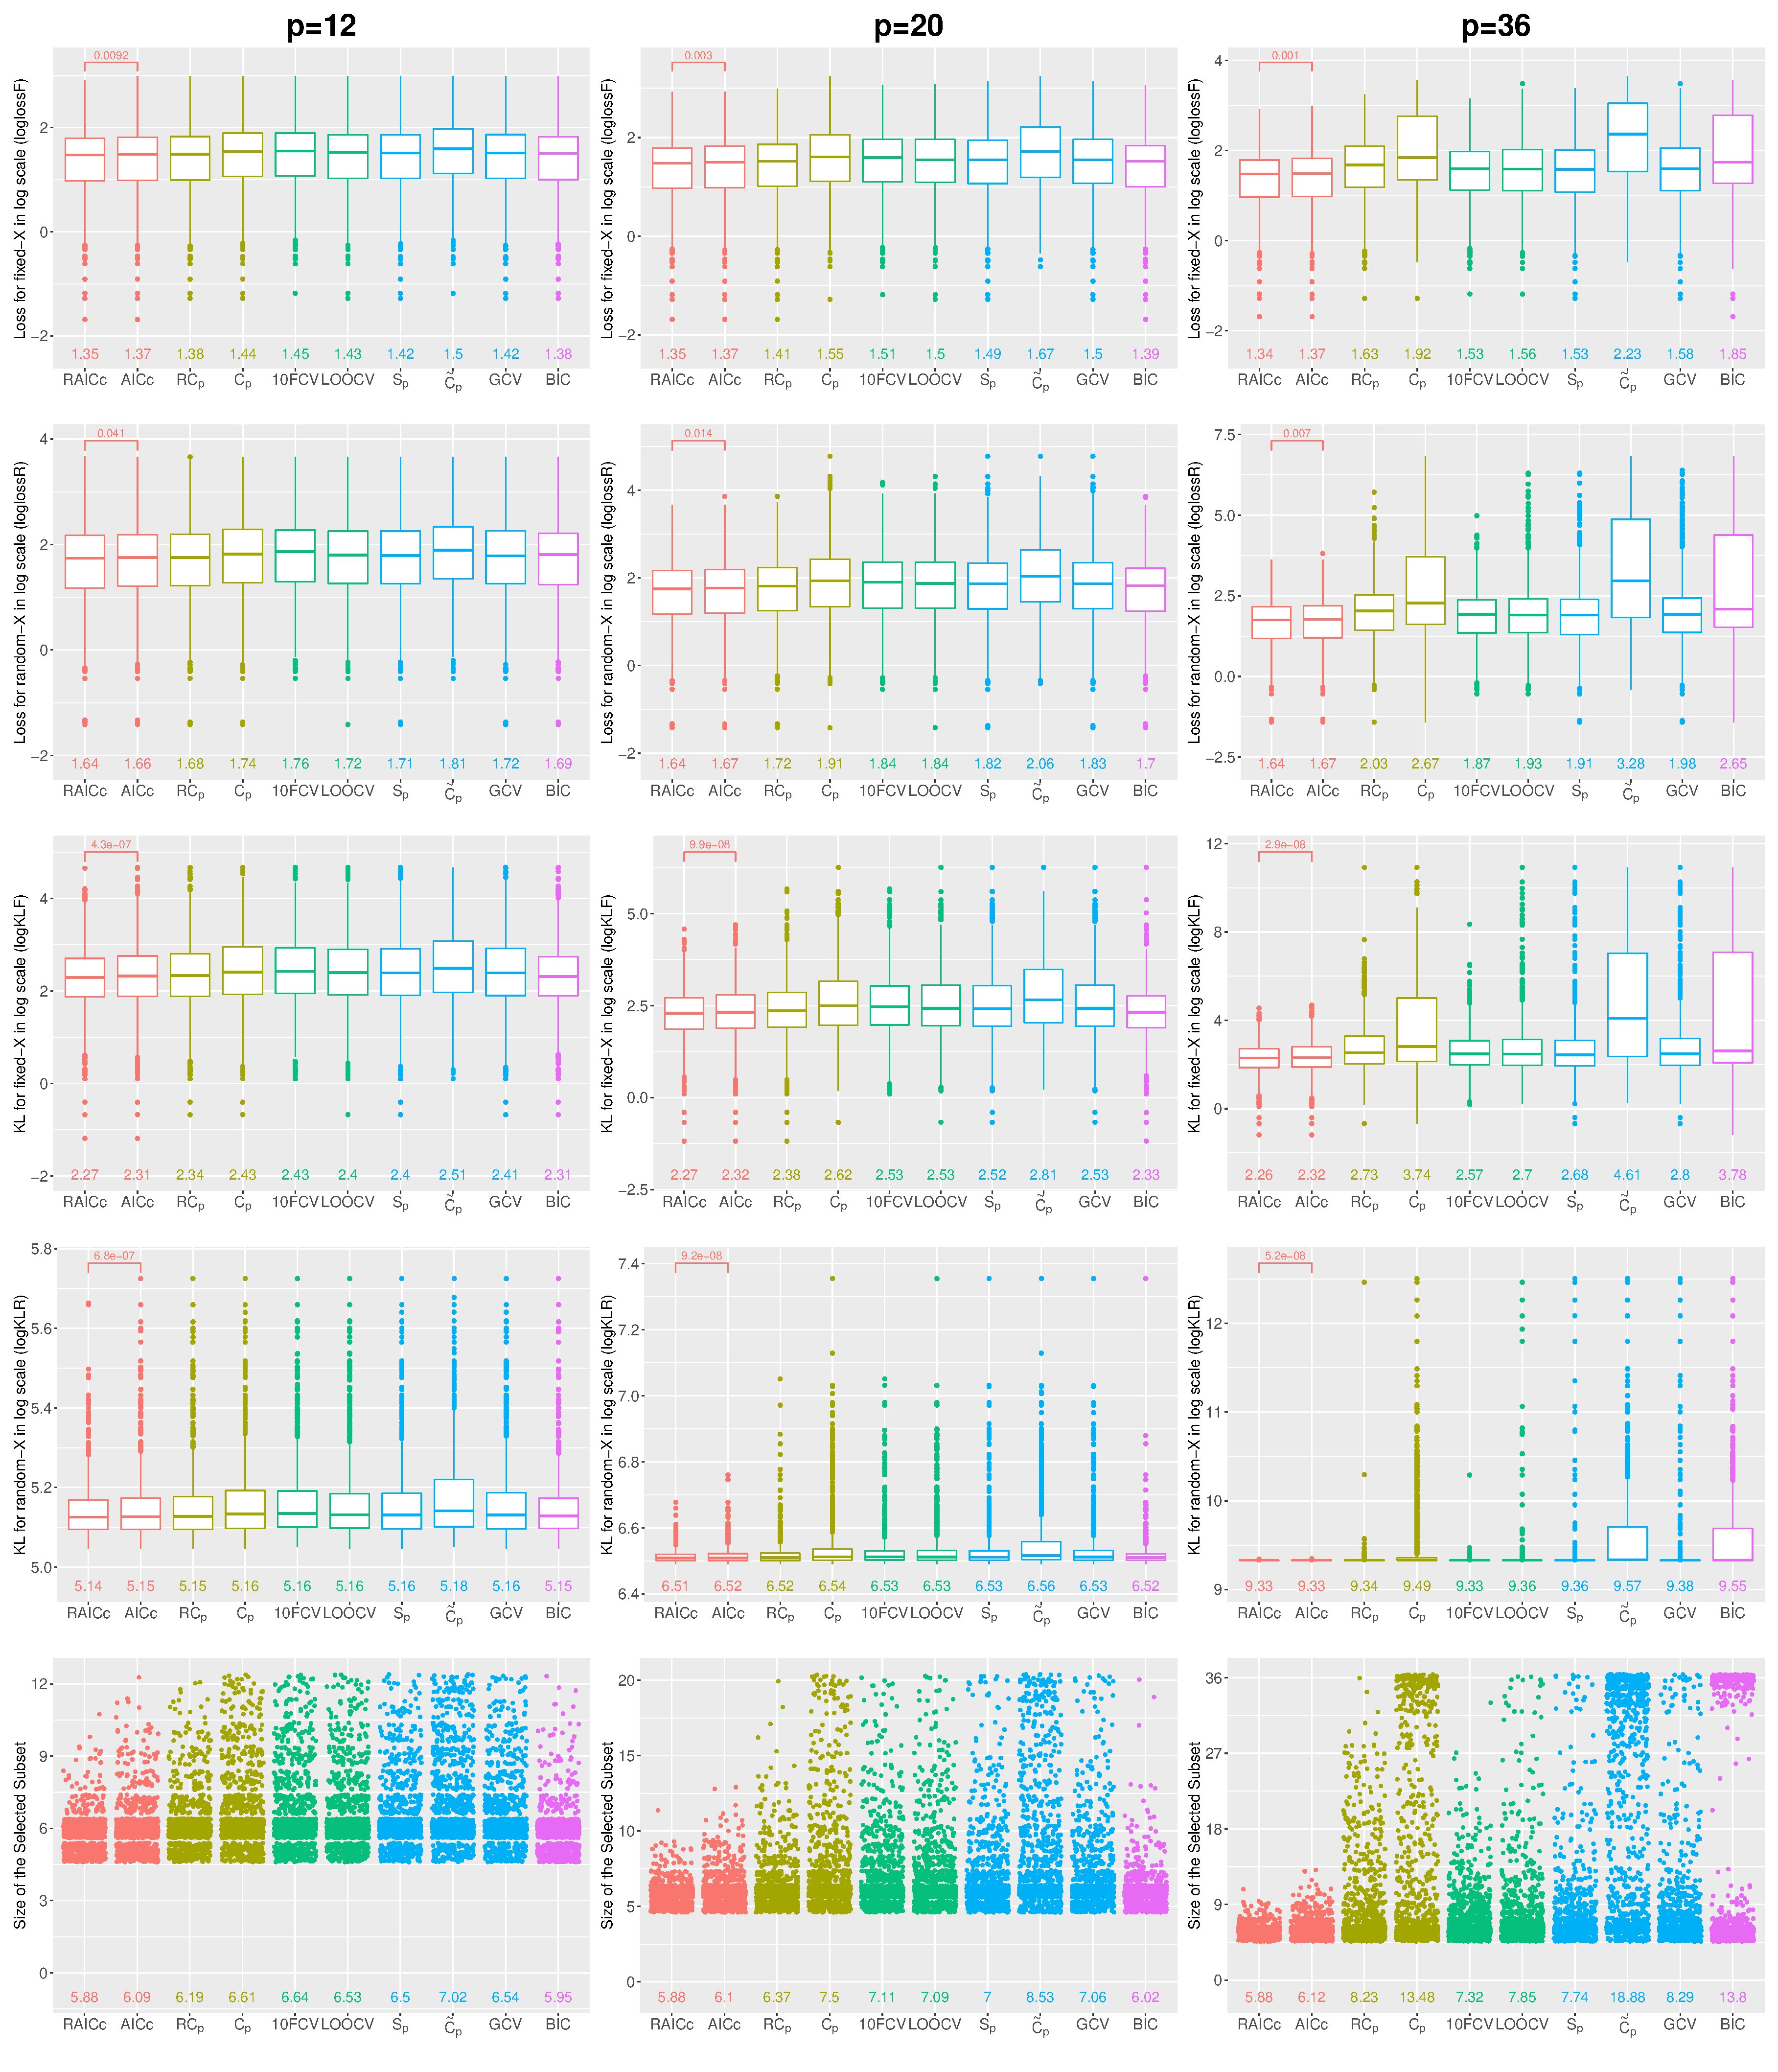
\includegraphics[width=\textwidth]{figures/supplement/fixedx/subset_selection/Sparse-Ex2_n40_hsnr_rho09.eps}
\caption{Variable selection, Fixed-X, Sparse-Ex2, $n=40$, high signal, and $\rho=0.9$.}
\end{figure}
\clearpage
\begin{figure}[!ht]
\centering
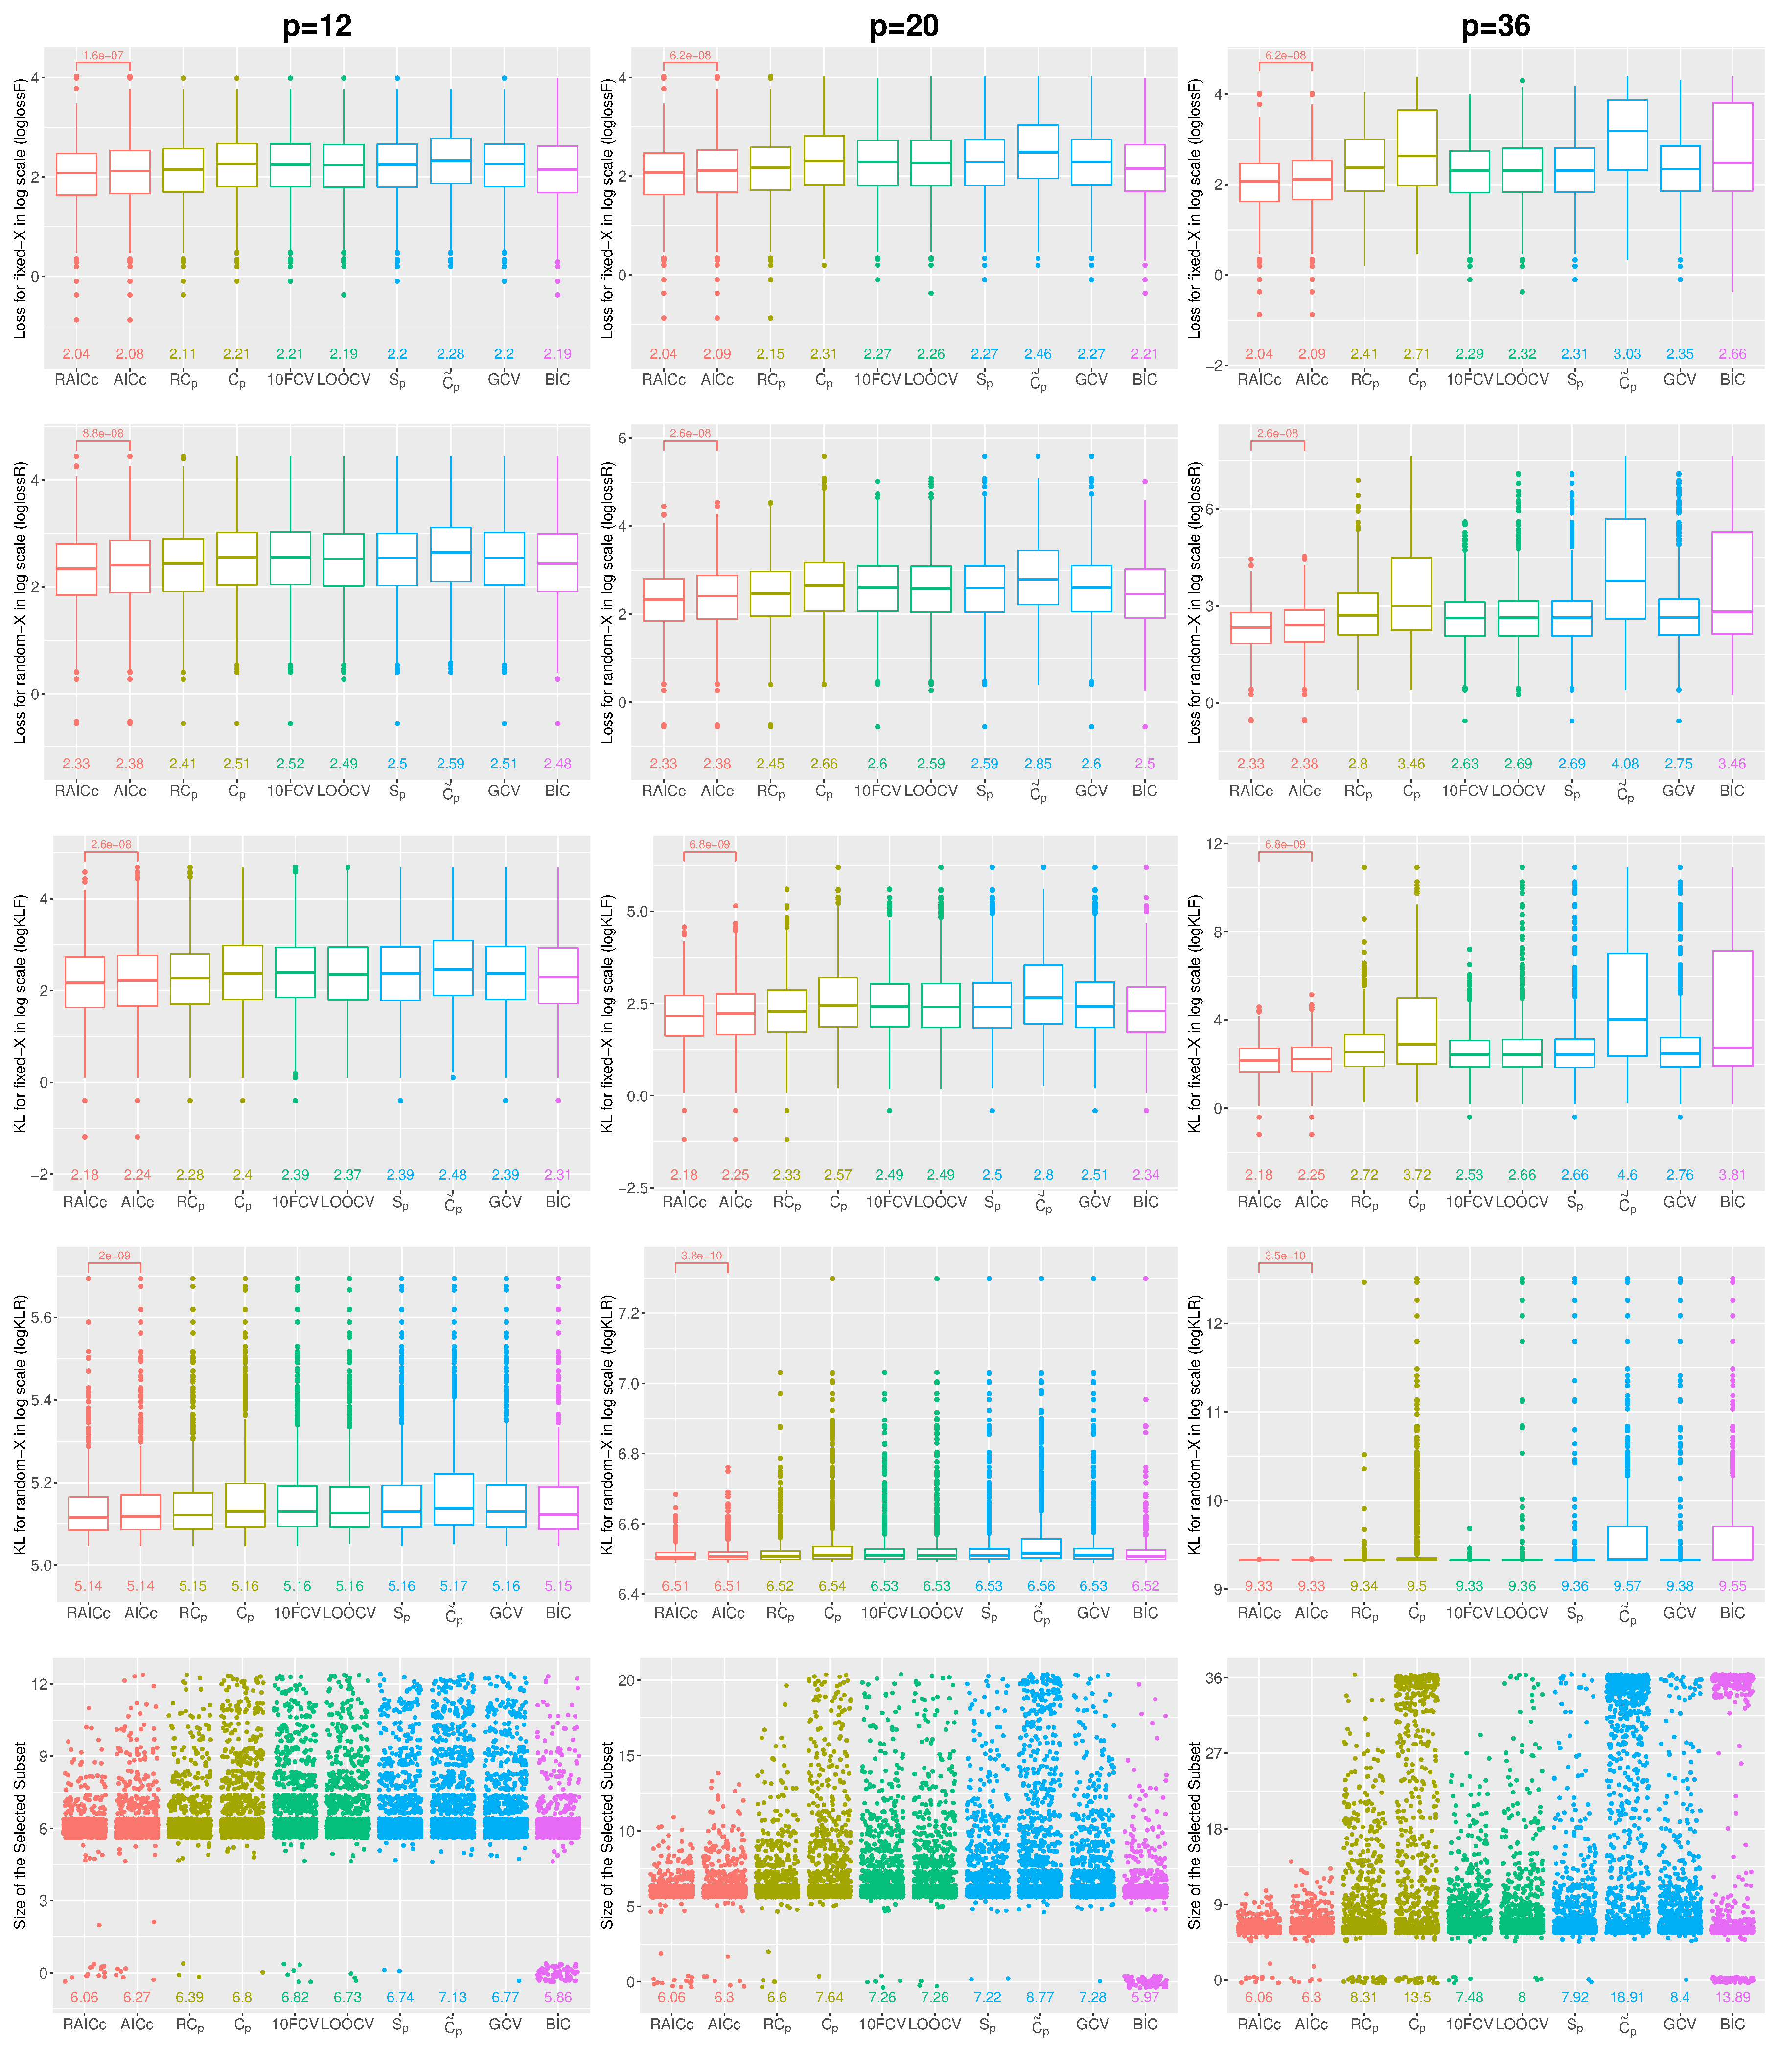
\includegraphics[width=\textwidth]{figures/supplement/fixedx/subset_selection/Sparse-Ex2_n40_msnr_rho0.eps}
\caption{Variable selection, Fixed-X, Sparse-Ex2, $n=40$, medium signal, and $\rho=0$.}
\end{figure}
\clearpage
\begin{figure}[!ht]
\centering
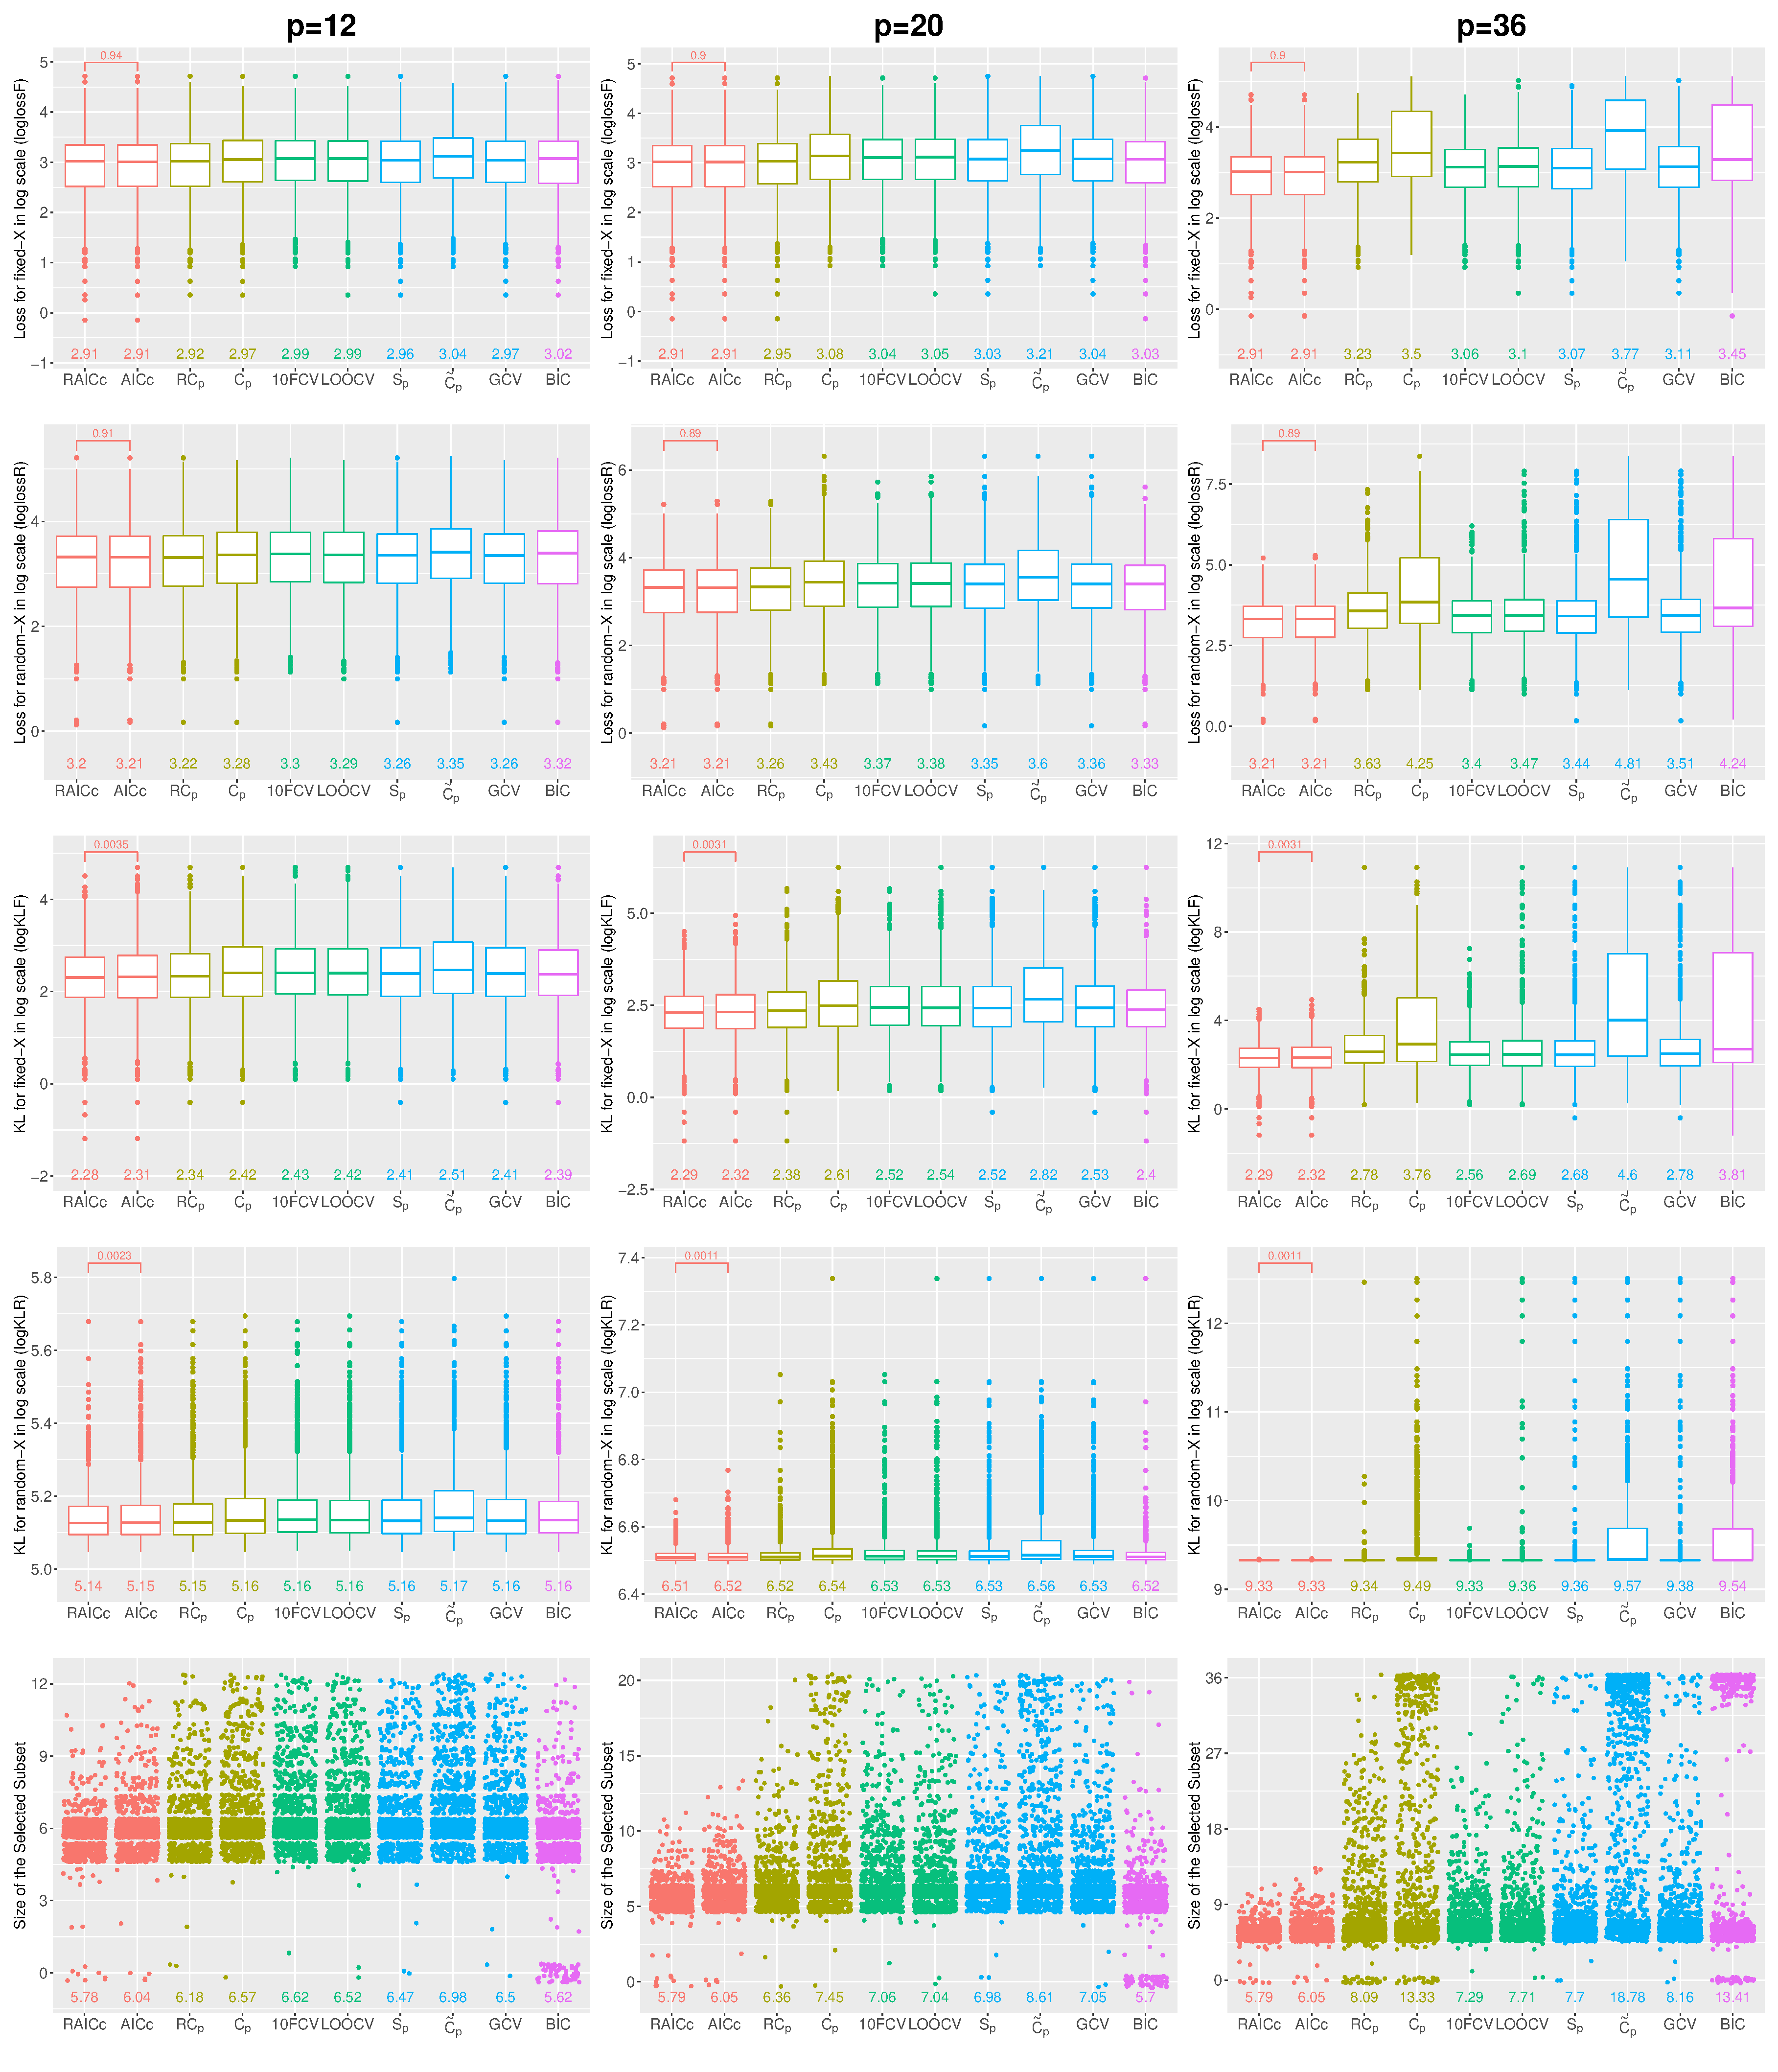
\includegraphics[width=\textwidth]{figures/supplement/fixedx/subset_selection/Sparse-Ex2_n40_msnr_rho05.eps}
\caption{Variable selection, Fixed-X, Sparse-Ex2, $n=40$, medium signal, and $\rho=0.5$.}
\end{figure}
\clearpage
\begin{figure}[!ht]
\centering
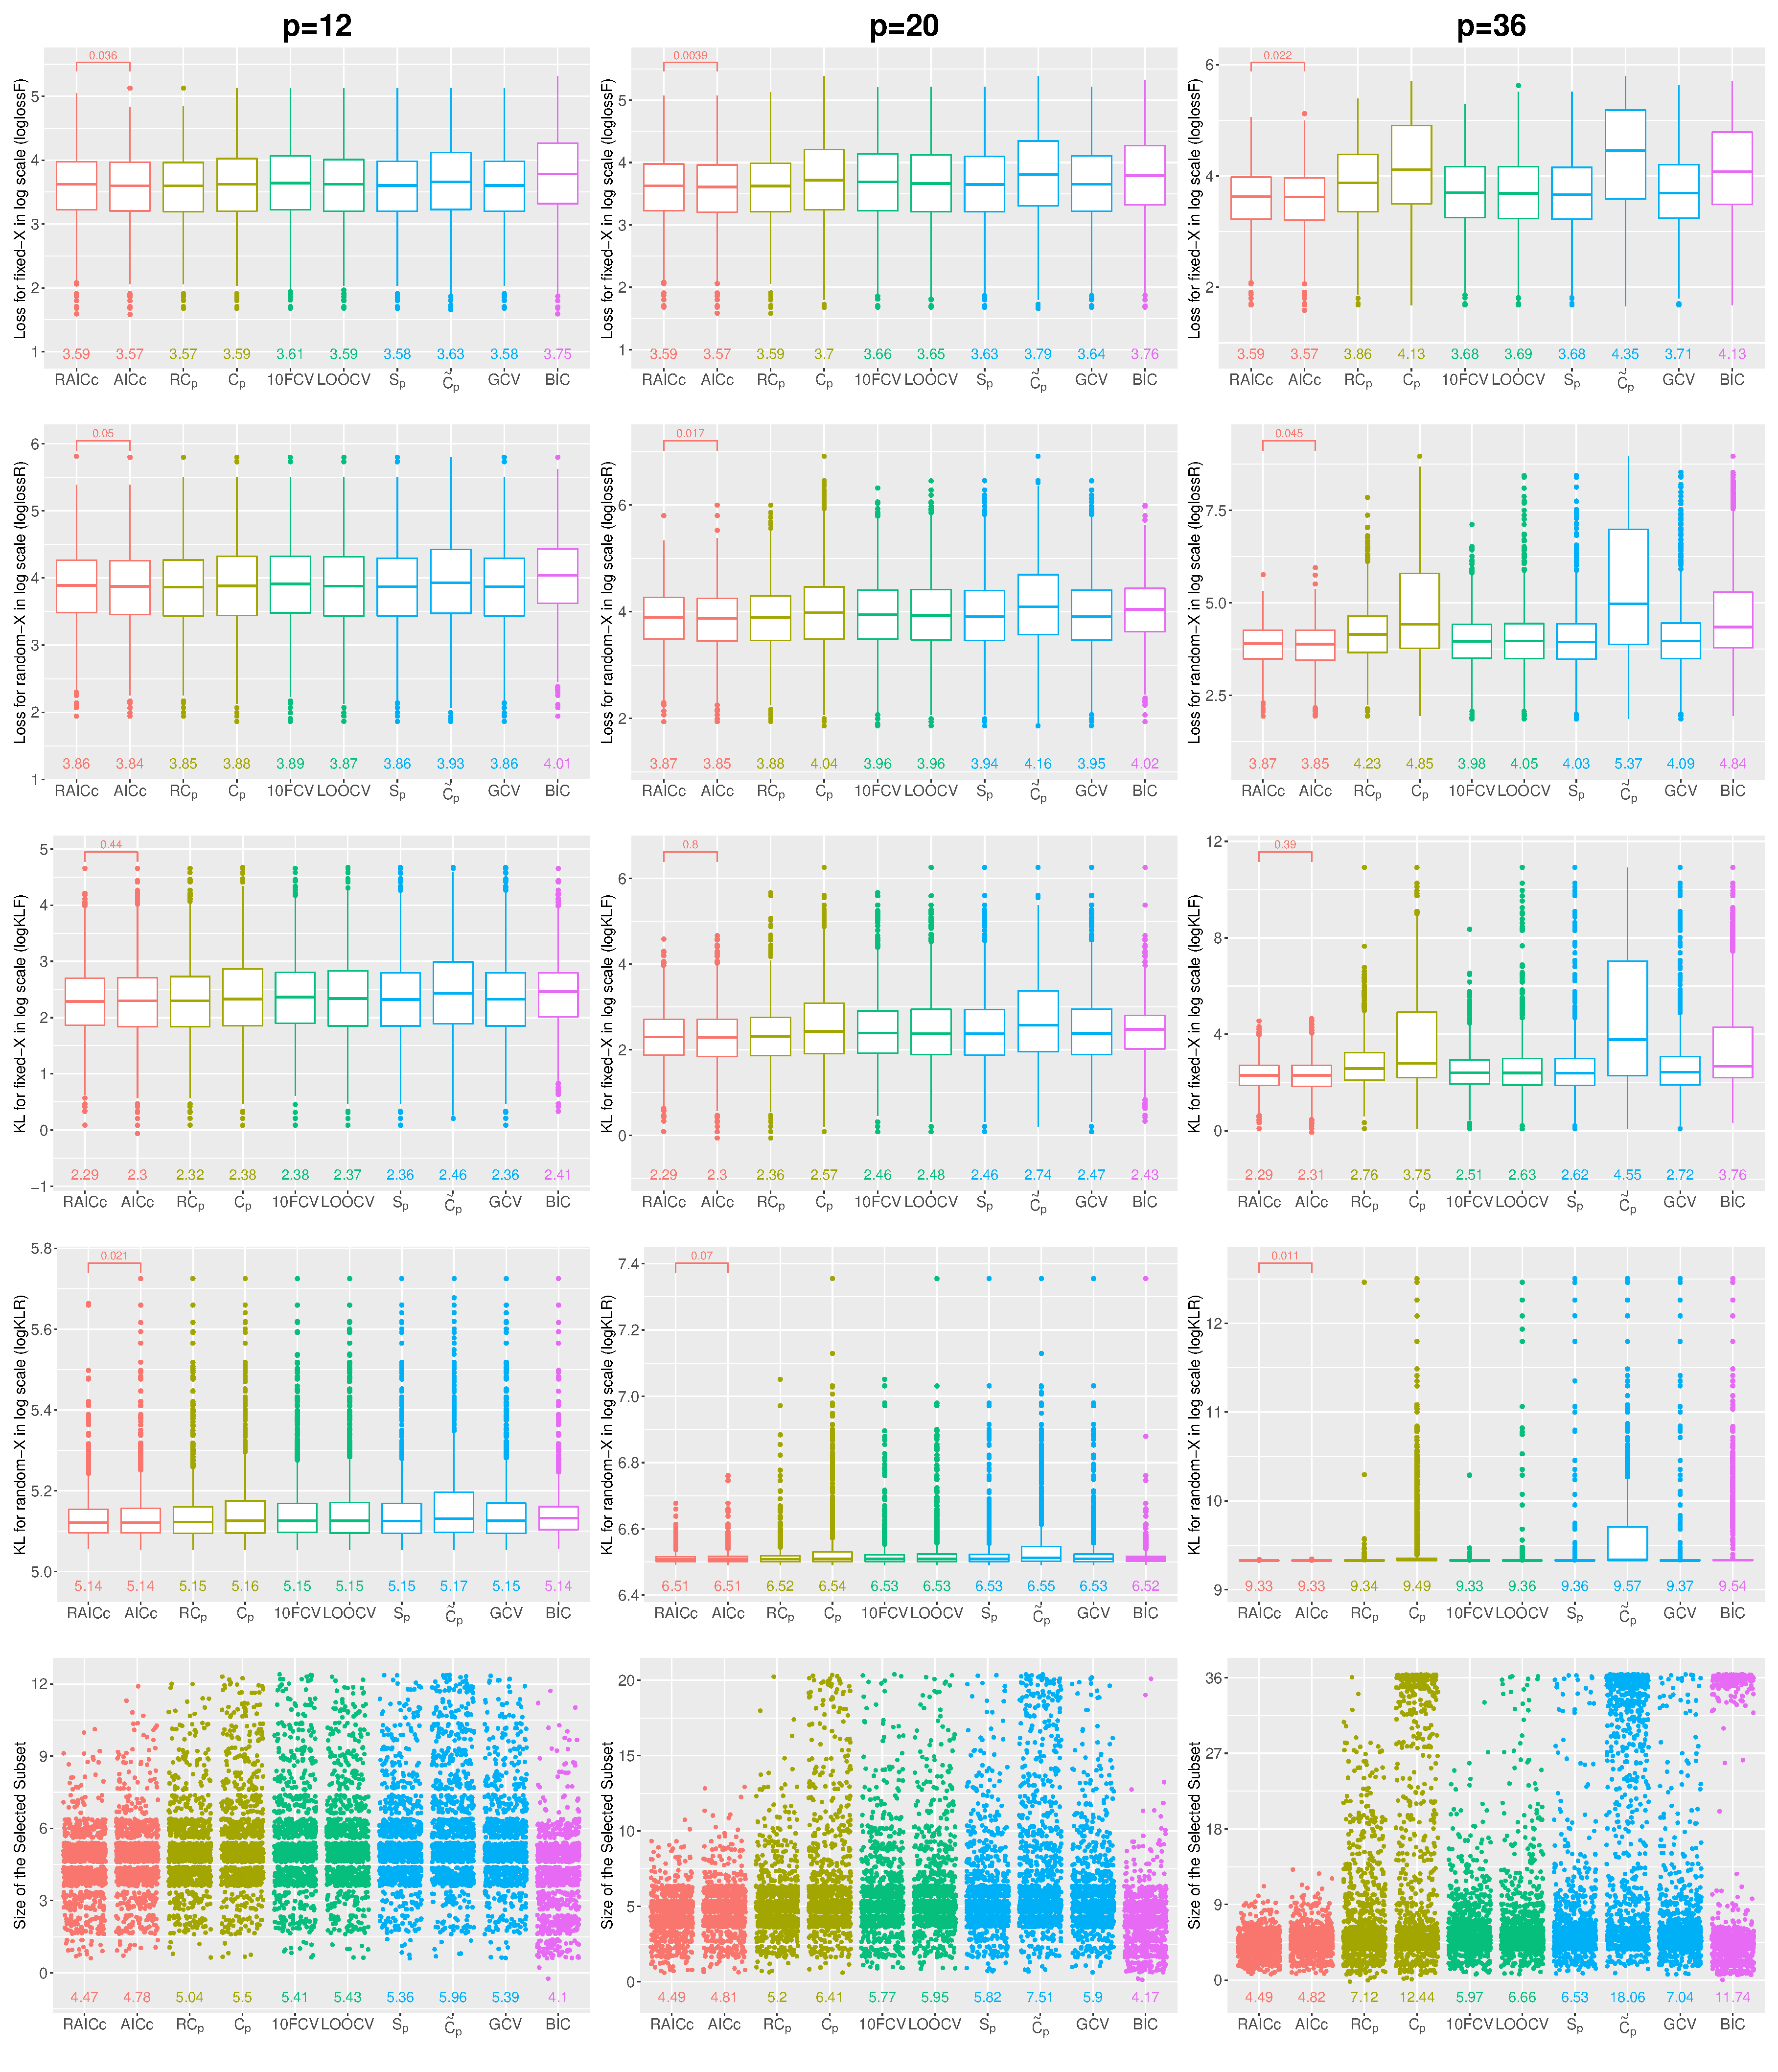
\includegraphics[width=\textwidth]{figures/supplement/fixedx/subset_selection/Sparse-Ex2_n40_msnr_rho09.eps}
\caption{Variable selection, Fixed-X, Sparse-Ex2, $n=40$, medium signal, and $\rho=0.9$.}
\end{figure}
\clearpage
\begin{figure}[!ht]
\centering
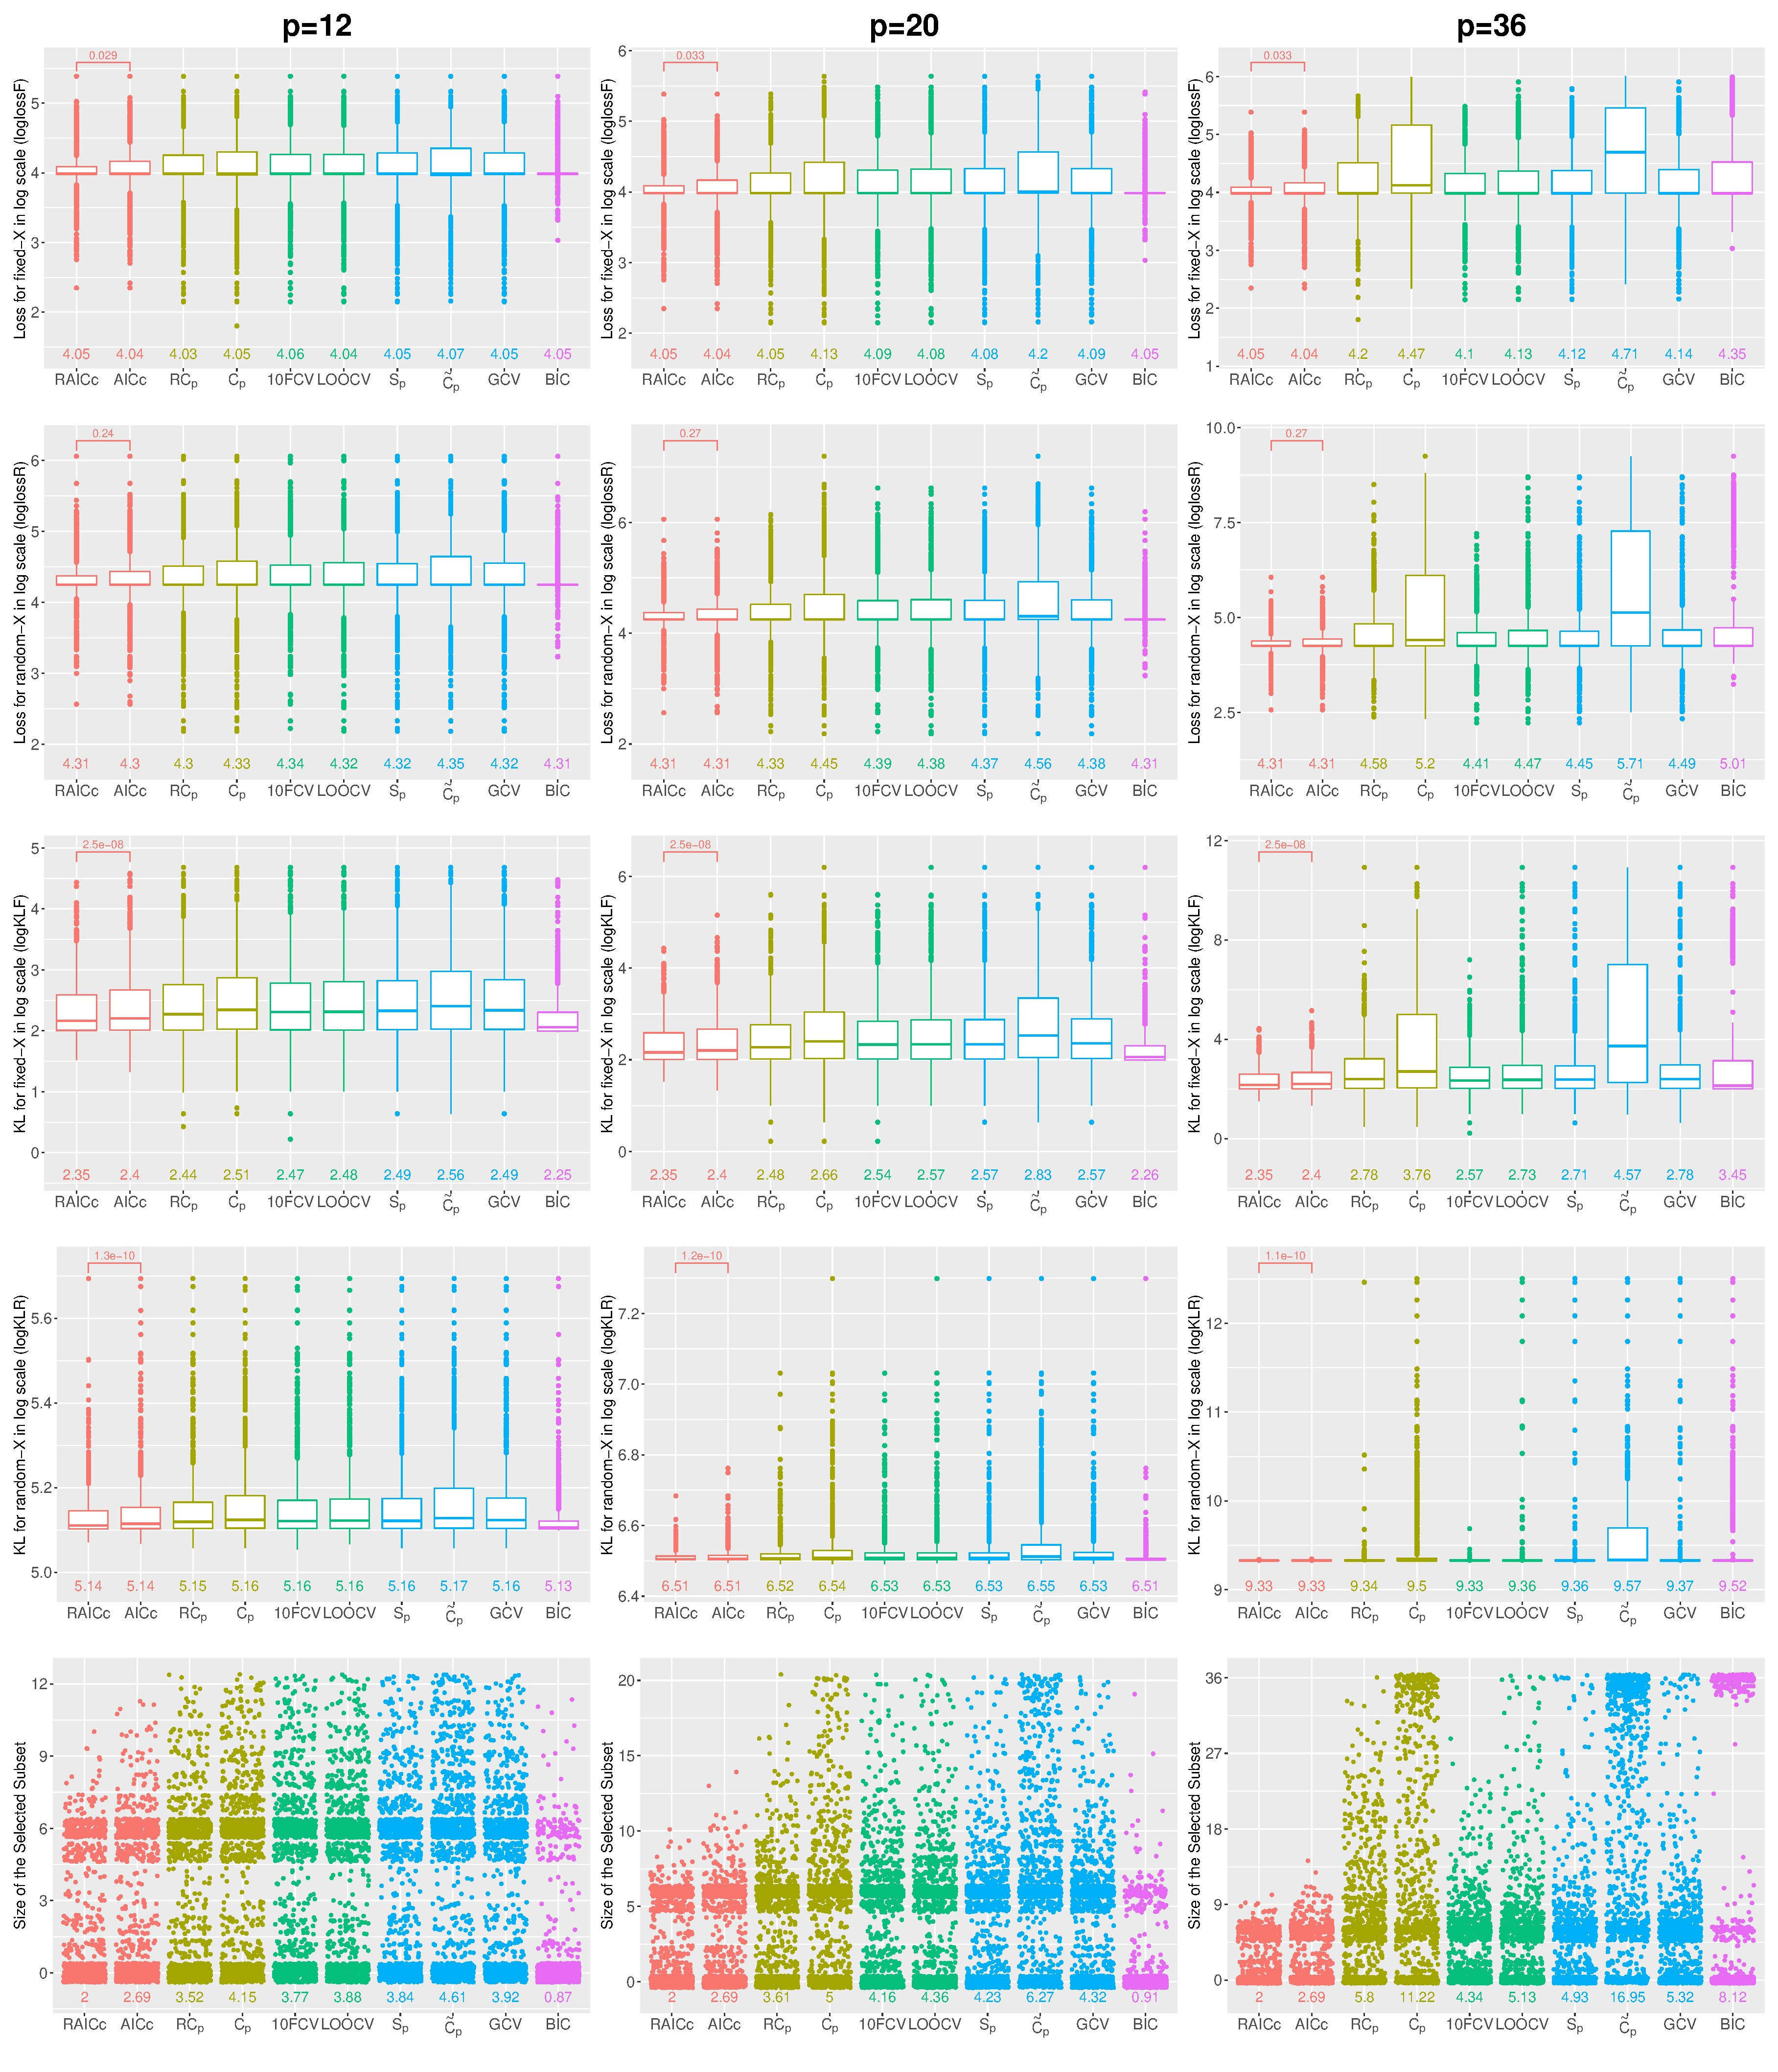
\includegraphics[width=\textwidth]{figures/supplement/fixedx/subset_selection/Sparse-Ex2_n40_lsnr_rho0.eps}
\caption{Variable selection, Fixed-X, Sparse-Ex2, $n=40$, low signal, and $\rho=0$.}
\end{figure}
\clearpage
\begin{figure}[!ht]
\centering
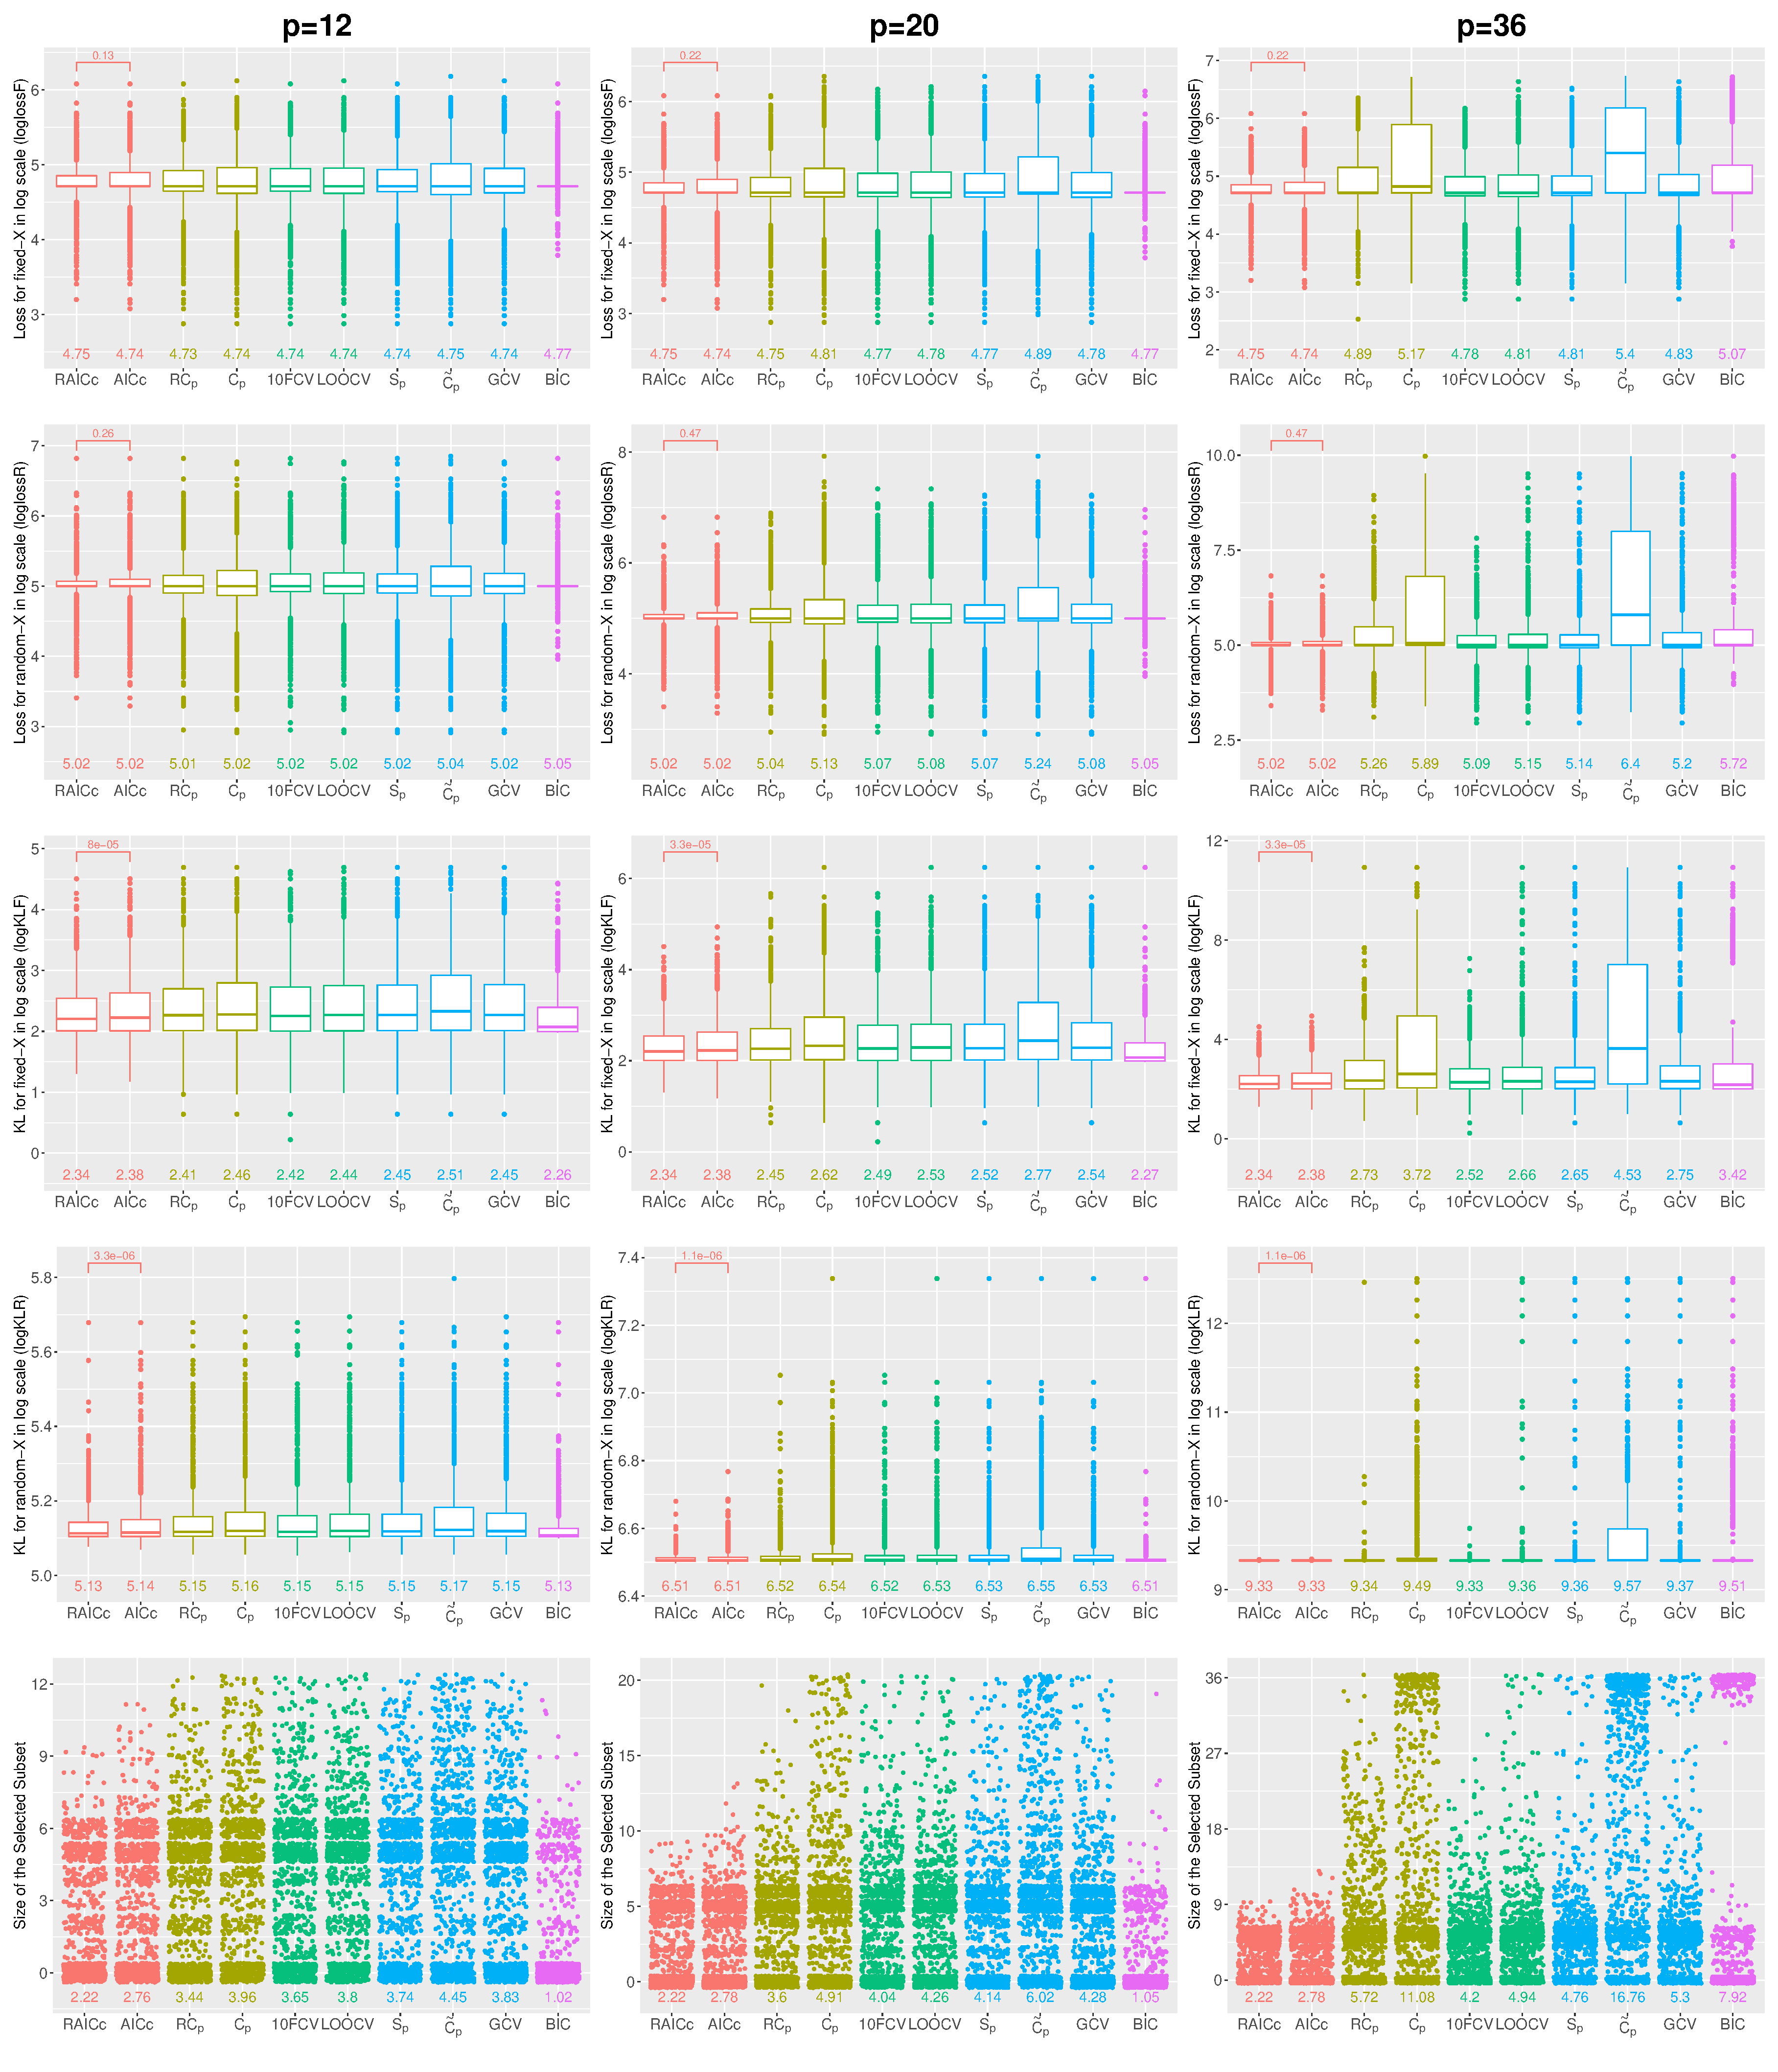
\includegraphics[width=\textwidth]{figures/supplement/fixedx/subset_selection/Sparse-Ex2_n40_lsnr_rho05.eps}
\caption{Variable selection, Fixed-X, Sparse-Ex2, $n=40$, low signal, and $\rho=0.5$.}
\end{figure}
\clearpage
\begin{figure}[!ht]
\centering
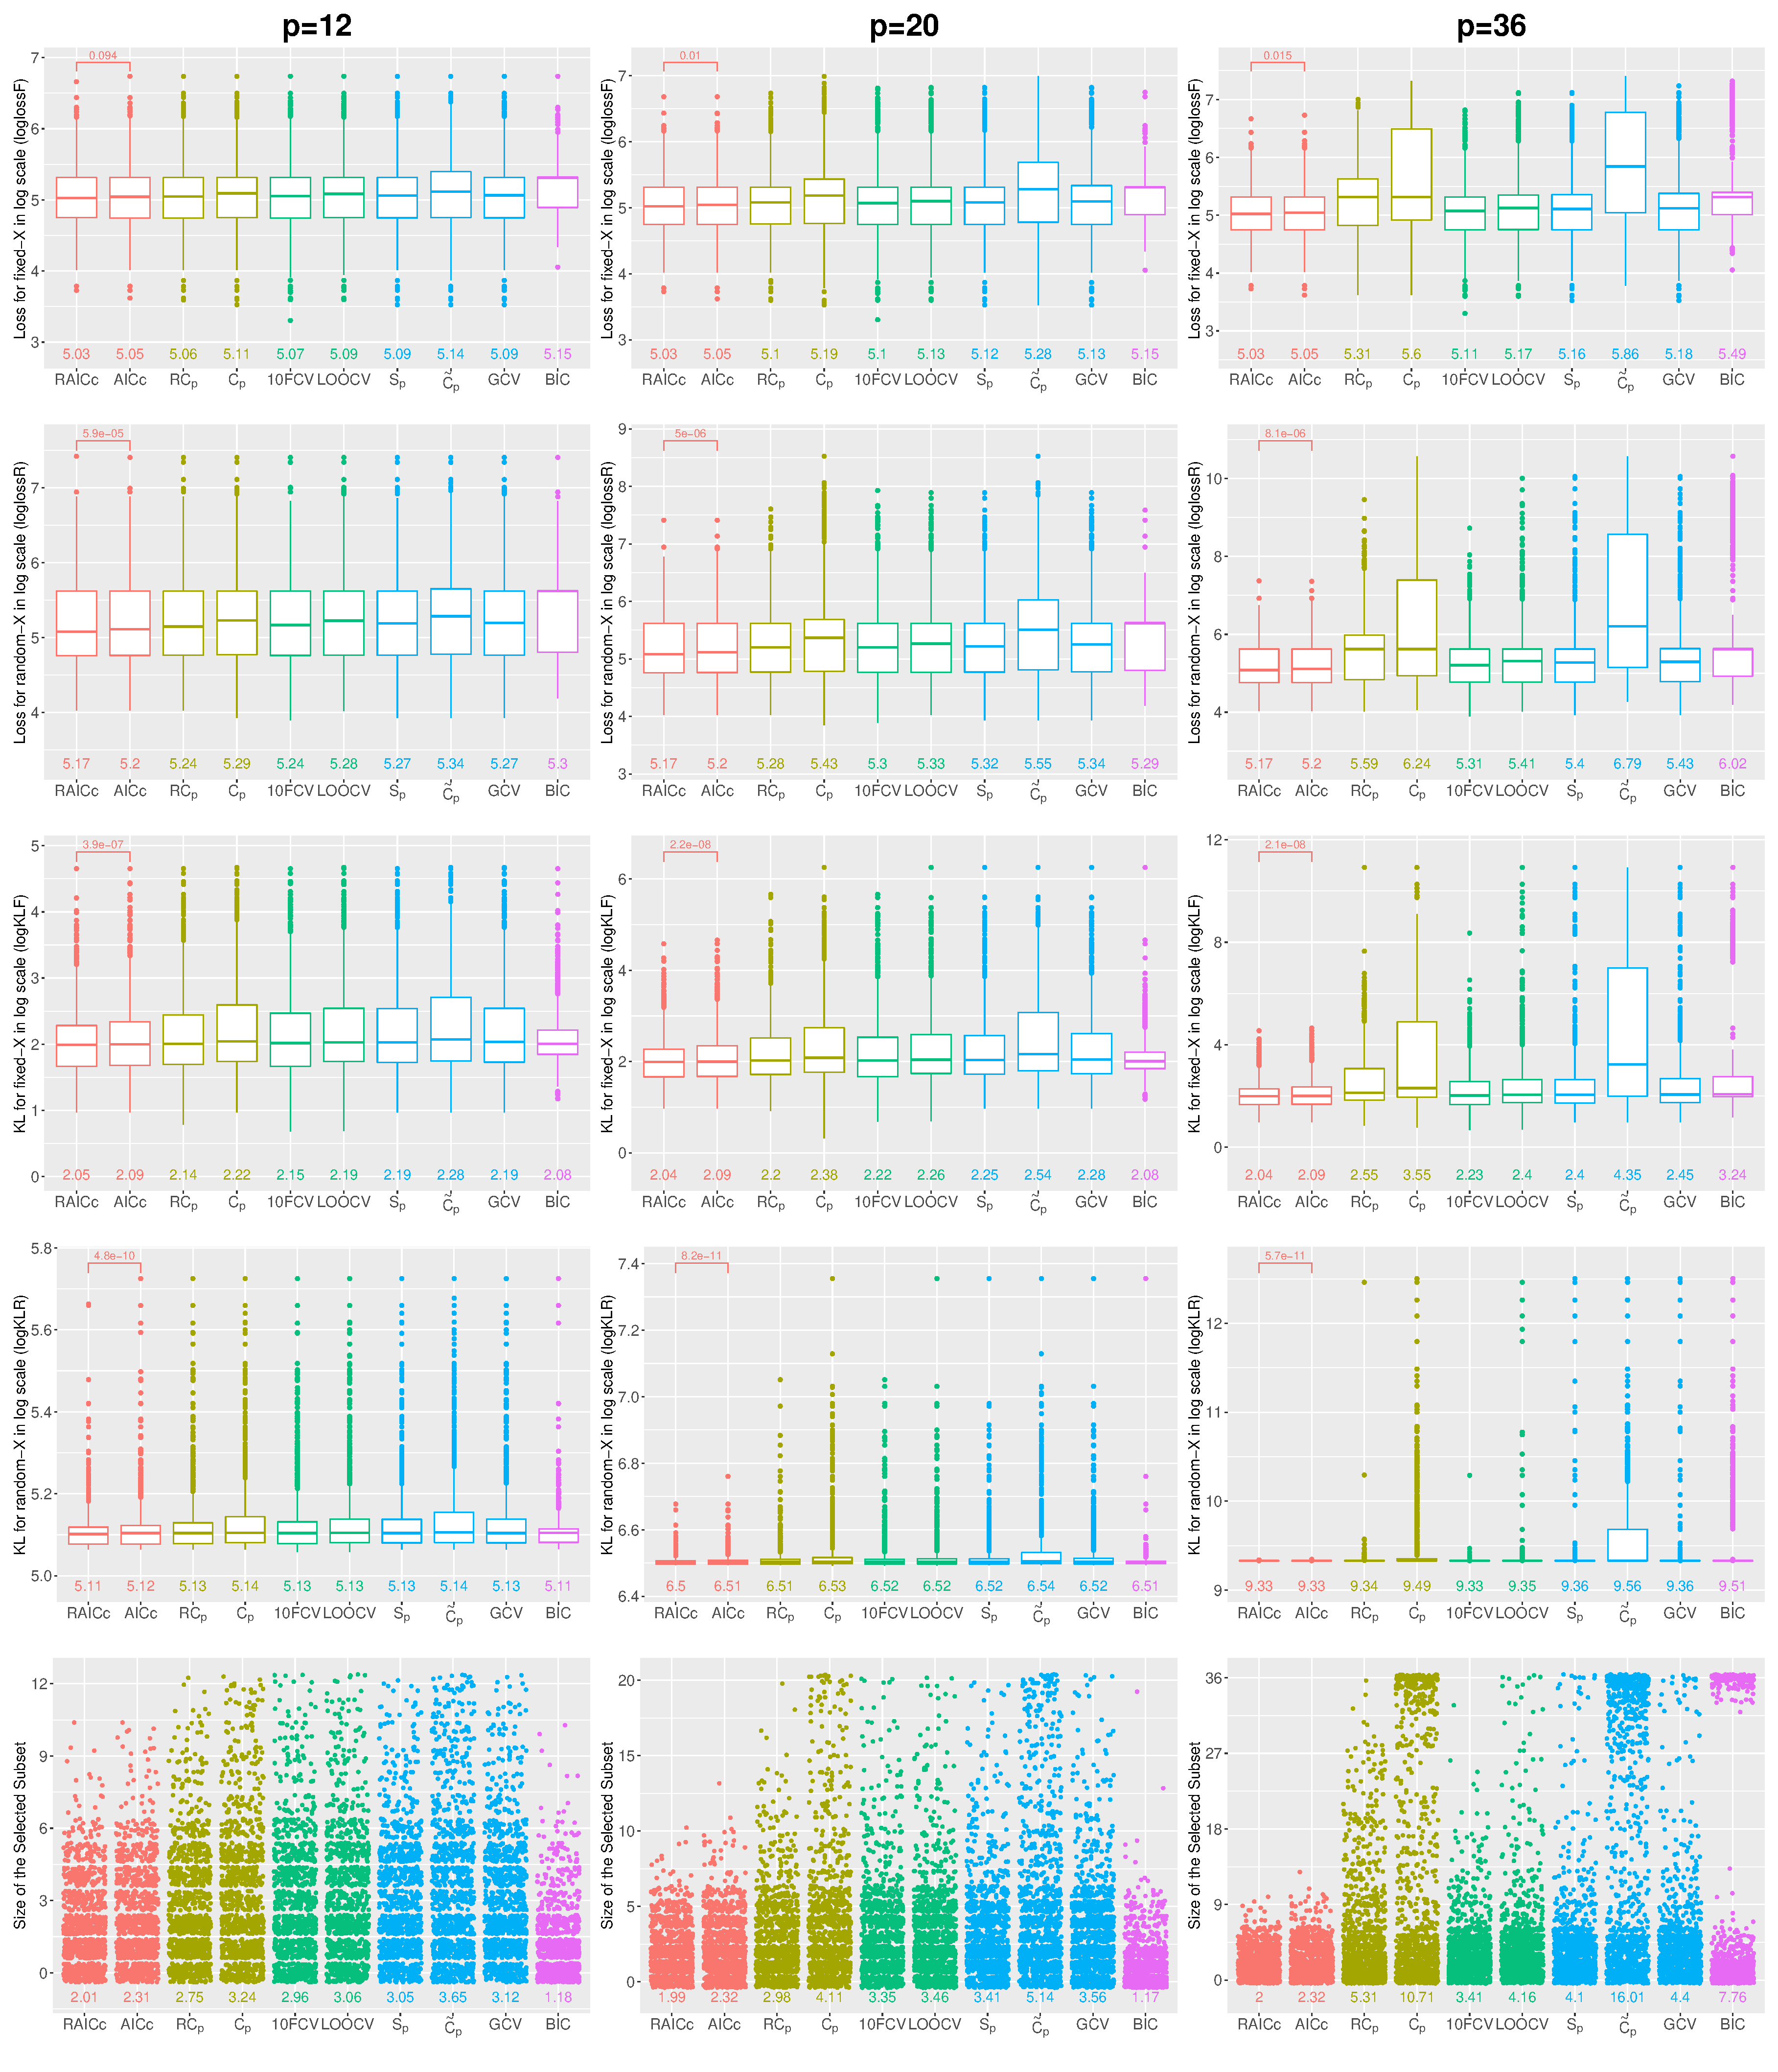
\includegraphics[width=\textwidth]{figures/supplement/fixedx/subset_selection/Sparse-Ex2_n40_lsnr_rho09.eps}
\caption{Variable selection, Fixed-X, Sparse-Ex2, $n=40$, low signal, and $\rho=0.9$.}
\end{figure}
\clearpage
\begin{figure}[!ht]
\centering
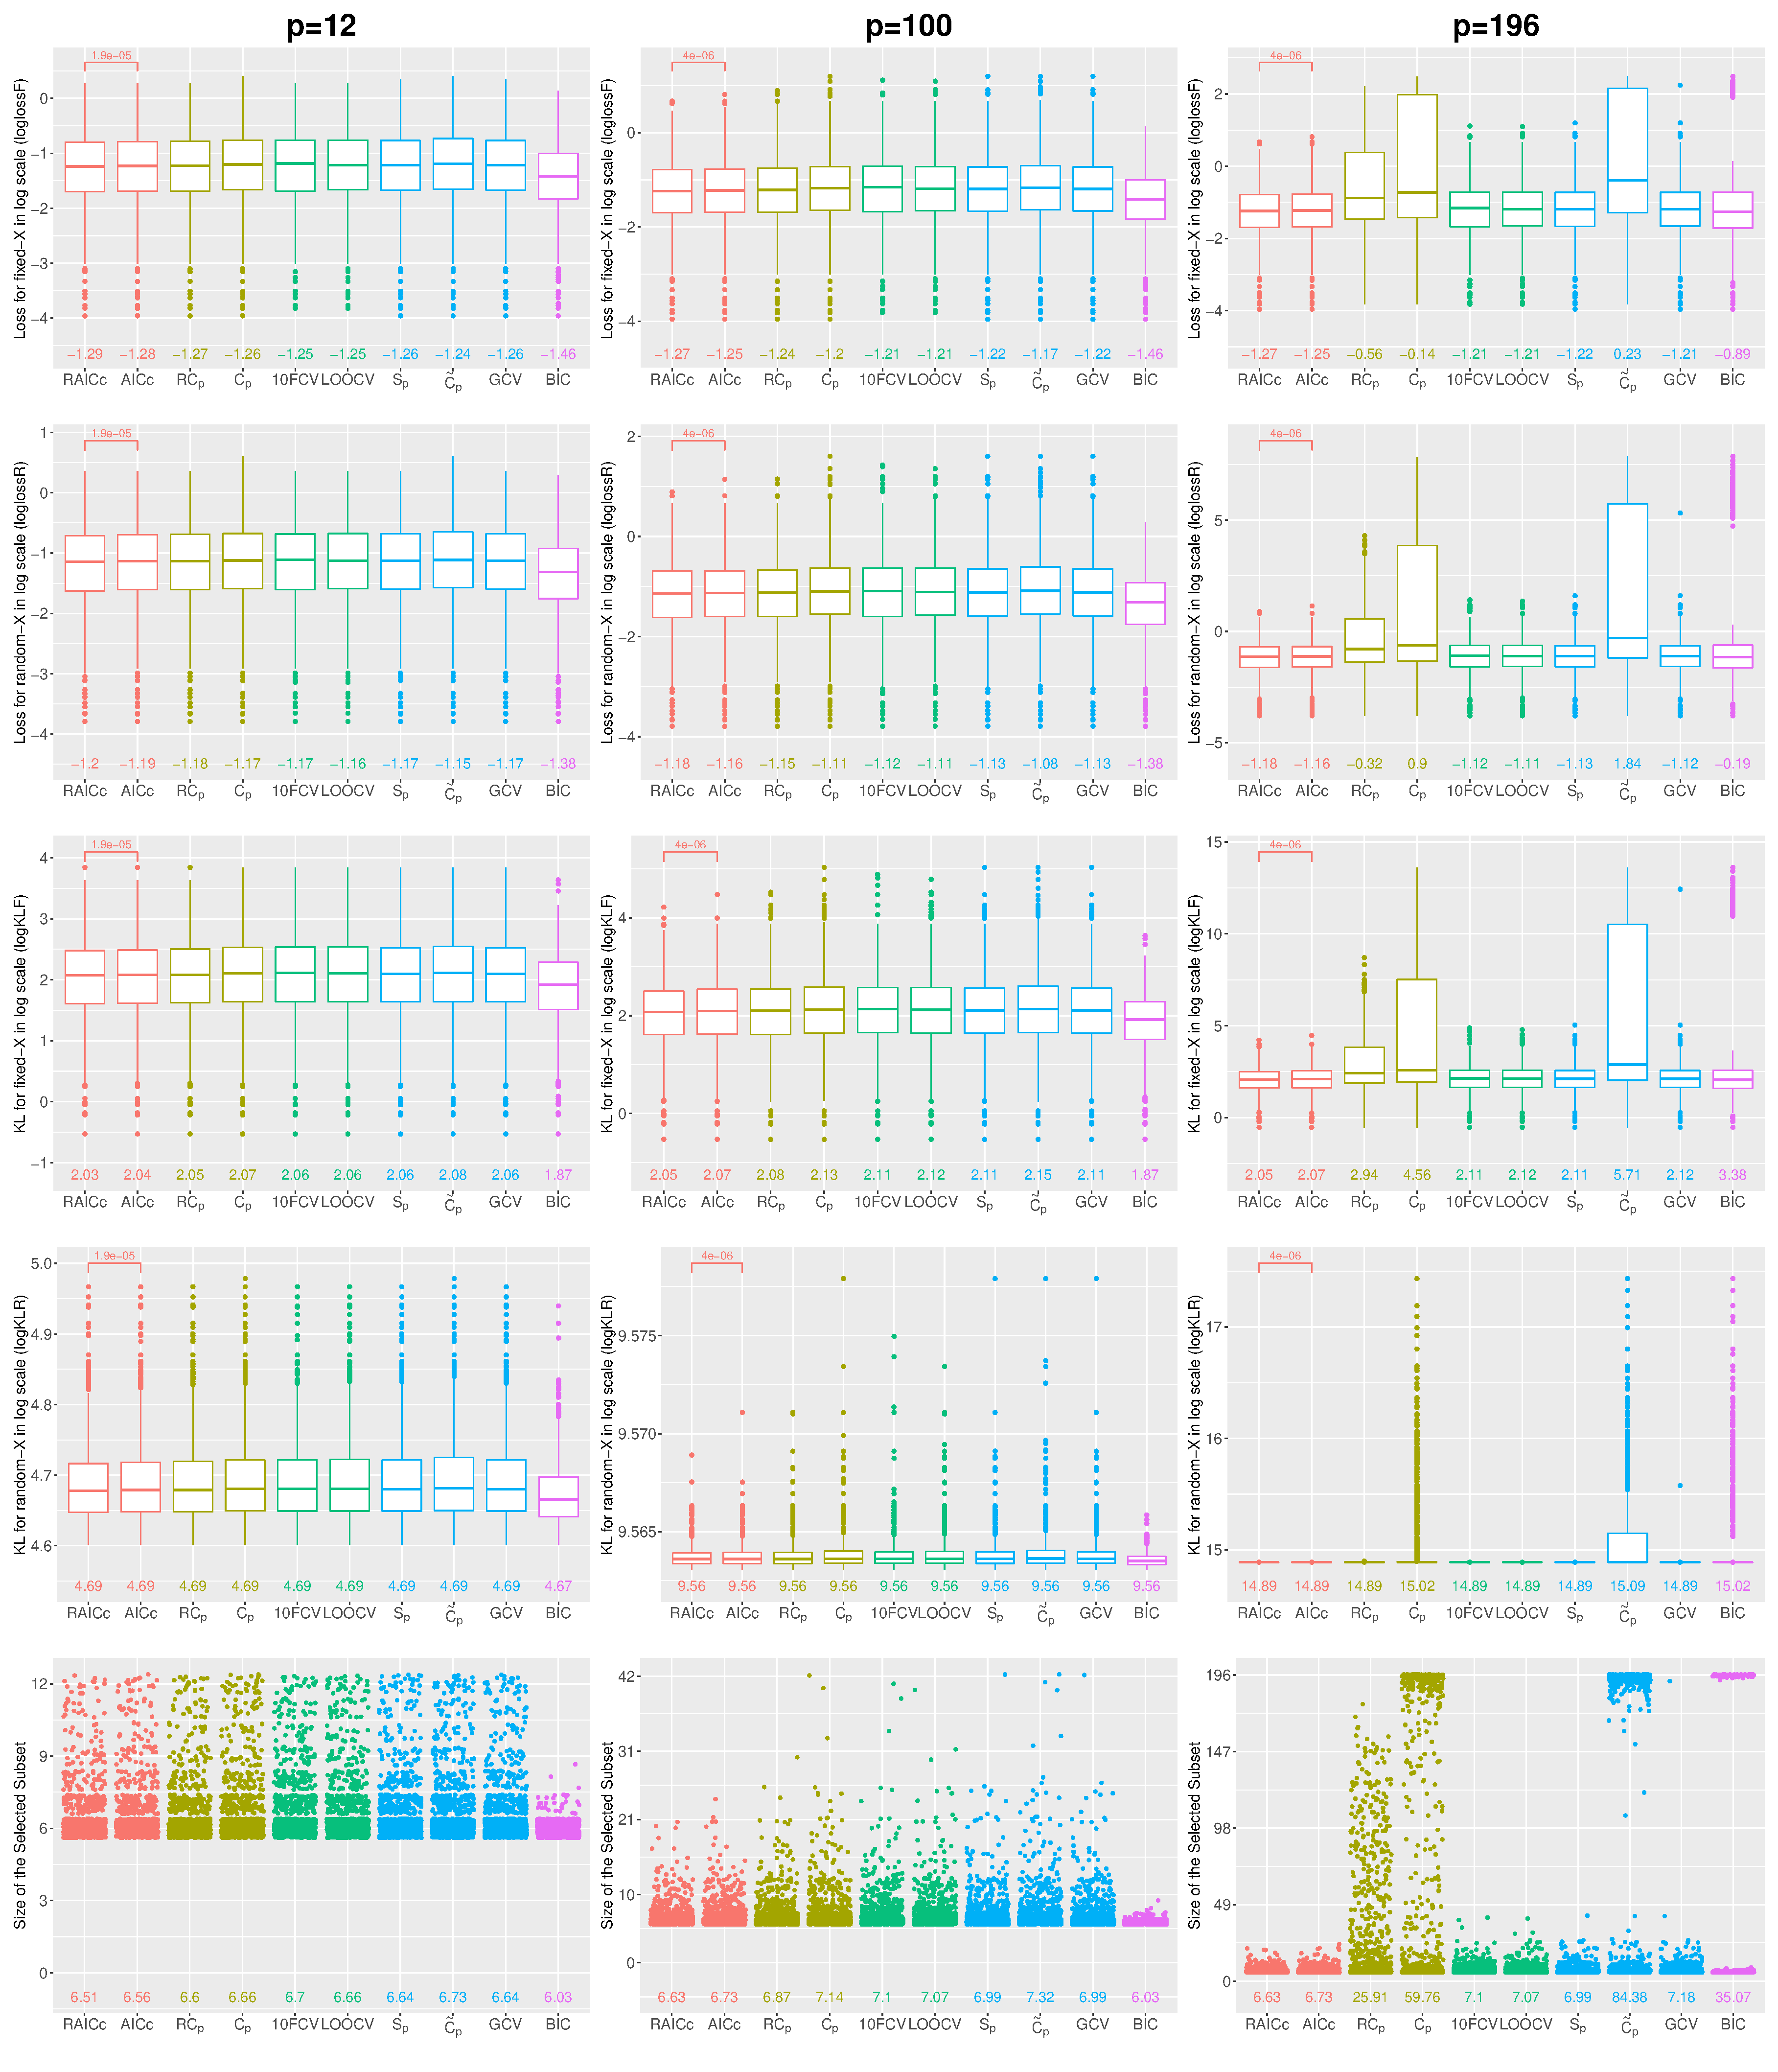
\includegraphics[width=\textwidth]{figures/supplement/fixedx/subset_selection/Sparse-Ex2_n200_hsnr_rho0.eps}
\caption{Variable selection, Fixed-X, Sparse-Ex2, $n=200$, high signal, and $\rho=0$.}
\end{figure}
\clearpage
\begin{figure}[!ht]
\centering
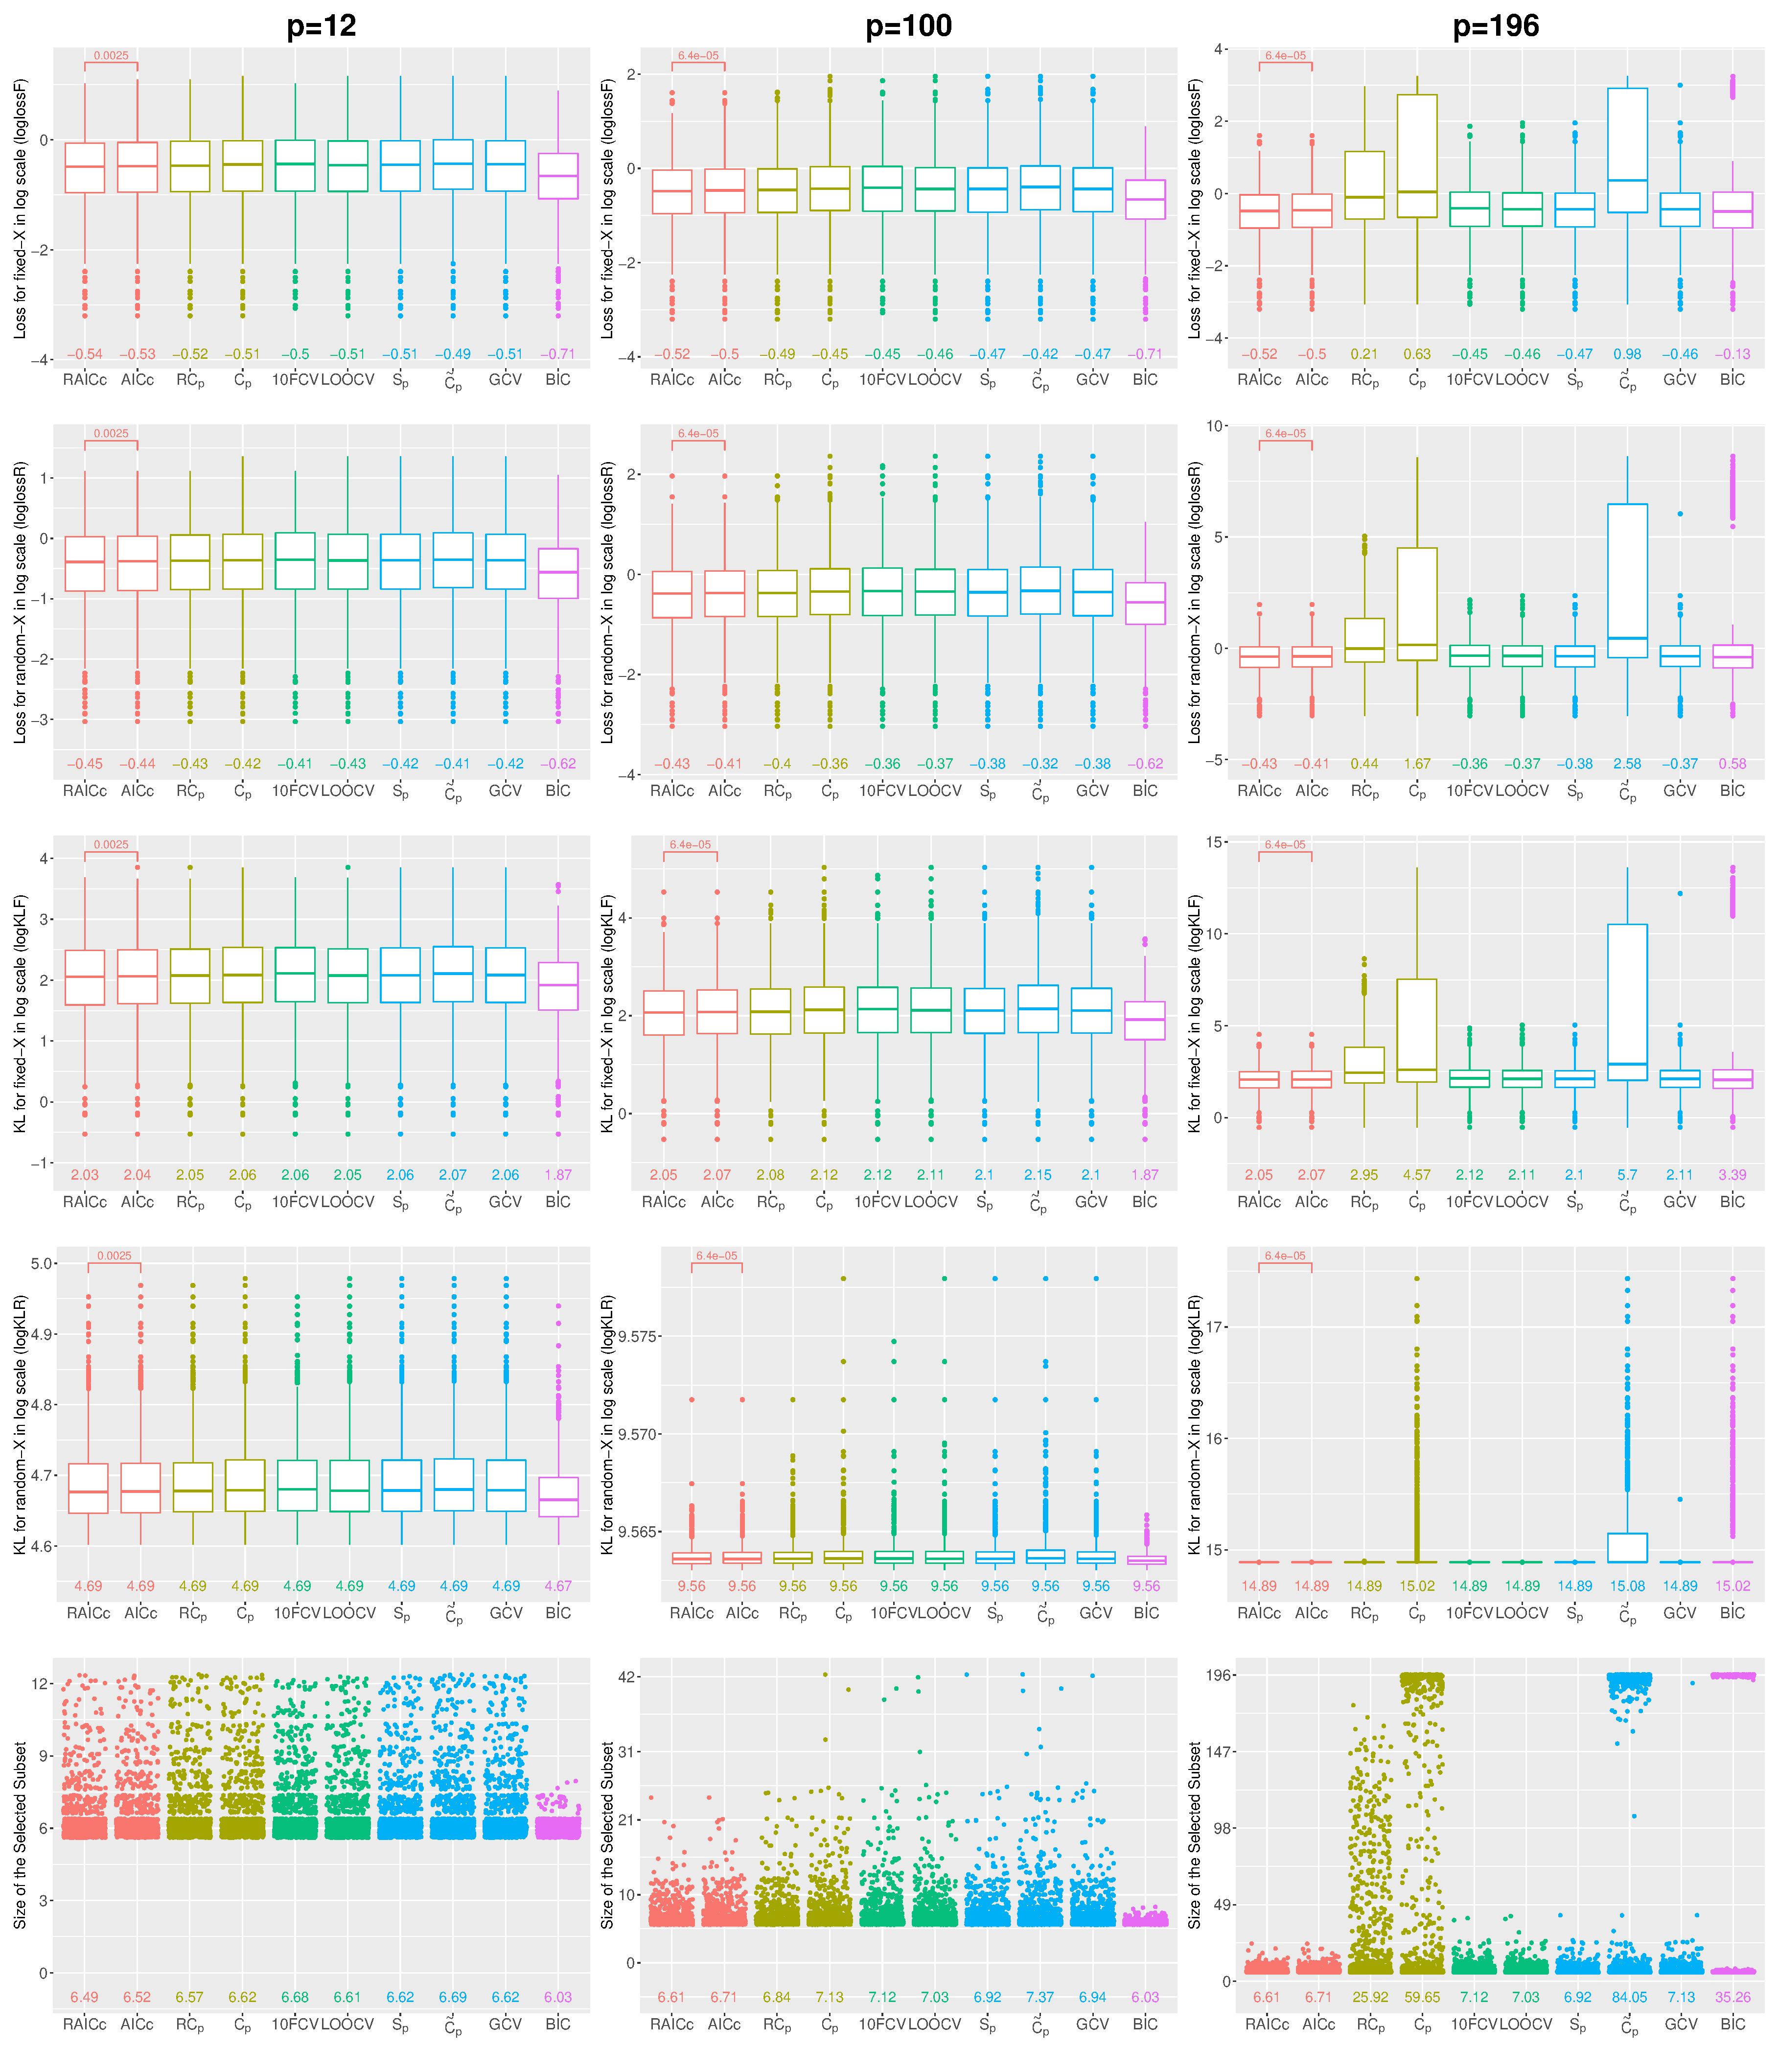
\includegraphics[width=\textwidth]{figures/supplement/fixedx/subset_selection/Sparse-Ex2_n200_hsnr_rho05.eps}
\caption{Variable selection, Fixed-X, Sparse-Ex2, $n=200$, high signal, and $\rho=0.5$.}
\end{figure}
\clearpage
\begin{figure}[!ht]
\centering
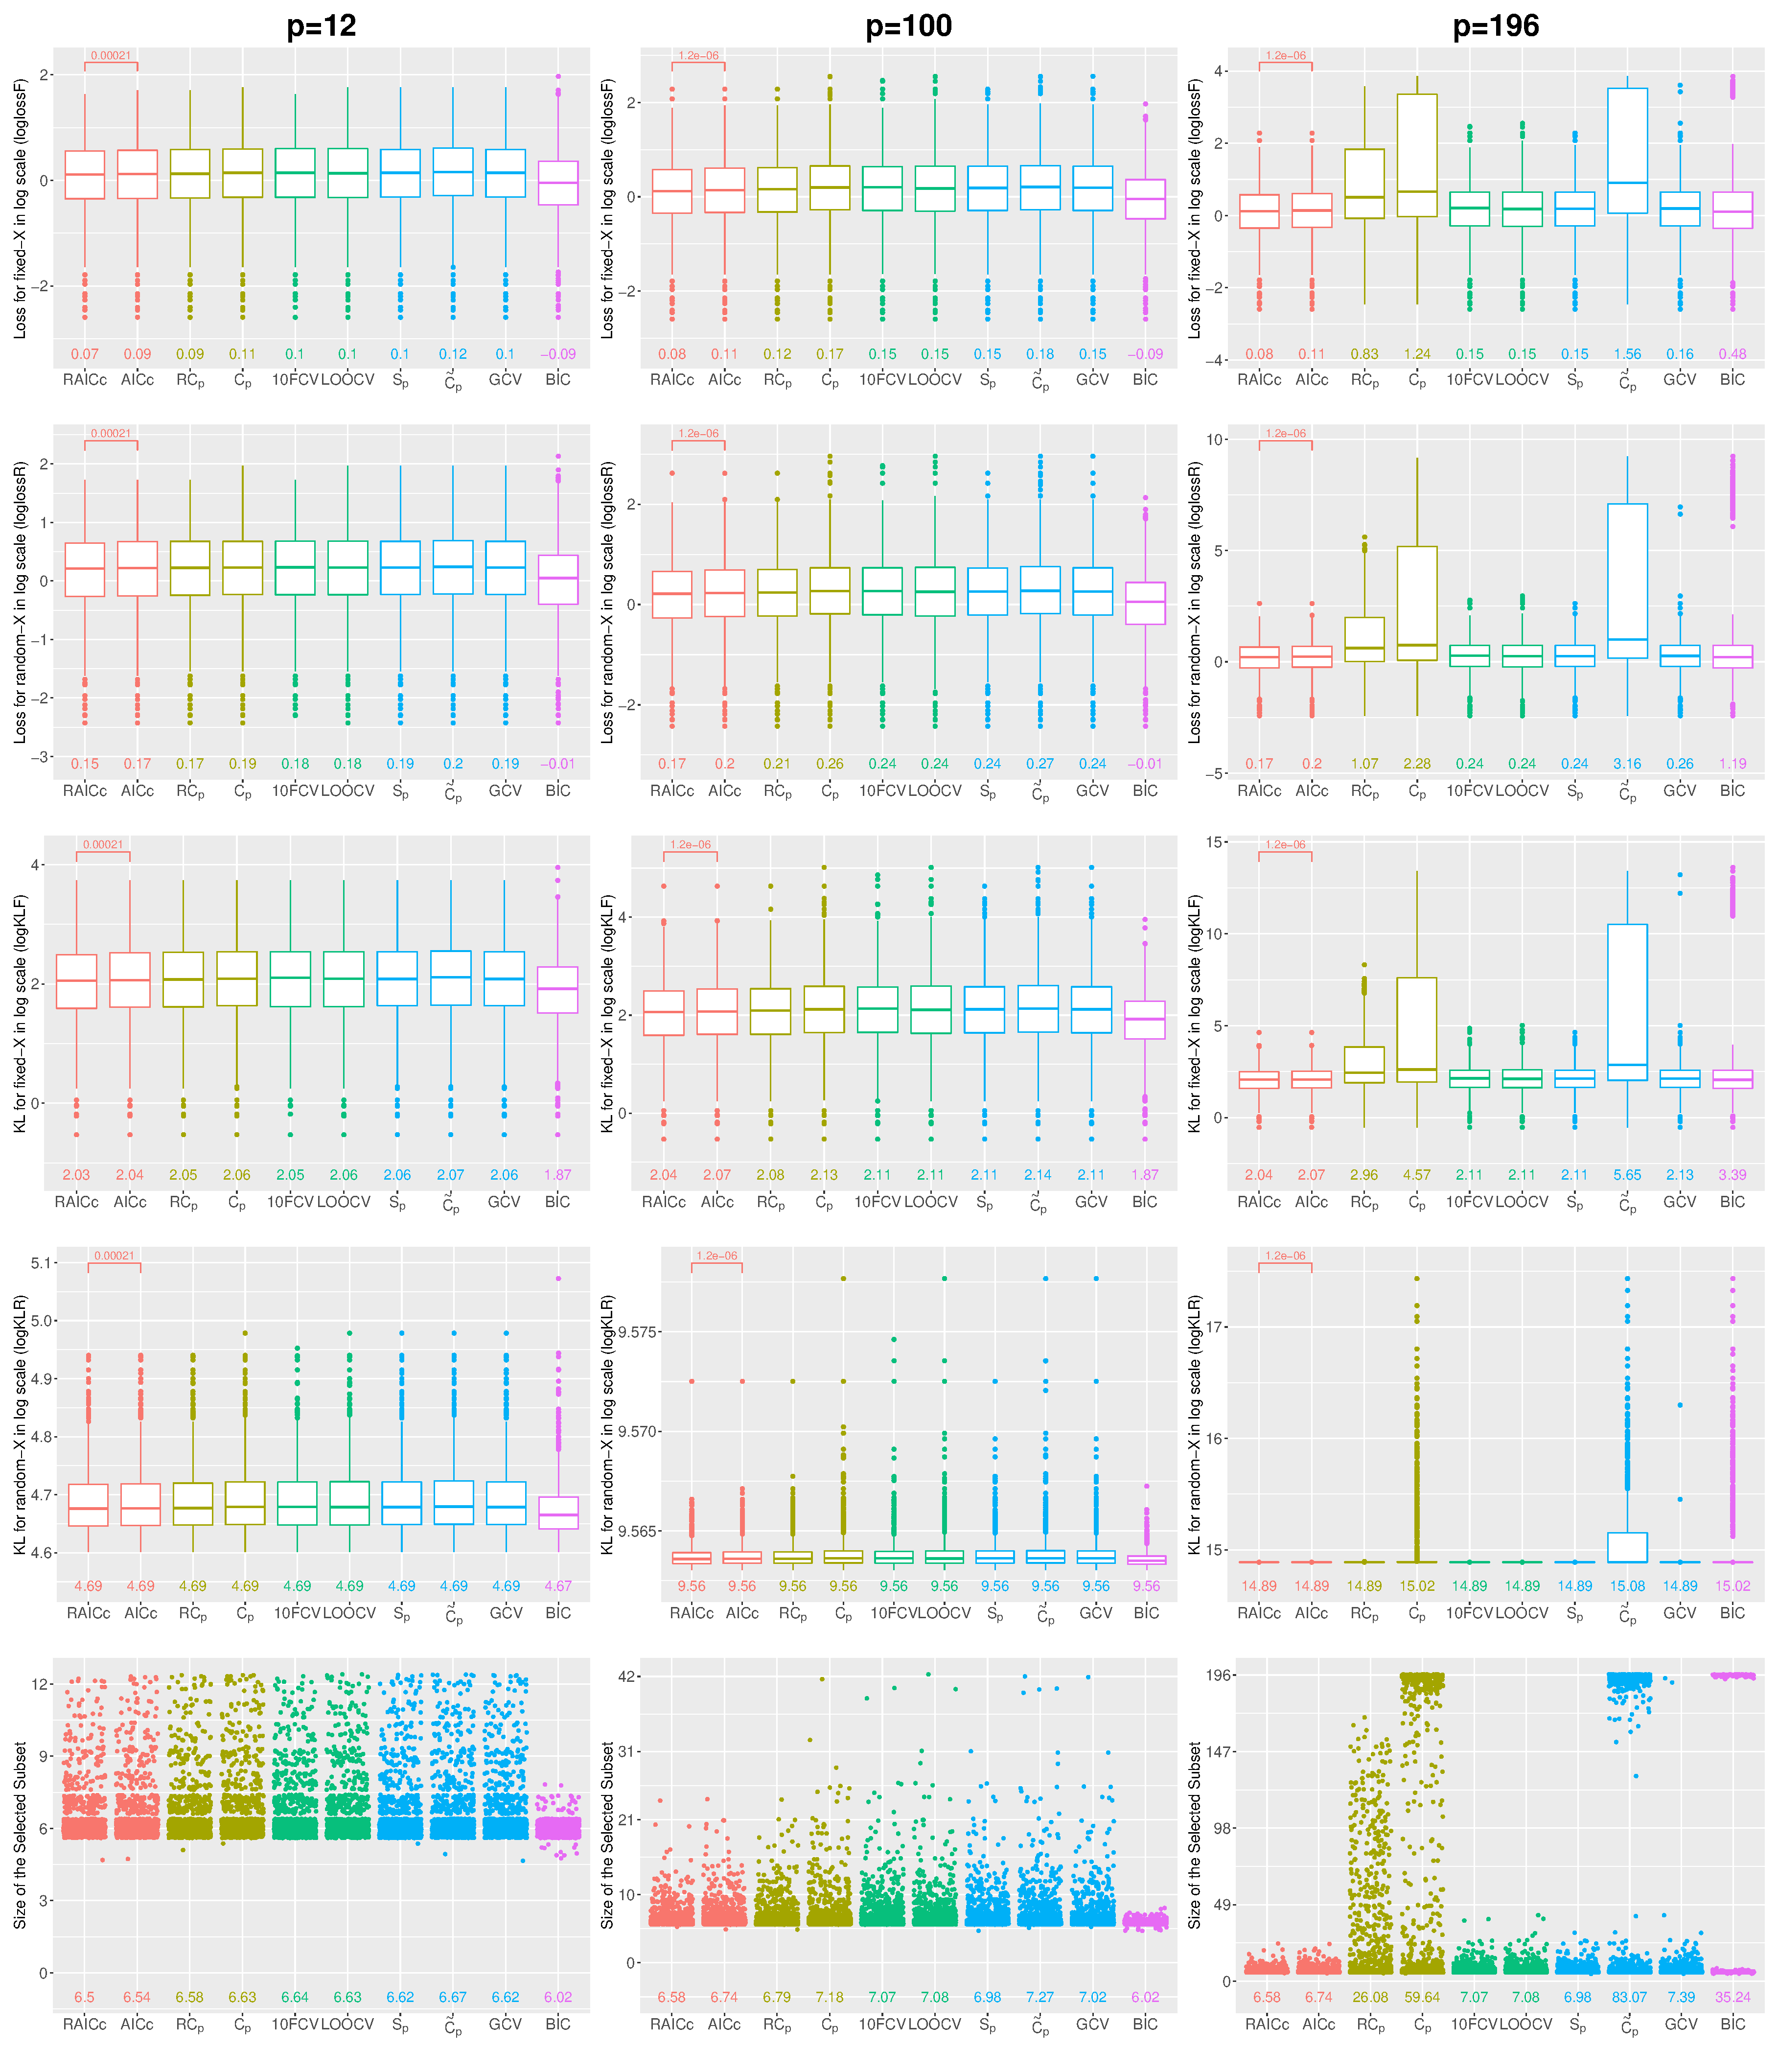
\includegraphics[width=\textwidth]{figures/supplement/fixedx/subset_selection/Sparse-Ex2_n200_hsnr_rho09.eps}
\caption{Variable selection, Fixed-X, Sparse-Ex2, $n=200$, high signal, and $\rho=0.9$.}
\end{figure}
\clearpage
\begin{figure}[!ht]
\centering
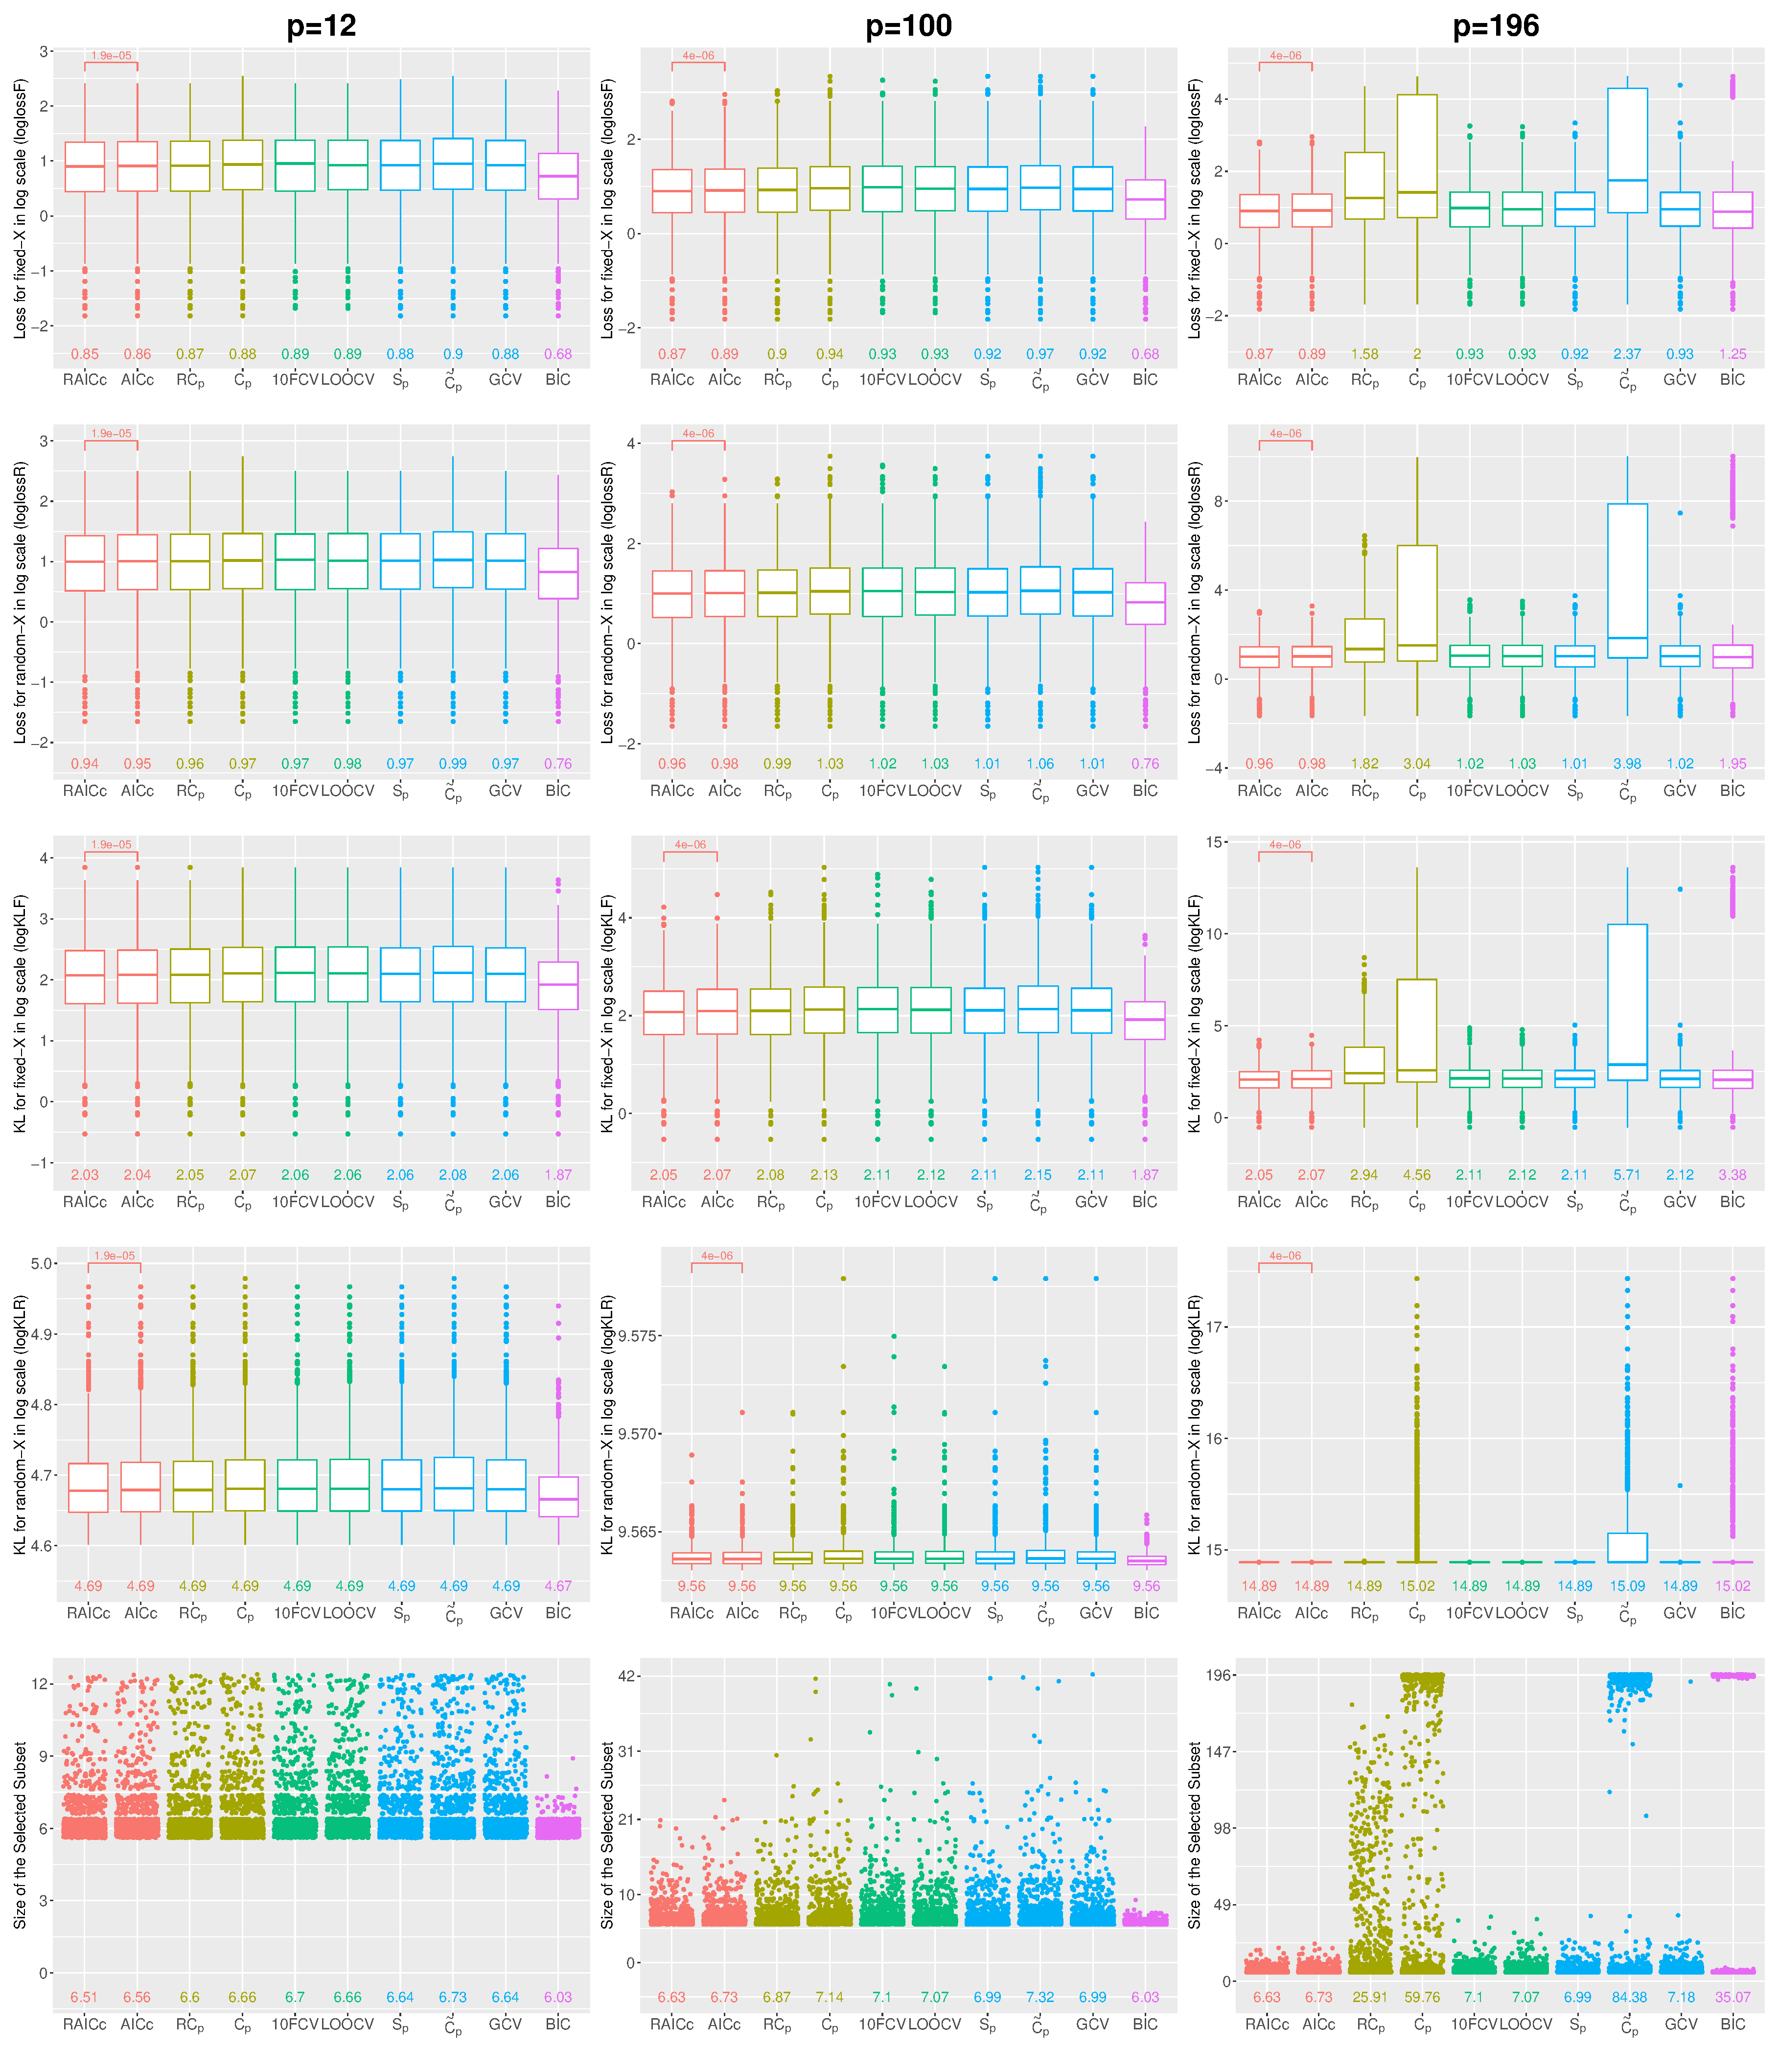
\includegraphics[width=\textwidth]{figures/supplement/fixedx/subset_selection/Sparse-Ex2_n200_msnr_rho0.eps}
\caption{Variable selection, Fixed-X, Sparse-Ex2, $n=200$, medium signal, and $\rho=0$.}
\end{figure}
\clearpage
\begin{figure}[!ht]
\centering
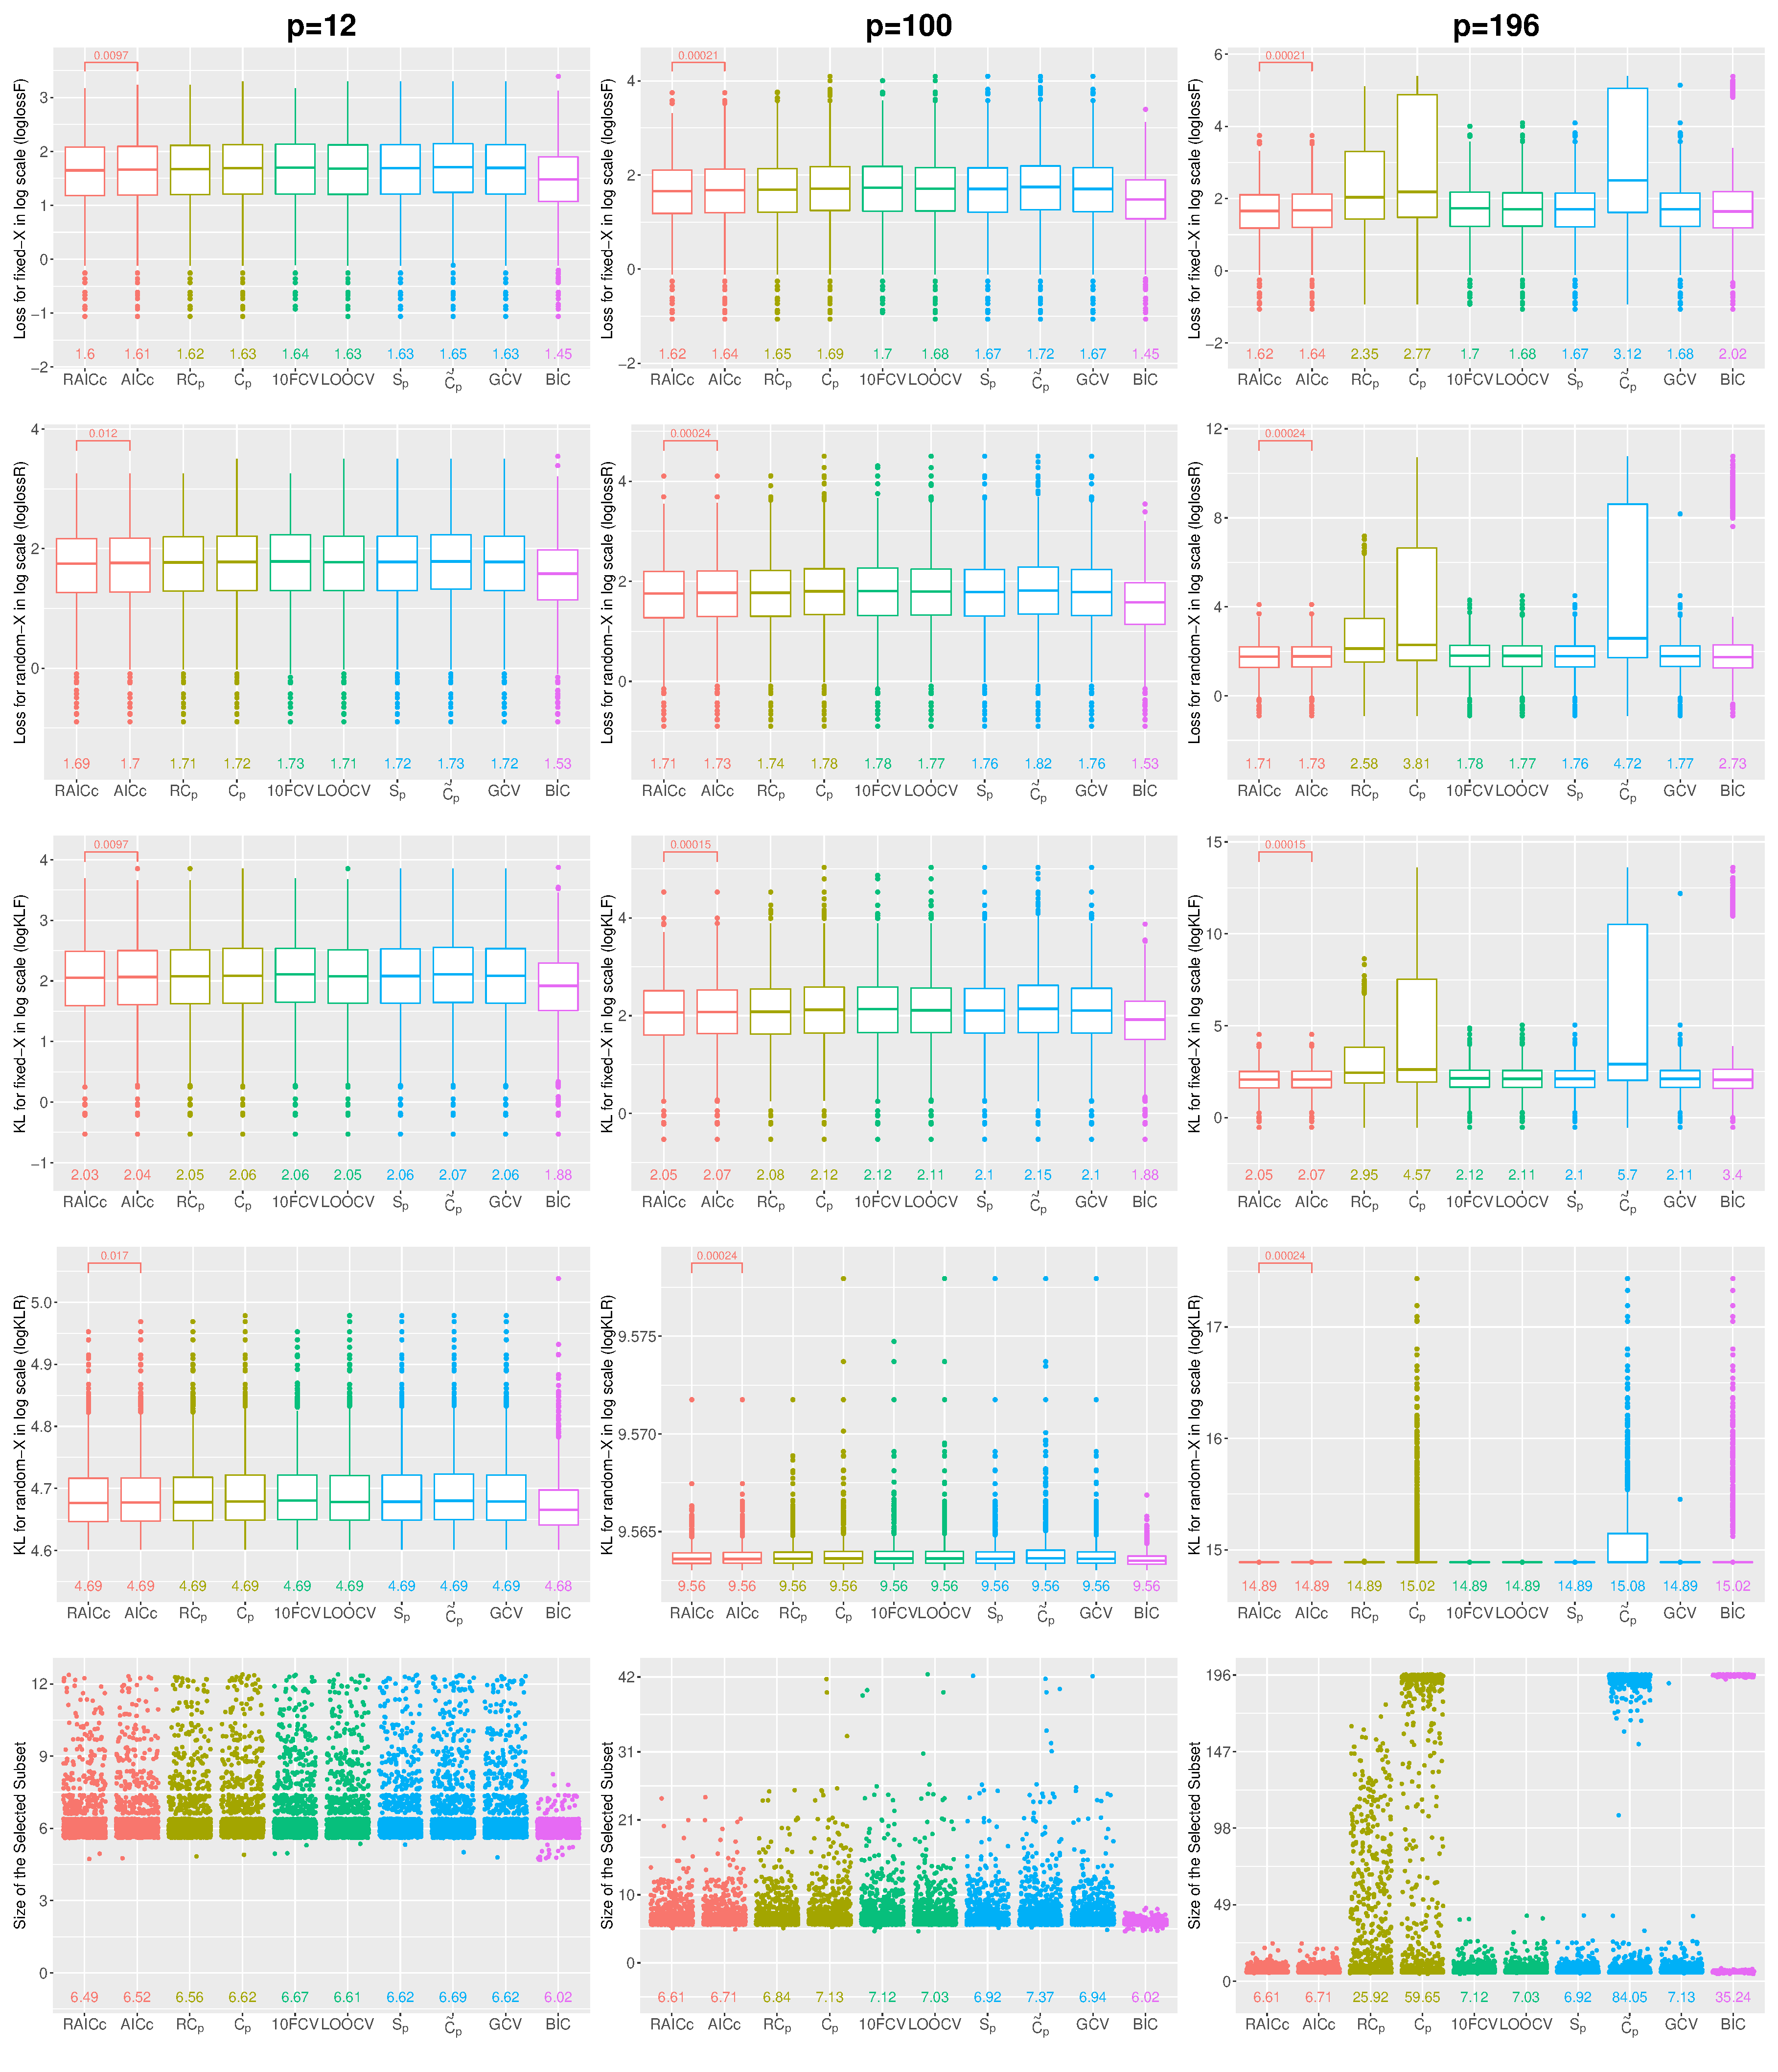
\includegraphics[width=\textwidth]{figures/supplement/fixedx/subset_selection/Sparse-Ex2_n200_msnr_rho05.eps}
\caption{Variable selection, Fixed-X, Sparse-Ex2, $n=200$, medium signal, and $\rho=0.5$.}
\end{figure}
\clearpage
\begin{figure}[!ht]
\centering
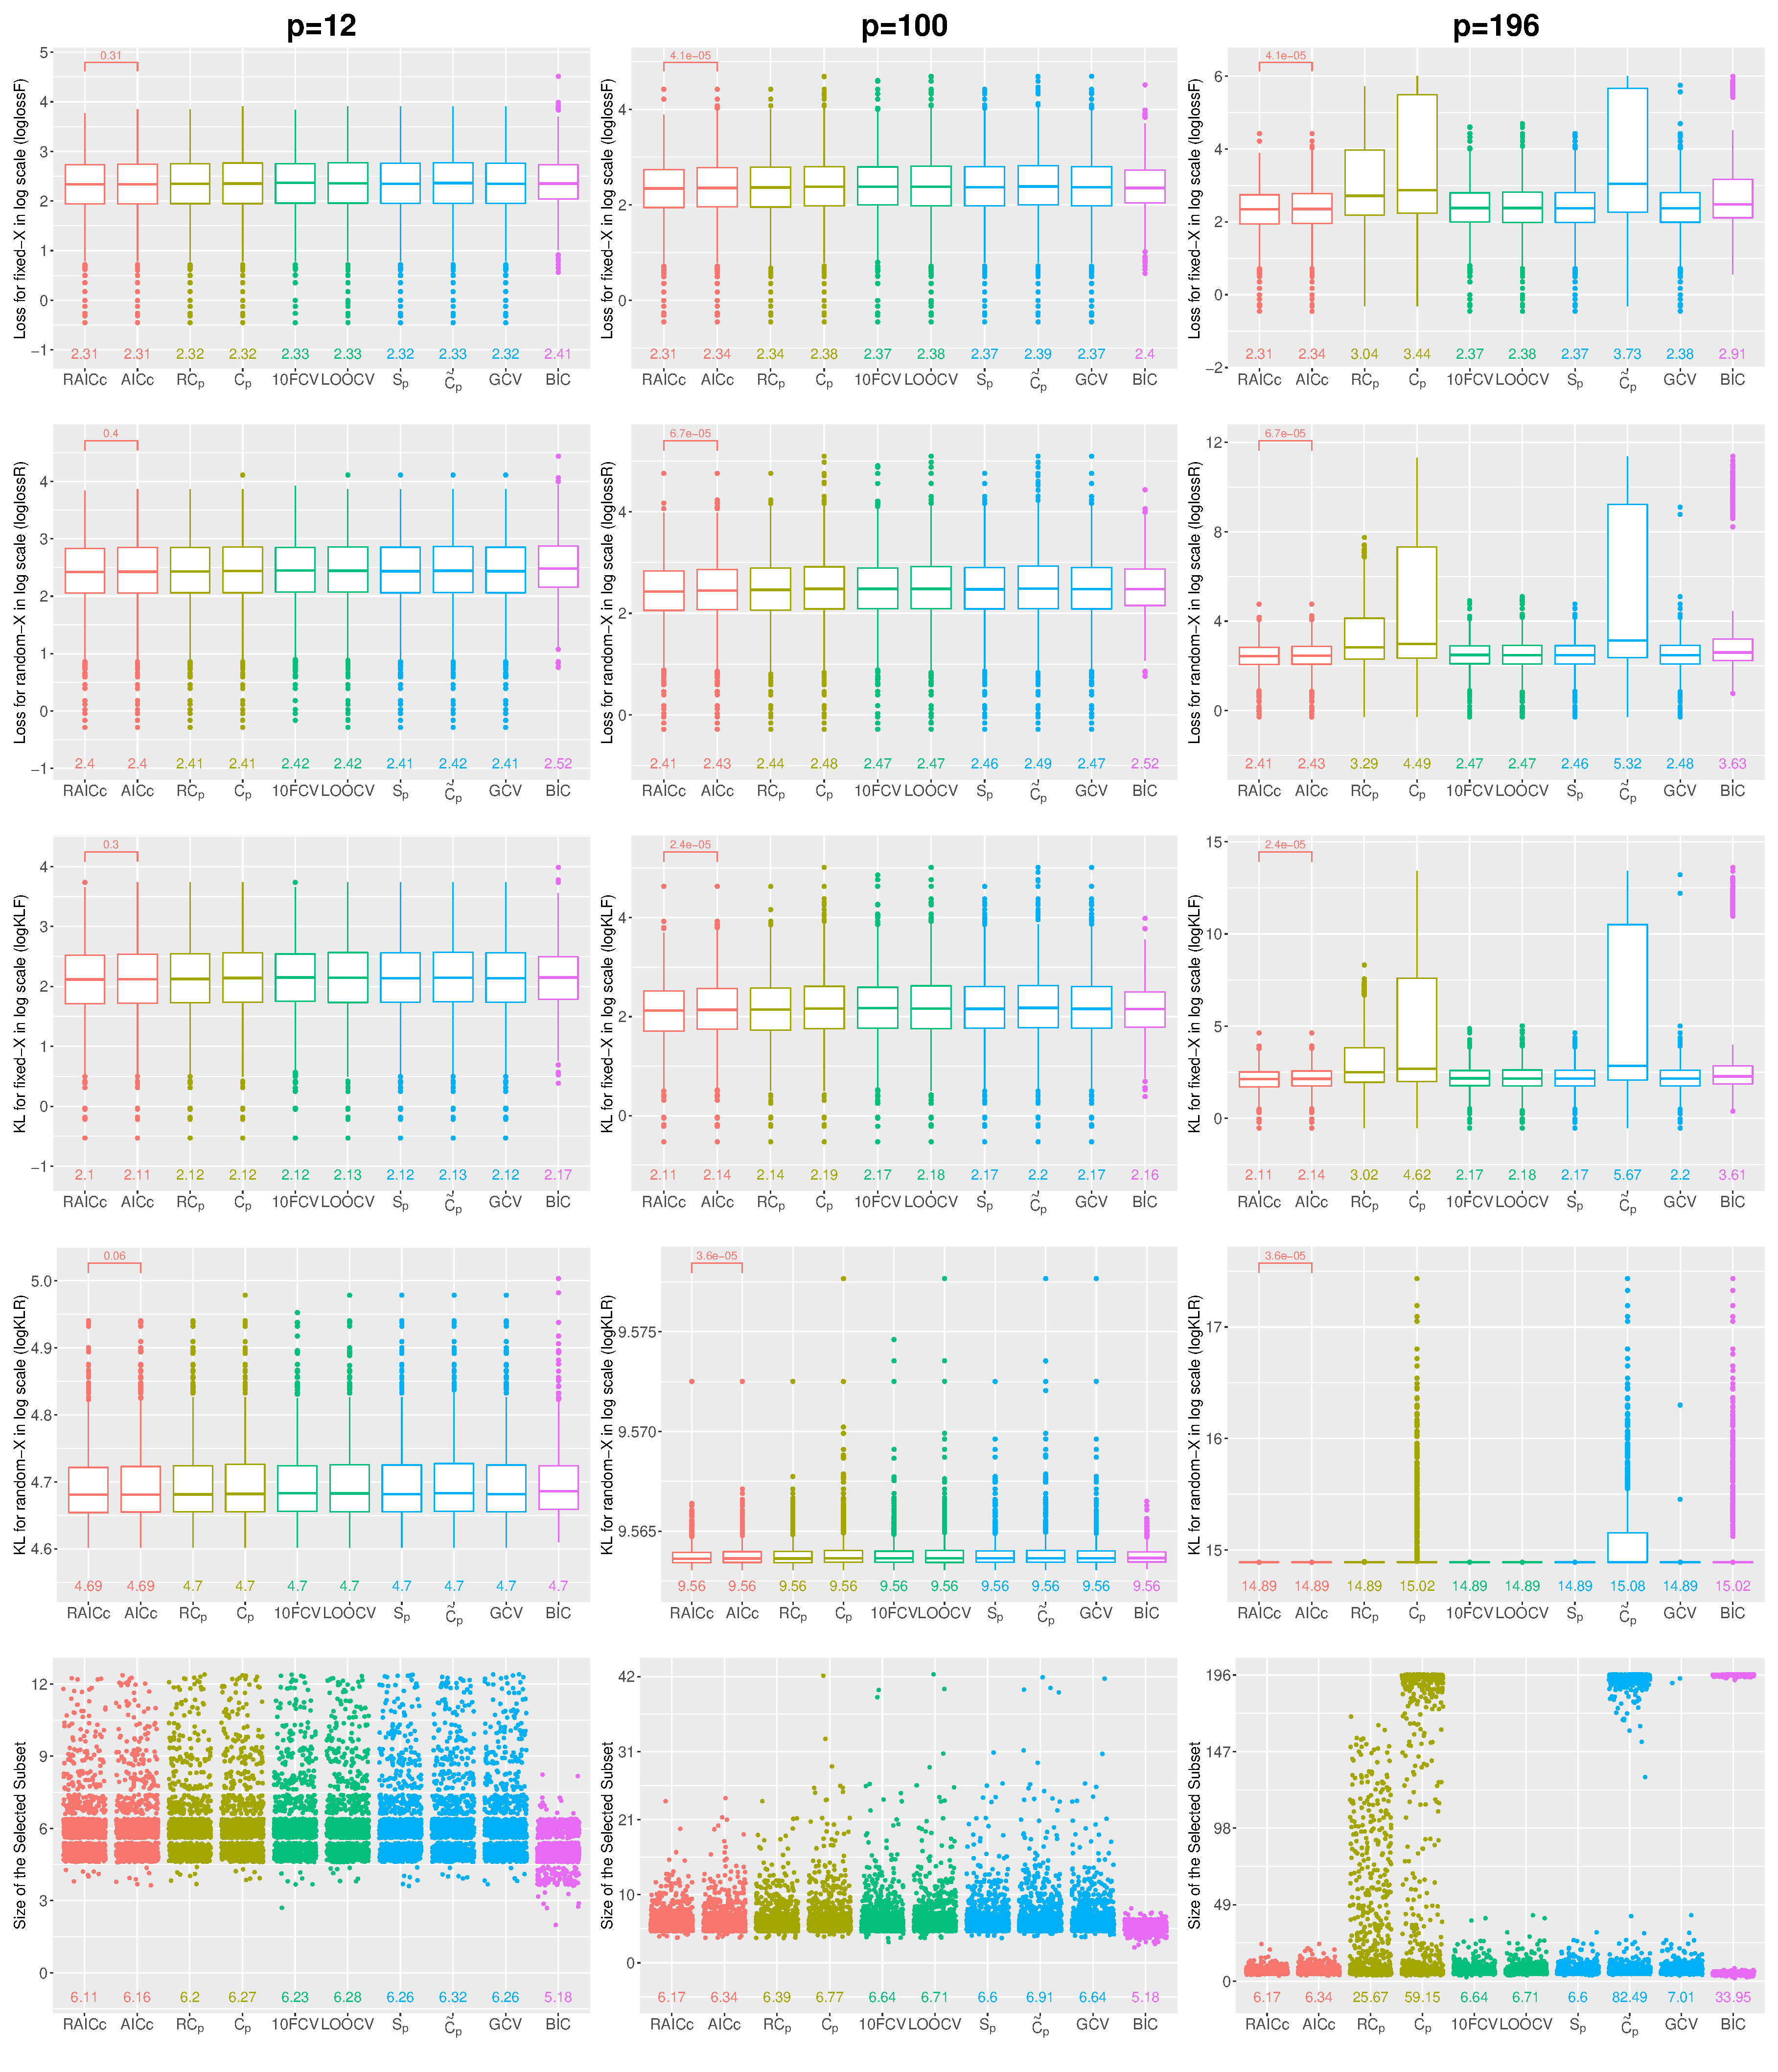
\includegraphics[width=\textwidth]{figures/supplement/fixedx/subset_selection/Sparse-Ex2_n200_msnr_rho09.eps}
\caption{Variable selection, Fixed-X, Sparse-Ex2, $n=200$, medium signal, and $\rho=0.9$.}
\end{figure}
\clearpage
\begin{figure}[!ht]
\centering
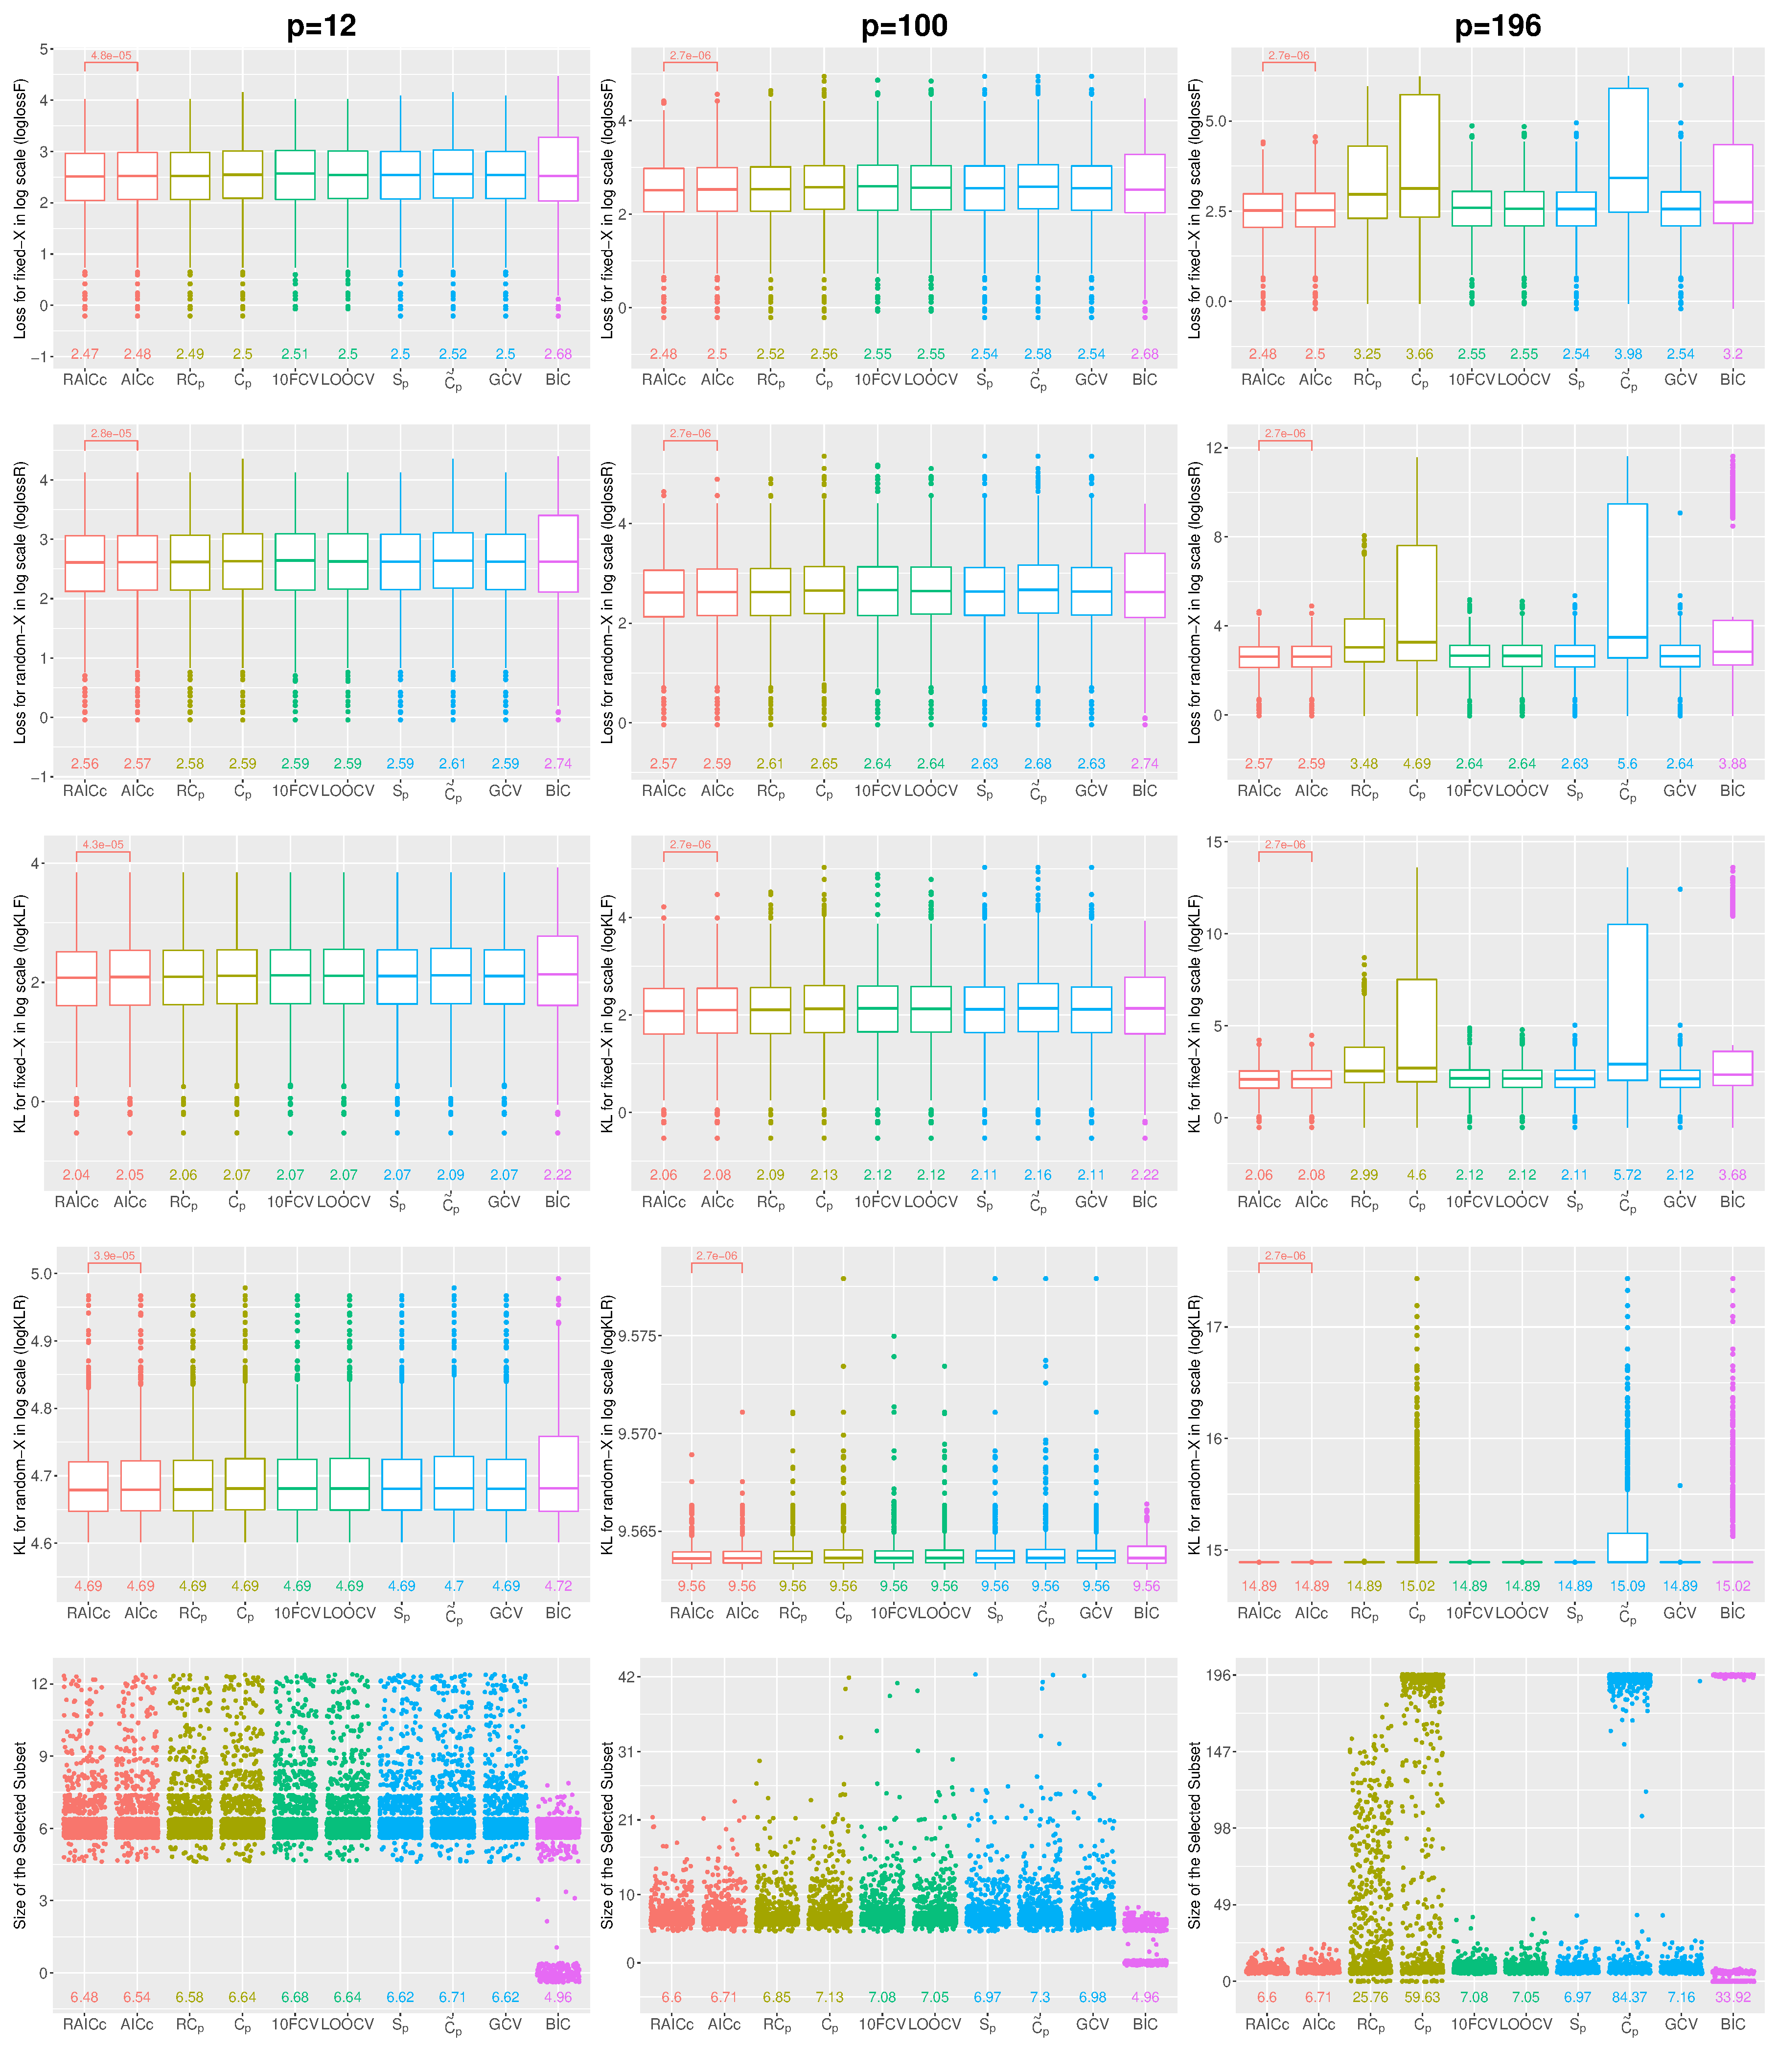
\includegraphics[width=\textwidth]{figures/supplement/fixedx/subset_selection/Sparse-Ex2_n200_lsnr_rho0.eps}
\caption{Variable selection, Fixed-X, Sparse-Ex2, $n=200$, low signal, and $\rho=0$.}
\end{figure}
\clearpage
\begin{figure}[!ht]
\centering
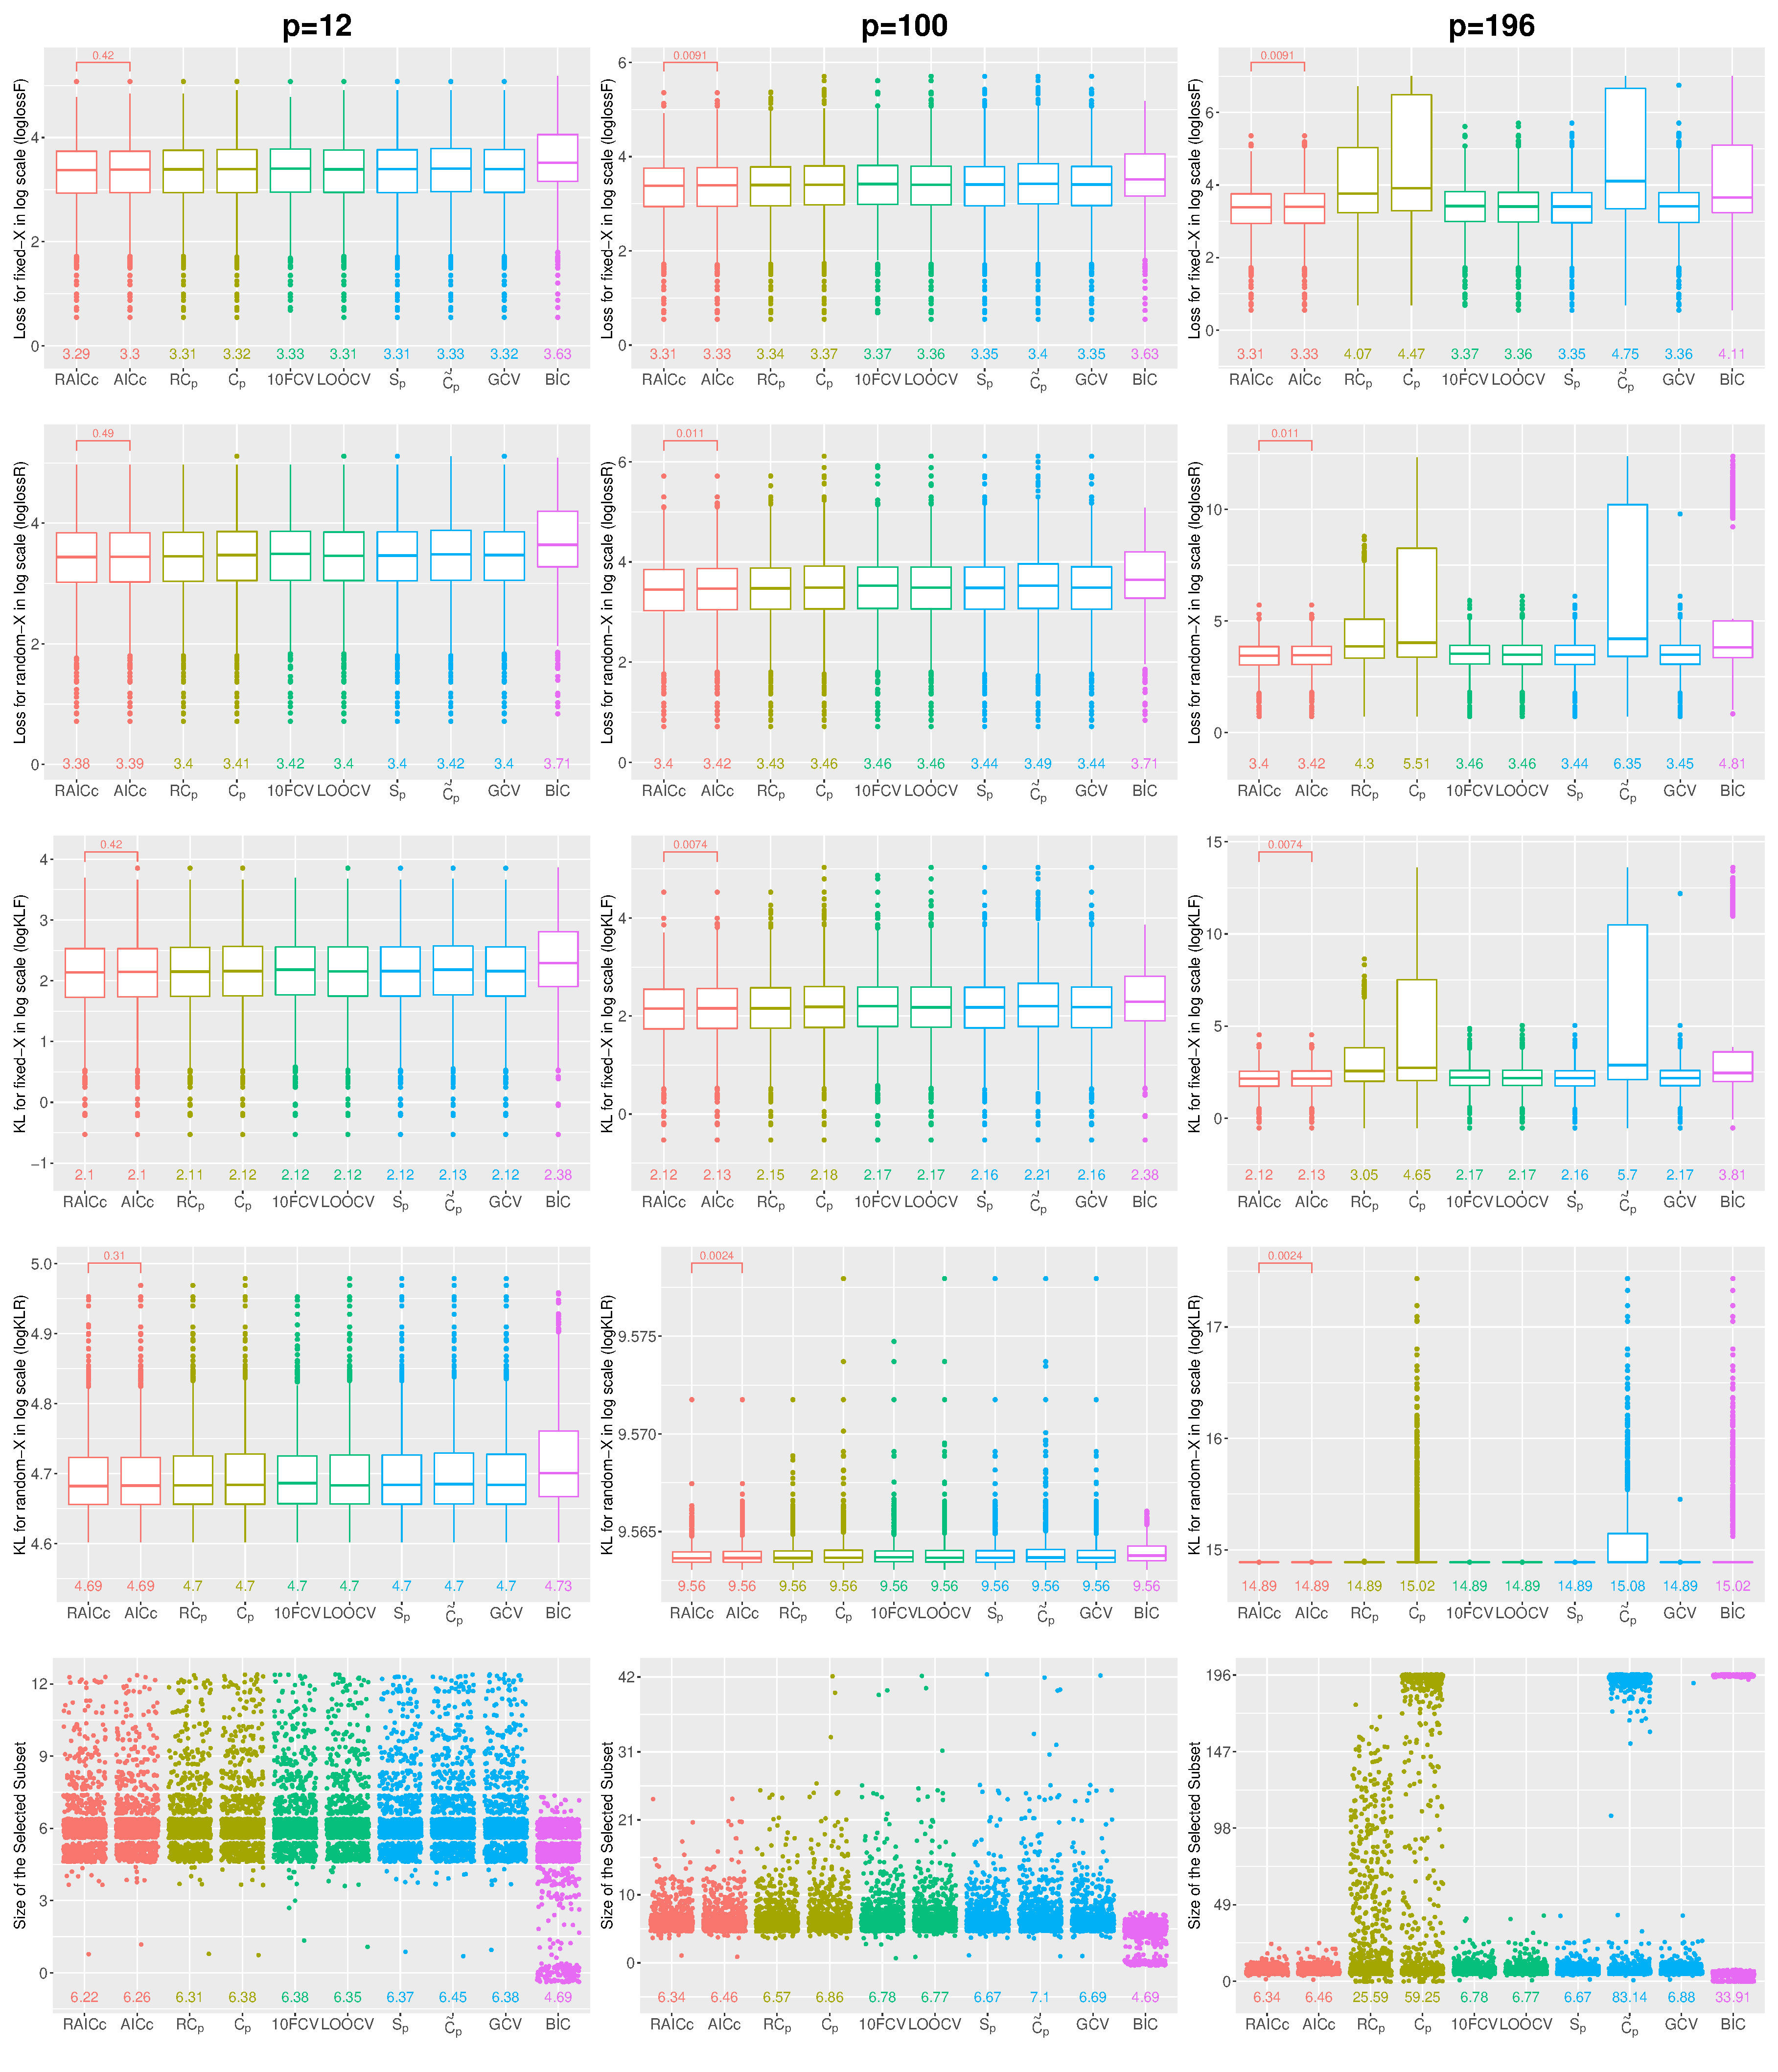
\includegraphics[width=\textwidth]{figures/supplement/fixedx/subset_selection/Sparse-Ex2_n200_lsnr_rho05.eps}
\caption{Variable selection, Fixed-X, Sparse-Ex2, $n=200$, low signal, and $\rho=0.5$.}
\end{figure}
\clearpage
\begin{figure}[!ht]
\centering
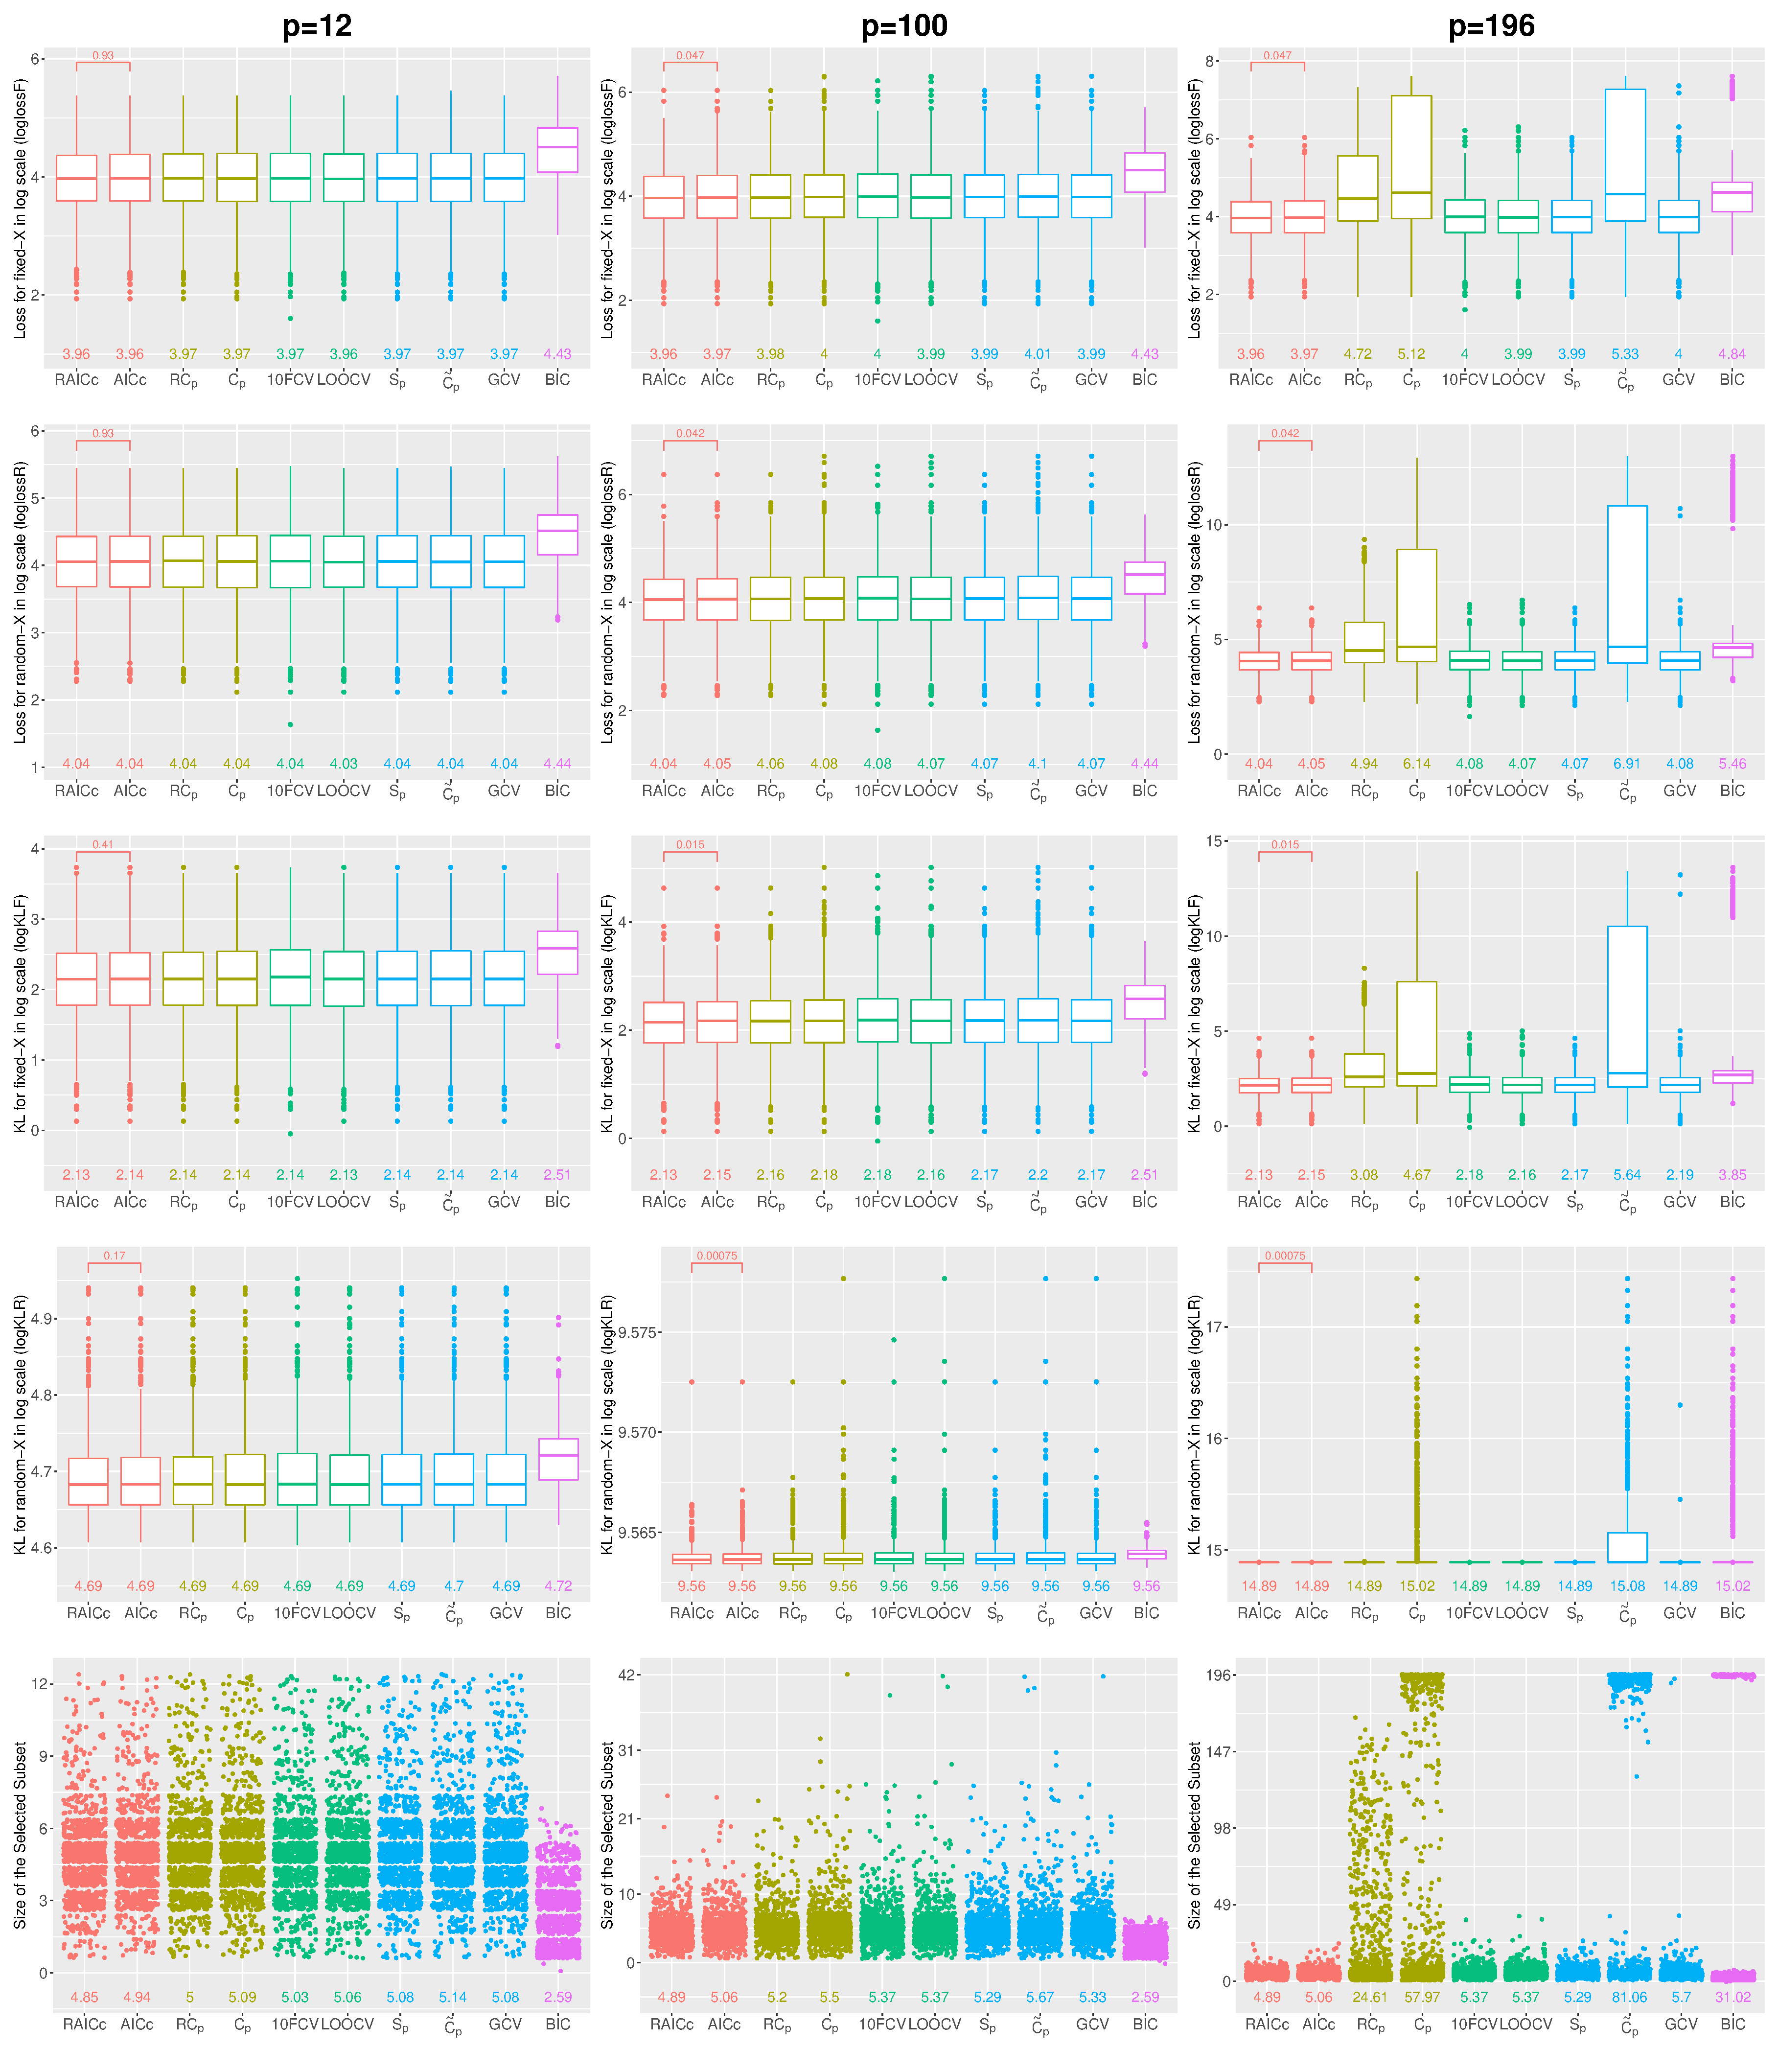
\includegraphics[width=\textwidth]{figures/supplement/fixedx/subset_selection/Sparse-Ex2_n200_lsnr_rho09.eps}
\caption{Variable selection, Fixed-X, Sparse-Ex2, $n=200$, low signal, and $\rho=0.9$.}
\end{figure}
\clearpage
\begin{figure}[!ht]
\centering
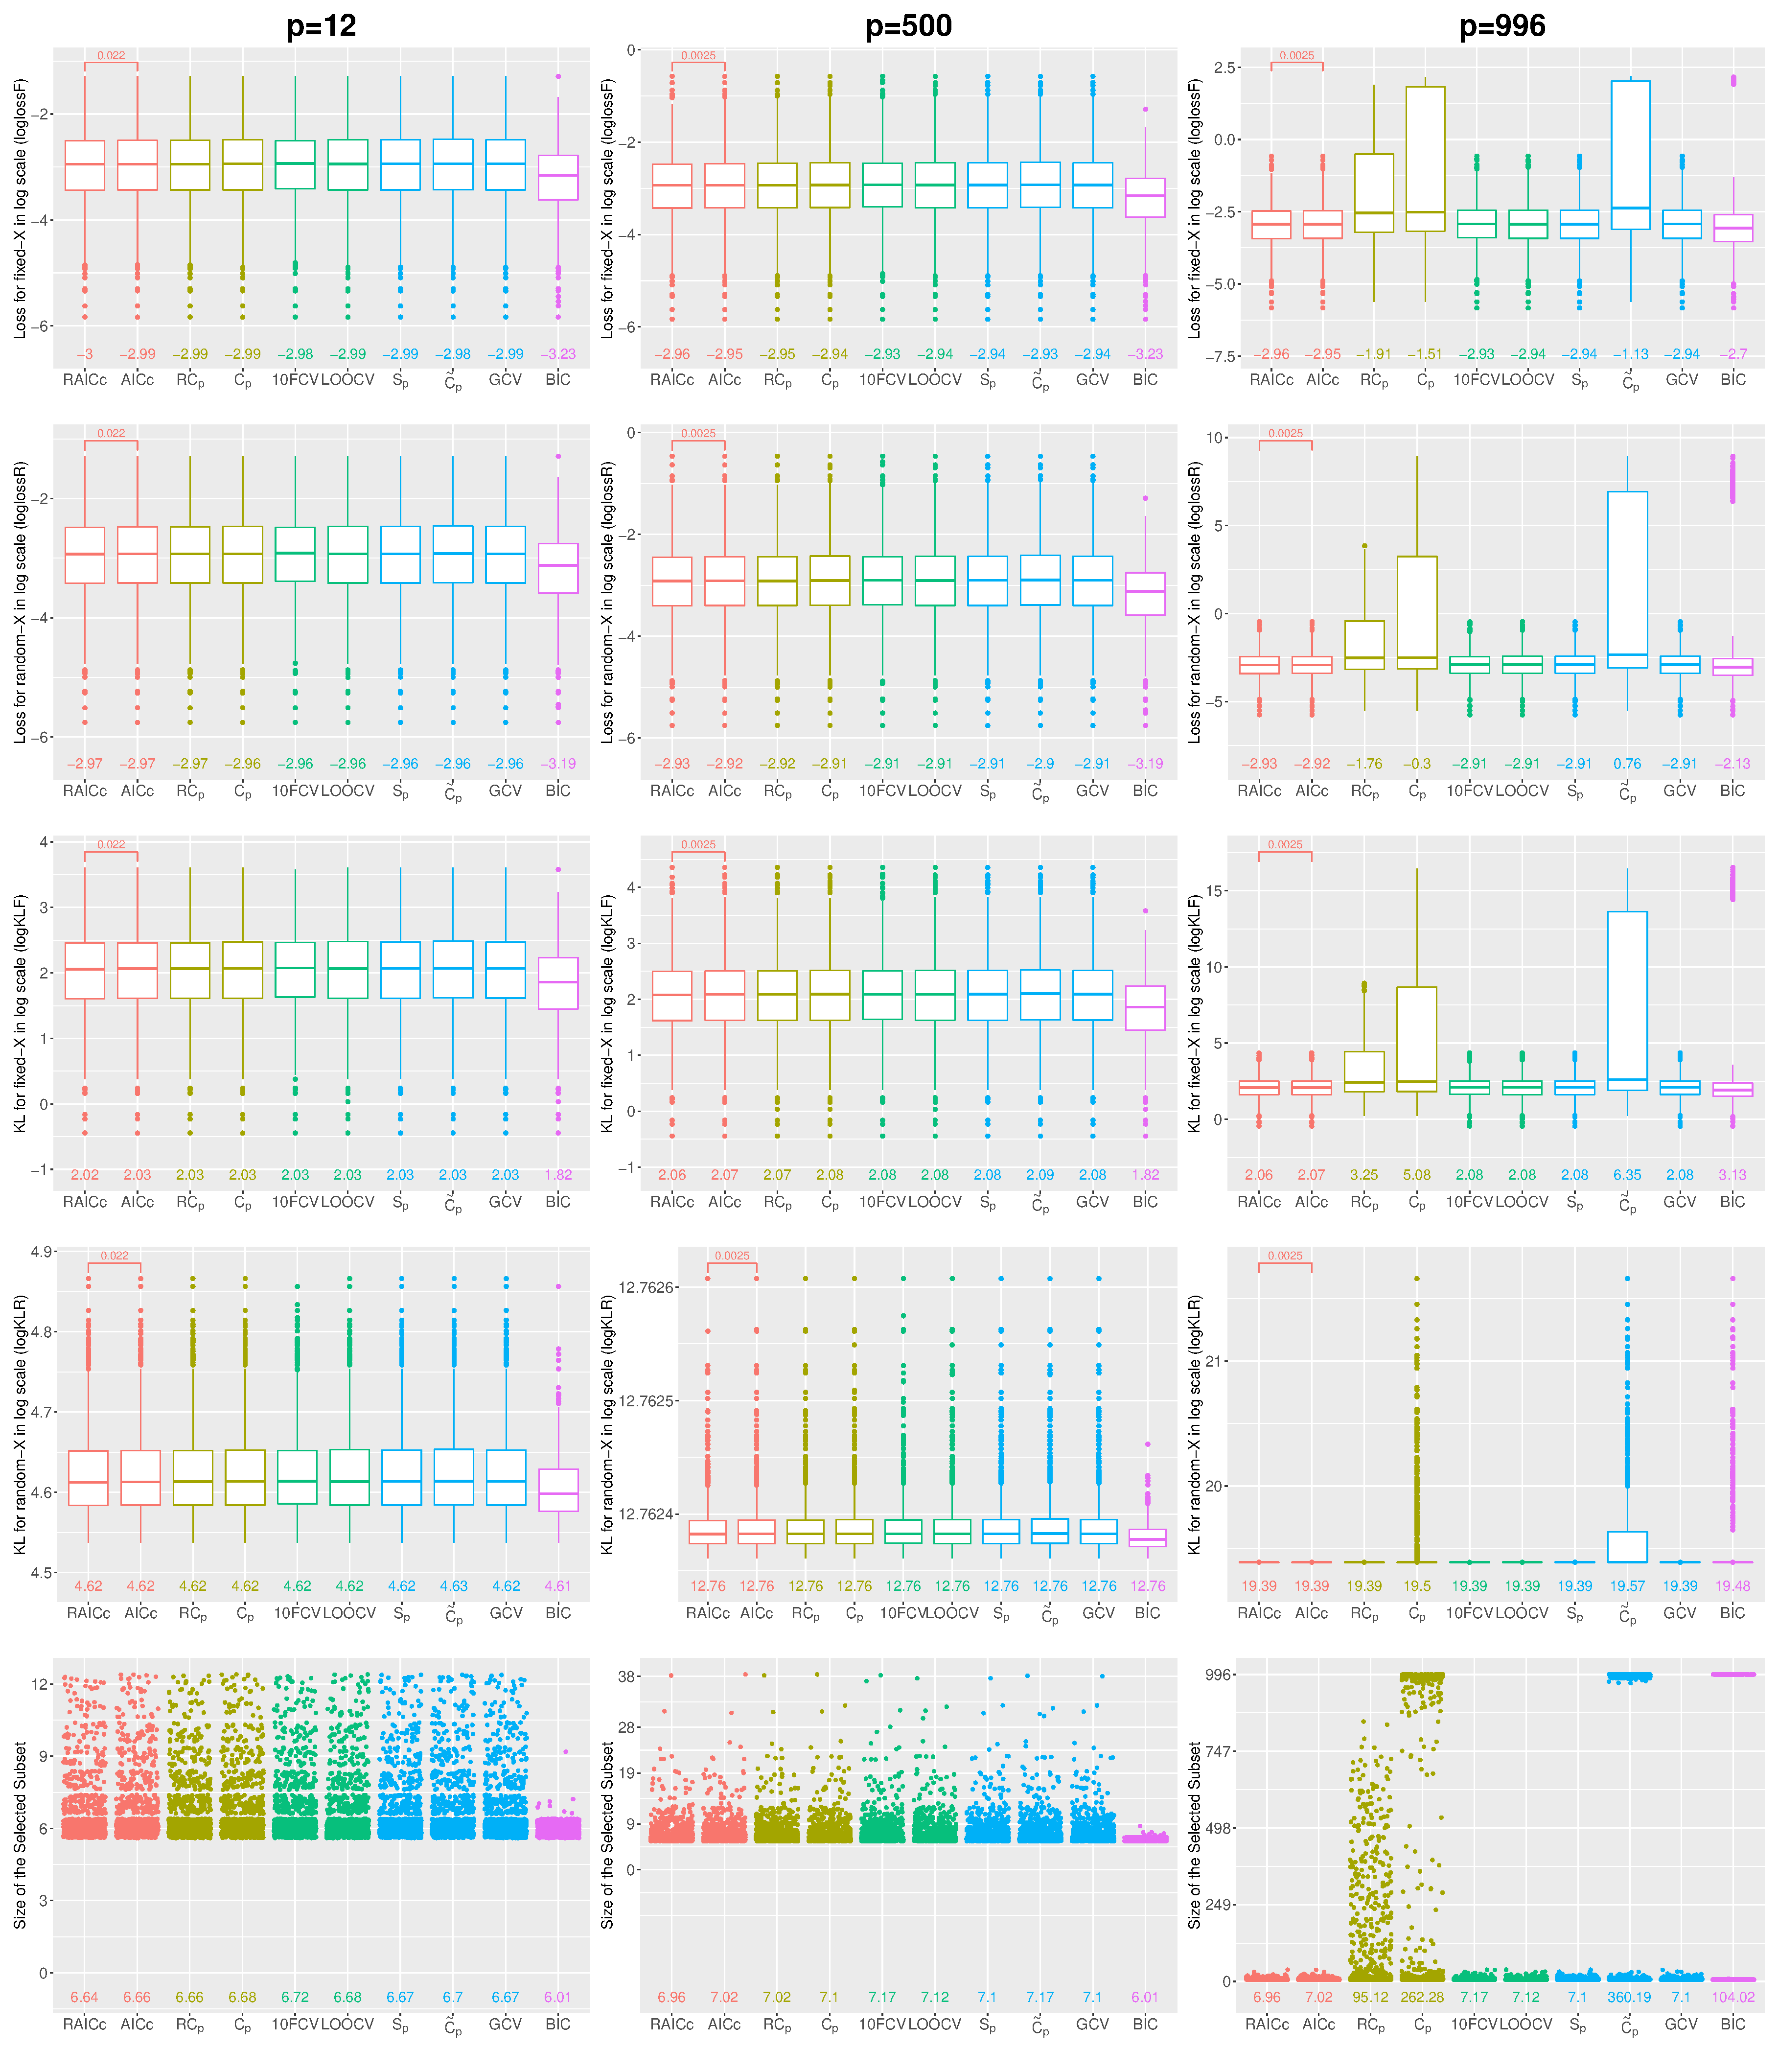
\includegraphics[width=\textwidth]{figures/supplement/fixedx/subset_selection/Sparse-Ex2_n1000_hsnr_rho0.eps}
\caption{Variable selection, Fixed-X, Sparse-Ex2, $n=1000$, high signal, and $\rho=0$.}
\end{figure}
\clearpage
\begin{figure}[!ht]
\centering
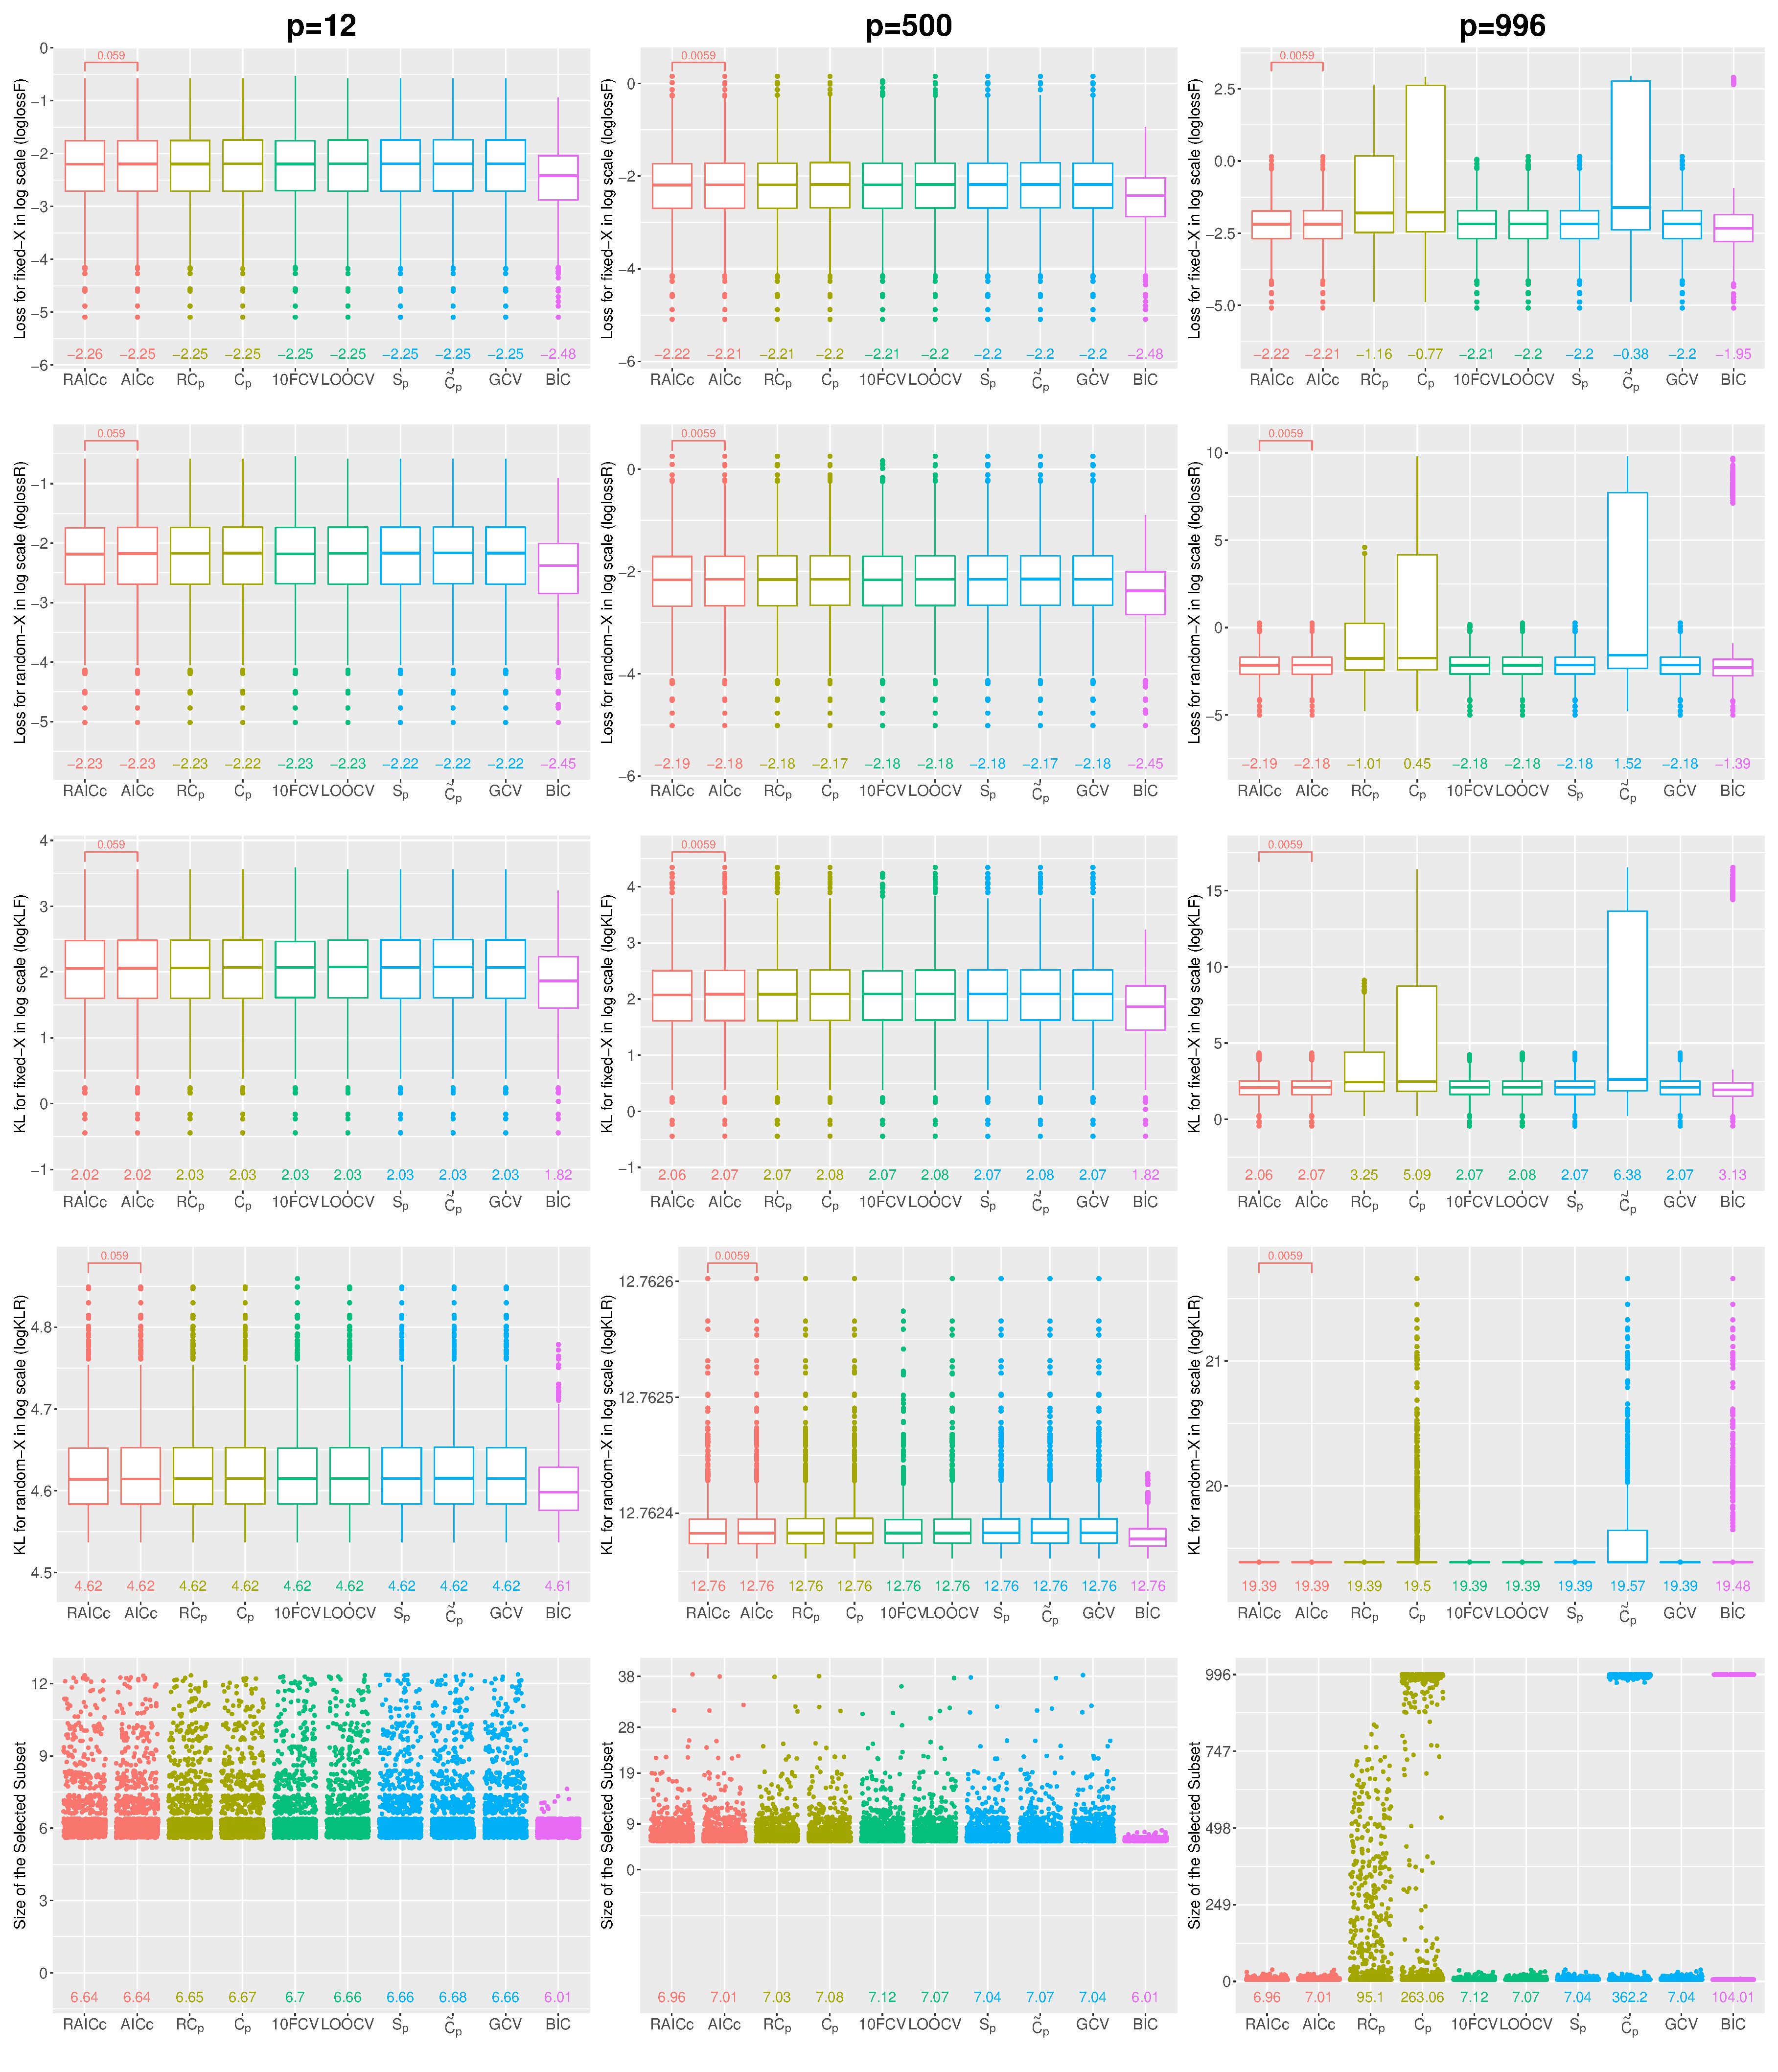
\includegraphics[width=\textwidth]{figures/supplement/fixedx/subset_selection/Sparse-Ex2_n1000_hsnr_rho05.eps}
\caption{Variable selection, Fixed-X, Sparse-Ex2, $n=1000$, high signal, and $\rho=0.5$.}
\end{figure}
\clearpage
\begin{figure}[!ht]
\centering
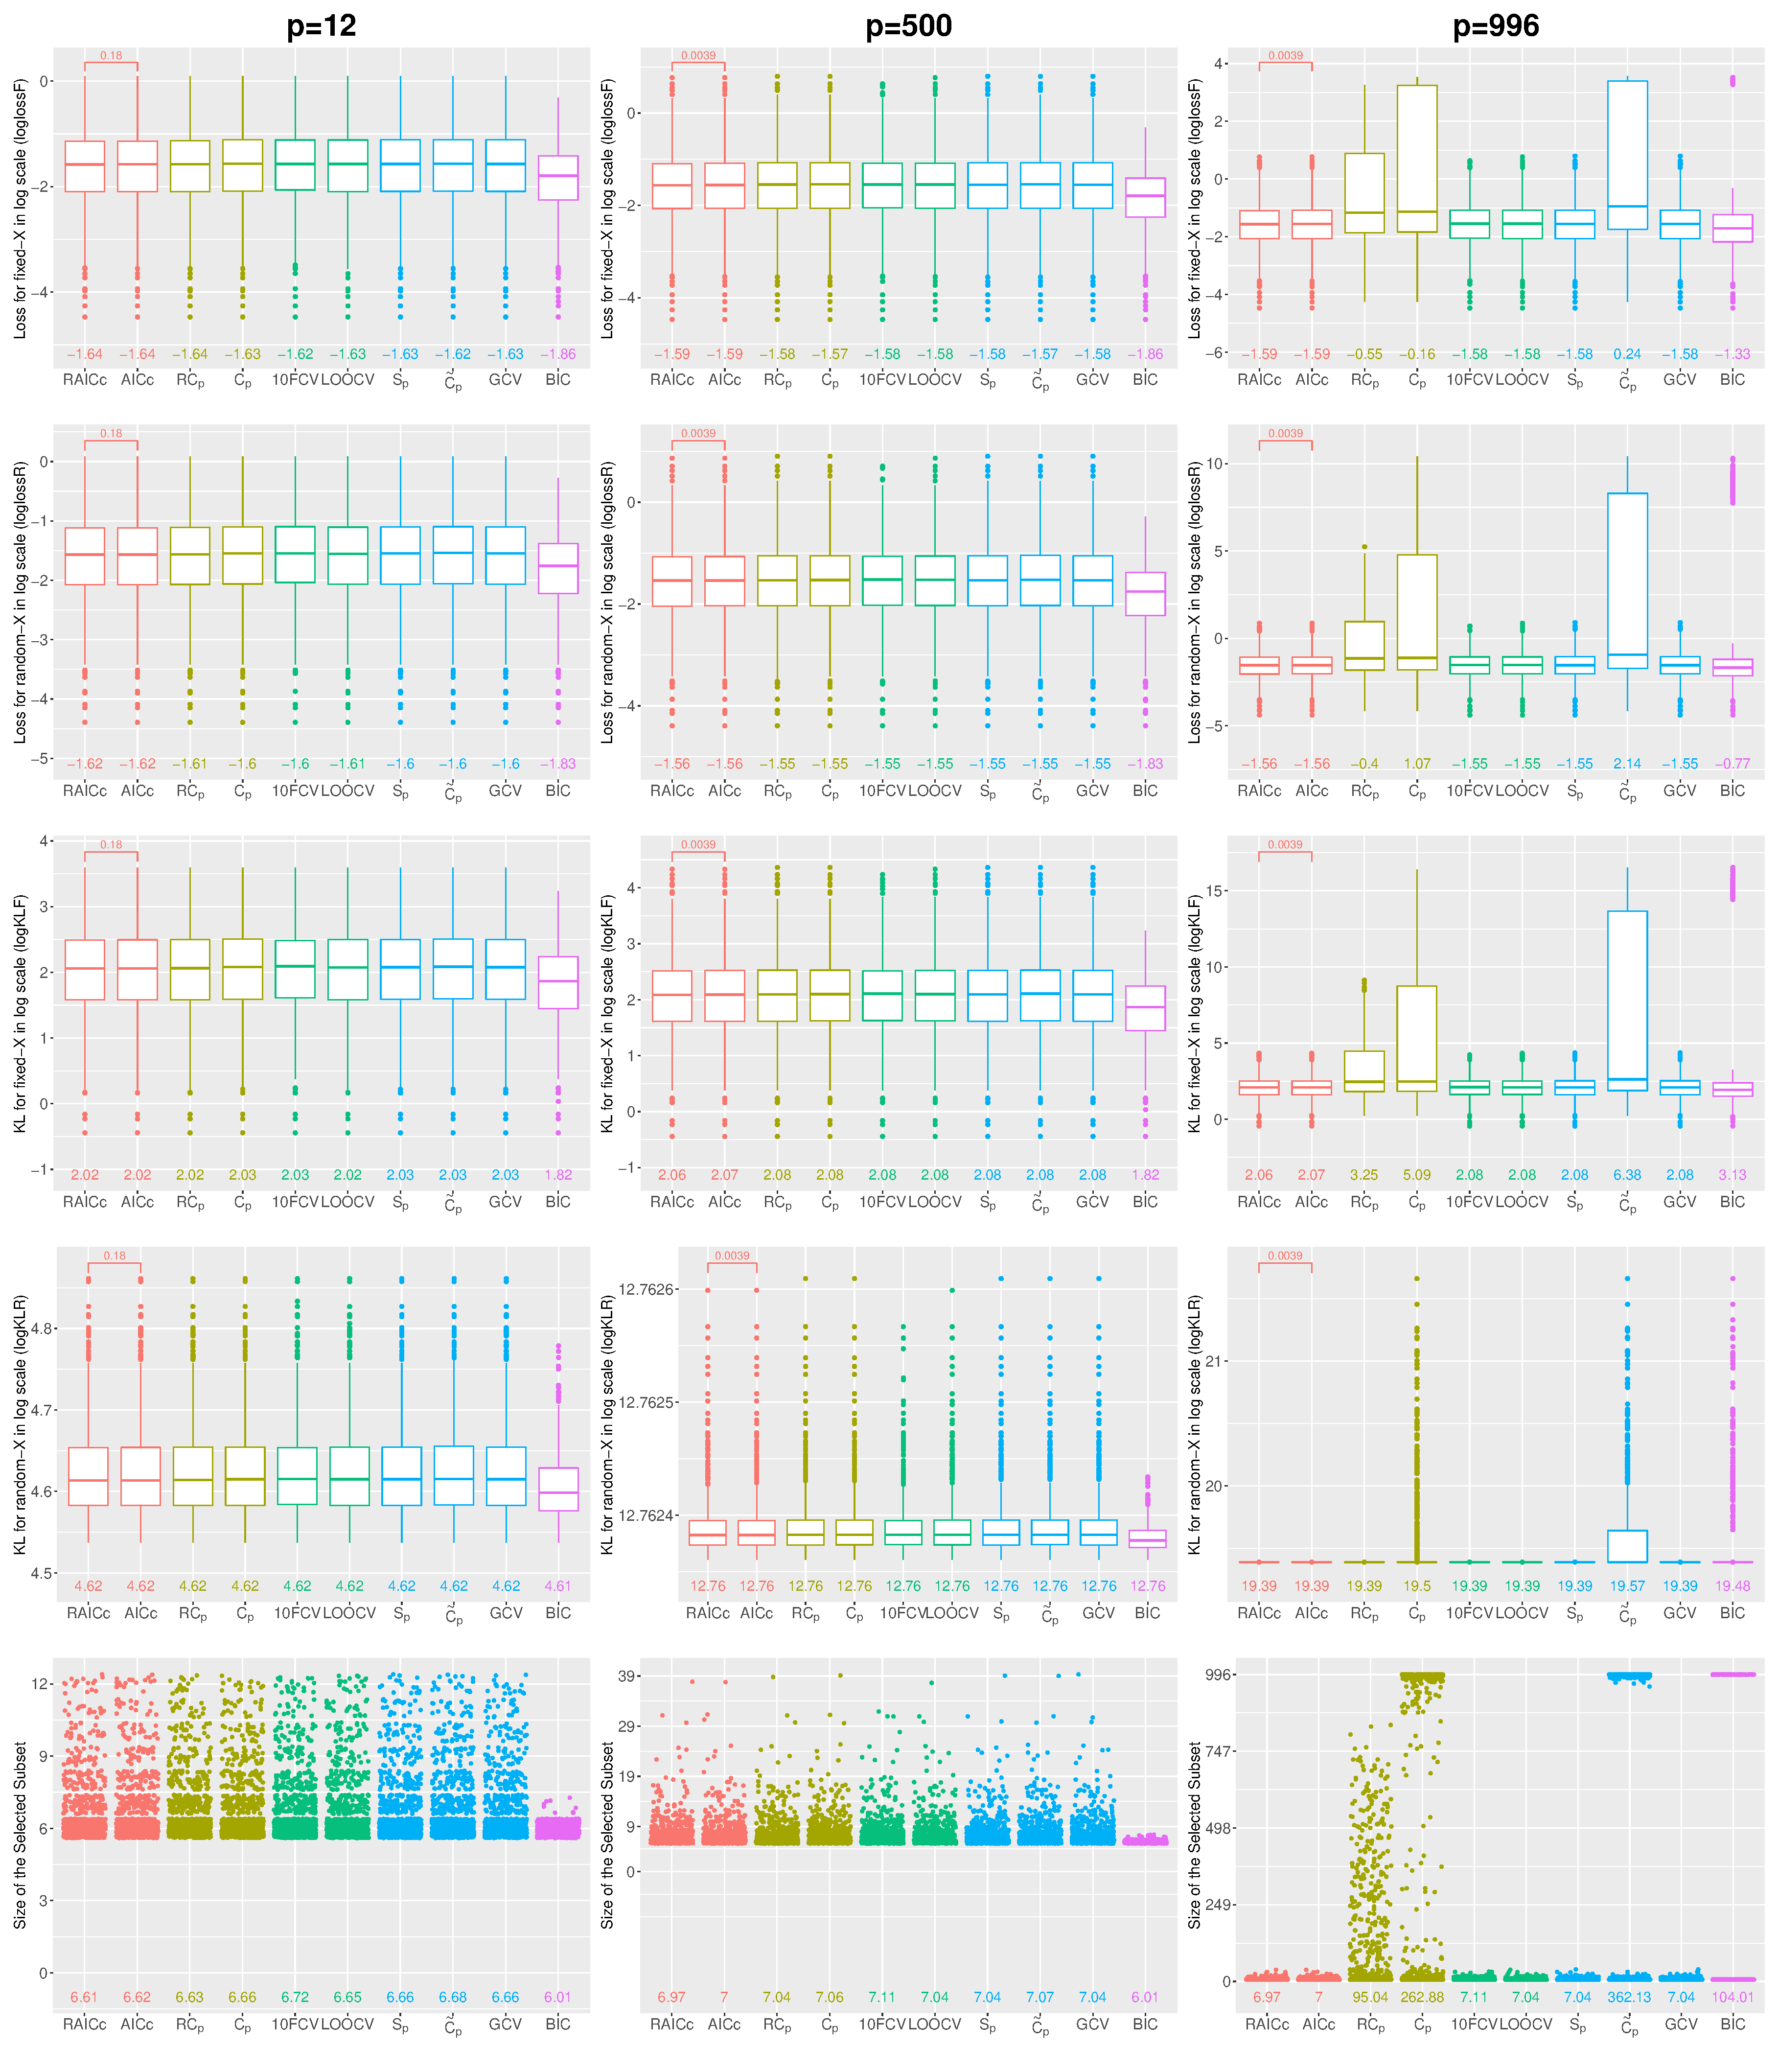
\includegraphics[width=\textwidth]{figures/supplement/fixedx/subset_selection/Sparse-Ex2_n1000_hsnr_rho09.eps}
\caption{Variable selection, Fixed-X, Sparse-Ex2, $n=1000$, high signal, and $\rho=0.9$.}
\end{figure}
\clearpage
\begin{figure}[!ht]
\centering
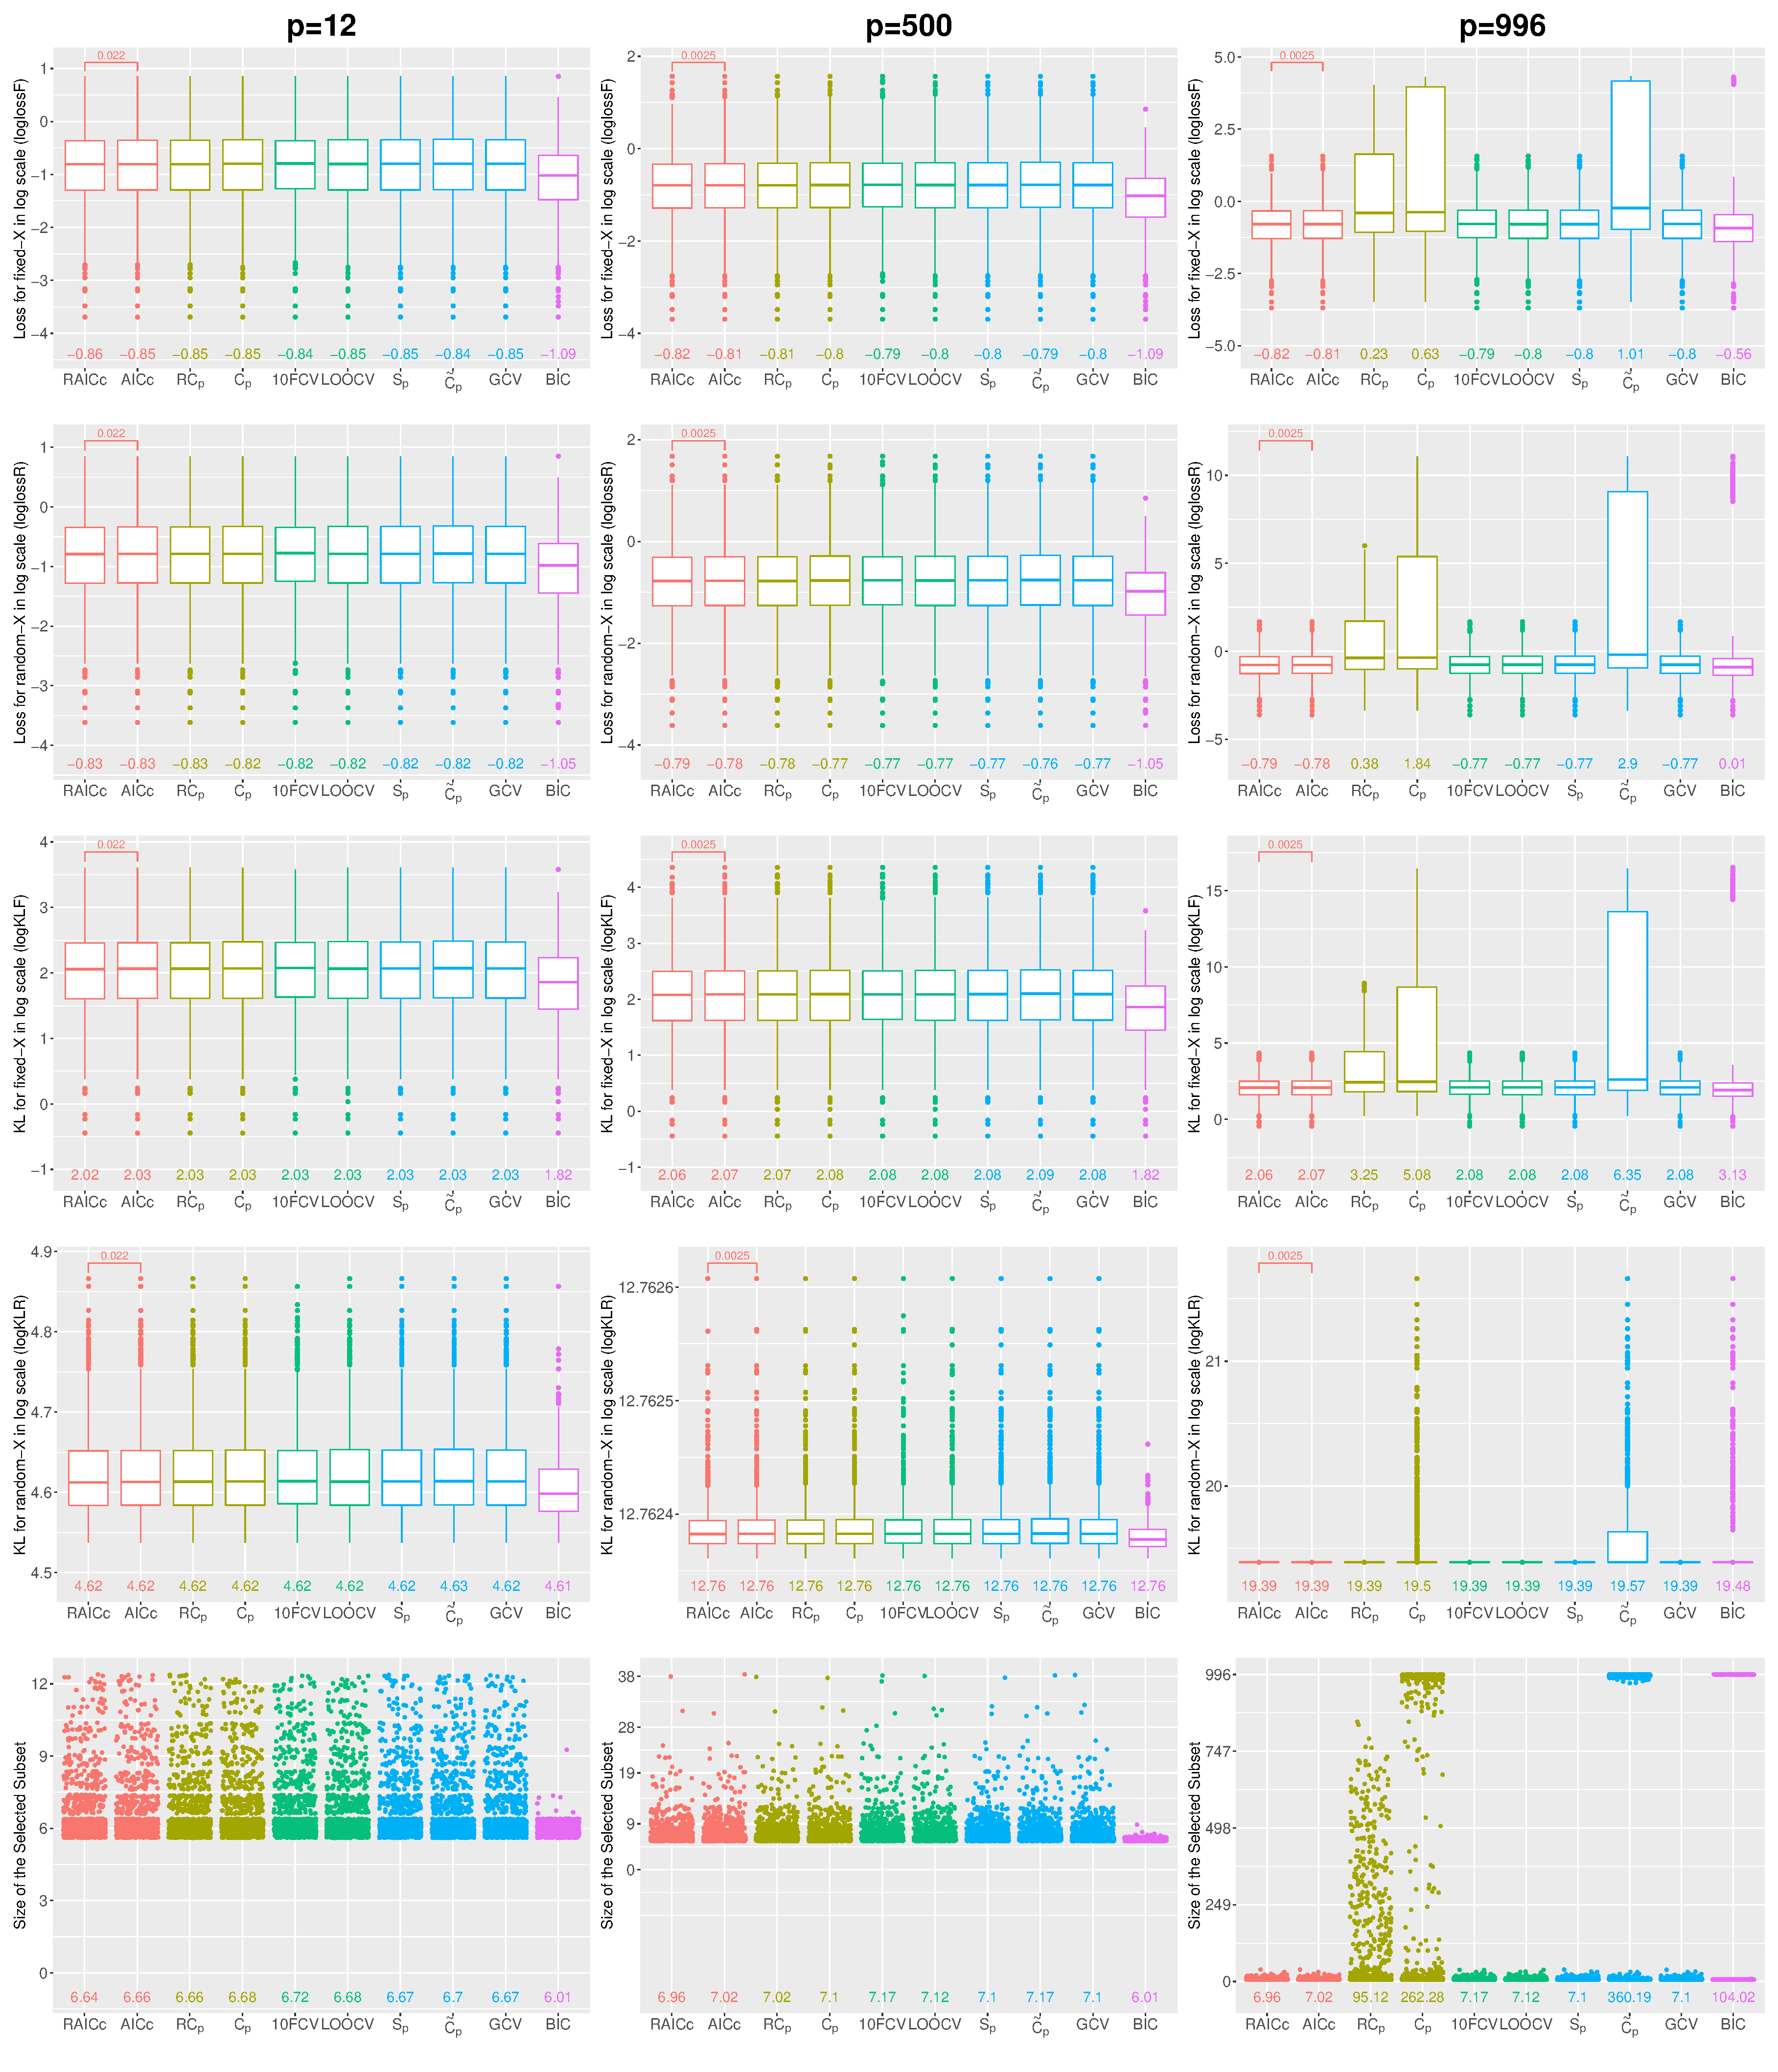
\includegraphics[width=\textwidth]{figures/supplement/fixedx/subset_selection/Sparse-Ex2_n1000_msnr_rho0.eps}
\caption{Variable selection, Fixed-X, Sparse-Ex2, $n=1000$, medium signal, and $\rho=0$.}
\end{figure}
\clearpage
\begin{figure}[!ht]
\centering
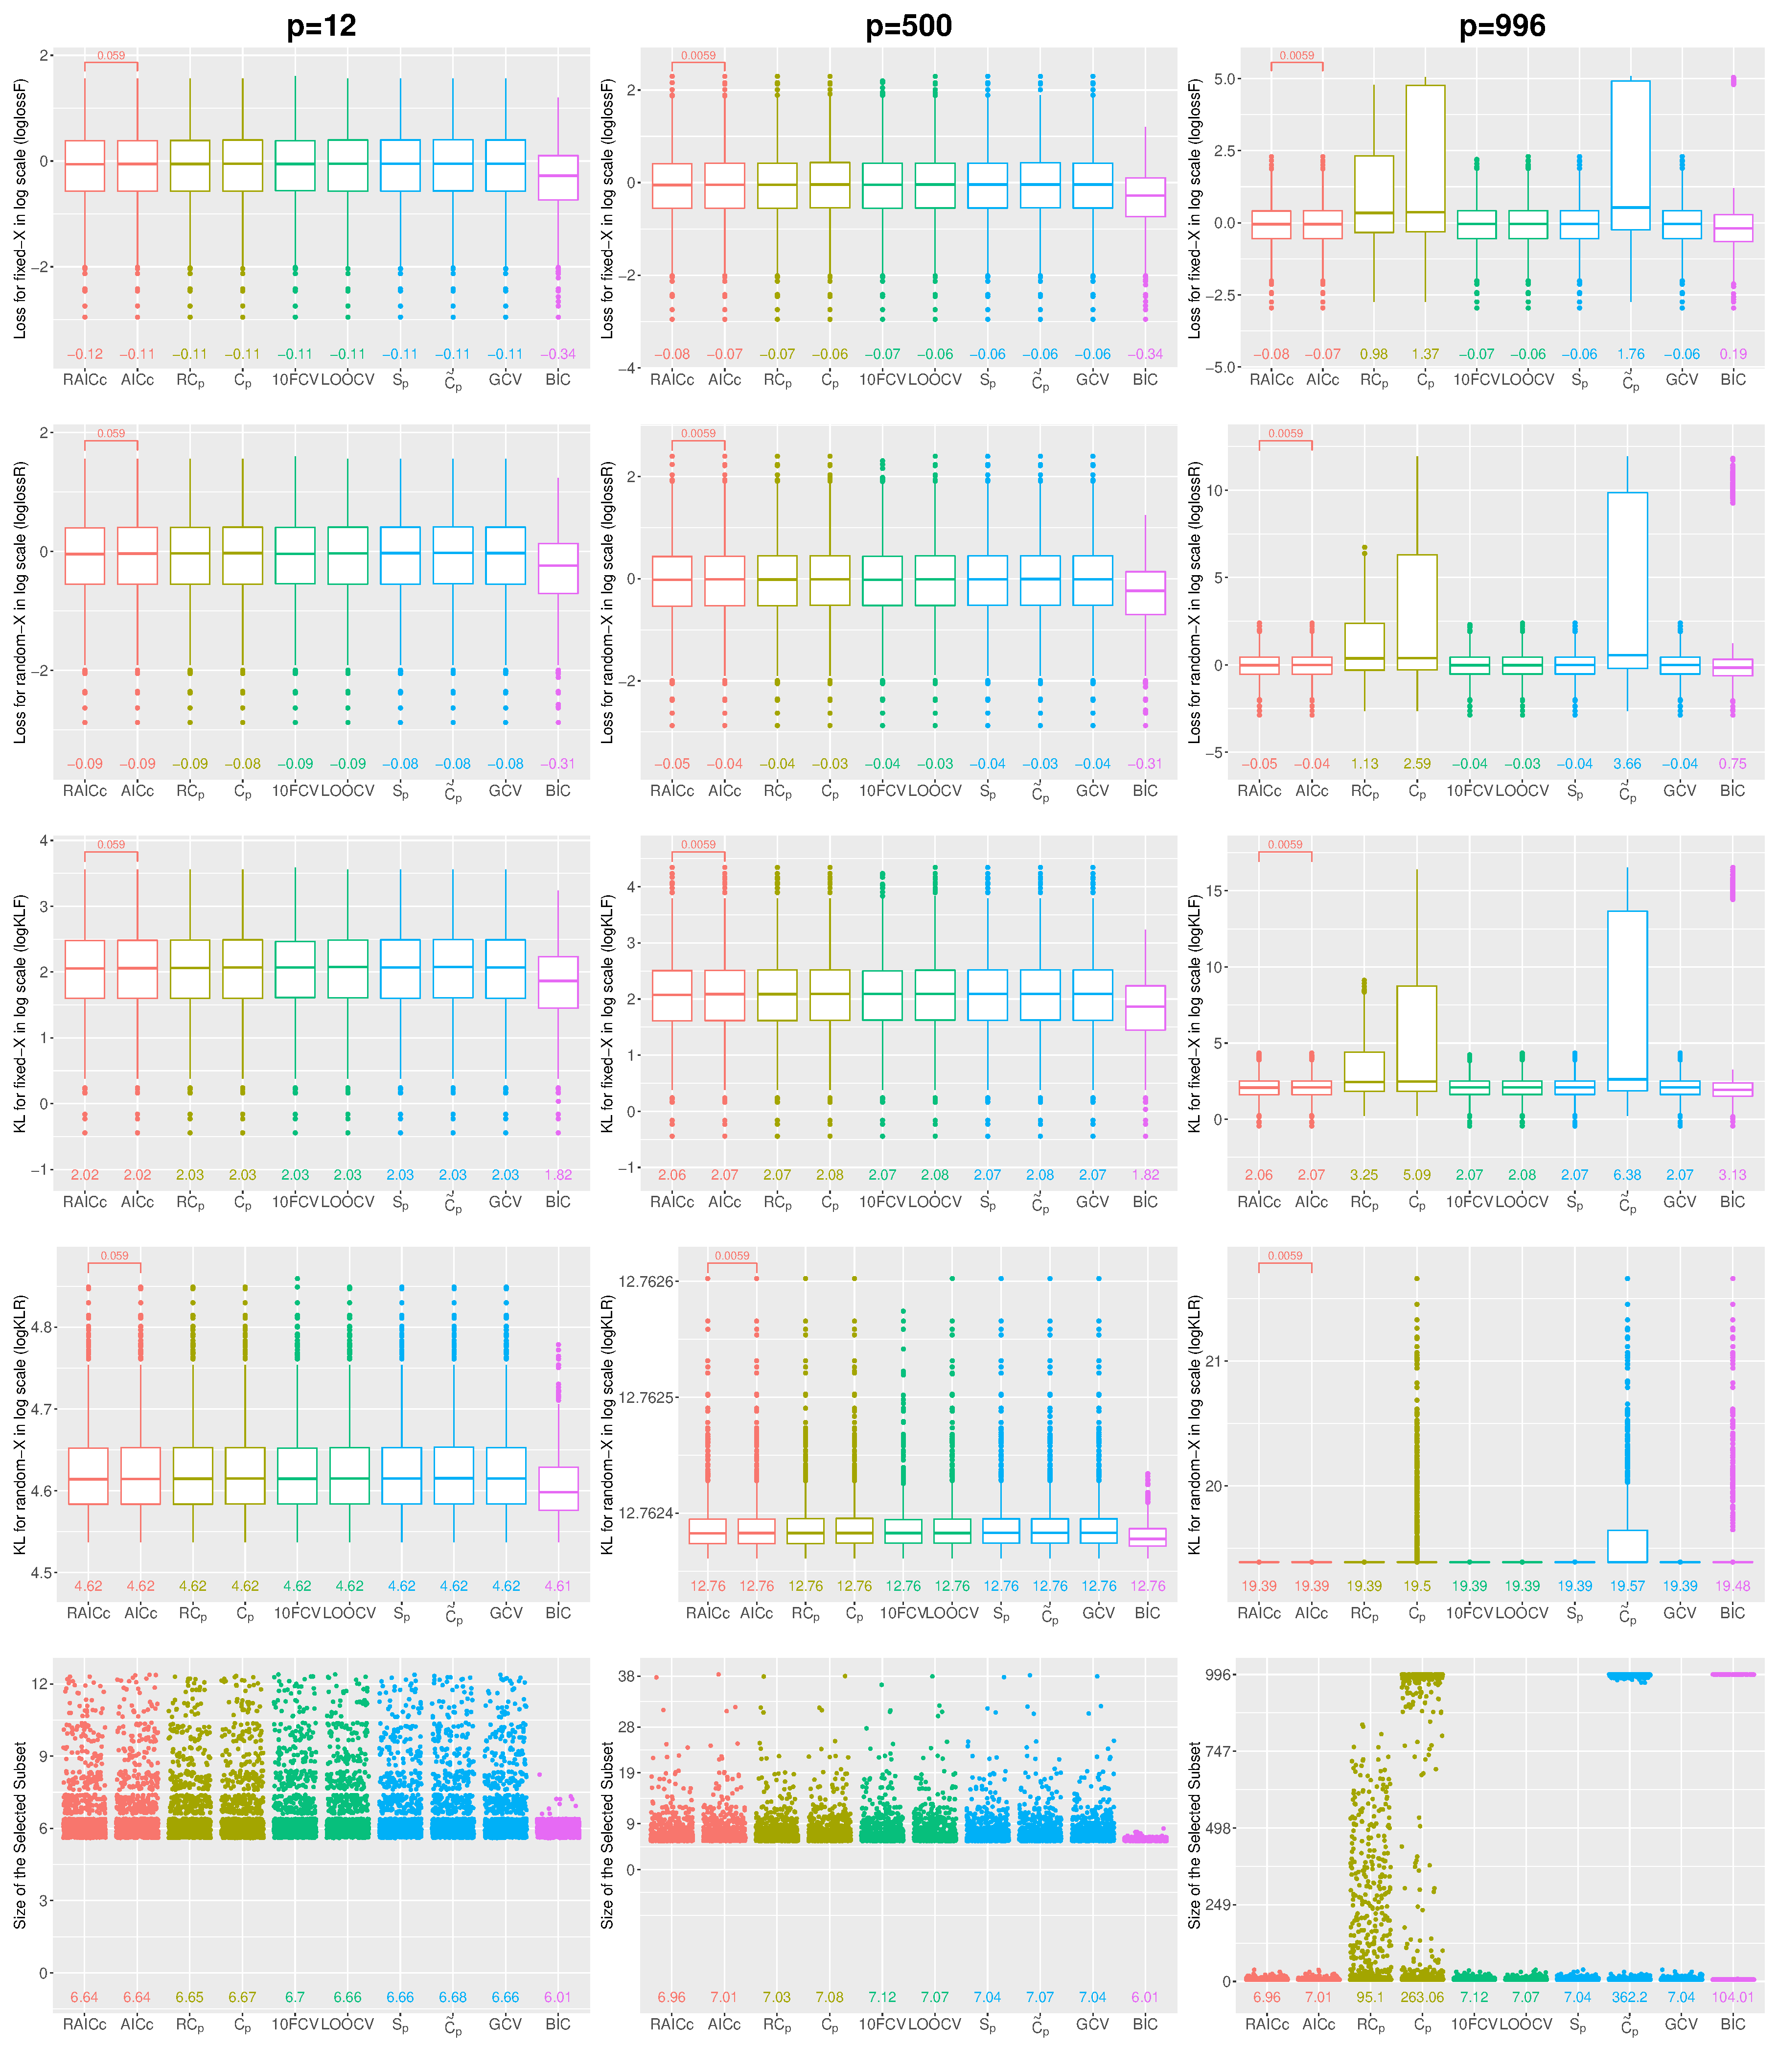
\includegraphics[width=\textwidth]{figures/supplement/fixedx/subset_selection/Sparse-Ex2_n1000_msnr_rho05.eps}
\caption{Variable selection, Fixed-X, Sparse-Ex2, $n=1000$, medium signal, and $\rho=0.5$.}
\end{figure}
\clearpage
\begin{figure}[!ht]
\centering
\includegraphics[width=\textwidth]{figures/supplement/fixedx/subset_selection/Sparse-Ex2_n1000_msnr_rho09.eps}
\caption{Variable selection, Fixed-X, Sparse-Ex2, $n=1000$, medium signal, and $\rho=0.9$.}
\end{figure}
\clearpage
\begin{figure}[!ht]
\centering
\includegraphics[width=\textwidth]{figures/supplement/fixedx/subset_selection/Sparse-Ex2_n1000_lsnr_rho0.eps}
\caption{Variable selection, Fixed-X, Sparse-Ex2, $n=1000$, low signal, and $\rho=0$.}
\end{figure}
\clearpage
\begin{figure}[!ht]
\centering
\includegraphics[width=\textwidth]{figures/supplement/fixedx/subset_selection/Sparse-Ex2_n1000_lsnr_rho05.eps}
\caption{Variable selection, Fixed-X, Sparse-Ex2, $n=1000$, low signal, and $\rho=0.5$.}
\end{figure}
\clearpage
\begin{figure}[!ht]
\centering
\includegraphics[width=\textwidth]{figures/supplement/fixedx/subset_selection/Sparse-Ex2_n1000_lsnr_rho09.eps}
\caption{Variable selection, Fixed-X, Sparse-Ex2, $n=1000$, low signal, and $\rho=0.9$.}
\end{figure}
\clearpage
\begin{figure}[!ht]
\centering
\includegraphics[width=\textwidth]{figures/supplement/fixedx/subset_selection/Dense-Ex1_n40_hsnr_rho0.eps}
\caption{Variable selection, Fixed-X, Dense-Ex1, $n=40$, high signal, and $\rho=0$.}
\end{figure}
\clearpage
\begin{figure}[!ht]
\centering
\includegraphics[width=\textwidth]{figures/supplement/fixedx/subset_selection/Dense-Ex1_n40_hsnr_rho05.eps}
\caption{Variable selection, Fixed-X, Dense-Ex1, $n=40$, high signal, and $\rho=0.5$.}
\end{figure}
\clearpage
\begin{figure}[!ht]
\centering
\includegraphics[width=\textwidth]{figures/supplement/fixedx/subset_selection/Dense-Ex1_n40_hsnr_rho09.eps}
\caption{Variable selection, Fixed-X, Dense-Ex1, $n=40$, high signal, and $\rho=0.9$.}
\end{figure}
\clearpage
\begin{figure}[!ht]
\centering
\includegraphics[width=\textwidth]{figures/supplement/fixedx/subset_selection/Dense-Ex1_n40_msnr_rho0.eps}
\caption{Variable selection, Fixed-X, Dense-Ex1, $n=40$, medium signal, and $\rho=0$.}
\end{figure}
\clearpage
\begin{figure}[!ht]
\centering
\includegraphics[width=\textwidth]{figures/supplement/fixedx/subset_selection/Dense-Ex1_n40_msnr_rho05.eps}
\caption{Variable selection, Fixed-X, Dense-Ex1, $n=40$, medium signal, and $\rho=0.5$.}
\end{figure}
\clearpage
\begin{figure}[!ht]
\centering
\includegraphics[width=\textwidth]{figures/supplement/fixedx/subset_selection/Dense-Ex1_n40_msnr_rho09.eps}
\caption{Variable selection, Fixed-X, Dense-Ex1, $n=40$, medium signal, and $\rho=0.9$.}
\end{figure}
\clearpage
\begin{figure}[!ht]
\centering
\includegraphics[width=\textwidth]{figures/supplement/fixedx/subset_selection/Dense-Ex1_n40_lsnr_rho0.eps}
\caption{Variable selection, Fixed-X, Dense-Ex1, $n=40$, low signal, and $\rho=0$.}
\end{figure}
\clearpage
\begin{figure}[!ht]
\centering
\includegraphics[width=\textwidth]{figures/supplement/fixedx/subset_selection/Dense-Ex1_n40_lsnr_rho05.eps}
\caption{Variable selection, Fixed-X, Dense-Ex1, $n=40$, low signal, and $\rho=0.5$.}
\end{figure}
\clearpage
\begin{figure}[!ht]
\centering
\includegraphics[width=\textwidth]{figures/supplement/fixedx/subset_selection/Dense-Ex1_n40_lsnr_rho09.eps}
\caption{Variable selection, Fixed-X, Dense-Ex1, $n=40$, low signal, and $\rho=0.9$.}
\end{figure}
\clearpage
\begin{figure}[!ht]
\centering
\includegraphics[width=\textwidth]{figures/supplement/fixedx/subset_selection/Dense-Ex1_n200_hsnr_rho0.eps}
\caption{Variable selection, Fixed-X, Dense-Ex1, $n=200$, high signal, and $\rho=0$.}
\end{figure}
\clearpage
\begin{figure}[!ht]
\centering
\includegraphics[width=\textwidth]{figures/supplement/fixedx/subset_selection/Dense-Ex1_n200_hsnr_rho05.eps}
\caption{Variable selection, Fixed-X, Dense-Ex1, $n=200$, high signal, and $\rho=0.5$.}
\end{figure}
\clearpage
\begin{figure}[!ht]
\centering
\includegraphics[width=\textwidth]{figures/supplement/fixedx/subset_selection/Dense-Ex1_n200_hsnr_rho09.eps}
\caption{Variable selection, Fixed-X, Dense-Ex1, $n=200$, high signal, and $\rho=0.9$.}
\end{figure}
\clearpage
\begin{figure}[!ht]
\centering
\includegraphics[width=\textwidth]{figures/supplement/fixedx/subset_selection/Dense-Ex1_n200_msnr_rho0.eps}
\caption{Variable selection, Fixed-X, Dense-Ex1, $n=200$, medium signal, and $\rho=0$.}
\end{figure}
\clearpage
\begin{figure}[!ht]
\centering
\includegraphics[width=\textwidth]{figures/supplement/fixedx/subset_selection/Dense-Ex1_n200_msnr_rho05.eps}
\caption{Variable selection, Fixed-X, Dense-Ex1, $n=200$, medium signal, and $\rho=0.5$.}
\end{figure}
\clearpage
\begin{figure}[!ht]
\centering
\includegraphics[width=\textwidth]{figures/supplement/fixedx/subset_selection/Dense-Ex1_n200_msnr_rho09.eps}
\caption{Variable selection, Fixed-X, Dense-Ex1, $n=200$, medium signal, and $\rho=0.9$.}
\end{figure}
\clearpage
\begin{figure}[!ht]
\centering
\includegraphics[width=\textwidth]{figures/supplement/fixedx/subset_selection/Dense-Ex1_n200_lsnr_rho0.eps}
\caption{Variable selection, Fixed-X, Dense-Ex1, $n=200$, low signal, and $\rho=0$.}
\end{figure}
\clearpage
\begin{figure}[!ht]
\centering
\includegraphics[width=\textwidth]{figures/supplement/fixedx/subset_selection/Dense-Ex1_n200_lsnr_rho05.eps}
\caption{Variable selection, Fixed-X, Dense-Ex1, $n=200$, low signal, and $\rho=0.5$.}
\end{figure}
\clearpage
\begin{figure}[!ht]
\centering
\includegraphics[width=\textwidth]{figures/supplement/fixedx/subset_selection/Dense-Ex1_n200_lsnr_rho09.eps}
\caption{Variable selection, Fixed-X, Dense-Ex1, $n=200$, low signal, and $\rho=0.9$.}
\end{figure}
\clearpage
\begin{figure}[!ht]
\centering
\includegraphics[width=\textwidth]{figures/supplement/fixedx/subset_selection/Dense-Ex1_n1000_hsnr_rho0.eps}
\caption{Variable selection, Fixed-X, Dense-Ex1, $n=1000$, high signal, and $\rho=0$.}
\end{figure}
\clearpage
\begin{figure}[!ht]
\centering
\includegraphics[width=\textwidth]{figures/supplement/fixedx/subset_selection/Dense-Ex1_n1000_hsnr_rho05.eps}
\caption{Variable selection, Fixed-X, Dense-Ex1, $n=1000$, high signal, and $\rho=0.5$.}
\end{figure}
\clearpage
\begin{figure}[!ht]
\centering
\includegraphics[width=\textwidth]{figures/supplement/fixedx/subset_selection/Dense-Ex1_n1000_hsnr_rho09.eps}
\caption{Variable selection, Fixed-X, Dense-Ex1, $n=1000$, high signal, and $\rho=0.9$.}
\end{figure}
\clearpage
\begin{figure}[!ht]
\centering
\includegraphics[width=\textwidth]{figures/supplement/fixedx/subset_selection/Dense-Ex1_n1000_msnr_rho0.eps}
\caption{Variable selection, Fixed-X, Dense-Ex1, $n=1000$, medium signal, and $\rho=0$.}
\end{figure}
\clearpage
\begin{figure}[!ht]
\centering
\includegraphics[width=\textwidth]{figures/supplement/fixedx/subset_selection/Dense-Ex1_n1000_msnr_rho05.eps}
\caption{Variable selection, Fixed-X, Dense-Ex1, $n=1000$, medium signal, and $\rho=0.5$.}
\end{figure}
\clearpage
\begin{figure}[!ht]
\centering
\includegraphics[width=\textwidth]{figures/supplement/fixedx/subset_selection/Dense-Ex1_n1000_msnr_rho09.eps}
\caption{Variable selection, Fixed-X, Dense-Ex1, $n=1000$, medium signal, and $\rho=0.9$.}
\end{figure}
\clearpage
\begin{figure}[!ht]
\centering
\includegraphics[width=\textwidth]{figures/supplement/fixedx/subset_selection/Dense-Ex1_n1000_lsnr_rho0.eps}
\caption{Variable selection, Fixed-X, Dense-Ex1, $n=1000$, low signal, and $\rho=0$.}
\end{figure}
\clearpage
\begin{figure}[!ht]
\centering
\includegraphics[width=\textwidth]{figures/supplement/fixedx/subset_selection/Dense-Ex1_n1000_lsnr_rho05.eps}
\caption{Variable selection, Fixed-X, Dense-Ex1, $n=1000$, low signal, and $\rho=0.5$.}
\end{figure}
\clearpage
\begin{figure}[!ht]
\centering
\includegraphics[width=\textwidth]{figures/supplement/fixedx/subset_selection/Dense-Ex1_n1000_lsnr_rho09.eps}
\caption{Variable selection, Fixed-X, Dense-Ex1, $n=1000$, low signal, and $\rho=0.9$.}
\end{figure}
\clearpage
\begin{figure}[!ht]
\centering
\includegraphics[width=\textwidth]{figures/supplement/randomx/subset_selection/Sparse-Ex1_n40_hsnr_rho0.eps}
\caption{Variable selection, Random-X, Sparse-Ex1, $n=40$, high signal, and $\rho=0$.}
\end{figure}
\clearpage
\begin{figure}[!ht]
\centering
\includegraphics[width=\textwidth]{figures/supplement/randomx/subset_selection/Sparse-Ex1_n40_hsnr_rho05.eps}
\caption{Variable selection, Random-X, Sparse-Ex1, $n=40$, high signal, and $\rho=0.5$.}
\end{figure}
\clearpage
\begin{figure}[!ht]
\centering
\includegraphics[width=\textwidth]{figures/supplement/randomx/subset_selection/Sparse-Ex1_n40_hsnr_rho09.eps}
\caption{Variable selection, Random-X, Sparse-Ex1, $n=40$, high signal, and $\rho=0.9$.}
\end{figure}
\clearpage
\begin{figure}[!ht]
\centering
\includegraphics[width=\textwidth]{figures/supplement/randomx/subset_selection/Sparse-Ex1_n40_msnr_rho0.eps}
\caption{Variable selection, Random-X, Sparse-Ex1, $n=40$, medium signal, and $\rho=0$.}
\end{figure}
\clearpage
\begin{figure}[!ht]
\centering
\includegraphics[width=\textwidth]{figures/supplement/randomx/subset_selection/Sparse-Ex1_n40_msnr_rho05.eps}
\caption{Variable selection, Random-X, Sparse-Ex1, $n=40$, medium signal, and $\rho=0.5$.}
\end{figure}
\clearpage
\begin{figure}[!ht]
\centering
\includegraphics[width=\textwidth]{figures/supplement/randomx/subset_selection/Sparse-Ex1_n40_msnr_rho09.eps}
\caption{Variable selection, Random-X, Sparse-Ex1, $n=40$, medium signal, and $\rho=0.9$.}
\end{figure}
\clearpage
\begin{figure}[!ht]
\centering
\includegraphics[width=\textwidth]{figures/supplement/randomx/subset_selection/Sparse-Ex1_n40_lsnr_rho0.eps}
\caption{Variable selection, Random-X, Sparse-Ex1, $n=40$, low signal, and $\rho=0$.}
\end{figure}
\clearpage
\begin{figure}[!ht]
\centering
\includegraphics[width=\textwidth]{figures/supplement/randomx/subset_selection/Sparse-Ex1_n40_lsnr_rho05.eps}
\caption{Variable selection, Random-X, Sparse-Ex1, $n=40$, low signal, and $\rho=0.5$.}
\end{figure}
\clearpage
\begin{figure}[!ht]
\centering
\includegraphics[width=\textwidth]{figures/supplement/randomx/subset_selection/Sparse-Ex1_n40_lsnr_rho09.eps}
\caption{Variable selection, Random-X, Sparse-Ex1, $n=40$, low signal, and $\rho=0.9$.}
\end{figure}
\clearpage
\begin{figure}[!ht]
\centering
\includegraphics[width=\textwidth]{figures/supplement/randomx/subset_selection/Sparse-Ex1_n200_hsnr_rho0.eps}
\caption{Variable selection, Random-X, Sparse-Ex1, $n=200$, high signal, and $\rho=0$.}
\end{figure}
\clearpage
\begin{figure}[!ht]
\centering
\includegraphics[width=\textwidth]{figures/supplement/randomx/subset_selection/Sparse-Ex1_n200_hsnr_rho05.eps}
\caption{Variable selection, Random-X, Sparse-Ex1, $n=200$, high signal, and $\rho=0.5$.}
\end{figure}
\clearpage
\begin{figure}[!ht]
\centering
\includegraphics[width=\textwidth]{figures/supplement/randomx/subset_selection/Sparse-Ex1_n200_hsnr_rho09.eps}
\caption{Variable selection, Random-X, Sparse-Ex1, $n=200$, high signal, and $\rho=0.9$.}
\end{figure}
\clearpage
\begin{figure}[!ht]
\centering
\includegraphics[width=\textwidth]{figures/supplement/randomx/subset_selection/Sparse-Ex1_n200_msnr_rho0.eps}
\caption{Variable selection, Random-X, Sparse-Ex1, $n=200$, medium signal, and $\rho=0$.}
\end{figure}
\clearpage
\begin{figure}[!ht]
\centering
\includegraphics[width=\textwidth]{figures/supplement/randomx/subset_selection/Sparse-Ex1_n200_msnr_rho05.eps}
\caption{Variable selection, Random-X, Sparse-Ex1, $n=200$, medium signal, and $\rho=0.5$.}
\end{figure}
\clearpage
\begin{figure}[!ht]
\centering
\includegraphics[width=\textwidth]{figures/supplement/randomx/subset_selection/Sparse-Ex1_n200_msnr_rho09.eps}
\caption{Variable selection, Random-X, Sparse-Ex1, $n=200$, medium signal, and $\rho=0.9$.}
\end{figure}
\clearpage
\begin{figure}[!ht]
\centering
\includegraphics[width=\textwidth]{figures/supplement/randomx/subset_selection/Sparse-Ex1_n200_lsnr_rho0.eps}
\caption{Variable selection, Random-X, Sparse-Ex1, $n=200$, low signal, and $\rho=0$.}
\end{figure}
\clearpage
\begin{figure}[!ht]
\centering
\includegraphics[width=\textwidth]{figures/supplement/randomx/subset_selection/Sparse-Ex1_n200_lsnr_rho05.eps}
\caption{Variable selection, Random-X, Sparse-Ex1, $n=200$, low signal, and $\rho=0.5$.}
\end{figure}
\clearpage
\begin{figure}[!ht]
\centering
\includegraphics[width=\textwidth]{figures/supplement/randomx/subset_selection/Sparse-Ex1_n200_lsnr_rho09.eps}
\caption{Variable selection, Random-X, Sparse-Ex1, $n=200$, low signal, and $\rho=0.9$.}
\end{figure}
\clearpage
\begin{figure}[!ht]
\centering
\includegraphics[width=\textwidth]{figures/supplement/randomx/subset_selection/Sparse-Ex1_n1000_hsnr_rho0.eps}
\caption{Variable selection, Random-X, Sparse-Ex1, $n=1000$, high signal, and $\rho=0$.}
\end{figure}
\clearpage
\begin{figure}[!ht]
\centering
\includegraphics[width=\textwidth]{figures/supplement/randomx/subset_selection/Sparse-Ex1_n1000_hsnr_rho05.eps}
\caption{Variable selection, Random-X, Sparse-Ex1, $n=1000$, high signal, and $\rho=0.5$.}
\end{figure}
\clearpage
\begin{figure}[!ht]
\centering
\includegraphics[width=\textwidth]{figures/supplement/randomx/subset_selection/Sparse-Ex1_n1000_hsnr_rho09.eps}
\caption{Variable selection, Random-X, Sparse-Ex1, $n=1000$, high signal, and $\rho=0.9$.}
\end{figure}
\clearpage
\begin{figure}[!ht]
\centering
\includegraphics[width=\textwidth]{figures/supplement/randomx/subset_selection/Sparse-Ex1_n1000_msnr_rho0.eps}
\caption{Variable selection, Random-X, Sparse-Ex1, $n=1000$, medium signal, and $\rho=0$.}
\end{figure}
\clearpage
\begin{figure}[!ht]
\centering
\includegraphics[width=\textwidth]{figures/supplement/randomx/subset_selection/Sparse-Ex1_n1000_msnr_rho05.eps}
\caption{Variable selection, Random-X, Sparse-Ex1, $n=1000$, medium signal, and $\rho=0.5$.}
\end{figure}
\clearpage
\begin{figure}[!ht]
\centering
\includegraphics[width=\textwidth]{figures/supplement/randomx/subset_selection/Sparse-Ex1_n1000_msnr_rho09.eps}
\caption{Variable selection, Random-X, Sparse-Ex1, $n=1000$, medium signal, and $\rho=0.9$.}
\end{figure}
\clearpage
\begin{figure}[!ht]
\centering
\includegraphics[width=\textwidth]{figures/supplement/randomx/subset_selection/Sparse-Ex1_n1000_lsnr_rho0.eps}
\caption{Variable selection, Random-X, Sparse-Ex1, $n=1000$, low signal, and $\rho=0$.}
\end{figure}
\clearpage
\begin{figure}[!ht]
\centering
\includegraphics[width=\textwidth]{figures/supplement/randomx/subset_selection/Sparse-Ex1_n1000_lsnr_rho05.eps}
\caption{Variable selection, Random-X, Sparse-Ex1, $n=1000$, low signal, and $\rho=0.5$.}
\end{figure}
\clearpage
\begin{figure}[!ht]
\centering
\includegraphics[width=\textwidth]{figures/supplement/randomx/subset_selection/Sparse-Ex1_n1000_lsnr_rho09.eps}
\caption{Variable selection, Random-X, Sparse-Ex1, $n=1000$, low signal, and $\rho=0.9$.}
\end{figure}
\clearpage
\begin{figure}[!ht]
\centering
\includegraphics[width=\textwidth]{figures/supplement/randomx/subset_selection/Sparse-Ex2_n40_hsnr_rho0.eps}
\caption{Variable selection, Random-X, Sparse-Ex2, $n=40$, high signal, and $\rho=0$.}
\end{figure}
\clearpage
\begin{figure}[!ht]
\centering
\includegraphics[width=\textwidth]{figures/supplement/randomx/subset_selection/Sparse-Ex2_n40_hsnr_rho05.eps}
\caption{Variable selection, Random-X, Sparse-Ex2, $n=40$, high signal, and $\rho=0.5$.}
\end{figure}
\clearpage
\begin{figure}[!ht]
\centering
\includegraphics[width=\textwidth]{figures/supplement/randomx/subset_selection/Sparse-Ex2_n40_hsnr_rho09.eps}
\caption{Variable selection, Random-X, Sparse-Ex2, $n=40$, high signal, and $\rho=0.9$.}
\end{figure}
\clearpage
\begin{figure}[!ht]
\centering
\includegraphics[width=\textwidth]{figures/supplement/randomx/subset_selection/Sparse-Ex2_n40_msnr_rho0.eps}
\caption{Variable selection, Random-X, Sparse-Ex2, $n=40$, medium signal, and $\rho=0$.}
\end{figure}
\clearpage
\begin{figure}[!ht]
\centering
\includegraphics[width=\textwidth]{figures/supplement/randomx/subset_selection/Sparse-Ex2_n40_msnr_rho05.eps}
\caption{Variable selection, Random-X, Sparse-Ex2, $n=40$, medium signal, and $\rho=0.5$.}
\end{figure}
\clearpage
\begin{figure}[!ht]
\centering
\includegraphics[width=\textwidth]{figures/supplement/randomx/subset_selection/Sparse-Ex2_n40_msnr_rho09.eps}
\caption{Variable selection, Random-X, Sparse-Ex2, $n=40$, medium signal, and $\rho=0.9$.}
\end{figure}
\clearpage
\begin{figure}[!ht]
\centering
\includegraphics[width=\textwidth]{figures/supplement/randomx/subset_selection/Sparse-Ex2_n40_lsnr_rho0.eps}
\caption{Variable selection, Random-X, Sparse-Ex2, $n=40$, low signal, and $\rho=0$.}
\end{figure}
\clearpage
\begin{figure}[!ht]
\centering
\includegraphics[width=\textwidth]{figures/supplement/randomx/subset_selection/Sparse-Ex2_n40_lsnr_rho05.eps}
\caption{Variable selection, Random-X, Sparse-Ex2, $n=40$, low signal, and $\rho=0.5$.}
\end{figure}
\clearpage
\begin{figure}[!ht]
\centering
\includegraphics[width=\textwidth]{figures/supplement/randomx/subset_selection/Sparse-Ex2_n40_lsnr_rho09.eps}
\caption{Variable selection, Random-X, Sparse-Ex2, $n=40$, low signal, and $\rho=0.9$.}
\end{figure}
\clearpage
\begin{figure}[!ht]
\centering
\includegraphics[width=\textwidth]{figures/supplement/randomx/subset_selection/Sparse-Ex2_n200_hsnr_rho0.eps}
\caption{Variable selection, Random-X, Sparse-Ex2, $n=200$, high signal, and $\rho=0$.}
\end{figure}
\clearpage
\begin{figure}[!ht]
\centering
\includegraphics[width=\textwidth]{figures/supplement/randomx/subset_selection/Sparse-Ex2_n200_hsnr_rho05.eps}
\caption{Variable selection, Random-X, Sparse-Ex2, $n=200$, high signal, and $\rho=0.5$.}
\end{figure}
\clearpage
\begin{figure}[!ht]
\centering
\includegraphics[width=\textwidth]{figures/supplement/randomx/subset_selection/Sparse-Ex2_n200_hsnr_rho09.eps}
\caption{Variable selection, Random-X, Sparse-Ex2, $n=200$, high signal, and $\rho=0.9$.}
\end{figure}
\clearpage
\begin{figure}[!ht]
\centering
\includegraphics[width=\textwidth]{figures/supplement/randomx/subset_selection/Sparse-Ex2_n200_msnr_rho0.eps}
\caption{Variable selection, Random-X, Sparse-Ex2, $n=200$, medium signal, and $\rho=0$.}
\end{figure}
\clearpage
\begin{figure}[!ht]
\centering
\includegraphics[width=\textwidth]{figures/supplement/randomx/subset_selection/Sparse-Ex2_n200_msnr_rho05.eps}
\caption{Variable selection, Random-X, Sparse-Ex2, $n=200$, medium signal, and $\rho=0.5$.}
\end{figure}
\clearpage
\begin{figure}[!ht]
\centering
\includegraphics[width=\textwidth]{figures/supplement/randomx/subset_selection/Sparse-Ex2_n200_msnr_rho09.eps}
\caption{Variable selection, Random-X, Sparse-Ex2, $n=200$, medium signal, and $\rho=0.9$.}
\end{figure}
\clearpage
\begin{figure}[!ht]
\centering
\includegraphics[width=\textwidth]{figures/supplement/randomx/subset_selection/Sparse-Ex2_n200_lsnr_rho0.eps}
\caption{Variable selection, Random-X, Sparse-Ex2, $n=200$, low signal, and $\rho=0$.}
\end{figure}
\clearpage
\begin{figure}[!ht]
\centering
\includegraphics[width=\textwidth]{figures/supplement/randomx/subset_selection/Sparse-Ex2_n200_lsnr_rho05.eps}
\caption{Variable selection, Random-X, Sparse-Ex2, $n=200$, low signal, and $\rho=0.5$.}
\end{figure}
\clearpage
\begin{figure}[!ht]
\centering
\includegraphics[width=\textwidth]{figures/supplement/randomx/subset_selection/Sparse-Ex2_n200_lsnr_rho09.eps}
\caption{Variable selection, Random-X, Sparse-Ex2, $n=200$, low signal, and $\rho=0.9$.}
\end{figure}
\clearpage
\begin{figure}[!ht]
\centering
\includegraphics[width=\textwidth]{figures/supplement/randomx/subset_selection/Sparse-Ex2_n1000_hsnr_rho0.eps}
\caption{Variable selection, Random-X, Sparse-Ex2, $n=1000$, high signal, and $\rho=0$.}
\end{figure}
\clearpage
\begin{figure}[!ht]
\centering
\includegraphics[width=\textwidth]{figures/supplement/randomx/subset_selection/Sparse-Ex2_n1000_hsnr_rho05.eps}
\caption{Variable selection, Random-X, Sparse-Ex2, $n=1000$, high signal, and $\rho=0.5$.}
\end{figure}
\clearpage
\begin{figure}[!ht]
\centering
\includegraphics[width=\textwidth]{figures/supplement/randomx/subset_selection/Sparse-Ex2_n1000_hsnr_rho09.eps}
\caption{Variable selection, Random-X, Sparse-Ex2, $n=1000$, high signal, and $\rho=0.9$.}
\end{figure}
\clearpage
\begin{figure}[!ht]
\centering
\includegraphics[width=\textwidth]{figures/supplement/randomx/subset_selection/Sparse-Ex2_n1000_msnr_rho0.eps}
\caption{Variable selection, Random-X, Sparse-Ex2, $n=1000$, medium signal, and $\rho=0$.}
\end{figure}
\clearpage
\begin{figure}[!ht]
\centering
\includegraphics[width=\textwidth]{figures/supplement/randomx/subset_selection/Sparse-Ex2_n1000_msnr_rho05.eps}
\caption{Variable selection, Random-X, Sparse-Ex2, $n=1000$, medium signal, and $\rho=0.5$.}
\end{figure}
\clearpage
\begin{figure}[!ht]
\centering
\includegraphics[width=\textwidth]{figures/supplement/randomx/subset_selection/Sparse-Ex2_n1000_msnr_rho09.eps}
\caption{Variable selection, Random-X, Sparse-Ex2, $n=1000$, medium signal, and $\rho=0.9$.}
\end{figure}
\clearpage
\begin{figure}[!ht]
\centering
\includegraphics[width=\textwidth]{figures/supplement/randomx/subset_selection/Sparse-Ex2_n1000_lsnr_rho0.eps}
\caption{Variable selection, Random-X, Sparse-Ex2, $n=1000$, low signal, and $\rho=0$.}
\end{figure}
\clearpage
\begin{figure}[!ht]
\centering
\includegraphics[width=\textwidth]{figures/supplement/randomx/subset_selection/Sparse-Ex2_n1000_lsnr_rho05.eps}
\caption{Variable selection, Random-X, Sparse-Ex2, $n=1000$, low signal, and $\rho=0.5$.}
\end{figure}
\clearpage
\begin{figure}[!ht]
\centering
\includegraphics[width=\textwidth]{figures/supplement/randomx/subset_selection/Sparse-Ex2_n1000_lsnr_rho09.eps}
\caption{Variable selection, Random-X, Sparse-Ex2, $n=1000$, low signal, and $\rho=0.9$.}
\end{figure}
\clearpage
\begin{figure}[!ht]
\centering
\includegraphics[width=\textwidth]{figures/supplement/randomx/subset_selection/Dense-Ex1_n40_hsnr_rho0.eps}
\caption{Variable selection, Random-X, Dense-Ex1, $n=40$, high signal, and $\rho=0$.}
\end{figure}
\clearpage
\begin{figure}[!ht]
\centering
\includegraphics[width=\textwidth]{figures/supplement/randomx/subset_selection/Dense-Ex1_n40_hsnr_rho05.eps}
\caption{Variable selection, Random-X, Dense-Ex1, $n=40$, high signal, and $\rho=0.5$.}
\end{figure}
\clearpage
\begin{figure}[!ht]
\centering
\includegraphics[width=\textwidth]{figures/supplement/randomx/subset_selection/Dense-Ex1_n40_hsnr_rho09.eps}
\caption{Variable selection, Random-X, Dense-Ex1, $n=40$, high signal, and $\rho=0.9$.}
\end{figure}
\clearpage
\begin{figure}[!ht]
\centering
\includegraphics[width=\textwidth]{figures/supplement/randomx/subset_selection/Dense-Ex1_n40_msnr_rho0.eps}
\caption{Variable selection, Random-X, Dense-Ex1, $n=40$, medium signal, and $\rho=0$.}
\end{figure}
\clearpage
\begin{figure}[!ht]
\centering
\includegraphics[width=\textwidth]{figures/supplement/randomx/subset_selection/Dense-Ex1_n40_msnr_rho05.eps}
\caption{Variable selection, Random-X, Dense-Ex1, $n=40$, medium signal, and $\rho=0.5$.}
\end{figure}
\clearpage
\begin{figure}[!ht]
\centering
\includegraphics[width=\textwidth]{figures/supplement/randomx/subset_selection/Dense-Ex1_n40_msnr_rho09.eps}
\caption{Variable selection, Random-X, Dense-Ex1, $n=40$, medium signal, and $\rho=0.9$.}
\end{figure}
\clearpage
\begin{figure}[!ht]
\centering
\includegraphics[width=\textwidth]{figures/supplement/randomx/subset_selection/Dense-Ex1_n40_lsnr_rho0.eps}
\caption{Variable selection, Random-X, Dense-Ex1, $n=40$, low signal, and $\rho=0$.}
\end{figure}
\clearpage
\begin{figure}[!ht]
\centering
\includegraphics[width=\textwidth]{figures/supplement/randomx/subset_selection/Dense-Ex1_n40_lsnr_rho05.eps}
\caption{Variable selection, Random-X, Dense-Ex1, $n=40$, low signal, and $\rho=0.5$.}
\end{figure}
\clearpage
\begin{figure}[!ht]
\centering
\includegraphics[width=\textwidth]{figures/supplement/randomx/subset_selection/Dense-Ex1_n40_lsnr_rho09.eps}
\caption{Variable selection, Random-X, Dense-Ex1, $n=40$, low signal, and $\rho=0.9$.}
\end{figure}
\clearpage
\begin{figure}[!ht]
\centering
\includegraphics[width=\textwidth]{figures/supplement/randomx/subset_selection/Dense-Ex1_n200_hsnr_rho0.eps}
\caption{Variable selection, Random-X, Dense-Ex1, $n=200$, high signal, and $\rho=0$.}
\end{figure}
\clearpage
\begin{figure}[!ht]
\centering
\includegraphics[width=\textwidth]{figures/supplement/randomx/subset_selection/Dense-Ex1_n200_hsnr_rho05.eps}
\caption{Variable selection, Random-X, Dense-Ex1, $n=200$, high signal, and $\rho=0.5$.}
\end{figure}
\clearpage
\begin{figure}[!ht]
\centering
\includegraphics[width=\textwidth]{figures/supplement/randomx/subset_selection/Dense-Ex1_n200_hsnr_rho09.eps}
\caption{Variable selection, Random-X, Dense-Ex1, $n=200$, high signal, and $\rho=0.9$.}
\end{figure}
\clearpage
\begin{figure}[!ht]
\centering
\includegraphics[width=\textwidth]{figures/supplement/randomx/subset_selection/Dense-Ex1_n200_msnr_rho0.eps}
\caption{Variable selection, Random-X, Dense-Ex1, $n=200$, medium signal, and $\rho=0$.}
\end{figure}
\clearpage
\begin{figure}[!ht]
\centering
\includegraphics[width=\textwidth]{figures/supplement/randomx/subset_selection/Dense-Ex1_n200_msnr_rho05.eps}
\caption{Variable selection, Random-X, Dense-Ex1, $n=200$, medium signal, and $\rho=0.5$.}
\end{figure}
\clearpage
\begin{figure}[!ht]
\centering
\includegraphics[width=\textwidth]{figures/supplement/randomx/subset_selection/Dense-Ex1_n200_msnr_rho09.eps}
\caption{Variable selection, Random-X, Dense-Ex1, $n=200$, medium signal, and $\rho=0.9$.}
\end{figure}
\clearpage
\begin{figure}[!ht]
\centering
\includegraphics[width=\textwidth]{figures/supplement/randomx/subset_selection/Dense-Ex1_n200_lsnr_rho0.eps}
\caption{Variable selection, Random-X, Dense-Ex1, $n=200$, low signal, and $\rho=0$.}
\end{figure}
\clearpage
\begin{figure}[!ht]
\centering
\includegraphics[width=\textwidth]{figures/supplement/randomx/subset_selection/Dense-Ex1_n200_lsnr_rho05.eps}
\caption{Variable selection, Random-X, Dense-Ex1, $n=200$, low signal, and $\rho=0.5$.}
\end{figure}
\clearpage
\begin{figure}[!ht]
\centering
\includegraphics[width=\textwidth]{figures/supplement/randomx/subset_selection/Dense-Ex1_n200_lsnr_rho09.eps}
\caption{Variable selection, Random-X, Dense-Ex1, $n=200$, low signal, and $\rho=0.9$.}
\end{figure}
\clearpage
\begin{figure}[!ht]
\centering
\includegraphics[width=\textwidth]{figures/supplement/randomx/subset_selection/Dense-Ex1_n1000_hsnr_rho0.eps}
\caption{Variable selection, Random-X, Dense-Ex1, $n=1000$, high signal, and $\rho=0$.}
\end{figure}
\clearpage
\begin{figure}[!ht]
\centering
\includegraphics[width=\textwidth]{figures/supplement/randomx/subset_selection/Dense-Ex1_n1000_hsnr_rho05.eps}
\caption{Variable selection, Random-X, Dense-Ex1, $n=1000$, high signal, and $\rho=0.5$.}
\end{figure}
\clearpage
\begin{figure}[!ht]
\centering
\includegraphics[width=\textwidth]{figures/supplement/randomx/subset_selection/Dense-Ex1_n1000_hsnr_rho09.eps}
\caption{Variable selection, Random-X, Dense-Ex1, $n=1000$, high signal, and $\rho=0.9$.}
\end{figure}
\clearpage
\begin{figure}[!ht]
\centering
\includegraphics[width=\textwidth]{figures/supplement/randomx/subset_selection/Dense-Ex1_n1000_msnr_rho0.eps}
\caption{Variable selection, Random-X, Dense-Ex1, $n=1000$, medium signal, and $\rho=0$.}
\end{figure}
\clearpage
\begin{figure}[!ht]
\centering
\includegraphics[width=\textwidth]{figures/supplement/randomx/subset_selection/Dense-Ex1_n1000_msnr_rho05.eps}
\caption{Variable selection, Random-X, Dense-Ex1, $n=1000$, medium signal, and $\rho=0.5$.}
\end{figure}
\clearpage
\begin{figure}[!ht]
\centering
\includegraphics[width=\textwidth]{figures/supplement/randomx/subset_selection/Dense-Ex1_n1000_msnr_rho09.eps}
\caption{Variable selection, Random-X, Dense-Ex1, $n=1000$, medium signal, and $\rho=0.9$.}
\end{figure}
\clearpage
\begin{figure}[!ht]
\centering
\includegraphics[width=\textwidth]{figures/supplement/randomx/subset_selection/Dense-Ex1_n1000_lsnr_rho0.eps}
\caption{Variable selection, Random-X, Dense-Ex1, $n=1000$, low signal, and $\rho=0$.}
\end{figure}
\clearpage
\begin{figure}[!ht]
\centering
\includegraphics[width=\textwidth]{figures/supplement/randomx/subset_selection/Dense-Ex1_n1000_lsnr_rho05.eps}
\caption{Variable selection, Random-X, Dense-Ex1, $n=1000$, low signal, and $\rho=0.5$.}
\end{figure}
\clearpage
\begin{figure}[!ht]
\centering
\includegraphics[width=\textwidth]{figures/supplement/randomx/subset_selection/Dense-Ex1_n1000_lsnr_rho09.eps}
\caption{Variable selection, Random-X, Dense-Ex1, $n=1000$, low signal, and $\rho=0.9$.}
\end{figure}
\clearpage

\begin{figure}[!ht]
\centering
\includegraphics[width=\textwidth]{figures/supplement/fixedx/general_restriction/Ex1_n10_hsnr.eps}
\caption{General restriction, Fixed-X, Ex1, $n=10$, and high signal.}
\end{figure}
\clearpage
\begin{figure}[!ht]
\centering
\includegraphics[width=\textwidth]{figures/supplement/fixedx/general_restriction/Ex1_n10_msnr.eps}
\caption{General restriction, Fixed-X, Ex1, $n=10$, and medium signal.}
\end{figure}
\clearpage
\begin{figure}[!ht]
\centering
\includegraphics[width=\textwidth]{figures/supplement/fixedx/general_restriction/Ex1_n10_lsnr.eps}
\caption{General restriction, Fixed-X, Ex1, $n=10$, and low signal.}
\end{figure}
\clearpage
\begin{figure}[!ht]
\centering
\includegraphics[width=\textwidth]{figures/supplement/fixedx/general_restriction/Ex1_n100_hsnr.eps}
\caption{General restriction, Fixed-X, Ex1, $n=100$, and high signal.}
\end{figure}
\clearpage
\begin{figure}[!ht]
\centering
\includegraphics[width=\textwidth]{figures/supplement/fixedx/general_restriction/Ex1_n100_msnr.eps}
\caption{General restriction, Fixed-X, Ex1, $n=100$, and medium signal.}
\end{figure}
\clearpage
\begin{figure}[!ht]
\centering
\includegraphics[width=\textwidth]{figures/supplement/fixedx/general_restriction/Ex1_n100_lsnr.eps}
\caption{General restriction, Fixed-X, Ex1, $n=100$, and low signal.}
\end{figure}
\clearpage
\begin{figure}[!ht]
\centering
\includegraphics[width=\textwidth]{figures/supplement/fixedx/general_restriction/Ex1_n500_hsnr.eps}
\caption{General restriction, Fixed-X, Ex1, $n=500$, and high signal.}
\end{figure}
\clearpage
\begin{figure}[!ht]
\centering
\includegraphics[width=\textwidth]{figures/supplement/fixedx/general_restriction/Ex1_n500_msnr.eps}
\caption{General restriction, Fixed-X, Ex1, $n=500$, and medium signal.}
\end{figure}
\clearpage
\begin{figure}[!ht]
\centering
\includegraphics[width=\textwidth]{figures/supplement/fixedx/general_restriction/Ex1_n500_lsnr.eps}
\caption{General restriction, Fixed-X, Ex1, $n=500$, and low signal.}
\end{figure}
\clearpage
\begin{figure}[!ht]
\centering
\includegraphics[width=\textwidth]{figures/supplement/fixedx/general_restriction/Ex2_n10_hsnr.eps}
\caption{General restriction, Fixed-X, Ex2, $n=10$, and high signal.}
\end{figure}
\clearpage
\begin{figure}[!ht]
\centering
\includegraphics[width=\textwidth]{figures/supplement/fixedx/general_restriction/Ex2_n10_msnr.eps}
\caption{General restriction, Fixed-X, Ex2, $n=10$, and medium signal.}
\end{figure}
\clearpage
\begin{figure}[!ht]
\centering
\includegraphics[width=\textwidth]{figures/supplement/fixedx/general_restriction/Ex2_n10_lsnr.eps}
\caption{General restriction, Fixed-X, Ex2, $n=10$, and low signal.}
\end{figure}
\clearpage
\begin{figure}[!ht]
\centering
\includegraphics[width=\textwidth]{figures/supplement/fixedx/general_restriction/Ex2_n100_hsnr.eps}
\caption{General restriction, Fixed-X, Ex2, $n=100$, and high signal.}
\end{figure}
\clearpage
\begin{figure}[!ht]
\centering
\includegraphics[width=\textwidth]{figures/supplement/fixedx/general_restriction/Ex2_n100_msnr.eps}
\caption{General restriction, Fixed-X, Ex2, $n=100$, and medium signal.}
\end{figure}
\clearpage
\begin{figure}[!ht]
\centering
\includegraphics[width=\textwidth]{figures/supplement/fixedx/general_restriction/Ex2_n100_lsnr.eps}
\caption{General restriction, Fixed-X, Ex2, $n=100$, and low signal.}
\end{figure}
\clearpage
\begin{figure}[!ht]
\centering
\includegraphics[width=\textwidth]{figures/supplement/fixedx/general_restriction/Ex2_n500_hsnr.eps}
\caption{General restriction, Fixed-X, Ex2, $n=500$, and high signal.}
\end{figure}
\clearpage
\begin{figure}[!ht]
\centering
\includegraphics[width=\textwidth]{figures/supplement/fixedx/general_restriction/Ex2_n500_msnr.eps}
\caption{General restriction, Fixed-X, Ex2, $n=500$, and medium signal.}
\end{figure}
\clearpage
\begin{figure}[!ht]
\centering
\includegraphics[width=\textwidth]{figures/supplement/fixedx/general_restriction/Ex2_n500_lsnr.eps}
\caption{General restriction, Fixed-X, Ex2, $n=500$, and low signal.}
\end{figure}
\clearpage
\begin{figure}[!ht]
\centering
\includegraphics[width=\textwidth]{figures/supplement/fixedx/general_restriction/Ex3_n10_hsnr.eps}
\caption{General restriction, Fixed-X, Ex3, $n=10$, and high signal.}
\end{figure}
\clearpage
\begin{figure}[!ht]
\centering
\includegraphics[width=\textwidth]{figures/supplement/fixedx/general_restriction/Ex3_n10_msnr.eps}
\caption{General restriction, Fixed-X, Ex3, $n=10$, and medium signal.}
\end{figure}
\clearpage
\begin{figure}[!ht]
\centering
\includegraphics[width=\textwidth]{figures/supplement/fixedx/general_restriction/Ex3_n10_lsnr.eps}
\caption{General restriction, Fixed-X, Ex3, $n=10$, and low signal.}
\end{figure}
\clearpage
\begin{figure}[!ht]
\centering
\includegraphics[width=\textwidth]{figures/supplement/fixedx/general_restriction/Ex3_n100_hsnr.eps}
\caption{General restriction, Fixed-X, Ex3, $n=100$, and high signal.}
\end{figure}
\clearpage
\begin{figure}[!ht]
\centering
\includegraphics[width=\textwidth]{figures/supplement/fixedx/general_restriction/Ex3_n100_msnr.eps}
\caption{General restriction, Fixed-X, Ex3, $n=100$, and medium signal.}
\end{figure}
\clearpage
\begin{figure}[!ht]
\centering
\includegraphics[width=\textwidth]{figures/supplement/fixedx/general_restriction/Ex3_n100_lsnr.eps}
\caption{General restriction, Fixed-X, Ex3, $n=100$, and low signal.}
\end{figure}
\clearpage
\begin{figure}[!ht]
\centering
\includegraphics[width=\textwidth]{figures/supplement/fixedx/general_restriction/Ex3_n500_hsnr.eps}
\caption{General restriction, Fixed-X, Ex3, $n=500$, and high signal.}
\end{figure}
\clearpage
\begin{figure}[!ht]
\centering
\includegraphics[width=\textwidth]{figures/supplement/fixedx/general_restriction/Ex3_n500_msnr.eps}
\caption{General restriction, Fixed-X, Ex3, $n=500$, and medium signal.}
\end{figure}
\clearpage
\begin{figure}[!ht]
\centering
\includegraphics[width=\textwidth]{figures/supplement/fixedx/general_restriction/Ex3_n500_lsnr.eps}
\caption{General restriction, Fixed-X, Ex3, $n=500$, and low signal.}
\end{figure}
\clearpage
\begin{figure}[!ht]
\centering
\includegraphics[width=\textwidth]{figures/supplement/randomx/general_restriction/Ex1_n10_hsnr.eps}
\caption{General restriction, Random-X, Ex1, $n=10$, and high signal.}
\end{figure}
\clearpage
\begin{figure}[!ht]
\centering
\includegraphics[width=\textwidth]{figures/supplement/randomx/general_restriction/Ex1_n10_msnr.eps}
\caption{General restriction, Random-X, Ex1, $n=10$, and medium signal.}
\end{figure}
\clearpage
\begin{figure}[!ht]
\centering
\includegraphics[width=\textwidth]{figures/supplement/randomx/general_restriction/Ex1_n10_lsnr.eps}
\caption{General restriction, Random-X, Ex1, $n=10$, and low signal.}
\end{figure}
\clearpage
\begin{figure}[!ht]
\centering
\includegraphics[width=\textwidth]{figures/supplement/randomx/general_restriction/Ex1_n100_hsnr.eps}
\caption{General restriction, Random-X, Ex1, $n=100$, and high signal.}
\end{figure}
\clearpage
\begin{figure}[!ht]
\centering
\includegraphics[width=\textwidth]{figures/supplement/randomx/general_restriction/Ex1_n100_msnr.eps}
\caption{General restriction, Random-X, Ex1, $n=100$, and medium signal.}
\end{figure}
\clearpage
\begin{figure}[!ht]
\centering
\includegraphics[width=\textwidth]{figures/supplement/randomx/general_restriction/Ex1_n100_lsnr.eps}
\caption{General restriction, Random-X, Ex1, $n=100$, and low signal.}
\end{figure}
\clearpage
\begin{figure}[!ht]
\centering
\includegraphics[width=\textwidth]{figures/supplement/randomx/general_restriction/Ex1_n500_hsnr.eps}
\caption{General restriction, Random-X, Ex1, $n=500$, and high signal.}
\end{figure}
\clearpage
\begin{figure}[!ht]
\centering
\includegraphics[width=\textwidth]{figures/supplement/randomx/general_restriction/Ex1_n500_msnr.eps}
\caption{General restriction, Random-X, Ex1, $n=500$, and medium signal.}
\end{figure}
\clearpage
\begin{figure}[!ht]
\centering
\includegraphics[width=\textwidth]{figures/supplement/randomx/general_restriction/Ex1_n500_lsnr.eps}
\caption{General restriction, Random-X, Ex1, $n=500$, and low signal.}
\end{figure}
\clearpage
\begin{figure}[!ht]
\centering
\includegraphics[width=\textwidth]{figures/supplement/randomx/general_restriction/Ex2_n10_hsnr.eps}
\caption{General restriction, Random-X, Ex2, $n=10$, and high signal.}
\end{figure}
\clearpage
\begin{figure}[!ht]
\centering
\includegraphics[width=\textwidth]{figures/supplement/randomx/general_restriction/Ex2_n10_msnr.eps}
\caption{General restriction, Random-X, Ex2, $n=10$, and medium signal.}
\end{figure}
\clearpage
\begin{figure}[!ht]
\centering
\includegraphics[width=\textwidth]{figures/supplement/randomx/general_restriction/Ex2_n10_lsnr.eps}
\caption{General restriction, Random-X, Ex2, $n=10$, and low signal.}
\end{figure}
\clearpage
\begin{figure}[!ht]
\centering
\includegraphics[width=\textwidth]{figures/supplement/randomx/general_restriction/Ex2_n100_hsnr.eps}
\caption{General restriction, Random-X, Ex2, $n=100$, and high signal.}
\end{figure}
\clearpage
\begin{figure}[!ht]
\centering
\includegraphics[width=\textwidth]{figures/supplement/randomx/general_restriction/Ex2_n100_msnr.eps}
\caption{General restriction, Random-X, Ex2, $n=100$, and medium signal.}
\end{figure}
\clearpage
\begin{figure}[!ht]
\centering
\includegraphics[width=\textwidth]{figures/supplement/randomx/general_restriction/Ex2_n100_lsnr.eps}
\caption{General restriction, Random-X, Ex2, $n=100$, and low signal.}
\end{figure}
\clearpage
\begin{figure}[!ht]
\centering
\includegraphics[width=\textwidth]{figures/supplement/randomx/general_restriction/Ex2_n500_hsnr.eps}
\caption{General restriction, Random-X, Ex2, $n=500$, and high signal.}
\end{figure}
\clearpage
\begin{figure}[!ht]
\centering
\includegraphics[width=\textwidth]{figures/supplement/randomx/general_restriction/Ex2_n500_msnr.eps}
\caption{General restriction, Random-X, Ex2, $n=500$, and medium signal.}
\end{figure}
\clearpage
\begin{figure}[!ht]
\centering
\includegraphics[width=\textwidth]{figures/supplement/randomx/general_restriction/Ex2_n500_lsnr.eps}
\caption{General restriction, Random-X, Ex2, $n=500$, and low signal.}
\end{figure}
\clearpage
\begin{figure}[!ht]
\centering
\includegraphics[width=\textwidth]{figures/supplement/randomx/general_restriction/Ex3_n10_hsnr.eps}
\caption{General restriction, Random-X, Ex3, $n=10$, and high signal.}
\end{figure}
\clearpage
\begin{figure}[!ht]
\centering
\includegraphics[width=\textwidth]{figures/supplement/randomx/general_restriction/Ex3_n10_msnr.eps}
\caption{General restriction, Random-X, Ex3, $n=10$, and medium signal.}
\end{figure}
\clearpage
\begin{figure}[!ht]
\centering
\includegraphics[width=\textwidth]{figures/supplement/randomx/general_restriction/Ex3_n10_lsnr.eps}
\caption{General restriction, Random-X, Ex3, $n=10$, and low signal.}
\end{figure}
\clearpage
\begin{figure}[!ht]
\centering
\includegraphics[width=\textwidth]{figures/supplement/randomx/general_restriction/Ex3_n100_hsnr.eps}
\caption{General restriction, Random-X, Ex3, $n=100$, and high signal.}
\end{figure}
\clearpage
\begin{figure}[!ht]
\centering
\includegraphics[width=\textwidth]{figures/supplement/randomx/general_restriction/Ex3_n100_msnr.eps}
\caption{General restriction, Random-X, Ex3, $n=100$, and medium signal.}
\end{figure}
\clearpage
\begin{figure}[!ht]
\centering
\includegraphics[width=\textwidth]{figures/supplement/randomx/general_restriction/Ex3_n100_lsnr.eps}
\caption{General restriction, Random-X, Ex3, $n=100$, and low signal.}
\end{figure}
\clearpage
\begin{figure}[!ht]
\centering
\includegraphics[width=\textwidth]{figures/supplement/randomx/general_restriction/Ex3_n500_hsnr.eps}
\caption{General restriction, Random-X, Ex3, $n=500$, and high signal.}
\end{figure}
\clearpage
\begin{figure}[!ht]
\centering
\includegraphics[width=\textwidth]{figures/supplement/randomx/general_restriction/Ex3_n500_msnr.eps}
\caption{General restriction, Random-X, Ex3, $n=500$, and medium signal.}
\end{figure}
\clearpage
\begin{figure}[!ht]
\centering
\includegraphics[width=\textwidth]{figures/supplement/randomx/general_restriction/Ex3_n500_lsnr.eps}
\caption{General restriction, Random-X, Ex3, $n=500$, and low signal.}
\end{figure}
\clearpage


\end{document}